\documentclass[a4paper]{book}
\usepackage{makeidx}
\usepackage{graphicx}
\usepackage{multicol}
\usepackage{float}
\usepackage{listings}
\usepackage{color}
\usepackage{ifthen}
\usepackage[table]{xcolor}
\usepackage{textcomp}
\usepackage{alltt}
\usepackage{ifpdf}
\ifpdf
\usepackage[pdftex,
            pagebackref=true,
            colorlinks=true,
            linkcolor=blue,
            unicode
           ]{hyperref}
\else
\usepackage[ps2pdf,
            pagebackref=true,
            colorlinks=true,
            linkcolor=blue,
            unicode
           ]{hyperref}
\usepackage{pspicture}
\fi
\usepackage[utf8]{inputenc}
\usepackage{mathptmx}
\usepackage[scaled=.90]{helvet}
\usepackage{courier}
\usepackage{doxygen}
\lstset{language=C++,inputencoding=utf8,basicstyle=\footnotesize,breaklines=true,breakatwhitespace=true,tabsize=8,numbers=left }
\usepackage{times}
\makeindex
\setcounter{tocdepth}{3}
\renewcommand{\footrulewidth}{0.4pt}
\begin{document}
\hypersetup{pageanchor=false}
\begin{titlepage}
\vspace*{7cm}
\begin{center}
{\Large Hardware Locality (hwloc) \\[1ex]\large 1.4.1 }\\
\vspace*{1cm}
{\large Generated by Doxygen 1.7.3}\\
\vspace*{0.5cm}
{\small Thu Mar 29 2012 18:48:52}\\
\end{center}
\end{titlepage}
\clearemptydoublepage
\pagenumbering{roman}
\tableofcontents
\clearemptydoublepage
\pagenumbering{arabic}
\hypersetup{pageanchor=true}
\chapter{Hardware Locality}
\label{index}\hypertarget{index}{}\section*{Portable abstraction of hierarchical architectures for high-\/performance computing}





 \hypertarget{index_Introduction}{}\section{Introduction}\label{index_Introduction}
hwloc provides command line tools and a C API to obtain the hierarchical map of key computing elements, such as: NUMA memory nodes, shared caches, processor sockets, processor cores, processing units (logical processors or \char`\"{}threads\char`\"{}) and even I/O devices. hwloc also gathers various attributes such as cache and memory information, and is portable across a variety of different operating systems and platforms. Additionally it may assemble the topologies of multiple machines into a single one so as to let applications consult the topology of an entire fabric or cluster at once.

hwloc primarily aims at helping high-\/performance computing (HPC) applications, but is also applicable to any project seeking to exploit code and/or data locality on modern computing platforms.

Note that the hwloc project represents the merger of the libtopology project from inria and the Portable Linux Processor Affinity (PLPA) sub-\/project from Open MPI. {\itshape Both of these prior projects are now deprecated.\/} The first hwloc release was essentially a \char`\"{}re-\/branding\char`\"{} of the libtopology code base, but with both a few genuinely new features and a few PLPA-\/like features added in. Prior releases of hwloc included documentation about switching from PLPA to hwloc; this documentation has been dropped on the assumption that everyone who was using PLPA has already switched to hwloc.

hwloc supports the following operating systems:


\begin{DoxyItemize}
\item Linux (including old kernels not having sysfs topology information, with knowledge of cpusets, offline CPUs, ScaleMP vSMP, and Kerrighed support) 
\item Solaris 
\item AIX 
\item Darwin / OS X 
\item FreeBSD and its variants, such as kFreeBSD/GNU 
\item OSF/1 (a.k.a., Tru64) 
\item HP-\/UX 
\item Microsoft Windows 
\end{DoxyItemize}

Since it uses standard Operating System information, hwloc's support is mostly independant from the processor type (x86, powerpc, ...) and just relies on the Operating System support. The only exception to this is kFreeBSD, which does not support topology information, and hwloc thus uses an x86-\/only CPUID-\/based backend (which could be used for other OSes too).

To check whether hwloc works on a particular machine, just try to build it and run {\ttfamily lstopo} or {\ttfamily lstopo-\/gui}. If some things do not look right (e.g. bogus or missing cache information), see \hyperlink{index_bugs}{Questions and Bugs} below.

hwloc only reports the number of processors on unsupported operating systems; no topology information is available.

For development and debugging purposes, hwloc also offers the ability to work on \char`\"{}fake\char`\"{} topologies:


\begin{DoxyItemize}
\item Symmetrical tree of resources generated from a list of level arities 
\item Remote machine simulation through the gathering of Linux sysfs topology files 
\end{DoxyItemize}

hwloc can display the topology in a human-\/readable format, either in graphical mode (X11), or by exporting in one of several different formats, including: plain text, PDF, PNG, and FIG (see \hyperlink{index_cli_examples}{CLI Examples} below). Note that some of the export formats require additional support libraries.

hwloc offers a programming interface for manipulating topologies and objects. It also brings a powerful CPU bitmap API that is used to describe topology objects location on physical/logical processors. See the \hyperlink{index_interface}{Programming Interface} below. It may also be used to binding applications onto certain cores or memory nodes. Several utility programs are also provided to ease command-\/line manipulation of topology objects, binding of processes, and so on.

Perl bindings are available from Bernd Kallies \href{http://search.cpan.org/~bka/Sys-Hwloc-0.10/}{\tt on CPAN:}

Python bindings are available from Guy Streeter: 
\begin{DoxyItemize}
\item \href{http://people.redhat.com/streeter/}{\tt Fedora RPM and tarball}. 
\item \href{git://git.fedorahosted.org/python-hwloc.git}{\tt git tree} (\href{http://git.fedorahosted.org/git/python-hwloc.git}{\tt html}). 
\end{DoxyItemize}

 \hypertarget{index_installation}{}\section{Installation}\label{index_installation}
hwloc (\href{http://www.open-mpi.org/projects/hwloc/}{\tt http://www.open-\/mpi.org/projects/hwloc/}) is available under the BSD license. It is hosted as a sub-\/project of the overall Open MPI project (\href{http://www.open-mpi.org/}{\tt http://www.open-\/mpi.org/}). Note that hwloc does not require any functionality from Open MPI -\/-\/ it is a wholly separate (and much smaller!) project and code base. It just happens to be hosted as part of the overall Open MPI project.

Nightly development snapshots are available on the web site. Additionally, the code can be directly checked out of Subversion:


\begin{DoxyCode}
shell$ svn checkout http:\textcolor{comment}{//svn.open-mpi.org/svn/hwloc/trunk hwloc-trunk}
shell$ cd hwloc-trunk
shell$ ./autogen.sh
\end{DoxyCode}


Note that GNU Autoconf $>$=2.63, Automake $>$=1.10 and Libtool $>$=2.2.6 are required when building from a Subversion checkout.

Installation by itself is the fairly common GNU-\/based process:


\begin{DoxyCode}
shell$ ./configure --prefix=...
shell$ make
shell$ make install
\end{DoxyCode}


The hwloc command-\/line tool \char`\"{}lstopo\char`\"{} produces human-\/readable topology maps, as mentioned above. It can also export maps to the \char`\"{}fig\char`\"{} file format. Support for PDF, Postscript, and PNG exporting is provided if the \char`\"{}Cairo\char`\"{} development package can be found in \char`\"{}lstopo-\/gui\char`\"{} when hwloc is configured and build.

The hwloc core may also benefit from the following development packages: 
\begin{DoxyItemize}
\item pciutils (libpci) for I/O discovery. 
\item libnuma for memory binding and migration support on Linux. 
\item libxml2 for full XML import/export support (otherwise, the internal minimalistic parser will only be able to import XML files that were exported by the same hwloc release). See \hyperlink{a00007}{Importing and exporting topologies from/to XML files} for details. 
\end{DoxyItemize}

 \hypertarget{index_cli_examples}{}\section{CLI Examples}\label{index_cli_examples}
On a 4-\/socket 2-\/core machine with hyperthreading, the {\ttfamily lstopo-\/gui} tool may show the following graphical output:

 
\begin{DoxyImageNoCaption}
  \mbox{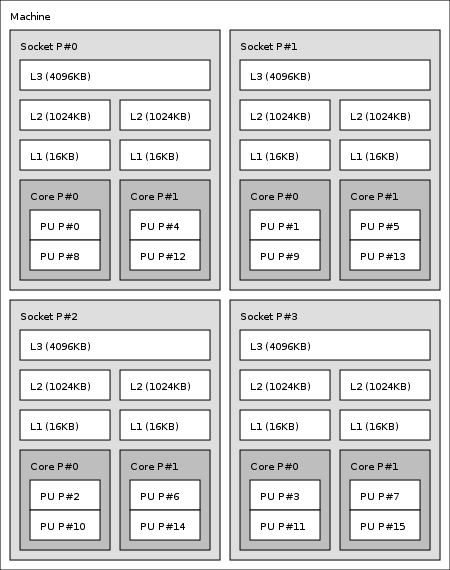
\includegraphics[width=9cm]{dudley.png}}
\end{DoxyImageNoCaption}


Here's the equivalent output in textual form:

\begin{DoxyVerb}
Machine (16GB)
  Socket L#0 + L3 L#0 (4096KB)
    L2 L#0 (1024KB) + L1 L#0 (16KB) + Core L#0
      PU L#0 (P#0)
      PU L#1 (P#8)
    L2 L#1 (1024KB) + L1 L#1 (16KB) + Core L#1
      PU L#2 (P#4)
      PU L#3 (P#12)
  Socket L#1 + L3 L#1 (4096KB)
    L2 L#2 (1024KB) + L1 L#2 (16KB) + Core L#2
      PU L#4 (P#1)
      PU L#5 (P#9)
    L2 L#3 (1024KB) + L1 L#3 (16KB) + Core L#3
      PU L#6 (P#5)
      PU L#7 (P#13)
  Socket L#2 + L3 L#2 (4096KB)
    L2 L#4 (1024KB) + L1 L#4 (16KB) + Core L#4
      PU L#8 (P#2)
      PU L#9 (P#10)
    L2 L#5 (1024KB) + L1 L#5 (16KB) + Core L#5
      PU L#10 (P#6)
      PU L#11 (P#14)
  Socket L#3 + L3 L#3 (4096KB)
    L2 L#6 (1024KB) + L1 L#6 (16KB) + Core L#6
      PU L#12 (P#3)
      PU L#13 (P#11)
    L2 L#7 (1024KB) + L1 L#7 (16KB) + Core L#7
      PU L#14 (P#7)
      PU L#15 (P#15)
\end{DoxyVerb}


Finally, here's the equivalent output in XML. Long lines were artificially broken for document clarity (in the real output, each XML tag is on a single line), and only socket \#0 is shown for brevity:

\begin{DoxyVerb}
<?xml version="1.0" encoding="UTF-8"?>
<!DOCTYPE topology SYSTEM "hwloc.dtd">
<topology>
  <object type="Machine" os_level="-1" os_index="0" cpuset="0x0000ffff" 
      complete_cpuset="0x0000ffff" online_cpuset="0x0000ffff" 
      allowed_cpuset="0x0000ffff" 
      dmi_board_vendor="Dell Computer Corporation" dmi_board_name="0RD318" 
      local_memory="16648183808">
    <page_type size="4096" count="4064498"/>
    <page_type size="2097152" count="0"/>
    <object type="Socket" os_level="-1" os_index="0" cpuset="0x00001111" 
        complete_cpuset="0x00001111" online_cpuset="0x00001111" 
        allowed_cpuset="0x00001111">
      <object type="Cache" os_level="-1" cpuset="0x00001111" 
          complete_cpuset="0x00001111" online_cpuset="0x00001111" 
          allowed_cpuset="0x00001111" cache_size="4194304" depth="3" 
          cache_linesize="64">
        <object type="Cache" os_level="-1" cpuset="0x00000101" 
            complete_cpuset="0x00000101" online_cpuset="0x00000101" 
            allowed_cpuset="0x00000101" cache_size="1048576" depth="2" 
            cache_linesize="64">
          <object type="Cache" os_level="-1" cpuset="0x00000101" 
              complete_cpuset="0x00000101" online_cpuset="0x00000101" 
              allowed_cpuset="0x00000101" cache_size="16384" depth="1" 
              cache_linesize="64">
            <object type="Core" os_level="-1" os_index="0" cpuset="0x00000101" 
                complete_cpuset="0x00000101" online_cpuset="0x00000101" 
                allowed_cpuset="0x00000101">
              <object type="PU" os_level="-1" os_index="0" cpuset="0x00000001" 
                  complete_cpuset="0x00000001" online_cpuset="0x00000001" 
                  allowed_cpuset="0x00000001"/>
              <object type="PU" os_level="-1" os_index="8" cpuset="0x00000100" 
                  complete_cpuset="0x00000100" online_cpuset="0x00000100" 
                  allowed_cpuset="0x00000100"/>
            </object>
          </object>
        </object>
        <object type="Cache" os_level="-1" cpuset="0x00001010" 
            complete_cpuset="0x00001010" online_cpuset="0x00001010" 
            allowed_cpuset="0x00001010" cache_size="1048576" depth="2" 
            cache_linesize="64">
          <object type="Cache" os_level="-1" cpuset="0x00001010" 
              complete_cpuset="0x00001010" online_cpuset="0x00001010" 
              allowed_cpuset="0x00001010" cache_size="16384" depth="1" 
              cache_linesize="64">
            <object type="Core" os_level="-1" os_index="1" cpuset="0x00001010" 
                complete_cpuset="0x00001010" online_cpuset="0x00001010" 
                allowed_cpuset="0x00001010">
              <object type="PU" os_level="-1" os_index="4" cpuset="0x00000010" 
                  complete_cpuset="0x00000010" online_cpuset="0x00000010" 
                  allowed_cpuset="0x00000010"/>
              <object type="PU" os_level="-1" os_index="12" cpuset="0x00001000" 
                  complete_cpuset="0x00001000" online_cpuset="0x00001000" 
                  allowed_cpuset="0x00001000"/>
            </object>
          </object>
        </object>
      </object>
    </object>
    <!-- ...other sockets listed here ... -->
  </object>
</topology>
\end{DoxyVerb}


On a 4-\/socket 2-\/core Opteron NUMA machine, the {\ttfamily lstopo-\/gui} tool may show the following graphical output:

 
\begin{DoxyImageNoCaption}
  \mbox{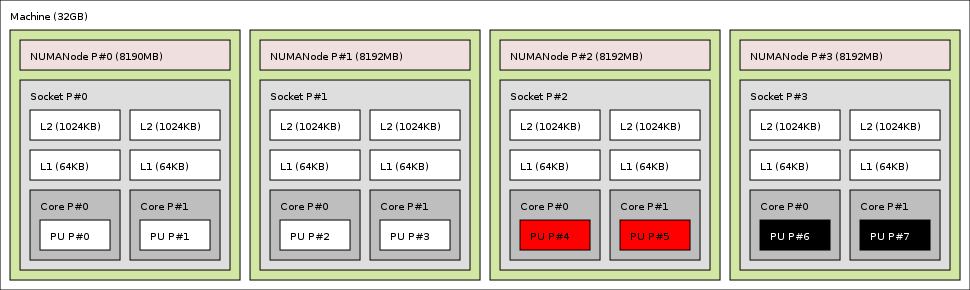
\includegraphics[width=\textwidth]{hagrid.png}}
\end{DoxyImageNoCaption}


Here's the equivalent output in textual form:

\begin{DoxyVerb}
Machine (32GB)
  NUMANode L#0 (P#0 8190MB) + Socket L#0
    L2 L#0 (1024KB) + L1 L#0 (64KB) + Core L#0 + PU L#0 (P#0)
    L2 L#1 (1024KB) + L1 L#1 (64KB) + Core L#1 + PU L#1 (P#1)
  NUMANode L#1 (P#1 8192MB) + Socket L#1
    L2 L#2 (1024KB) + L1 L#2 (64KB) + Core L#2 + PU L#2 (P#2)
    L2 L#3 (1024KB) + L1 L#3 (64KB) + Core L#3 + PU L#3 (P#3)
  NUMANode L#2 (P#2 8192MB) + Socket L#2
    L2 L#4 (1024KB) + L1 L#4 (64KB) + Core L#4 + PU L#4 (P#4)
    L2 L#5 (1024KB) + L1 L#5 (64KB) + Core L#5 + PU L#5 (P#5)
  NUMANode L#3 (P#3 8192MB) + Socket L#3
    L2 L#6 (1024KB) + L1 L#6 (64KB) + Core L#6 + PU L#6 (P#6)
    L2 L#7 (1024KB) + L1 L#7 (64KB) + Core L#7 + PU L#7 (P#7)
\end{DoxyVerb}


And here's the equivalent output in XML. Similar to above, line breaks were added and only PU \#0 is shown for brevity:

\begin{DoxyVerb}
<?xml version="1.0" encoding="UTF-8"?>
<!DOCTYPE topology SYSTEM "hwloc.dtd">
<topology>
  <object type="Machine" os_level="-1" os_index="0" cpuset="0x000000ff" 
      complete_cpuset="0x000000ff" online_cpuset="0x000000ff" 
      allowed_cpuset="0x000000ff" nodeset="0x000000ff" 
      complete_nodeset="0x000000ff" allowed_nodeset="0x000000ff" 
      dmi_board_vendor="TYAN Computer Corp" dmi_board_name="S4881 ">
    <page_type size="4096" count="0"/>
    <page_type size="2097152" count="0"/>
    <object type="NUMANode" os_level="-1" os_index="0" cpuset="0x00000003" 
        complete_cpuset="0x00000003" online_cpuset="0x00000003" 
        allowed_cpuset="0x00000003" nodeset="0x00000001" 
        complete_nodeset="0x00000001" allowed_nodeset="0x00000001" 
        local_memory="7514177536">
      <page_type size="4096" count="1834516"/>
      <page_type size="2097152" count="0"/>
      <object type="Socket" os_level="-1" os_index="0" cpuset="0x00000003" 
          complete_cpuset="0x00000003" online_cpuset="0x00000003" 
          allowed_cpuset="0x00000003" nodeset="0x00000001" 
          complete_nodeset="0x00000001" allowed_nodeset="0x00000001">
        <object type="Cache" os_level="-1" cpuset="0x00000001" 
            complete_cpuset="0x00000001" online_cpuset="0x00000001" 
            allowed_cpuset="0x00000001" nodeset="0x00000001" 
            complete_nodeset="0x00000001" allowed_nodeset="0x00000001" 
            cache_size="1048576" depth="2" cache_linesize="64">
          <object type="Cache" os_level="-1" cpuset="0x00000001" 
              complete_cpuset="0x00000001" online_cpuset="0x00000001" 
              allowed_cpuset="0x00000001" nodeset="0x00000001" 
              complete_nodeset="0x00000001" allowed_nodeset="0x00000001" 
              cache_size="65536" depth="1" cache_linesize="64">
            <object type="Core" os_level="-1" os_index="0" 
                cpuset="0x00000001" complete_cpuset="0x00000001" 
                online_cpuset="0x00000001" allowed_cpuset="0x00000001" 
                nodeset="0x00000001" complete_nodeset="0x00000001" 
                allowed_nodeset="0x00000001">
              <object type="PU" os_level="-1" os_index="0" cpuset="0x00000001" 
                  complete_cpuset="0x00000001" online_cpuset="0x00000001" 
                  allowed_cpuset="0x00000001" nodeset="0x00000001" 
                  complete_nodeset="0x00000001" allowed_nodeset="0x00000001"/>
            </object>
          </object>
        </object>
  <!-- ...more objects listed here ... -->
</topology>
\end{DoxyVerb}


On a 2-\/socket quad-\/core Xeon (pre-\/Nehalem, with 2 dual-\/core dies into each socket):

 
\begin{DoxyImageNoCaption}
  \mbox{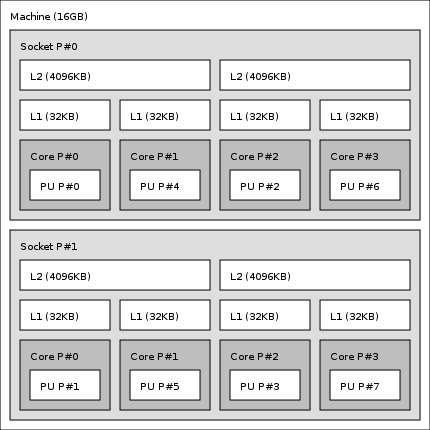
\includegraphics[width=7cm]{emmett.png}}
\end{DoxyImageNoCaption}


Here's the same output in textual form:

\begin{DoxyVerb}
Machine (16GB)
  Socket L#0
    L2 L#0 (4096KB)
      L1 L#0 (32KB) + Core L#0 + PU L#0 (P#0)
      L1 L#1 (32KB) + Core L#1 + PU L#1 (P#4)
    L2 L#1 (4096KB)
      L1 L#2 (32KB) + Core L#2 + PU L#2 (P#2)
      L1 L#3 (32KB) + Core L#3 + PU L#3 (P#6)
  Socket L#1
    L2 L#2 (4096KB)
      L1 L#4 (32KB) + Core L#4 + PU L#4 (P#1)
      L1 L#5 (32KB) + Core L#5 + PU L#5 (P#5)
    L2 L#3 (4096KB)
      L1 L#6 (32KB) + Core L#6 + PU L#6 (P#3)
      L1 L#7 (32KB) + Core L#7 + PU L#7 (P#7)
\end{DoxyVerb}


And the same output in XML (line breaks added, only PU \#0 shown):

\begin{DoxyVerb}
<?xml version="1.0" encoding="UTF-8"?>
<!DOCTYPE topology SYSTEM "hwloc.dtd">
<topology>
  <object type="Machine" os_level="-1" os_index="0" cpuset="0x000000ff" 
      complete_cpuset="0x000000ff" online_cpuset="0x000000ff" 
      allowed_cpuset="0x000000ff" dmi_board_vendor="Dell Inc." 
      dmi_board_name="0NR282" local_memory="16865292288">
    <page_type size="4096" count="4117503"/>
    <page_type size="2097152" count="0"/>
    <object type="Socket" os_level="-1" os_index="0" cpuset="0x00000055" 
        complete_cpuset="0x00000055" online_cpuset="0x00000055" 
        allowed_cpuset="0x00000055">
      <object type="Cache" os_level="-1" cpuset="0x00000011" 
          complete_cpuset="0x00000011" online_cpuset="0x00000011" 
          allowed_cpuset="0x00000011" cache_size="4194304" depth="2" 
          cache_linesize="64">
        <object type="Cache" os_level="-1" cpuset="0x00000001" 
            complete_cpuset="0x00000001" online_cpuset="0x00000001" 
            allowed_cpuset="0x00000001" cache_size="32768" depth="1" 
            cache_linesize="64">
          <object type="Core" os_level="-1" os_index="0" cpuset="0x00000001" 
              complete_cpuset="0x00000001" online_cpuset="0x00000001" 
              allowed_cpuset="0x00000001">
            <object type="PU" os_level="-1" os_index="0" cpuset="0x00000001" 
                complete_cpuset="0x00000001" online_cpuset="0x00000001" 
                allowed_cpuset="0x00000001"/>
          </object>
        </object>
        <object type="Cache" os_level="-1" cpuset="0x00000010" 
            complete_cpuset="0x00000010" online_cpuset="0x00000010" 
            allowed_cpuset="0x00000010" cache_size="32768" depth="1" 
            cache_linesize="64">
          <object type="Core" os_level="-1" os_index="1" cpuset="0x00000010" 
              complete_cpuset="0x00000010" online_cpuset="0x00000010" 
              allowed_cpuset="0x00000010">
            <object type="PU" os_level="-1" os_index="4" cpuset="0x00000010" 
                complete_cpuset="0x00000010" online_cpuset="0x00000010" 
                allowed_cpuset="0x00000010"/>
          </object>
        </object>
      </object>
  <!-- ...more objects listed here ... -->
</topology>
\end{DoxyVerb}


\hypertarget{index_interface}{}\section{Programming Interface}\label{index_interface}
The basic interface is available in \hyperlink{a00033_source}{hwloc.h}. It essentially offers low-\/level routines for advanced programmers that want to manually manipulate objects and follow links between them. Documentation for everything in \hyperlink{a00033_source}{hwloc.h} are provided later in this document. Developers should also look at \hyperlink{a00031_source}{hwloc/helper.h} (and also in this document, which provides good higher-\/level topology traversal examples).

To precisely define the vocabulary used by hwloc, a \hyperlink{a00001}{Terms and Definitions} section is available and should probably be read first.

Each hwloc object contains a cpuset describing the list of processing units that it contains. These bitmaps may be used for \hyperlink{a00049}{CPU binding} and \hyperlink{a00050}{Memory binding}. hwloc offers an extensive bitmap manipulation interface in \hyperlink{a00027_source}{hwloc/bitmap.h}.

Moreover, hwloc also comes with additional helpers for interoperability with several commonly used environments. See the \hyperlink{a00008}{Interoperability With Other Software} section for details.

The complete API documentation is available in a full set of HTML pages, man pages, and self-\/contained PDF files (formatted for both both US letter and A4 formats) in the source tarball in doc/doxygen-\/doc/.

{\bfseries NOTE:} If you are building the documentation from a Subversion checkout, you will need to have Doxygen and pdflatex installed -\/-\/ the documentation will be built during the normal \char`\"{}make\char`\"{} process. The documentation is installed during \char`\"{}make install\char`\"{} to \$prefix/share/doc/hwloc/ and your systems default man page tree (under \$prefix, of course).\hypertarget{index_portability}{}\subsection{Portability}\label{index_portability}
As shown in \hyperlink{index_cli_examples}{CLI Examples}, hwloc can obtain information on a wide variety of hardware topologies. However, some platforms and/or operating system versions will only report a subset of this information. For example, on an PPC64-\/based system with 32 cores (each with 2 hardware threads) running a default 2.6.18-\/based kernel from RHEL 5.4, hwloc is only able to glean information about NUMA nodes and processor units (PUs). No information about caches, sockets, or cores is available.

Similarly, Operating System have varying support for CPU and memory binding, e.g. while some Operating Systems provide interfaces for all kinds of CPU and memory bindings, some others provide only interfaces for a limited number of kinds of CPU and memory binding, and some do not provide any binding interface at all. Hwloc's binding functions would then simply return the ENOSYS error (Function not implemented), meaning that the underlying Operating System does not provide any interface for them. \hyperlink{a00049}{CPU binding} and \hyperlink{a00050}{Memory binding} provide more information on which hwloc binding functions should be preferred because interfaces for them are usually available on the supported Operating Systems.

Here's the graphical output from lstopo-\/gui on this platform when Simultaneous Multi-\/Threading (SMT) is enabled:

 
\begin{DoxyImageNoCaption}
  \mbox{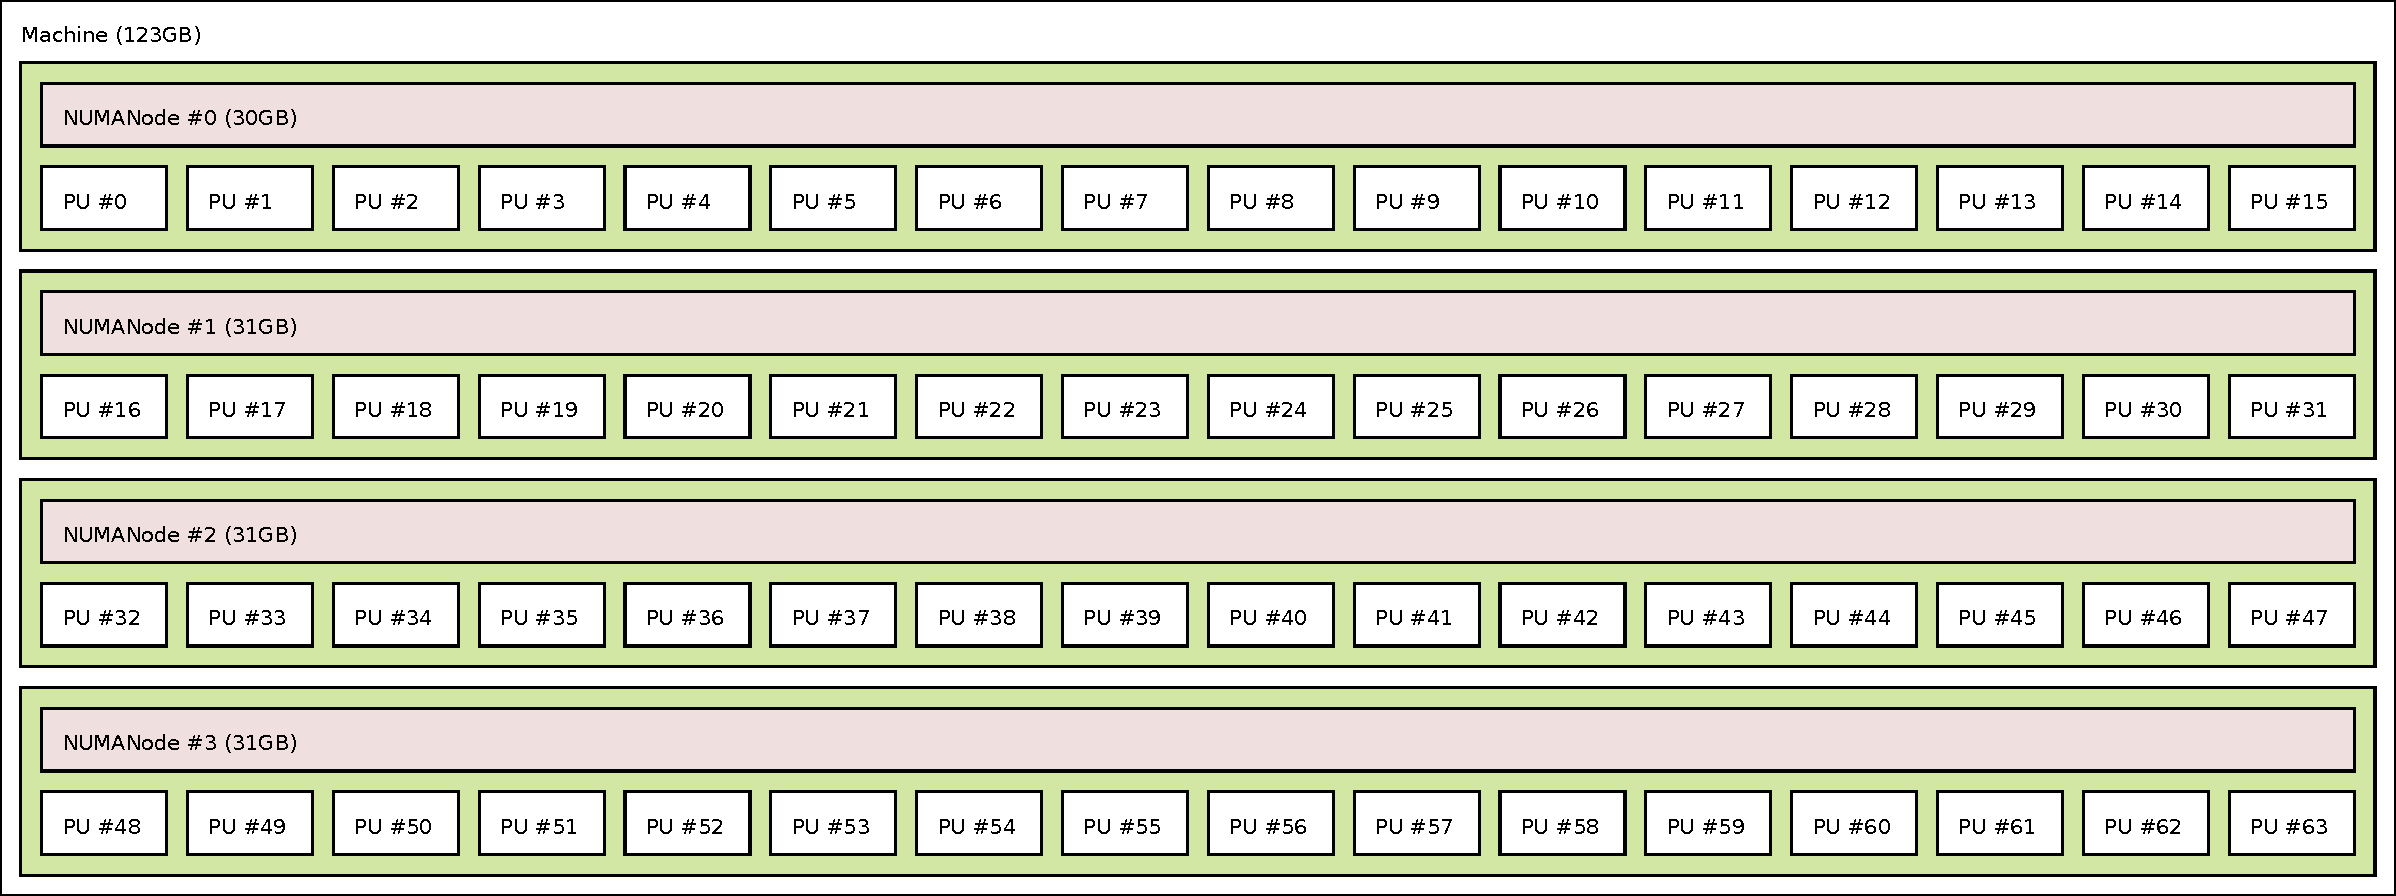
\includegraphics[width=\textwidth]{ppc64-with-smt}}
\end{DoxyImageNoCaption}


And here's the graphical output from lstopo-\/gui on this platform when SMT is disabled:

 
\begin{DoxyImageNoCaption}
  \mbox{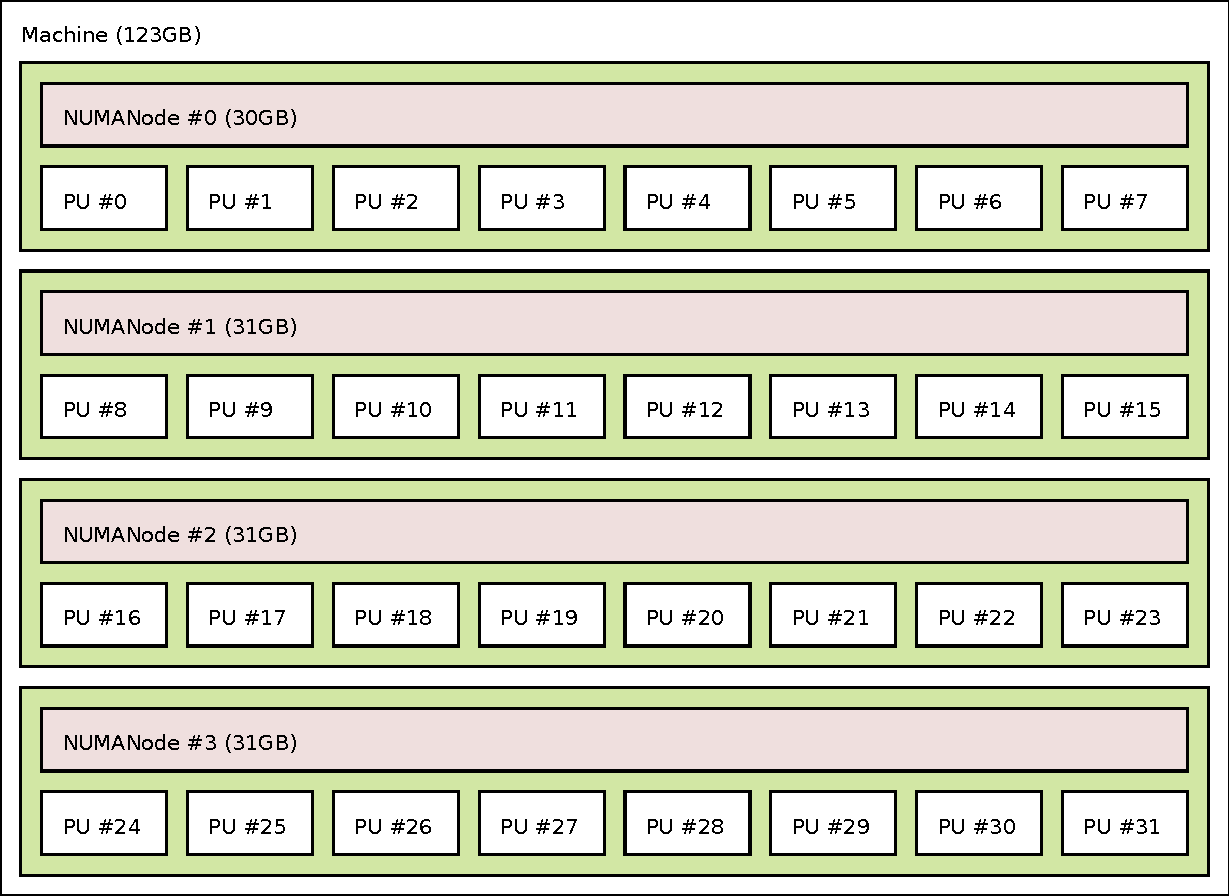
\includegraphics[width=\textwidth]{ppc64-without-smt}}
\end{DoxyImageNoCaption}


Notice that hwloc only sees half the PUs when SMT is disabled. PU \#15, for example, seems to change location from NUMA node \#0 to \#1. In reality, no PUs \char`\"{}moved\char`\"{} -\/-\/ they were simply re-\/numbered when hwloc only saw half as many. Hence, PU \#15 in the SMT-\/disabled picture probably corresponds to PU \#30 in the SMT-\/enabled picture.

This same \char`\"{}PUs have disappeared\char`\"{} effect can be seen on other platforms -\/-\/ even platforms / OSs that provide much more information than the above PPC64 system. This is an unfortunate side-\/effect of how operating systems report information to hwloc.

Note that upgrading the Linux kernel on the same PPC64 system mentioned above to 2.6.34, hwloc is able to discover all the topology information. The following picture shows the entire topology layout when SMT is enabled:

 
\begin{DoxyImageNoCaption}
  \mbox{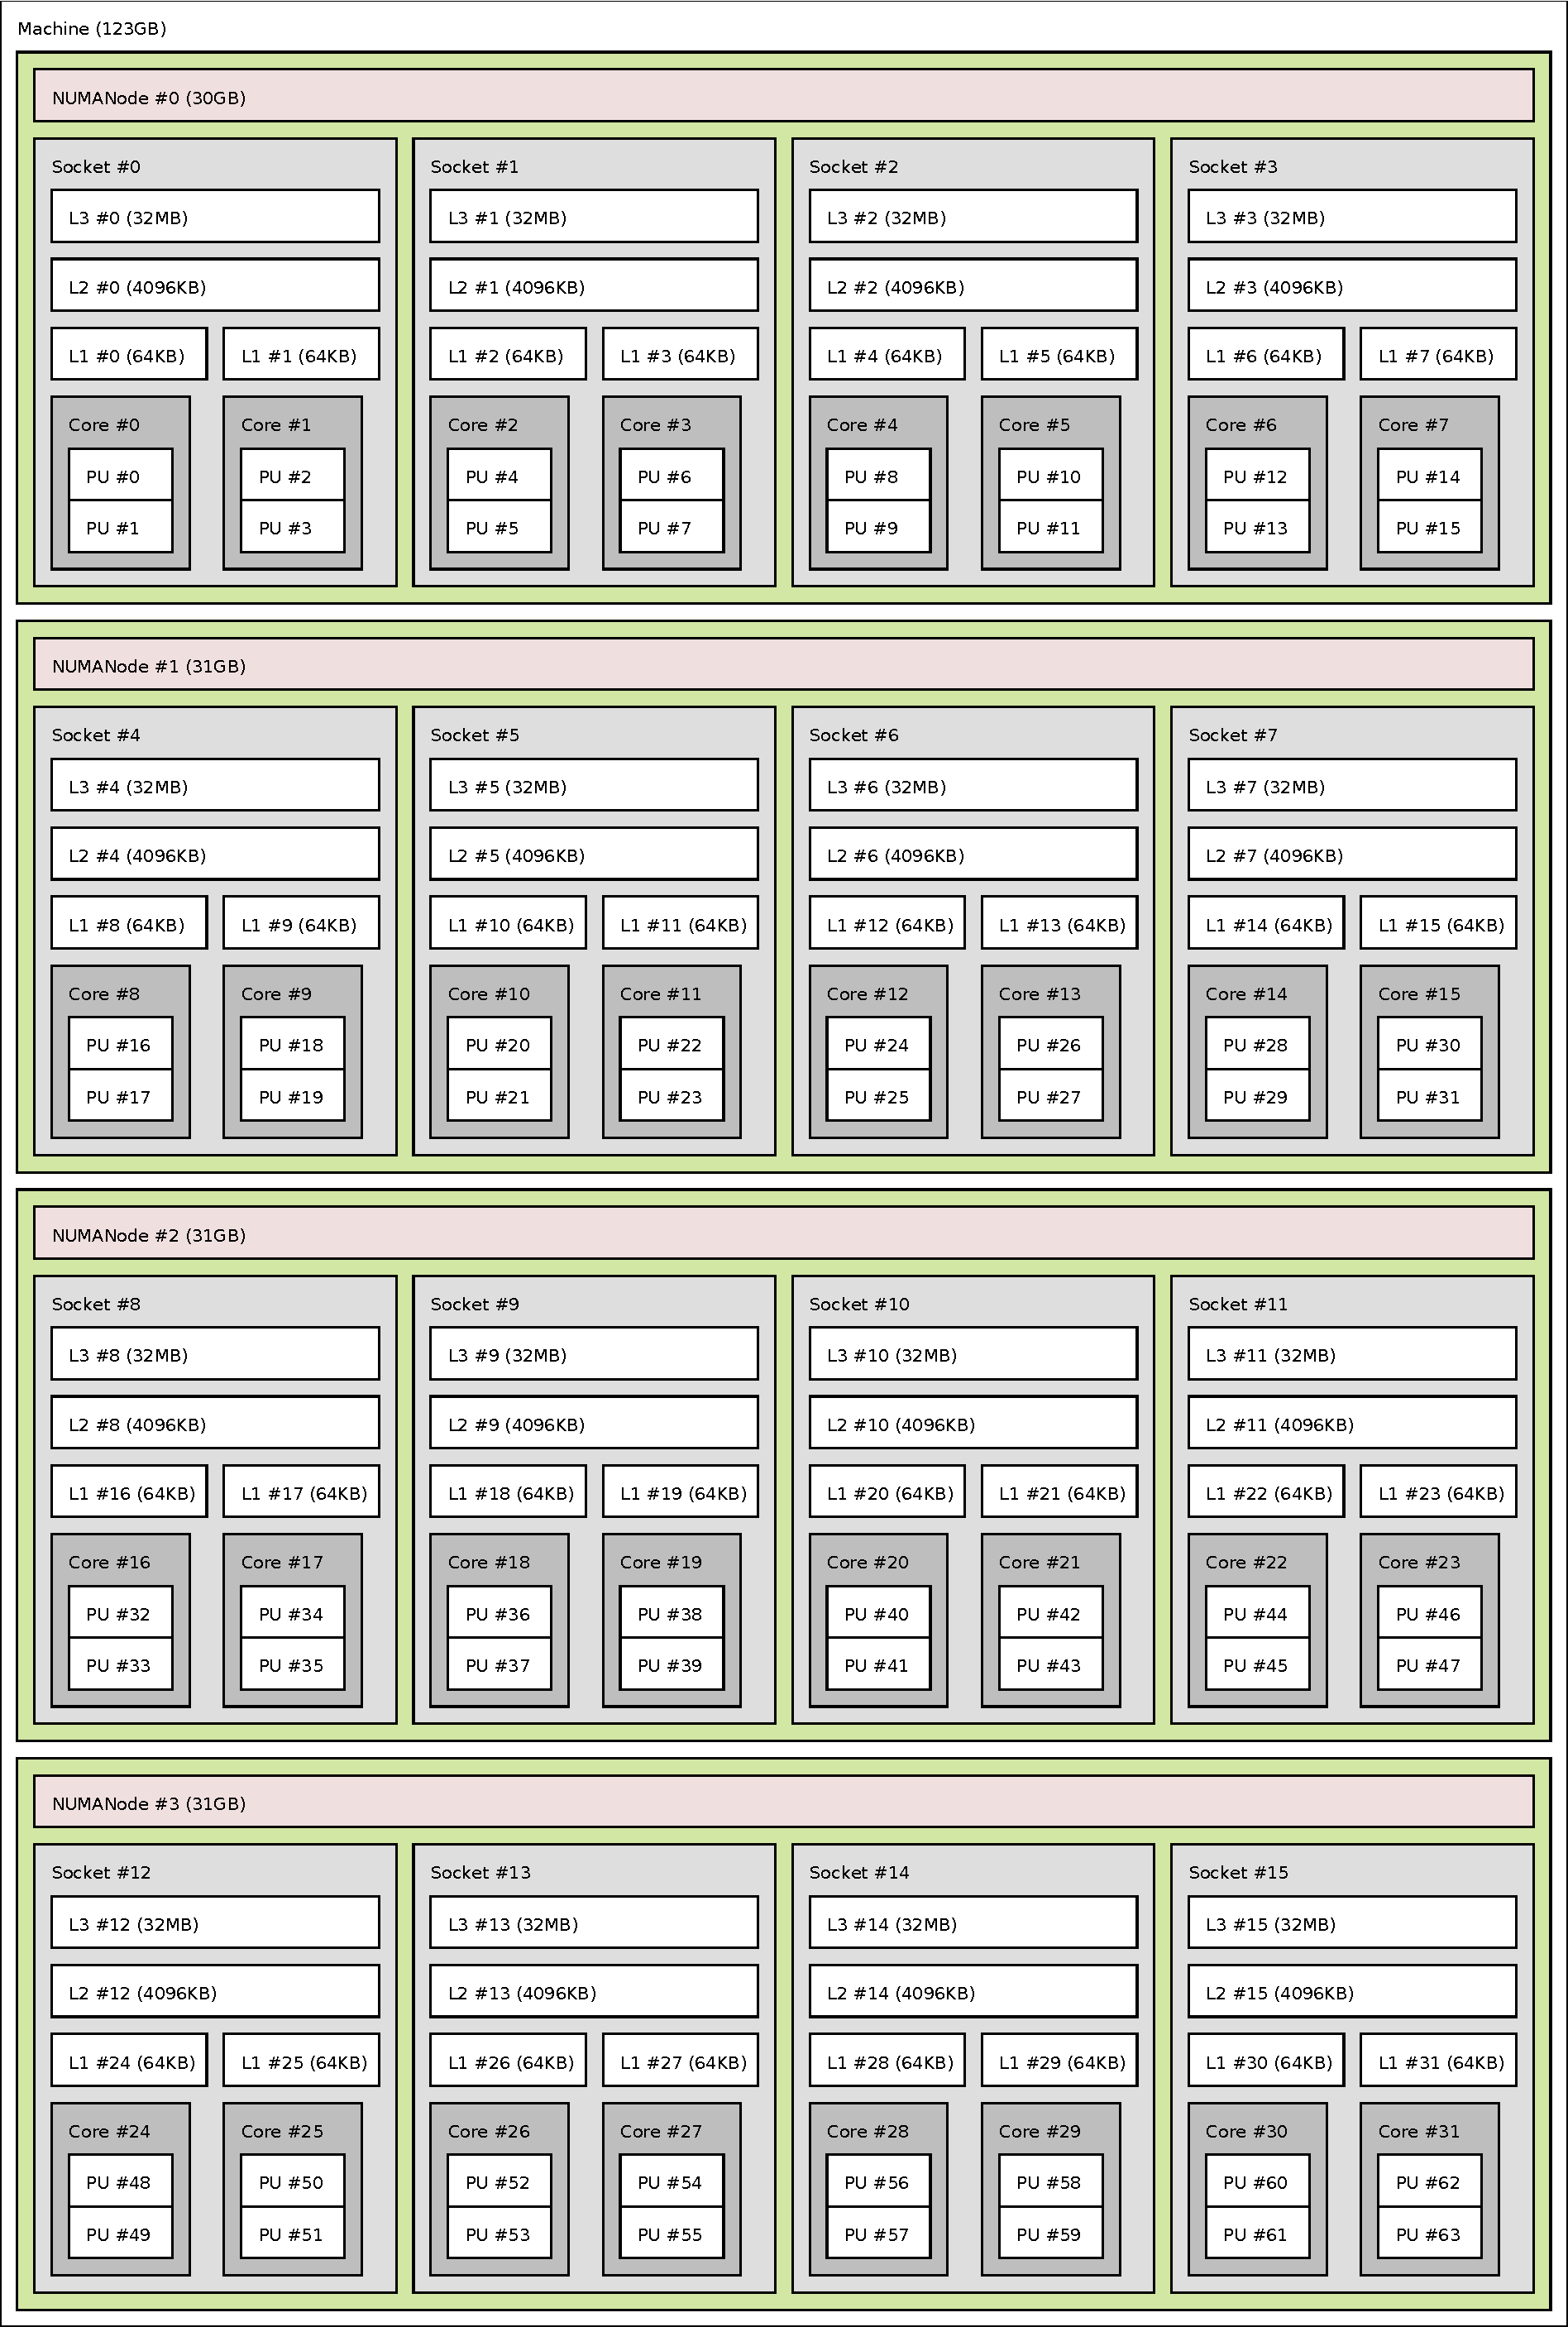
\includegraphics[width=\textwidth]{ppc64-full-with-smt}}
\end{DoxyImageNoCaption}


Developers using the hwloc API or XML output for portable applications should therefore be extremely careful to not make any assumptions about the structure of data that is returned. For example, per the above reported PPC topology, it is not safe to assume that PUs will always be descendants of cores.

Additionally, future hardware may insert new topology elements that are not available in this version of hwloc. Long-\/lived applications that are meant to span multiple different hardware platforms should also be careful about making structure assumptions. For example, there may someday be an element \char`\"{}lower\char`\"{} than a PU, or perhaps a new element may exist between a core and a PU.\hypertarget{index_interface_example}{}\subsection{API Example}\label{index_interface_example}
The following small C example (named ``hwloc-\/hello.c'') prints the topology of the machine and bring the process to the first logical processor of the second core of the machine.


\begin{DoxyCodeInclude}
\textcolor{comment}{/* Example hwloc API program.}
\textcolor{comment}{ *}
\textcolor{comment}{ * Copyright © 2009-2010 inria.  All rights reserved.}
\textcolor{comment}{ * Copyright © 2009-2011 Université Bordeaux 1}
\textcolor{comment}{ * Copyright © 2009-2010 Cisco Systems, Inc.  All rights reserved.}
\textcolor{comment}{ * See COPYING in top-level directory.}
\textcolor{comment}{ *}
\textcolor{comment}{ * hwloc-hello.c}
\textcolor{comment}{ */}

\textcolor{preprocessor}{#include <hwloc.h>}
\textcolor{preprocessor}{#include <errno.h>}
\textcolor{preprocessor}{#include <stdio.h>}
\textcolor{preprocessor}{#include <string.h>}

\textcolor{keyword}{static} \textcolor{keywordtype}{void} print\_children(\hyperlink{a00039_ga9d1e76ee15a7dee158b786c30b6a6e38}{hwloc_topology_t} topology, \hyperlink{a00016}{hwloc_obj_t} obj, 
                           \textcolor{keywordtype}{int} depth)
\{
    \textcolor{keywordtype}{char} \textcolor{keywordtype}{string}[128];
    \textcolor{keywordtype}{unsigned} i;

    \hyperlink{a00048_ga5c6a61a83f4790b421e2f62e9088446f}{hwloc_obj_snprintf}(\textcolor{keywordtype}{string}, \textcolor{keyword}{sizeof}(\textcolor{keywordtype}{string}), topology, obj, \textcolor{stringliteral}{"#"}, 0);
    printf(\textcolor{stringliteral}{"%*s%s\(\backslash\)n"}, 2*depth, \textcolor{stringliteral}{""}, \textcolor{keywordtype}{string});
    \textcolor{keywordflow}{for} (i = 0; i < obj->\hyperlink{a00016_aac3f6da35c9b57599909a44ce2b716c1}{arity}; i++) \{
        print\_children(topology, obj->\hyperlink{a00016_a04d05403da37bfe17cd63b7c7dd07b1f}{children}[i], depth + 1);
    \}
\}

\textcolor{keywordtype}{int} main(\textcolor{keywordtype}{void})
\{
    \textcolor{keywordtype}{int} depth;
    \textcolor{keywordtype}{unsigned} i, n;
    \textcolor{keywordtype}{unsigned} \textcolor{keywordtype}{long} size;
    \textcolor{keywordtype}{int} levels;
    \textcolor{keywordtype}{char} \textcolor{keywordtype}{string}[128];
    \textcolor{keywordtype}{int} topodepth;
    \hyperlink{a00039_ga9d1e76ee15a7dee158b786c30b6a6e38}{hwloc_topology_t} topology;
    \hyperlink{a00040_ga4bbf39b68b6f568fb92739e7c0ea7801}{hwloc_cpuset_t} cpuset;
    \hyperlink{a00016}{hwloc_obj_t} obj;

    \textcolor{comment}{/* Allocate and initialize topology object. */}
    \hyperlink{a00043_ga5c2d6f476af87005c7bd0811d4548b9f}{hwloc_topology_init}(&topology);

    \textcolor{comment}{/* ... Optionally, put detection configuration here to ignore}
\textcolor{comment}{       some objects types, define a synthetic topology, etc....  }
\textcolor{comment}{}
\textcolor{comment}{       The default is to detect all the objects of the machine that}
\textcolor{comment}{       the caller is allowed to access.  See Configure Topology}
\textcolor{comment}{       Detection. */}

    \textcolor{comment}{/* Perform the topology detection. */}
    \hyperlink{a00043_ga91e2e6427b95fb7339c99dbbef996e71}{hwloc_topology_load}(topology);

    \textcolor{comment}{/* Optionally, get some additional topology information}
\textcolor{comment}{       in case we need the topology depth later. */}
    topodepth = \hyperlink{a00046_ga8c30b0cec55074eb3ed34e4f2a1a9937}{hwloc_topology_get_depth}(topology);

    \textcolor{comment}{/*****************************************************************}
\textcolor{comment}{     * First example:}
\textcolor{comment}{     * Walk the topology with an array style, from level 0 (always}
\textcolor{comment}{     * the system level) to the lowest level (always the proc level).}
\textcolor{comment}{     *****************************************************************/}
    \textcolor{keywordflow}{for} (depth = 0; depth < topodepth; depth++) \{
        printf(\textcolor{stringliteral}{"*** Objects at level %d\(\backslash\)n"}, depth);
        \textcolor{keywordflow}{for} (i = 0; i < \hyperlink{a00046_ga20cfe2456f4cfdd789c9aca6d2fdd69f}{hwloc_get_nbobjs_by_depth}(topology, depth); 
             i++) \{
            \hyperlink{a00048_ga5c6a61a83f4790b421e2f62e9088446f}{hwloc_obj_snprintf}(\textcolor{keywordtype}{string}, \textcolor{keyword}{sizeof}(\textcolor{keywordtype}{string}), topology,
                       \hyperlink{a00047_gaedd78240b0c1108355586a268ec5a697}{hwloc_get_obj_by_depth}(topology, depth, i),
                       \textcolor{stringliteral}{"#"}, 0);
            printf(\textcolor{stringliteral}{"Index %u: %s\(\backslash\)n"}, i, \textcolor{keywordtype}{string});
        \}
    \}

    \textcolor{comment}{/*****************************************************************}
\textcolor{comment}{     * Second example:}
\textcolor{comment}{     * Walk the topology with a tree style.}
\textcolor{comment}{     *****************************************************************/}
    printf(\textcolor{stringliteral}{"*** Printing overall tree\(\backslash\)n"});
    print\_children(topology, \hyperlink{a00053_gadbf58f6e187efbdb3cd9a8e30311b7d7}{hwloc_get_root_obj}(topology), 0);

    \textcolor{comment}{/*****************************************************************}
\textcolor{comment}{     * Third example:}
\textcolor{comment}{     * Print the number of sockets.}
\textcolor{comment}{     *****************************************************************/}
    depth = \hyperlink{a00046_gaea7c64dd59467f5201ba87712710b14d}{hwloc_get_type_depth}(topology, \hyperlink{a00041_ggacd37bb612667dc437d66bfb175a8dc55a1ac6e07775ae4324b3fe9dbd72c785ec}{HWLOC_OBJ_SOCKET});
    \textcolor{keywordflow}{if} (depth == \hyperlink{a00046_ggaf4e663cf42bbe20756b849c6293ef575a0565ab92ab72cb0cec91e23003294aad}{HWLOC_TYPE_DEPTH_UNKNOWN}) \{
        printf(\textcolor{stringliteral}{"*** The number of sockets is unknown\(\backslash\)n"});
    \} \textcolor{keywordflow}{else} \{
        printf(\textcolor{stringliteral}{"*** %u socket(s)\(\backslash\)n"}, 
               \hyperlink{a00046_ga20cfe2456f4cfdd789c9aca6d2fdd69f}{hwloc_get_nbobjs_by_depth}(topology, depth));
    \}

    \textcolor{comment}{/*****************************************************************}
\textcolor{comment}{     * Fourth example:}
\textcolor{comment}{     * Compute the amount of cache that the first logical processor}
\textcolor{comment}{     * has above it.}
\textcolor{comment}{     *****************************************************************/}
    levels = 0;
    size = 0;
    \textcolor{keywordflow}{for} (obj = \hyperlink{a00047_ga9be4a03488cdd0fb431e4aa1cbdea895}{hwloc_get_obj_by_type}(topology, \hyperlink{a00041_ggacd37bb612667dc437d66bfb175a8dc55abca6887e80cb291353b0a0c1da83f661}{HWLOC_OBJ_PU}, 0);
         obj;
         obj = obj->\hyperlink{a00016_adc494f6aed939992be1c55cca5822900}{parent})
      \textcolor{keywordflow}{if} (obj->\hyperlink{a00016_acc4f0803f244867e68fe0036800be5de}{type} == \hyperlink{a00041_ggacd37bb612667dc437d66bfb175a8dc55a56ee0b7eca88f363b75b34fdde8c9ddc}{HWLOC_OBJ_CACHE}) \{
        levels++;
        size += obj->\hyperlink{a00016_accd40e29f71f19e88db62ea3df02adc8}{attr}->\hyperlink{a00017_ab5a8ae3bf490e6b1071fea53f7382836}{cache}.\hyperlink{a00013_abe5e788943ed04302976740c829674c0}{size};
      \}
    printf(\textcolor{stringliteral}{"*** Logical processor 0 has %d caches totaling %luKB\(\backslash\)n"}, 
           levels, size / 1024);

    \textcolor{comment}{/*****************************************************************}
\textcolor{comment}{     * Fifth example:}
\textcolor{comment}{     * Bind to only one thread of the last core of the machine.}
\textcolor{comment}{     *}
\textcolor{comment}{     * First find out where cores are, or else smaller sets of CPUs if}
\textcolor{comment}{     * the OS doesn't have the notion of a "core".}
\textcolor{comment}{     *****************************************************************/}
    depth = \hyperlink{a00052_ga081be77905201e9f42318e9974456b45}{hwloc_get_type_or_below_depth}(topology, \hyperlink{a00041_ggacd37bb612667dc437d66bfb175a8dc55ac793958f330bca371aa1535de8aff45f}{HWLOC_OBJ_CORE});

    \textcolor{comment}{/* Get last core. */}
    obj = \hyperlink{a00047_gaedd78240b0c1108355586a268ec5a697}{hwloc_get_obj_by_depth}(topology, depth,
                   \hyperlink{a00046_ga20cfe2456f4cfdd789c9aca6d2fdd69f}{hwloc_get_nbobjs_by_depth}(topology, depth) - 1);
    \textcolor{keywordflow}{if} (obj) \{
        \textcolor{comment}{/* Get a copy of its cpuset that we may modify. */}
        cpuset = \hyperlink{a00065_gaaa4ed76211cd3694dfbea2109fc440be}{hwloc_bitmap_dup}(obj->\hyperlink{a00016_a67925e0f2c47f50408fbdb9bddd0790f}{cpuset});

        \textcolor{comment}{/* Get only one logical processor (in case the core is}
\textcolor{comment}{           SMT/hyperthreaded). */}
        \hyperlink{a00065_ga4630aa1b7e08eac5b41be126194e84a1}{hwloc_bitmap_singlify}(cpuset);

        \textcolor{comment}{/* And try to bind ourself there. */}
        \textcolor{keywordflow}{if} (\hyperlink{a00049_gaf4cc194d5c0d38004a21b9f03522a7e3}{hwloc_set_cpubind}(topology, cpuset, 0)) \{
            \textcolor{keywordtype}{char} *str;
            \textcolor{keywordtype}{int} error = errno;
            \hyperlink{a00065_gad3cf87ceb58aa91656756bbb58057320}{hwloc_bitmap_asprintf}(&str, obj->\hyperlink{a00016_a67925e0f2c47f50408fbdb9bddd0790f}{cpuset});
            printf(\textcolor{stringliteral}{"Couldn't bind to cpuset %s: %s\(\backslash\)n"}, str, strerror(error));
            free(str);
        \}

        \textcolor{comment}{/* Free our cpuset copy */}
        \hyperlink{a00065_ga8e7035fe555ef96921bfb98e08519bc7}{hwloc_bitmap_free}(cpuset);
    \}

    \textcolor{comment}{/*****************************************************************}
\textcolor{comment}{     * Sixth example:}
\textcolor{comment}{     * Allocate some memory on the last NUMA node, bind some existing}
\textcolor{comment}{     * memory to the last NUMA node.}
\textcolor{comment}{     *****************************************************************/}
    \textcolor{comment}{/* Get last node. */}
    n = \hyperlink{a00046_gaba821f84ef64282d14577066e6d6547e}{hwloc_get_nbobjs_by_type}(topology, \hyperlink{a00041_ggacd37bb612667dc437d66bfb175a8dc55aaf0964881117bdedf1a5e9332cd120dd}{HWLOC_OBJ_NODE});
    \textcolor{keywordflow}{if} (n) \{
        \textcolor{keywordtype}{void} *m;
        size = 1024*1024;

        obj = \hyperlink{a00047_ga9be4a03488cdd0fb431e4aa1cbdea895}{hwloc_get_obj_by_type}(topology, \hyperlink{a00041_ggacd37bb612667dc437d66bfb175a8dc55aaf0964881117bdedf1a5e9332cd120dd}{HWLOC_OBJ_NODE}, n - 1);
        m = \hyperlink{a00050_gaeaa00714a9c4319bda0a74ca6f8720e8}{hwloc_alloc_membind_nodeset}(topology, size, obj->\hyperlink{a00016_a08f0d0e16c619a6e653526cbee4ffea3}{nodeset},
                \hyperlink{a00050_ggac9764f79505775d06407b40f5e4661e8a18675bb80ebc1bce5b652e9de8f3998c}{HWLOC_MEMBIND_DEFAULT}, 0);
        \hyperlink{a00050_ga986d9b4cc76da592c4b937c6cb7d9d56}{hwloc_free}(topology, m, size);

        m = malloc(size);
        \hyperlink{a00050_gade5e2c28ea8475a479bf2b1df36c6ccd}{hwloc_set_area_membind_nodeset}(topology, m, size, obj->\hyperlink{a00016_a08f0d0e16c619a6e653526cbee4ffea3}{nodeset},
                \hyperlink{a00050_ggac9764f79505775d06407b40f5e4661e8a18675bb80ebc1bce5b652e9de8f3998c}{HWLOC_MEMBIND_DEFAULT}, 0);
        free(m);
    \}

    \textcolor{comment}{/* Destroy topology object. */}
    \hyperlink{a00043_ga6040925d3ee4bbb2647f2a321aca5f4b}{hwloc_topology_destroy}(topology);

    \textcolor{keywordflow}{return} 0;
\}
\end{DoxyCodeInclude}


hwloc provides a {\ttfamily pkg-\/config} executable to obtain relevant compiler and linker flags. For example, it can be used thusly to compile applications that utilize the hwloc library (assuming GNU Make):

\begin{DoxyVerb}
CFLAGS += $(pkg-config --cflags hwloc)
LDLIBS += $(pkg-config --libs hwloc)
cc hwloc-hello.c $(CFLAGS) -o hwloc-hello $(LDLIBS)
\end{DoxyVerb}


On a machine with 4GB of RAM and 2 processor sockets -\/-\/ each socket of which has two processing cores -\/-\/ the output from running {\ttfamily hwloc-\/hello} could be something like the following:

\begin{DoxyVerb}
shell$ ./hwloc-hello
*** Objects at level 0
Index 0: Machine(3938MB)
*** Objects at level 1
Index 0: Socket#0
Index 1: Socket#1
*** Objects at level 2
Index 0: Core#0
Index 1: Core#1
Index 2: Core#3
Index 3: Core#2
*** Objects at level 3
Index 0: PU#0
Index 1: PU#1
Index 2: PU#2
Index 3: PU#3
*** Printing overall tree
Machine(3938MB)
  Socket#0
    Core#0
      PU#0
    Core#1
      PU#1
  Socket#1
    Core#3
      PU#2
    Core#2
      PU#3
*** 2 socket(s)
shell$ 
\end{DoxyVerb}


 \hypertarget{index_bugs}{}\section{Questions and Bugs}\label{index_bugs}
Questions should be sent to the devel mailing list (\href{http://www.open-mpi.org/community/lists/hwloc.php}{\tt http://www.open-\/mpi.org/community/lists/hwloc.php}). Bug reports should be reported in the tracker (\href{https://svn.open-mpi.org/trac/hwloc/}{\tt https://svn.open-\/mpi.org/trac/hwloc/}).

If hwloc discovers an incorrect topology for your machine, the very first thing you should check is to ensure that you have the most recent updates installed for your operating system. Indeed, most of hwloc topology discovery relies on hardware information retrieved through the operation system (e.g., via the /sys virtual filesystem of the Linux kernel). If upgrading your OS or Linux kernel does not solve your problem, you may also want to ensure that you are running the most recent version of the BIOS for your machine.

If those things fail, contact us on the mailing list for additional help. Please attach the output of lstopo after having given the -\/-\/enable-\/debug option to ./configure and rebuilt completely, to get debugging output. Also attach the {\ttfamily /proc} + {\ttfamily /sys} tarball generated by the installed script {\ttfamily hwloc-\/gather-\/topology.sh} when submitting problems about Linux, or send the output of {\ttfamily kstat cpu\_\-info} in the Solaris case, or the output of {\ttfamily sysctl hw} in the Darwin or BSD cases.

 \hypertarget{index_history}{}\section{History / Credits}\label{index_history}
hwloc is the evolution and merger of the libtopology (\href{http://runtime.bordeaux.inria.fr/libtopology/}{\tt http://runtime.bordeaux.inria.fr/libtopology/}) project and the Portable Linux Processor Affinity (PLPA) (\href{http://www.open-mpi.org/projects/plpa/}{\tt http://www.open-\/mpi.org/projects/plpa/}) project. Because of functional and ideological overlap, these two code bases and ideas were merged and released under the name \char`\"{}hwloc\char`\"{} as an Open MPI sub-\/project.

libtopology was initially developed by the inria Runtime Team-\/Project (\href{http://runtime.bordeaux.inria.fr/}{\tt http://runtime.bordeaux.inria.fr/}) (headed by Raymond Namyst (\href{http://dept-info.labri.fr/~namyst/}{\tt http://dept-\/info.labri.fr/$\sim$namyst/}). PLPA was initially developed by the Open MPI development team as a sub-\/project. Both are now deprecated in favor of hwloc, which is distributed as an Open MPI sub-\/project.

 \hypertarget{index_further_read}{}\section{Further Reading}\label{index_further_read}
The documentation chapters include


\begin{DoxyItemize}
\item \hyperlink{a00001}{Terms and Definitions} 
\item \hyperlink{a00002}{Command-\/Line Tools} 
\item \hyperlink{a00003}{Environment Variables} 
\item \hyperlink{a00004}{CPU and Memory Binding Overview} 
\item \hyperlink{a00005}{I/O Devices} 
\item \hyperlink{a00006}{Multi-\/node Topologies} 
\item \hyperlink{a00007}{Importing and exporting topologies from/to XML files} 
\item \hyperlink{a00008}{Interoperability With Other Software} 
\item \hyperlink{a00009}{Thread Safety} 
\item \hyperlink{a00010}{Embedding hwloc in Other Software} 
\item \hyperlink{a00011}{Frequently Asked Questions} 
\end{DoxyItemize}

Make sure to have had a look at those too!

 
\chapter{Terms and Definitions}
\label{termsanddefs}
\hypertarget{termsanddefs}{}

\begin{DoxyDescription}
\item[Object ]Interesting kind of part of the system, such as a Core, a Cache, a Memory node, etc. The different types detected by hwloc are detailed in the \hyperlink{a00041_gacd37bb612667dc437d66bfb175a8dc55}{hwloc\_\-obj\_\-type\_\-t} enumeration.

They are topologically sorted by CPU set into a tree. 


\item[CPU set ]The set of logical processors (or processing units) logically included in an object (if it makes sense). They are always expressed using physical logical processor numbers (as announced by the OS). They are implemented as the \hyperlink{a00065_gaa3c2bf4c776d603dcebbb61b0c923d84}{hwloc\_\-bitmap\_\-t} opaque structure. hwloc CPU sets are just masks, they do {\itshape not\/} have any relation with an operating system actual binding notion like Linux' cpusets.


\item[Node set ]The set of NUMA memory nodes logically included in an object (if it makes sense). They are always expressed using physical node numbers (as announced by the OS). They are implemented with the \hyperlink{a00065_gaa3c2bf4c776d603dcebbb61b0c923d84}{hwloc\_\-bitmap\_\-t} opaque structure. as bitmaps.


\item[Bitmap ]A possibly-\/infinite set of bits used for describing sets of objects such as CPUs (CPU sets) or memory nodes (Node sets). They are implemented with the \hyperlink{a00065_gaa3c2bf4c776d603dcebbb61b0c923d84}{hwloc\_\-bitmap\_\-t} opaque structure. 


\item[Parent object ]The object logically containing the current object, for example because its CPU set includes the CPU set of the current object.


\item[Ancestor object ]The parent object, or its own parent object, and so on.


\item[Children object(s) ]The object (or objects) contained in the current object because their CPU set is included in the CPU set of the current object.


\item[Arity ]The number of children of an object.


\item[Sibling objects ]Objects which have the same parent. They usually have the same type (and hence are cousins, as well), but they may not if the topology is asymmetric.


\item[Sibling rank ]Index to uniquely identify objects which have the same parent, and is always in the range \mbox{[}0, parent\_\-arity).


\item[Cousin objects ]Objects of the same type (and depth) as the current object, even if they do not have the same parent.


\item[Level ]Set of objects of the same type and depth. All these objects are cousins.


\item[Depth ]Nesting level in the object tree, starting from the root object. If the topology is symmetric, the depth of a child is equal to the parent depth plus one, and an object depth is also equal to the number of parent/child links between the root object and the given object. If the topology is asymmetric, the difference between some parent and child depths may be larger than one when some intermediate levels (for instance caches) are missing in only some parts of the machine. 


\item[OS or physical index ]The index that the operating system (OS) uses to identify the object. This may be completely arbitrary, non-\/unique, non-\/contiguous, not representative of logical proximity, and may depend on the BIOS configuration. That is why hwloc almost never uses them, only in the default lstopo output ({\ttfamily P::x}) and cpuset masks.


\item[Logical index ]Index to uniquely identify objects of the same type and depth, automatically computed by hwloc according to the topology. It expresses logical proximity in a generic way, i.e. objects which have adjacent logical indexes are adjacent in the topology. That is why hwloc almost always uses it in its API, since it expresses logical proximity. They can be shown (as {\ttfamily L::x}) by {\ttfamily lstopo} thanks to the {\ttfamily -\/l} option. This index is always linear and in the range \mbox{[}0, num\_\-objs\_\-same\_\-type\_\-same\_\-level-\/1\mbox{]}. Think of it as ``cousin rank.'' The ordering is based on topology first, and then on OS CPU numbers, so it is stable across everything except firmware CPU renumbering. \char`\"{}Logical index\char`\"{} should not be confused with \char`\"{}Logical processor\char`\"{}. A \char`\"{}Logical
  processor\char`\"{} (which in hwloc we rather call \char`\"{}processing unit\char`\"{} to avoid the confusion) has both a physical index (as chosen arbitrarily by BIOS/OS) and a logical index (as computed according to logical proximity by hwloc). 


\item[Logical processor ]
\item[Processing unit ]The smallest processing element that can be represented by a hwloc object. It may be a single-\/core processor, a core of a multicore processor, or a single thread in SMT processor. \char`\"{}Logical processor\char`\"{} should not be confused with \char`\"{}Logical index of a
  processor\char`\"{}. \char`\"{}Logical processor\char`\"{} is only one of the names which can be found in various documentations to designate a processing unit. 


\end{DoxyDescription}

The following diagram can help to understand the vocabulary of the relationships by showing the example of a machine with two dual core sockets (with no hardware threads); thus, a topology with 4 levels. Each box with rounded corner corresponds to one hwloc\_\-obj\_\-t, containing the values of the different integer fields (depth, logical\_\-index, etc.), and arrows show to which other hwloc\_\-obj\_\-t pointers point to (first\_\-child, parent, etc.). The L2 cache of the last core is intentionally missing to show how asymmetric topologies are handled.

 
\begin{DoxyImageNoCaption}
  \mbox{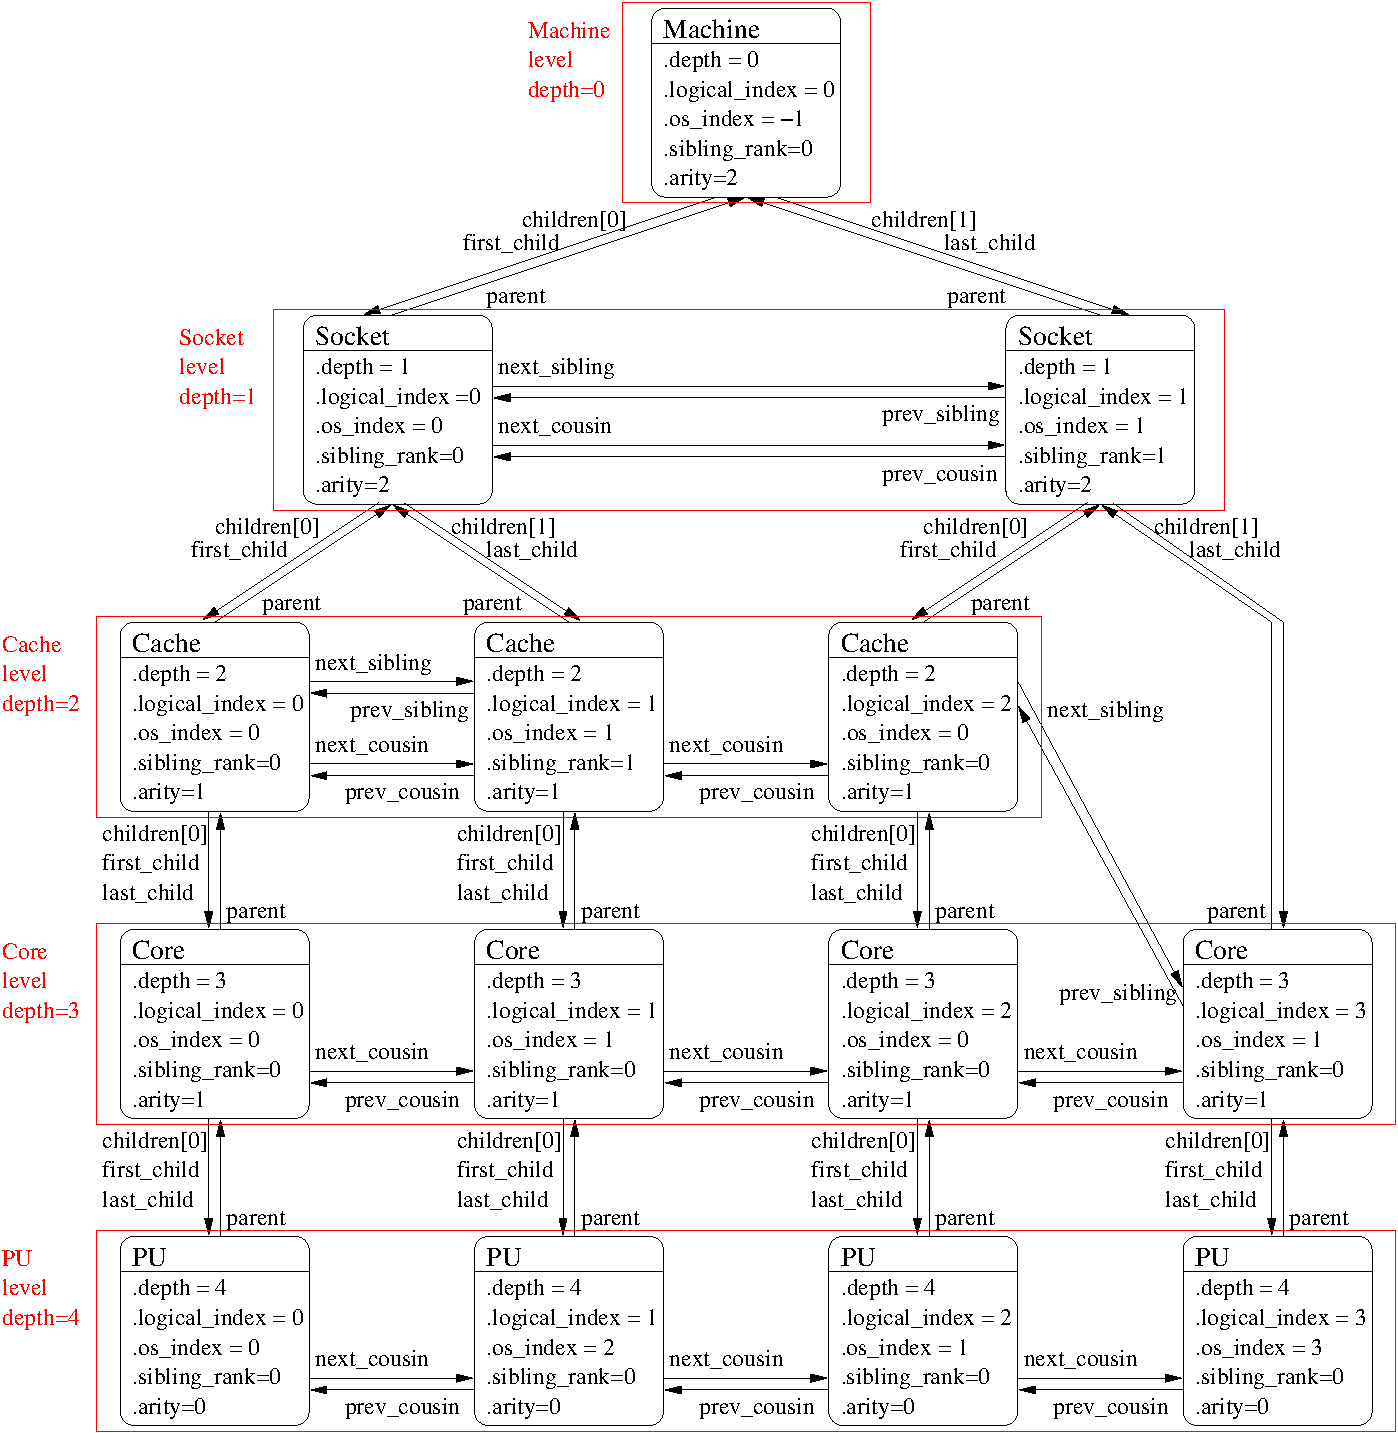
\includegraphics[width=\textwidth]{diagram}}
\end{DoxyImageNoCaption}


It should be noted that for PU objects, the logical index -\/-\/ as computed linearly by hwloc -\/-\/ is not the same as the OS index.

See also \hyperlink{a00011_faq_asymmetric}{What happens if my topology is asymmetric?} for more details. 
\chapter{Command-\/Line Tools}
\label{tools}
\hypertarget{tools}{}
hwloc comes with an extensive C programming interface and several command line utilities. Each of them is fully documented in its own manual page; the following is a summary of the available command line tools.\hypertarget{a00002_cli_lstopo}{}\section{lstopo}\label{a00002_cli_lstopo}
lstopo (also known as hwloc-\/info and hwloc-\/ls) displays the hierarchical topology map of the current system. The output may be graphical or textual, and can also be exported to numerous file formats such as PDF, PNG, XML, and others.

This command can also display the processes currently bound to a part of the machine (via the -\/-\/ps option).

Note that lstopo can read XML files and/or alternate chroot filesystems and display topological maps representing those systems (e.g., use lstopo to output an XML file on one system, and then use lstopo to read in that XML file and display it on a different system).\hypertarget{a00002_cli_hwloc_bind}{}\section{hwloc-\/bind}\label{a00002_cli_hwloc_bind}
hwloc-\/bind binds processes to specific hardware objects through a flexible syntax. A simple example is binding an executable to specific cores (or sockets or bitmaps or ...). The hwloc-\/bind(1) man page provides much more detail on what is possible.

hwloc-\/bind can also be used to retrieve the current process' binding.\hypertarget{a00002_cli_hwloc_calc}{}\section{hwloc-\/calc}\label{a00002_cli_hwloc_calc}
hwloc-\/calc is generally used to create bitmap strings to pass to hwloc-\/bind. Although hwloc-\/bind accepts many forms of object specification (i.e., bitmap strings are one of many forms that hwloc-\/bind understands), they can be useful, compact representations in shell scripts, for example.

hwloc-\/calc generates bitmap strings from given hardware objects with the ability to aggregate them, intersect them, and more. hwloc-\/calc generally uses the same syntax than hwloc-\/bind, but multiple instances may be composed to generate complex combinations.

Note that hwloc-\/calc can also generate lists of logical processors or NUMA nodes that are convenient to pass to some external tools such as taskset or numactl.\hypertarget{a00002_cli_hwloc_distrib}{}\section{hwloc-\/distrib}\label{a00002_cli_hwloc_distrib}
hwloc-\/distrib generates a set of bitmap strings that are uniformly distributed across the machine for the given number of processes. These strings may be used with hwloc-\/bind to run processes to maximize their memory bandwidth by properly distributing them across the machine.\hypertarget{a00002_cli_hwloc_ps}{}\section{hwloc-\/ps}\label{a00002_cli_hwloc_ps}
hwloc-\/ps is a tool to display the bindings of processes that are currently running on the local machine. By default, hwloc-\/ps only lists processes that are bound; unbound process (and Linux kernel threads) are not displayed.\hypertarget{a00002_cli_hwloc_gather}{}\section{hwloc-\/gather-\/topology}\label{a00002_cli_hwloc_gather}
hwloc-\/gather-\/topology is a Linux-\/specific tool that saves the relevant topology files of the current machine into a tarball (and the corresponding lstopo output). These files may be used later (possibly offline) for simulating or debugging a machine without actually running on it.\hypertarget{a00002_cli_hwloc_distances}{}\section{hwloc-\/distances}\label{a00002_cli_hwloc_distances}
hwloc-\/distances displays all distance matrices attached to the topology. Note that lstopo may also display distance matrices in its verbose textual output. However lstopo only prints matrices that cover the entire topology while hwloc-\/distances also displays matrices that ignore part of the topology.\hypertarget{a00002_cli_hwloc_assembler}{}\section{hwloc-\/assembler}\label{a00002_cli_hwloc_assembler}
hwloc-\/assembler combines several XML topology files into a single multi-\/node XML topology. It may then be used later as input with \hyperlink{a00044_ga93efcc8a962afe1ed23393700682173f}{hwloc\_\-topology\_\-set\_\-xml()} or with the HWLOC\_\-XMLFILE environment variable. See \hyperlink{a00006}{Multi-\/node Topologies} for details.\hypertarget{a00002_cli_hwloc_assembler_remote}{}\section{hwloc-\/assembler-\/remote}\label{a00002_cli_hwloc_assembler_remote}
hwloc-\/assembler-\/remote is a frontend to hwloc-\/assembler. It takes care of contacting the given list of remote hosts (through ssh) and retrieving their topologies as XML before assembling them with hwloc-\/assembler. 
\chapter{Environment Variables}
\label{envvar}
\hypertarget{envvar}{}
The behavior of the hwloc library and tools may be tuned thanks to the following environment variables.


\begin{DoxyDescription}
\item[HWLOC\_\-XMLFILE=/path/to/file.xml ]enforces the discovery from the given XML file as if \hyperlink{a00044_ga93efcc8a962afe1ed23393700682173f}{hwloc\_\-topology\_\-set\_\-xml()} had been called. This file may have been generated earlier with lstopo file.xml. For convenience, this backend provides empty binding hooks which just return success. To have hwloc still actually call OS-\/specific hooks, HWLOC\_\-THISSYSTEM should be set 1 in the environment too, to assert that the loaded file is really the underlying system. See also \hyperlink{a00007}{Importing and exporting topologies from/to XML files}. 


\item[HWLOC\_\-XML\_\-VERBOSE=1 ]
\item[HWLOC\_\-SYNTHETIC\_\-VERBOSE=1 ]enable verbose messages in the XML or synthetic topology backends. hwloc XML backends (see \hyperlink{a00007}{Importing and exporting topologies from/to XML files}) can emit some error messages to the error output stream. Enabling these verbose messages within hwloc can be useful for understanding failures to parse input XML topologies. Similarly, enabling verbose messages in the synthetic topology backend can help understand why the description string is invalid. 


\item[HWLOC\_\-FSROOT=/path/to/linux/filesystem-\/root/ ]switches to reading the topology from the specified Linux filesystem root instead of the main file-\/system root, as if \hyperlink{a00044_ga2f6bfb6958d8b508ea1d7d5bb266432c}{hwloc\_\-topology\_\-set\_\-fsroot()} had been called. Not using the main file-\/system root causes \hyperlink{a00046_ga0d109e33fc7990f62f665d336e5e5111}{hwloc\_\-topology\_\-is\_\-thissystem()} to return 0. For convenience, this backend provides empty binding hooks which just return success. To have hwloc still actually call OS-\/specific hooks, HWLOC\_\-THISSYSTEM should be set 1 in the environment too, to assert that the loaded file is really the underlying system. 


\item[HWLOC\_\-THISSYSTEM=1 ]enforces the return value of \hyperlink{a00046_ga0d109e33fc7990f62f665d336e5e5111}{hwloc\_\-topology\_\-is\_\-thissystem()}, as if HWLOC\_\-TOPOLOGY\_\-FLAG\_\-IS\_\-THISSYSTEM was set with \hyperlink{a00044_ga6d11e53db143ac39c32cdb3912b71f99}{hwloc\_\-topology\_\-set\_\-flags()}. It means that it makes hwloc assume that the selected backend provides the topology for the system on which we are running, even if it is not the OS-\/specific backend but the XML backend for instance. This means making the binding functions actually call the OS-\/specific system calls and really do binding, while the XML backend would otherwise provide empty hooks just returning success. This can be used for efficiency reasons to first detect the topology once, save it to an XML file, and quickly reload it later through the XML backend, but still having binding functions actually do bind. 


\item[HWLOC\_\-HIDE\_\-ERRORS=0 ]enables or disables verbose reporting of errors. The hwloc library may issue warnings to the standard error stream when it detects a problem during topology discovery, for instance if the operating system (or user) gives contradictory topology information. Setting this environment variable to 1 removes the actual displaying of these error messages. 


\item[HWLOC\_\-GROUPING=1 ]enables or disables objects grouping based on distances. By default, hwloc uses distance matrices between objects (either read from the OS or given by the user) to find groups of close objects. These groups are described by adding intermediate Group objects in the topology. Setting this environment variable to 0 will disable this grouping. This variable supersedes the obsolete HWLOC\_\-IGNORE\_\-DISTANCES variable. 


\item[HWLOC\_\-GROUPING\_\-ACCURACY=0.05 ]relaxes distance comparison during grouping. By default, objects may be grouped if their distances form a minimal distance graph. When setting this variable to 0.02, these distances do not have to be strictly equal anymore, they may just be equal with a 2\% error. If set to {\ttfamily try} instead of a numerical value, hwloc will try to group with perfect accuracy (0, the default), then with 0.01, 0.02, 0.05 and finally 0.1.


\item[HWLOC\_\-GROUPING\_\-VERBOSE=0 ]enables or disables some verbose messages during grouping. If this variable is set to 1, some debug messages will be displayed during distance-\/based grouping of objects even if debug was not specific at configure time. This is useful when trying to find an interesting distance grouping accuracy.


\item[HWLOC\_\-$<$type$>$\_\-DISTANCES=index,...:X$\ast$Y ]
\item[HWLOC\_\-$<$type$>$\_\-DISTANCES=begin-\/end:X$\ast$Y$\ast$Z ]
\item[HWLOC\_\-$<$type$>$\_\-DISTANCES=index,...:distance,... ]sets a distance matrix for objects of the given type and physical indexes. The type should be given as its case-\/sensitive stringified value (e.g. {\ttfamily NUMANode}, {\ttfamily Socket}, {\ttfamily Cache}, {\ttfamily Core}, {\ttfamily PU}). If another distance matrix already exists for the given type, either because the user specified it or because the OS offers it, it will be replaced by the given one.

If the variable value is {\ttfamily none}, the existing distance matrix for the given type is removed. Otherwise, the variable value first consists in a list of physical indexes that may be specified as a comma-\/separated list (e.g. {\ttfamily 0,2,4,1,3,5}) or as a range of consecutive indexes ({\ttfamily 0-\/5}). It is followed by a colon and the corresponding distances: 
\begin{DoxyItemize}
\item If {\ttfamily X$\ast$Y} is given, X groups of Y close objects are specified. 
\item If {\ttfamily X$\ast$Y$\ast$Z} is given, X groups of Y groups of Z close objects are specified. 
\item Otherwise, the comma-\/separated list of distances should be given. If N objects are considered, the i$\ast$N+j-\/th value gives the distance from the i-\/th object to the j-\/th object. These distance values must use a dot as a decimal separator. 
\end{DoxyItemize}

Note that distances are ignored in multi-\/node topologies. 


\item[HWLOC\_\-PCI\_\-$<$domain$>$\_\-$<$bus$>$\_\-LOCALCPUS=$<$cpuset$>$ ]changes the locality of I/O devices behind the specified PCI hostbridge. If no I/O locality information is available or if the BIOS reports incorrect information, it is possible to move a I/O device tree (the entire set of objects behind a host bridge) near a custom set of processors. {\ttfamily domain} and {\ttfamily bus} are the PCI domain and primary bus of the corresponding host bridge. 


\end{DoxyDescription}
\chapter{CPU and Memory Binding Overview}
\label{cpu_mem_bind}
\hypertarget{cpu_mem_bind}{}
Some operating systems do not systematically provide separate functions for CPU and memory binding. This means that CPU binding functions may have have effects on the memory binding policy. Likewise, changing the memory binding policy may change the CPU binding of the current thread. This is often not a problem for applications, so by default hwloc will make use of these functions when they provide better binding support.

If the application does not want the CPU binding to change when changing the memory policy, it needs to use the HWLOC\_\-MEMBIND\_\-NOCPUBIND flag to prevent hwloc from using OS functions which would change the CPU binding. Additionally, HWLOC\_\-CPUBIND\_\-NOMEMBIND can be passed to CPU binding function to prevent hwloc from using OS functions would change the memory binding policy. Of course, using these flags will reduce hwloc's overall support for binding, so their use is discouraged.

One can avoid using these flags but still closely control both memory and CPU binding by allocating memory, touching each page in the allocated memory, and then changing the CPU binding. The already-\/really-\/allocated memory will then be \char`\"{}locked\char`\"{} to physical memory and will not be migrated. Thus, even if the memory binding policy gets changed by the CPU binding order, the already-\/allocated memory will not change with it. When binding and allocating further memory, the CPU binding should be performed again in case the memory binding altered the previously-\/selected CPU binding.

Not all operating systems support the notion of a \char`\"{}current\char`\"{} memory binding policy for the current process, but such operating systems often still provide a way to allocate data on a given node set. Conversely, some operating systems support the notion of a \char`\"{}current\char`\"{} memory binding policy and do not permit allocating data on a specific node set without changing the current policy and allocate the data. To provide the most powerful coverage of these facilities, hwloc provides:


\begin{DoxyItemize}
\item functions that set/get the current memory binding policies (if supported): hwloc\_\-set/get\_\-membind\_\-$\ast$() and hwloc\_\-set/get\_\-proc\_\-membind() 
\item functions that allocate memory bound to specific node set without changing the current memory binding policy (if supported): \hyperlink{a00050_ga221a7edc5d436300374fa16463f607e5}{hwloc\_\-alloc\_\-membind()} and \hyperlink{a00050_gaeaa00714a9c4319bda0a74ca6f8720e8}{hwloc\_\-alloc\_\-membind\_\-nodeset()}. 
\item helpers which, if needed, change the current memory binding policy of the process in order to obtain memory binding: \hyperlink{a00059_ga6178c6a9ec1dd88ec9f6a9fcdcc7d634}{hwloc\_\-alloc\_\-membind\_\-policy()} and \hyperlink{a00059_ga3e772fbc4de626ed80f13d332b7d4d03}{hwloc\_\-alloc\_\-membind\_\-policy\_\-nodeset()} 
\end{DoxyItemize}

An application can thus use the two first sets of functions if it wants to manage separately the global process binding policy and directed allocation, or use the third set of functions if it does not care about the process memory binding policy.

See \hyperlink{a00049}{CPU binding} and \hyperlink{a00050}{Memory binding} for hwloc's API functions regarding CPU and memory binding, respectively. 
\chapter{I/O Devices}
\label{iodevices}
\hypertarget{iodevices}{}
hwloc usually manipulates processing units and memory but it can actually discover I/O devices and report their locality as well. This is useful for placing I/O intensive applications on cores near the I/O devices they use.\hypertarget{a00005_iodevices_enabling}{}\section{Enabling and requirements}\label{a00005_iodevices_enabling}
I/O discovery is disabled by default (except in lstopo) so as not to break legacy application by adding unexpected I/O objects to the topology. It can be enabled by passing flags such as {\ttfamily \hyperlink{a00044_ggada025d3ec20b4b420f8038d23d6e7bdea46ae25e8896278840b1800ae9ce4de41}{HWLOC\_\-TOPOLOGY\_\-FLAG\_\-IO\_\-DEVICES}} to \hyperlink{a00044_ga6d11e53db143ac39c32cdb3912b71f99}{hwloc\_\-topology\_\-set\_\-flags()} before loading the topology.

Note that I/O discovery requires significant help from the operating system. The pciutils library is needed to detect PCI devices and bridges, and the actual locality of these devices is only currently detected on Linux. Also, some operating systems require privileges for probing PCI devices, see \hyperlink{a00011_faq_privileged}{Does hwloc require privileged access?} for details.\hypertarget{a00005_iodevices_hierarchy}{}\section{I/O object hierarchy}\label{a00005_iodevices_hierarchy}
When I/O discovery is enabled and supported, some additional objects (types {\ttfamily \hyperlink{a00041_ggacd37bb612667dc437d66bfb175a8dc55a6825f10895fea60aca7a6ba9fe273db0}{HWLOC\_\-OBJ\_\-BRIDGE}}, {\ttfamily \hyperlink{a00041_ggacd37bb612667dc437d66bfb175a8dc55a5d8117a54df1fbd3606ab19e42cb0ea9}{HWLOC\_\-OBJ\_\-PCI\_\-DEVICE}} and {\ttfamily \hyperlink{a00041_ggacd37bb612667dc437d66bfb175a8dc55a51e7280240fd9f25589cbbe538bdb075}{HWLOC\_\-OBJ\_\-OS\_\-DEVICE}}) are added to the topology as a child of the object they are close to. For instance, if a I/O Hub is connected to a socket, the corresponding hwloc bridge object (and its PCI bridges and devices children) is inserted as a child of the corresponding hwloc socket object.

These new objects have neither CPU sets nor node sets (NULL pointers) because they are not directly usable by the user applications. Moreover I/O hierarchies may be highly complex (asymmetric trees of bridges). So I/O objects are placed in specific levels with custom depths. Their lists may still be traversed with regular helpers such as \hyperlink{a00053_ga5f08ceb69375341e73563cfe2e77534e}{hwloc\_\-get\_\-next\_\-obj\_\-by\_\-type()}. However, hwloc offers some dedicated helpers such as \hyperlink{a00064_gad6e1ed122ef3b6e098538d75acd5e3f6}{hwloc\_\-get\_\-next\_\-pcidev()} and \hyperlink{a00064_ga73a5bc6265642e6001f7a10812ab886d}{hwloc\_\-get\_\-next\_\-osdev()} for convenience (see \hyperlink{a00064}{Advanced I/O object traversal helpers}).

An I/O hierarchy is organized as follows: A hostbridge object ( {\ttfamily \hyperlink{a00041_ggacd37bb612667dc437d66bfb175a8dc55a6825f10895fea60aca7a6ba9fe273db0}{HWLOC\_\-OBJ\_\-BRIDGE}} object with upstream type {\itshape Host\/} and downstream type {\itshape PCI\/}) is attached below a regular object (usually the entire machine or a NUMA node). There may be multiple hostbridges in the machine, attached to different places, but all I/O devices are below one of them. Each hostbridge contains one or several children, either other bridges (usually PCI to PCI) or PCI devices ({\ttfamily \hyperlink{a00041_ggacd37bb612667dc437d66bfb175a8dc55a5d8117a54df1fbd3606ab19e42cb0ea9}{HWLOC\_\-OBJ\_\-PCI\_\-DEVICE}}). The number of bridges between the hostbridge and a PCI device depends on the machine and on the topology flags.\hypertarget{a00005_iodevices_osdev}{}\section{Software devices}\label{a00005_iodevices_osdev}
Although each PCI device is uniquely identified by its bus ID (e.g. 0000:01:02.3), the application can hardly find out which PCI device is actually used when manipulating software handle (such as the {\itshape eth0\/} network interface or the {\itshape mlx4\_\-0\/} OpenFabrics HCA). Therefore hwloc tries to add software devices ({\ttfamily \hyperlink{a00041_ggacd37bb612667dc437d66bfb175a8dc55a51e7280240fd9f25589cbbe538bdb075}{HWLOC\_\-OBJ\_\-OS\_\-DEVICE}}) below their PCI objects. These objects can be identified by their usual operating system-\/wide names, e.g. {\itshape eth0\/} or {\itshape mlx4\_\-0\/}. However, this ability is currently only available on Linux for some classes of devices. It should especially be noted that proprietary graphics driver currently do not create any interesting software device for GPUs, they should therefore be manipulated as PCI device objects. On the contrary some PCI devices may contain multiple software device (see the example below).

See also \hyperlink{a00008}{Interoperability With Other Software} for managing these devices without considering them as hwloc objects.\hypertarget{a00005_iodevices_consult}{}\section{Consulting I/O devices and binding}\label{a00005_iodevices_consult}
I/O devices may be consulted by traversing the topology manually (with usual routines such as \hyperlink{a00047_ga9be4a03488cdd0fb431e4aa1cbdea895}{hwloc\_\-get\_\-obj\_\-by\_\-type()}) or by using dedicated helpers (such as \hyperlink{a00064_ga546e1d690c63fb24177f3013ed78ceb1}{hwloc\_\-get\_\-pcidev\_\-by\_\-busid()}, see \hyperlink{a00064}{Advanced I/O object traversal helpers}).

I/O objects do not actually contain any locality information because their CPU sets and node sets are NULL. Their locality must be retrieved by walking up the object tree (through the {\ttfamily parent} link) until an non-\/I/O object is found (see \hyperlink{a00064_ga3603275746a8792e54415d79763aa9e9}{hwloc\_\-get\_\-non\_\-io\_\-ancestor\_\-obj()}). This regular object should have non-\/NULL CPU sets and node sets which describe the processing units and memory that are immediately close to the I/O device. For instance the path from a OS device to its locality may go across a PCI device parent, one or several bridges, up to a a NUMA node with the same locality.

Command-\/line tools are also aware of I/O devices. lstopo displays the interesting ones by default (passing {\ttfamily -\/-\/no-\/io} disables it).

hwloc-\/calc and hwloc-\/bind may manipulate I/O devices specified by PCI bus ID or by OS device name. For instance, {\ttfamily pci=0000:02:03.0} (respectively {\ttfamily os=eth0}) is replaced by the set of CPUs that are close to this PCI device (respectively software device). This enables easy binding of I/O-\/intensive applications near the device they use.\hypertarget{a00005_iodevices_examples}{}\section{Examples}\label{a00005_iodevices_examples}
The following picture shows a dual-\/socket dual-\/core host whose PCI bus is connected to the first socket and NUMA node.

 
\begin{DoxyImageNoCaption}
  \mbox{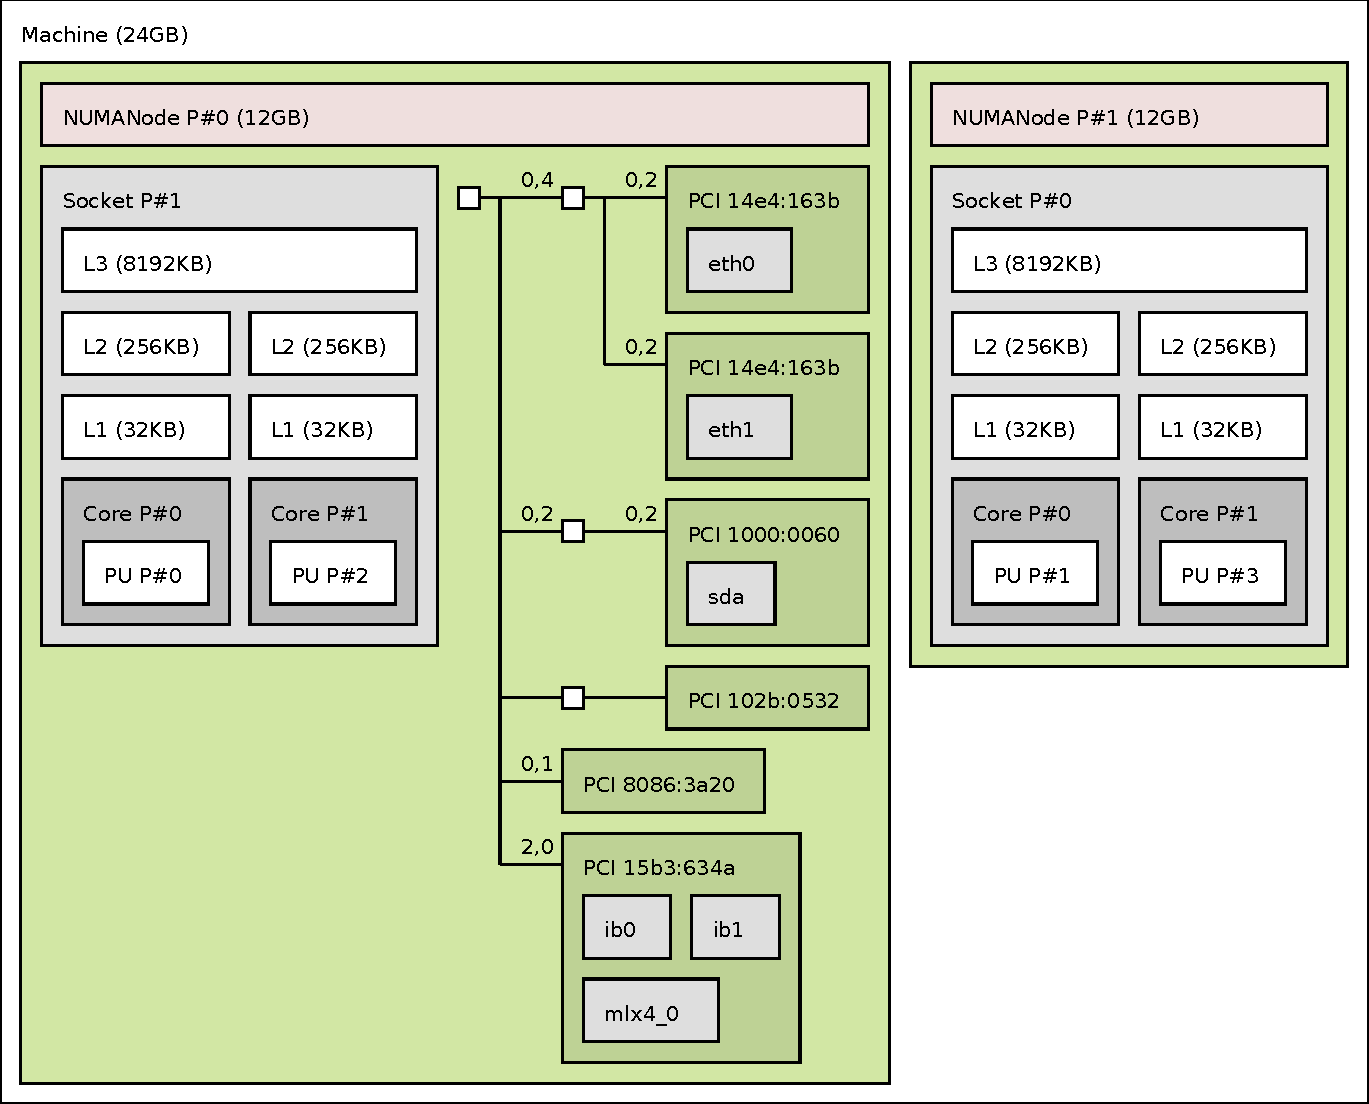
\includegraphics[width=\textwidth]{devel09-pci}}
\end{DoxyImageNoCaption}


Six interesting PCI devices were discovered. However hwloc found some corresponding software devices ({\itshape eth0\/}, {\itshape eth1\/}, {\itshape sda\/}, {\itshape mlx4\_\-0\/}, {\itshape ib0\/}, and {\itshape ib1\/}) for only four of these physical devices. The other ones ({\itshape PCI 102b:0532\/} and {\itshape PCI 8086:3a20\/}) are an unused IDE controller (no disk attached) and a graphic card (no corresponding software device reported to the user by the operating system).

On the contrary, it should be noted three different software devices were found for the last PCI device ({\itshape PCI 15b3:634a\/}). Indeed this OpenFabrics HCA PCI device object contains one one OpenFabrics software device ({\itshape mlx4\_\-0\/}) and two virtual network interface software devices ({\itshape ib0\/} and {\itshape ib1\/}).

PCI link speed is also reported for some bridges and devices because lstopo was privileged when it discovered the topology.

Here is the corresponding textual output:

\begin{DoxyVerb}
Machine (24GB)
  NUMANode L#0 (P#0 12GB)
    Socket L#0 + L3 L#0 (8192KB)
      L2 L#0 (256KB) + L1 L#0 (32KB) + Core L#0 + PU L#0 (P#0)
      L2 L#1 (256KB) + L1 L#1 (32KB) + Core L#1 + PU L#1 (P#2)
    HostBridge
      PCIBridge
        PCI 14e4:163b
          Net "eth0"
        PCI 14e4:163b
          Net "eth1"
      PCIBridge
        PCI 1000:0060
          Block "sda"
      PCIBridge
        PCI 102b:0532
      PCI 8086:3a20
      PCI 15b3:634a
        Net "ib0"
        Net "ib1"
        Net "mlx4_0"
  NUMANode L#1 (P#1 12GB) + Socket L#1 + L3 L#1 (8192KB)
    L2 L#2 (256KB) + L1 L#2 (32KB) + Core L#2 + PU L#2 (P#1)
    L2 L#3 (256KB) + L1 L#3 (32KB) + Core L#3 + PU L#3 (P#3)
\end{DoxyVerb}
 
\chapter{Multi-\/node Topologies}
\label{multinode}
\hypertarget{multinode}{}
hwloc is usually used for consulting and manipulating single machine topologies. This includes large systems as long as a single instance of the operating system manages the entire system. However it is sometimes desirable to have multiple independent hosts inside the same topology, for instance when applying algorithms to an entire cluster topology. hwloc therefore offers the ability to agregate multiple host topologies into a single global one.\hypertarget{a00006_multinode_cpusets}{}\section{Multi-\/node Objects Specifities}\label{a00006_multinode_cpusets}
A multi-\/node topology contains several single-\/node topologies. Those are assembled by making their own root objects (usually Machine object) children of higher objects. These higher objects include at least the root of the global topology (usually a System object). Some intermediate objects may also exists, for instance to represent switches in a large fabric.

There are actually three possible types of objects that have different properties with respect to cpusets, nodesets and binding. Indeed those cpusets and nodesets were designed for execution and memory binding within a single operating system. Binding on another system or across several different systems would be meaningless.


\begin{DoxyDescription}
\item[Local objects ]Any object that corresponds to the local machine may be manipulated as usual. Obviously, if the multi-\/node topology does not contain the local machine topology, no such local object exists.  
\item[Objects from other nodes ]Any object that comes from inside another node is represented as usual but its cpusets and nodesets should not be used for binding since binding on another system makes no sense.  
\item[Objects above single nodes ]Any object above single-\/node topologies does not have any cpuset or nodeset pointer because binding across multiple systems makes no sense. This includes the glocal root object of a multi-\/node topology and possibly some intermediate objects between this global root and the local root of single-\/node topologies.  
\end{DoxyDescription}

It is important to keep this in mind before binding using multi-\/node topologies. To make sure binding on an object is possible, one should first check that its cpuset or nodeset pointer is not NULL. Then, one should check whether the object is indeed local.

To find out which machine a given object correspond too, one may look at the info attributes of the parent Machine object. The {\ttfamily HostName} info is usually available in Machine objects, it may be retrieved with the following code: \begin{DoxyVerb}
  hwloc_obj_t machine_obj;
  obj = hwloc_get_ancestor_obj_by_type(topology, HWLOC_OBJ_MACHINE, obj);
  if (machine_obj)
    return hwloc_obj_get_info_by_name(machine_obj, "HostName");
  else
    return NULL;
\end{DoxyVerb}
 The hwloc assembler scripts (see below) also add {\ttfamily AssemblerName} and {\ttfamily AssemblerIndex} info attributes to the Machine objects to identify the corresponding host name and index during assembly.\hypertarget{a00006_multinode_tools}{}\section{Assembling topologies with command-\/line tools}\label{a00006_multinode_tools}
One way to manipulate multinode topologies is to retrieve other nodes' topologies as XML files and combine them as a global XML topology. It may then be loaded with \hyperlink{a00044_ga93efcc8a962afe1ed23393700682173f}{hwloc\_\-topology\_\-set\_\-xml()} or with the HWLOC\_\-XMLFILE environment variable.

The hwloc-\/assembler and hwloc-\/assembler-\/remote utilities offer the ability to combine XML topologies or remote nodes' topologies (see \hyperlink{a00002}{Command-\/Line Tools}).\hypertarget{a00006_multinode_interface}{}\section{Assembling topologies with the programming interface}\label{a00006_multinode_interface}
The hwloc programming interface offers the ability to build multinode topologies using the {\itshape custom\/} interface. A new multinode topology has to be initialized with \hyperlink{a00043_ga5c2d6f476af87005c7bd0811d4548b9f}{hwloc\_\-topology\_\-init()} and then set to custom with \hyperlink{a00044_ga12024fec46f9368fb8fc5c624089c5ec}{hwloc\_\-topology\_\-set\_\-custom()}. Topologies and objects mat then be assembled. Later, the custom topology is finalized as usual with \hyperlink{a00043_ga91e2e6427b95fb7339c99dbbef996e71}{hwloc\_\-topology\_\-load()}.

A custom topology starts with a single root object of type System. It may be modified by inserting a new child object with \hyperlink{a00051_gac1037fe389bfa7c2bf0e3739b7e20844}{hwloc\_\-custom\_\-insert\_\-group\_\-object\_\-by\_\-parent()} or by duplicating another topology with \hyperlink{a00051_ga59ccf6a63cb23d63940e8b782059d9cb}{hwloc\_\-custom\_\-insert\_\-topology()}. Both of these operations require to specify the parent object in the custom topology where the insertion will take place. This parent may be either the root (returned by \hyperlink{a00053_gadbf58f6e187efbdb3cd9a8e30311b7d7}{hwloc\_\-get\_\-root\_\-obj()}) or an already-\/inserted object (returned by \hyperlink{a00051_gac1037fe389bfa7c2bf0e3739b7e20844}{hwloc\_\-custom\_\-insert\_\-group\_\-object\_\-by\_\-parent()}).

Ideally, any existing object in the custom topology could be the parent. However, special care should be taken when traversing the topology to find such an object because most links between objects (children, siblings, cousins) are not setup until \hyperlink{a00043_ga91e2e6427b95fb7339c99dbbef996e71}{hwloc\_\-topology\_\-load()} is invoked.\hypertarget{a00006_multinode_example}{}\section{Example of assembly with the programming interface}\label{a00006_multinode_example}
If the topologies of two hosts have been previously gathered in XML files {\ttfamily host1.xml} and {\ttfamily host2.xml}, the global topology may be assembled with the following code.

\begin{DoxyVerb}
hwloc_topology_t host1, host2, global;

/* initialize global topology */
hwloc_topology_init(&global);
hwloc_topology_set_custom(global);

/* insert host1 entire topology below the global topology root */
hwloc_topology_init(&host1);
hwloc_topology_load(host1);
hwloc_custom_insert_topology(global, hwloc_get_root_obj(global),
                             host1, NULL);
hwloc_topology_destroy(host1);

/* insert host2 entire topology below the global topology root */
hwloc_topology_init(&host2);
hwloc_topology_load(host2);
hwloc_custom_insert_topology(global, hwloc_get_root_obj(global),
                             host2, NULL);
hwloc_topology_destroy(host2);

/* load and play with the global topology */
hwloc_topology_load(global);
...
\end{DoxyVerb}


If a intermediate object such as a switch should be inserted above one of the host topologies: \begin{DoxyVerb}
...
/* insert a switch object below the global topology root */
hwloc_obj_t sw =
   hwloc_custom_insert_group_object_by_parent(global,
                              hwloc_get_root_obj(global), 0);

/* insert host2 entire topology below the switch */
hwloc_topology_init(&host2);
hwloc_topology_load(host2);
hwloc_custom_insert_topology(global, switch, host2, NULL);
hwloc_topology_destroy(host2);

/* load and play with the global topology */
hwloc_topology_load(global);
...
\end{DoxyVerb}
 
\chapter{Importing and exporting topologies from/to XML files}
\label{xml}
\hypertarget{xml}{}
hwloc offers the ability to export topologies to XML files and reload them later. This is for instance useful for loading topologies faster (see \hyperlink{a00011_faq_xml}{I do not want hwloc to rediscover my enormous machine topology every time I rerun a process}), manipulating other nodes' topology, or avoiding the need for privileged processes (see \hyperlink{a00011_faq_privileged}{Does hwloc require privileged access?}).

Topologies may be exported to XML files thanks to \hyperlink{a00045_ga45578d725c66865cfef31d0585dcff70}{hwloc\_\-topology\_\-export\_\-xml()}, or to a XML memory buffer with \hyperlink{a00045_ga739330e9402425315e44e5012631fb91}{hwloc\_\-topology\_\-export\_\-xmlbuffer()}. The lstopo program can also serve as a XML topology export tool.

XML topologies may then be reloaded later with \hyperlink{a00044_ga93efcc8a962afe1ed23393700682173f}{hwloc\_\-topology\_\-set\_\-xml()} and \hyperlink{a00044_gae7e4bade144652a2b48f5eaf0309b4ec}{hwloc\_\-topology\_\-set\_\-xmlbuffer()}. The XMLFILE environment variable also tells hwloc to load the topology from the given XML file.

\begin{DoxyNote}{Note}
Loading XML topologies disables binding because the loaded topology may not correspond to the physical machine that loads it. This behavior may be reverted by asserting that loaded file really matches the underlying system with the HWLOC\_\-THISSYSTEM environment variable or the HWLOC\_\-TOPOLOGY\_\-FLAG\_\-IS\_\-THISSYSTEM topology flag.

XML topology files are not localized. They use a dot as a decimal separator. Therefore any exported topology can be reloaded on any other machine without requiring to change the locale.
\end{DoxyNote}
\hypertarget{a00007_xml_backends}{}\section{libxml2 and minimalistic XML backends}\label{a00007_xml_backends}
hwloc offers two backends for importing/exporting XML.

First, it can use the libxml2 library for importing/exporting XML files. It features full XML support, for instance when those files have to be manipulated by non-\/hwloc software (e.g. a XSLT parser). The libxml2 backend is enabled by default if libxml2 development headers are available.

If libxml2 is not available at configure time, or if {\ttfamily -\/-\/disable-\/libxml2} is passed, hwloc falls back to a custom backend. Contrary to the aforementioned full XML backend with libxml2, this minimalistic XML backend cannot be guaranteed to work with external programs. It should only be assumed to be compatible with the same hwloc release (even if using the libxml2 backend). Its advantage is however to always be available without requiring any external dependency.\hypertarget{a00007_xml_errors}{}\section{XML import error management}\label{a00007_xml_errors}
Importing XML files can fail at least because of file access errors, invalid XML syntax or non-\/hwloc-\/valid XML contents.

Both backend cannot detect all these errors when the input XML file or buffer is selected (when \hyperlink{a00044_ga93efcc8a962afe1ed23393700682173f}{hwloc\_\-topology\_\-set\_\-xml()} or \hyperlink{a00044_gae7e4bade144652a2b48f5eaf0309b4ec}{hwloc\_\-topology\_\-set\_\-xmlbuffer()} is called). Some errors such non-\/hwloc-\/valid contents can only be detected later when loading the topology with \hyperlink{a00043_ga91e2e6427b95fb7339c99dbbef996e71}{hwloc\_\-topology\_\-load()}.

It is therefore strongly recommended to check the return value of both \hyperlink{a00044_ga93efcc8a962afe1ed23393700682173f}{hwloc\_\-topology\_\-set\_\-xml()} (or \hyperlink{a00044_gae7e4bade144652a2b48f5eaf0309b4ec}{hwloc\_\-topology\_\-set\_\-xmlbuffer()}) and \hyperlink{a00043_ga91e2e6427b95fb7339c99dbbef996e71}{hwloc\_\-topology\_\-load()} to handle all these errors. 
\chapter{Interoperability With Other Software}
\label{interoperability}
\hypertarget{interoperability}{}
Although hwloc offers its own portable interface, it still may have to interoperate with specific or non-\/portable libraries that manipulate similar kinds of objects. hwloc therefore offers several specific \char`\"{}helpers\char`\"{} to assist converting between those specific interfaces and hwloc.

Some external libraries may be specific to a particular OS; others may not always be available. The hwloc core therefore generally does not explicitly depend on these types of libraries. However, when a custom application uses or otherwise depends on such a library, it may optionally include the corresponding hwloc helper to extend the hwloc interface with dedicated helpers.

Most of these helpers use structures that are specific to these external libraries and only meaningful on the local machine. If so, the helper requires the input topology to match the current machine. Some helpers also require I/O device discovery to be supported and enabled for the current topology.


\begin{DoxyDescription}
\item[Linux specific features ]\hyperlink{a00035_source}{hwloc/linux.h} offers Linux-\/specific helpers that utilize some non-\/portable features of the Linux system, such as binding threads through their thread ID (\char`\"{}tid\char`\"{}) or parsing kernel CPU mask files. 


\item[Linux libnuma ]\hyperlink{a00034_source}{hwloc/linux-\/libnuma.h} provides conversion helpers between hwloc CPU sets and libnuma-\/specific types, such as bitmasks. It helps you use libnuma memory-\/binding functions with hwloc CPU sets. 


\item[Glibc ]\hyperlink{a00030_source}{hwloc/glibc-\/sched.h} offers conversion routines between Glibc and hwloc CPU sets in order to use hwloc with functions such as sched\_\-setaffinity(). 


\item[OpenFabrics Verbs ]\hyperlink{a00037_source}{hwloc/openfabrics-\/verbs.h} helps interoperability with the OpenFabrics Verbs interface. For example, it can return a list of processors near an OpenFabrics device. Note that if I/O device discovery is enabled, such devices may also appear as PCI objects and as OS objects in the topology. 


\item[Myrinet Express ]\hyperlink{a00036_source}{hwloc/myriexpress.h} offers interoperability with the Myrinet Express interface. It can return the list of processors near a Myrinet board managed by the MX driver. Note that if I/O device discovery is enabled, such boards may also appear as PCI objects in the topology. 


\item[NVIDIA CUDA ]\hyperlink{a00028_source}{hwloc/cuda.h} and \hyperlink{a00029_source}{hwloc/cudart.h} enable interoperability with NVIDIA CUDA Driver and Runtime interfaces. For instance, it may return the list of processors near NVIDIA GPUs. Note that if I/O device discovery is enabled, GPUs may also appear as PCI objects in the topology. 


\item[Taskset command-\/line tool ]The taskset command-\/line tool is widely used for binding processes. It manipulates CPU set strings in a format that is slightly different from hwloc's one (it does not divide the string in fixed-\/size subsets and separates them with commas). To ease interoperability, hwloc offers routines to convert hwloc CPU sets from/to taskset-\/specific string format. Most hwloc command-\/line tools also support the -\/-\/taskset option to manipulate taskset-\/specific strings. 


\end{DoxyDescription}
\chapter{Thread Safety}
\label{threadsafety}
\hypertarget{threadsafety}{}
Like most libraries that mainly fill data structures, hwloc is not thread safe but rather reentrant: all state is held in a \hyperlink{a00039_ga9d1e76ee15a7dee158b786c30b6a6e38}{hwloc\_\-topology\_\-t} instance without mutex protection. That means, for example, that two threads can safely operate on and modify two different \hyperlink{a00039_ga9d1e76ee15a7dee158b786c30b6a6e38}{hwloc\_\-topology\_\-t} instances, but they should not simultaneously invoke functions that modify the {\itshape same\/} instance. Similarly, one thread should not modify a \hyperlink{a00039_ga9d1e76ee15a7dee158b786c30b6a6e38}{hwloc\_\-topology\_\-t} instance while another thread is reading or traversing it. However, two threads can safely read or traverse the same \hyperlink{a00039_ga9d1e76ee15a7dee158b786c30b6a6e38}{hwloc\_\-topology\_\-t} instance concurrently.

When running in multiprocessor environments, be aware that proper thread synchronization and/or memory coherency protection is needed to pass hwloc data (such as \hyperlink{a00039_ga9d1e76ee15a7dee158b786c30b6a6e38}{hwloc\_\-topology\_\-t} pointers) from one processor to another (e.g., a mutex, semaphore, or a memory barrier). Note that this is not a hwloc-\/specific requirement, but it is worth mentioning.

For reference, \hyperlink{a00039_ga9d1e76ee15a7dee158b786c30b6a6e38}{hwloc\_\-topology\_\-t} modification operations include (but may not be limited to):


\begin{DoxyDescription}
\item[Creation and destruction ]{\ttfamily \hyperlink{a00043_ga5c2d6f476af87005c7bd0811d4548b9f}{hwloc\_\-topology\_\-init()}, \hyperlink{a00043_ga91e2e6427b95fb7339c99dbbef996e71}{hwloc\_\-topology\_\-load()}, \hyperlink{a00043_ga6040925d3ee4bbb2647f2a321aca5f4b}{hwloc\_\-topology\_\-destroy()}} (see \hyperlink{a00043}{Create and Destroy Topologies}) imply major modifications of the structure, including freeing some objects. No other thread cannot access the topology or any of its objects at the same time.

Also references to objects inside the topology are not valid anymore after these functions return. 


\item[Runtime topology modifications ]{\ttfamily hwloc\_\-topology\_\-insert\_\-misc\_\-object\_\-by\_\-$\ast$} (see \hyperlink{a00045}{Tinker With Topologies.}) may modify the topology significantly by adding objects inside the tree, changing the topology depth, etc. {\ttfamily hwloc\_\-topology\_\-restrict} modifies the topology even more dramatically by removing some objects.

Although references to former objects {\itshape may\/} still be valid after insertion or restriction, it is strongly advised to not rely on any such guarantee and always re-\/consult the topology to reacquire new instances of objects. 


\item[Locating topologies  ]{\ttfamily hwloc\_\-topology\_\-ignore$\ast$}, {\ttfamily hwloc\_\-topology\_\-set$\ast$} (see \hyperlink{a00044}{Configure Topology Detection}) do not modify the topology directly, but they do modify internal structures describing the behavior of the next invocation of {\ttfamily \hyperlink{a00043_ga91e2e6427b95fb7339c99dbbef996e71}{hwloc\_\-topology\_\-load()}}. Hence, all of these functions should not be used concurrently.

Note that these functions do not modify the current topology until it is actually reloaded; it is possible to use them while other threads are only read the current topology. 


\end{DoxyDescription}
\chapter{Embedding hwloc in Other Software}
\label{embed}
\hypertarget{embed}{}
It can be desirable to include hwloc in a larger software package (be sure to check out the LICENSE file) so that users don't have to separately download and install it before installing your software. This can be advantageous to ensure that your software uses a known-\/tested/good version of hwloc, or for use on systems that do not have hwloc pre-\/installed.

When used in \char`\"{}embedded\char`\"{} mode, hwloc will:


\begin{DoxyItemize}
\item not install any header files
\item not build any documentation files
\item not build or install any executables or tests
\item not build {\ttfamily libhwloc.$\ast$} -\/-\/ instead, it will build {\ttfamily libhwloc\_\-embedded.$\ast$}
\end{DoxyItemize}

There are two ways to put hwloc into \char`\"{}embedded\char`\"{} mode. The first is directly from the configure command line:

\begin{DoxyVerb}
shell$ ./configure --enable-embedded-mode ...
\end{DoxyVerb}


The second requires that your software project uses the GNU Autoconf / Automake / Libtool tool chain to build your software. If you do this, you can directly integrate hwloc's m4 configure macro into your configure script. You can then invoke hwloc's configuration tests and build setup by calling an m4 macro (see below).\hypertarget{a00010_embedding_m4}{}\section{Using hwloc's M4 Embedding Capabilities}\label{a00010_embedding_m4}
Every project is different, and there are many different ways of integrating hwloc into yours. What follows is {\itshape one\/} example of how to do it.

If your project uses recent versions Autoconf, Automake, and Libtool to build, you can use hwloc's embedded m4 capabilities. We have tested the embedded m4 with projects that use Autoconf 2.65, Automake 1.11.1, and Libtool 2.2.6b. Slightly earlier versions of may also work but are untested. Autoconf versions prior to 2.65 are almost certain to not work.

You can either copy all the config/hwloc$\ast$m4 files from the hwloc source tree to the directory where your project's m4 files reside, or you can tell aclocal to find more m4 files in the embedded hwloc's \char`\"{}config\char`\"{} subdirectory (e.g., add \char`\"{}-\/Ipath/to/embedded/hwloc/config\char`\"{} to your Makefile.am's ACLOCAL\_\-AMFLAGS).

The following macros can then be used from your configure script (only HWLOC\_\-SETUP\_\-CORE {\itshape must\/} be invoked if using the m4 macros):


\begin{DoxyItemize}
\item HWLOC\_\-SETUP\_\-CORE(config-\/dir-\/prefix, action-\/upon-\/success, action-\/upon-\/failure, print\_\-banner\_\-or\_\-not): Invoke the hwloc configuration tests and setup the hwloc tree to build. The first argument is the prefix to use for AC\_\-OUTPUT files -\/-\/ it's where the hwloc tree is located relative to {\ttfamily \$top\_\-srcdir}. Hence, if your embedded hwloc is located in the source tree at contrib/hwloc, you should pass {\ttfamily \mbox{[}contrib/hwloc\mbox{]}} as the first argument. If HWLOC\_\-SETUP\_\-CORE and the rest of {\ttfamily configure} completes successfully, then \char`\"{}make\char`\"{} traversals of the hwloc tree with standard Automake targets (all, clean, install, etc.) should behave as expected. For example, it is safe to list the hwloc directory in the SUBDIRS of a higher-\/level Makefile.am. The last argument, if not empty, will cause the macro to display an announcement banner that it is starting the hwloc core configuration tests.
\end{DoxyItemize}

HWLOC\_\-SETUP\_\-CORE will set the following environment variables and AC\_\-SUBST them: HWLOC\_\-EMBEDDED\_\-CFLAGS, HWLOC\_\-EMBEDDED\_\-CPPFLAGS, and HWLOC\_\-EMBEDDED\_\-LIBS. These flags are filled with the values discovered in the hwloc-\/specific m4 tests, and can be used in your build process as relevant. The \_\-CFLAGS, \_\-CPPFLAGS, and \_\-LIBS variables are necessary to build libhwloc (or libhwloc\_\-embedded) itself.

HWLOC\_\-SETUP\_\-CORE also sets HWLOC\_\-EMBEDDED\_\-LDADD environment variable (and AC\_\-SUBSTs it) to contain the location of the libhwloc\_\-embedded.la convenience Libtool archive. It can be used in your build process to link an application or other library against the embedded hwloc library.

{\bfseries NOTE: If the HWLOC\_\-SET\_\-SYMBOL\_\-PREFIX macro is used, it must be invoked {\itshape before\/} HWLOC\_\-SETUP\_\-CORE.}


\begin{DoxyItemize}
\item HWLOC\_\-BUILD\_\-STANDALONE: HWLOC\_\-SETUP\_\-CORE defaults to building hwloc in an \char`\"{}embedded\char`\"{} mode (described above). If HWLOC\_\-BUILD\_\-STANDALONE is invoked $\ast$before$\ast$ HWLOC\_\-SETUP\_\-CORE, the embedded definitions will not apply (e.g., libhwloc.la will be built, not libhwloc\_\-embedded.la).
\end{DoxyItemize}


\begin{DoxyItemize}
\item HWLOC\_\-SET\_\-SYMBOL\_\-PREFIX(foo\_\-): Tells the hwloc to prefix all of hwloc's types and public symbols with \char`\"{}foo\_\-\char`\"{}; meaning that function hwloc\_\-init() becomes foo\_\-hwloc\_\-init(). Enum values are prefixed with an upper-\/case translation if the prefix supplied; HWLOC\_\-OBJ\_\-SYSTEM becomes FOO\_\-HWLOC\_\-OBJ\_\-SYSTEM. This is recommended behavior if you are including hwloc in middleware -\/-\/ it is possible that your software will be combined with other software that links to another copy of hwloc. If both uses of hwloc utilize different symbol prefixes, there will be no type/symbol clashes, and everything will compile, link, and run successfully. If you both embed hwloc without changing the symbol prefix and also link against an external hwloc, you may get multiple symbol definitions when linking your final library or application.
\end{DoxyItemize}


\begin{DoxyItemize}
\item HWLOC\_\-SETUP\_\-DOCS, HWLOC\_\-SETUP\_\-UTILS, HWLOC\_\-SETUP\_\-TESTS: These three macros only apply when hwloc is built in \char`\"{}standalone\char`\"{} mode (i.e., they should NOT be invoked unless HWLOC\_\-BUILD\_\-STANDALONE has already been invoked).
\end{DoxyItemize}


\begin{DoxyItemize}
\item HWLOC\_\-DO\_\-AM\_\-CONDITIONALS: If you embed hwloc in a larger project and build it conditionally with Automake (e.g., if HWLOC\_\-SETUP\_\-CORE is invoked conditionally), you must unconditionally invoke HWLOC\_\-DO\_\-AM\_\-CONDITIONALS to avoid warnings from Automake (for the cases where hwloc is not selected to be built). This macro is necessary because hwloc uses some AM\_\-CONDITIONALs to build itself, and AM\_\-CONDITIONALs cannot be defined conditionally. Note that it is safe (but unnecessary) to call HWLOC\_\-DO\_\-AM\_\-CONDITIONALS even if HWLOC\_\-SETUP\_\-CORE is invoked unconditionally. If you are not using Automake to build hwloc, this macro is unnecessary (and will actually cause errors because it invoked AM\_\-$\ast$ macros that will be undefined).
\end{DoxyItemize}

{\bfseries NOTE:} When using the HWLOC\_\-SETUP\_\-CORE m4 macro, it may be necessary to explicitly invoke AC\_\-CANONICAL\_\-TARGET (which requires config.sub and config.guess) and/or AC\_\-USE\_\-SYSTEM\_\-EXTENSIONS macros early in the configure script (e.g., after AC\_\-INIT but before AM\_\-INIT\_\-AUTOMAKE). See the Autoconf documentation for further information.

Also note that hwloc's top-\/level configure.ac script uses exactly the macros described above to build hwloc in a standalone mode (by default). You may want to examine it for one example of how these macros are used.\hypertarget{a00010_embedding_example}{}\section{Example Embedding hwloc}\label{a00010_embedding_example}
Here's an example of integrating with a larger project named sandbox that already uses Autoconf, Automake, and Libtool to build itself:

\begin{DoxyVerb}
# First, cd into the sandbox project source tree
shell$ cd sandbox
shell$ cp -r /somewhere/else/hwloc-<version> my-embedded-hwloc
shell$ edit Makefile.am
  1. Add "-Imy-embedded-hwloc/config" to ACLOCAL_AMFLAGS
  2. Add "my-embedded-hwloc" to SUBDIRS
  3. Add "$(HWLOC_EMBEDDED_LDADD)" and "$(HWLOC_EMBEDDED_LIBS)" to 
     sandbox's executable's LDADD line.  The former is the name of the 
     Libtool convenience library that hwloc will generate.  The latter 
     is any dependent support libraries that may be needed by 
     $(HWLOC_EMBEDDED_LDADD).
  4. Add "$(HWLOC_EMBEDDED_CFLAGS)" to AM_CFLAGS
  5. Add "$(HWLOC_EMBEDDED_CPPFLAGS)" to AM_CPPFLAGS
shell$ edit configure.ac
  1. Add "HWLOC_SET_SYMBOL_PREFIX(sandbox_hwloc_)" line
  2. Add "HWLOC_SETUP_CORE([my-embedded-hwloc], [happy=yes], [happy=no])" line
  3. Add error checking for happy=no case
shell$ edit sandbox.c
  1. Add #include <hwloc.h>
  2. Add calls to sandbox_hwloc_init() and other hwloc API functions
\end{DoxyVerb}


Now you can bootstrap, configure, build, and run the sandbox as normal -\/-\/ all calls to \char`\"{}sandbox\_\-hwloc\_\-$\ast$\char`\"{} will use the embedded hwloc rather than any system-\/provided copy of hwloc. 
\chapter{Frequently Asked Questions}
\label{faq}
\hypertarget{faq}{}
\hypertarget{a00011_faq_xml}{}\section{I do not want hwloc to rediscover my enormous machine topology every time I rerun a process}\label{a00011_faq_xml}
Although the topology discovery is not expensive on common machines, its overhead may become significant when multiple processes repeat the discovery on large machines (for instance when starting one process per core in a parallel application). The machine topology usually does not vary much, except if some cores are stopped/restarted or if the administrator restrictions are modified. Thus rediscovering the whole topology again and again may look useless.

For this purpose, hwloc offers XML import/export features. It lets you save the discovered topology to a file (for instance with the lstopo program) and reload it later by setting the HWLOC\_\-XMLFILE environment variable. The HWLOC\_\-THISSYSTEM environment variable should also be set to 1 to assert that loaded file is really the underlying system.

Loading a XML topology is usually much faster than querying multiple files or calling multiple functions of the operating system. It is also possible to manipulate such XML files with the C programming interface, and the import/export may also be directed to memory buffer (that may for instance be transmitted between applications through a socket). See also \hyperlink{a00007}{Importing and exporting topologies from/to XML files}.\hypertarget{a00011_faq_privileged}{}\section{Does hwloc require privileged access?}\label{a00011_faq_privileged}
hwloc discovers the topology by querying the operating system. Some minor features may require privileged access to the operation system. For instance PCI link speed discovery on Linux is reserved to root, and the entire PCI discovery on FreeBSD requires access to the /dev/pci special file.

To workaround this limitation, it is recommended to export the topology as a XML file generated by the administrator (with the lstopo program) and make it available to all users (see \hyperlink{a00007}{Importing and exporting topologies from/to XML files}). It will offer all discovery information to any application without requiring any privileged access anymore. Only the necessary hardware characteristics will be exported, no sensitive information will be disclosed through this XML export.

This XML-\/based model also has the advantage of speeding up the discovery because reading a XML topology is usually much faster than querying the operating system again.\hypertarget{a00011_faq_onedim}{}\section{hwloc only has a one-\/dimensional view of the architecture, it ignores distances}\label{a00011_faq_onedim}
hwloc places all objects in a tree. Each level is a one-\/dimensional view of a set of similar objects. All children of the same object (siblings) are assumed to be equally interconnected (same distance between any of them), while the distance between children of different objects (cousins) is supposed to be larger.

Modern machines exhibit complex hardware interconnects, so this tree may miss some information about the actual physical distances between objects. The hwloc topology may therefore be annotated with distance information that may be used to build a more realistic representation (multi-\/dimensional) of each level. For instance, the root object may contain a distance matrix that represents the latencies between any pairs of NUMA nodes if the BIOS and/or operating system reports them.\hypertarget{a00011_faq_smt}{}\section{How may I ignore symmetric multithreading, hyper-\/threading, ... ?}\label{a00011_faq_smt}
hwloc creates one PU (processing unit) object per hardware thread. If your machine supports symmetric multithreading, for instance Hyper-\/Threading, each Core object may contain multiple PU objects. \begin{DoxyVerb}
$ lstopo -
...
  Core L#1
    PU L#2 (P#1)
    PU L#3 (P#3)
\end{DoxyVerb}


If you need to ignore symmetric multithreading, you should likely manipulate hwloc Core objects directly: \begin{DoxyVerb}
/* get the number of cores */
unsigned nbcores = hwloc_get_nbobjs_by_type(topology, HWLOC_OBJ_CORE);
...
/* get the third core below the first socket */
hwloc_obj_t socket, core;
socket = hwloc_get_obj_by_type(topology, HWLOC_OBJ_SOCKET, 0);
core = hwloc_get_obj_inside_cpuset_by_type(topology, socket->cpuset,
                                           HWLOC_OBJ_CORE, 2);
\end{DoxyVerb}


Whenever you want to bind a process or thread to a core, make sure you singlify its cpuset first, so that the task is actually bound to a single thread within this core (to avoid useless migrations). \begin{DoxyVerb}
/* bind on the second core */
hwloc_obj_t core = hwloc_get_obj_by_type(topology, HWLOC_OBJ_CORE, 1);
hwloc_cpuset_t set = hwloc_bitmap_dup(core->cpuset);
hwloc_bitmap_singlify(set);
hwloc_set_cpubind(topology, set, 0);
hwloc_bitmap_free(set);
\end{DoxyVerb}


With hwloc-\/calc or hwloc-\/bind command-\/line tools, you may specify that you only want a single-\/thread within each core by asking for their first PU object: \begin{DoxyVerb}
$ hwloc-calc core:4-7
0x0000ff00
$ hwloc-calc core:4-7.pu:0
0x00005500
\end{DoxyVerb}


When binding a process on the command-\/line, you may either specify the exact thread that you want to use, or ask hwloc-\/bind to singlify the cpuset before binding \begin{DoxyVerb}
$ hwloc-bind core:3.pu:0 -- echo "hello from first thread on core #3"
hello from first thread on core #3
...
$ hwloc-bind core:3 --single -- echo "hello from a single thread on core #3"
hello from a single thread on core #3
\end{DoxyVerb}
\hypertarget{a00011_faq_asymmetric}{}\section{What happens if my topology is asymmetric?}\label{a00011_faq_asymmetric}
hwloc supports asymmetric topologies even if most platforms are usually symmetric. For example, there may be different types of processors in a single machine, each with different numbers of cores, symmetric multithreading, or levels of caches.

To understand how hwloc manages such cases, one should first remember the meaning of levels and cousin objects. All objects of the same type are gathered as horizontal levels with a given depth. They are also connected through the cousin pointers of the \hyperlink{a00016}{hwloc\_\-obj} structure. Some types, such as Caches or Groups, are annotated with a depth or level attribute (for instance L2 cache or Group1). Moreover caches have a type attribute (for instance L1i or L1d). Such attributes are also taken in account when gathering objects as horizontal levels. To be clear: there will be one level for L1i caches, another level for L1d caches, another one for L2, etc.

If the topology is asymmetric (e.g., if a cache is missing in one of the processors), a given horizontal level will still exist if there exist any objects of that type. However, some branches of the overall tree may not have an object located in that horizontal level. Note that this specific hole within one horizontal level does not imply anything for other levels. All objects of the same type are gathered in horizontal levels even if their parents or children have different depths and types.

Moreover, it is important to understand that a same parent object may have children of different types (and therefore, different depths). {\bfseries These children are therefore siblings (because they have the same parent), but they are {\itshape not\/} cousins (because they do not belong to the same horizontal levels).}\hypertarget{a00011_faq_annotate}{}\section{How do I annotate the topology with private notes?}\label{a00011_faq_annotate}
Each hwloc object contains a {\ttfamily userdata} field that may be used by applications to store private pointers. This field is kept intact as long as the object is valid, which means as long as topology objects are not modified by reloading or restricting the topology.

Each object may also contain some {\itshape info\/} attributes (key name and value) that are setup by hwloc and may be extended by the user with {\ttfamily \hyperlink{a00048_gaba3afe636940872772ed6dfaf0b3552e}{hwloc\_\-obj\_\-add\_\-info()}}. Contrary to the {\ttfamily userdata} field which is unique, multiple info attributes may exist for each object, even with the same name. These attributes are also exported to XML together with the topology. However only character strings may be used as key names and values.

It is also possible to insert Misc objects with custom names anywhere in the topology ({\ttfamily \hyperlink{a00045_ga017a9ba16d554326c6e3812d545d7230}{hwloc\_\-topology\_\-insert\_\-misc\_\-object\_\-by\_\-cpuset()}}) or as a leaf of the topology ({\ttfamily \hyperlink{a00045_gadacd7a3d21220fbb30c3256d8b22a294}{hwloc\_\-topology\_\-insert\_\-misc\_\-object\_\-by\_\-parent()}}).\hypertarget{a00011_faq_valgrind}{}\section{Why does Valgrind complain about hwloc memory leaks?}\label{a00011_faq_valgrind}
If you are debugging your application with Valgrind, you want to avoid memory leak reports that are caused by hwloc and not by your program.

hwloc itself is often checked with Valgrind to make sure it does not leak memory. However some global variables in hwloc dependencies are never freed. For instance libz allocates its global state once at startup and never frees it so that it may be reused later. Some libxml2 global state is also never freed because hwloc does not know whether it can safely ask libxml2 to free it (the application may also be using libxml2 outside of hwloc).

These unfreed variables cause leak reports in Valgrind. hwloc installs a Valgrind {\itshape suppressions\/} file to hide them. You should pass the following command-\/line option to Valgrind to use it: \begin{DoxyVerb}
  --suppressions=/path/to/hwloc-valgrind.supp
\end{DoxyVerb}
\hypertarget{a00011_faq_upgrade}{}\section{How do I handle API upgrades?}\label{a00011_faq_upgrade}
The hwloc interface is extended with every new major release. Any application using the hwloc API should be prepared to check at compile-\/time whether some features are available in the currently installed hwloc distribution.

To check whether the hwloc version is at least 1.5, you should use: \begin{DoxyVerb}
#include <hwloc.h>
#if HWLOC_API_VERSION >= 0x00010500
...
#endif
\end{DoxyVerb}


One important change in hwloc 1.5 is the removal of the deprecated cpuset API, which was superseded by the new bitmap API since hwloc 1.1. If your code must work with very old hwloc releases, you should use the latest bitmap API anyway. Then, use something similar to the following code to support old cpuset-\/only hwloc versions: \begin{DoxyVerb}
#include <hwloc.h>
#if HWLOC_API_VERSION < 0x00010100
#define hwloc_bitmap_alloc hwloc_cpuset_alloc
#endif
\end{DoxyVerb}


hwloc 0.9 did not define any {\ttfamily HWLOC\_\-API\_\-VERSION} but this very old release probably does not deserve support from your application anymore. 
\chapter{Module Index}
\section{Modules}
Here is a list of all modules:\begin{DoxyCompactList}
\item \contentsline{section}{API version}{\pageref{a00038}}{}
\item \contentsline{section}{Topology context}{\pageref{a00039}}{}
\item \contentsline{section}{Object sets (hwloc\_\-cpuset\_\-t and hwloc\_\-nodeset\_\-t)}{\pageref{a00040}}{}
\item \contentsline{section}{Topology Object Types}{\pageref{a00041}}{}
\item \contentsline{section}{Topology Objects}{\pageref{a00042}}{}
\item \contentsline{section}{Create and Destroy Topologies}{\pageref{a00043}}{}
\item \contentsline{section}{Configure Topology Detection}{\pageref{a00044}}{}
\item \contentsline{section}{Tinker With Topologies.}{\pageref{a00045}}{}
\item \contentsline{section}{Get Some Topology Information}{\pageref{a00046}}{}
\item \contentsline{section}{Retrieve Objects}{\pageref{a00047}}{}
\item \contentsline{section}{Object/String Conversion}{\pageref{a00048}}{}
\item \contentsline{section}{CPU binding}{\pageref{a00049}}{}
\item \contentsline{section}{Memory binding}{\pageref{a00050}}{}
\item \contentsline{section}{Building Custom Topologies}{\pageref{a00051}}{}
\item \contentsline{section}{Object Type Helpers}{\pageref{a00052}}{}
\item \contentsline{section}{Basic Traversal Helpers}{\pageref{a00053}}{}
\item \contentsline{section}{Finding Objects Inside a CPU set}{\pageref{a00054}}{}
\item \contentsline{section}{Finding a single Object covering at least CPU set}{\pageref{a00055}}{}
\item \contentsline{section}{Finding a set of similar Objects covering at least a CPU set}{\pageref{a00056}}{}
\item \contentsline{section}{Cache-\/specific Finding Helpers}{\pageref{a00057}}{}
\item \contentsline{section}{Advanced Traversal Helpers}{\pageref{a00058}}{}
\item \contentsline{section}{Binding Helpers}{\pageref{a00059}}{}
\item \contentsline{section}{Cpuset Helpers}{\pageref{a00060}}{}
\item \contentsline{section}{Nodeset Helpers}{\pageref{a00061}}{}
\item \contentsline{section}{Conversion between cpuset and nodeset}{\pageref{a00062}}{}
\item \contentsline{section}{Distances}{\pageref{a00063}}{}
\item \contentsline{section}{Advanced I/O object traversal helpers}{\pageref{a00064}}{}
\item \contentsline{section}{The bitmap API}{\pageref{a00065}}{}
\item \contentsline{section}{Helpers for manipulating glibc sched affinity}{\pageref{a00066}}{}
\item \contentsline{section}{Linux-\/only helpers}{\pageref{a00067}}{}
\item \contentsline{section}{Helpers for manipulating Linux libnuma unsigned long masks}{\pageref{a00068}}{}
\item \contentsline{section}{Helpers for manipulating Linux libnuma bitmask}{\pageref{a00069}}{}
\item \contentsline{section}{Helpers for manipulating Linux libnuma nodemask\_\-t}{\pageref{a00070}}{}
\item \contentsline{section}{CUDA Driver API Specific Functions}{\pageref{a00071}}{}
\item \contentsline{section}{CUDA Runtime API Specific Functions}{\pageref{a00072}}{}
\item \contentsline{section}{OpenFabrics-\/Specific Functions}{\pageref{a00073}}{}
\item \contentsline{section}{Myrinet Express-\/Specific Functions}{\pageref{a00074}}{}
\end{DoxyCompactList}

\chapter{Data Structure Index}
\section{Data Structures}
Here are the data structures with brief descriptions:\begin{DoxyCompactList}
\item\contentsline{section}{\hyperlink{a00012}{hwloc\_\-obj\_\-attr\_\-u::hwloc\_\-bridge\_\-attr\_\-s} (Bridge specific Object Attribues )}{\pageref{a00012}}{}
\item\contentsline{section}{\hyperlink{a00013}{hwloc\_\-obj\_\-attr\_\-u::hwloc\_\-cache\_\-attr\_\-s} (Cache-\/specific Object Attributes )}{\pageref{a00013}}{}
\item\contentsline{section}{\hyperlink{a00014}{hwloc\_\-distances\_\-s} (Distances between objects )}{\pageref{a00014}}{}
\item\contentsline{section}{\hyperlink{a00015}{hwloc\_\-obj\_\-attr\_\-u::hwloc\_\-group\_\-attr\_\-s} (Group-\/specific Object Attributes )}{\pageref{a00015}}{}
\item\contentsline{section}{\hyperlink{a00016}{hwloc\_\-obj} (Structure of a topology object )}{\pageref{a00016}}{}
\item\contentsline{section}{\hyperlink{a00017}{hwloc\_\-obj\_\-attr\_\-u} (Object type-\/specific Attributes )}{\pageref{a00017}}{}
\item\contentsline{section}{\hyperlink{a00018}{hwloc\_\-obj\_\-info\_\-s} (Object info )}{\pageref{a00018}}{}
\item\contentsline{section}{\hyperlink{a00019}{hwloc\_\-obj\_\-memory\_\-s::hwloc\_\-obj\_\-memory\_\-page\_\-type\_\-s} (Array of local memory page types, {\ttfamily NULL} if no local memory and {\ttfamily page\_\-types} is 0 )}{\pageref{a00019}}{}
\item\contentsline{section}{\hyperlink{a00020}{hwloc\_\-obj\_\-memory\_\-s} (Object memory )}{\pageref{a00020}}{}
\item\contentsline{section}{\hyperlink{a00021}{hwloc\_\-obj\_\-attr\_\-u::hwloc\_\-osdev\_\-attr\_\-s} (OS Device specific Object Attributes )}{\pageref{a00021}}{}
\item\contentsline{section}{\hyperlink{a00022}{hwloc\_\-obj\_\-attr\_\-u::hwloc\_\-pcidev\_\-attr\_\-s} (PCI Device specific Object Attributes )}{\pageref{a00022}}{}
\item\contentsline{section}{\hyperlink{a00023}{hwloc\_\-topology\_\-cpubind\_\-support} (Flags describing actual PU binding support for this topology )}{\pageref{a00023}}{}
\item\contentsline{section}{\hyperlink{a00024}{hwloc\_\-topology\_\-discovery\_\-support} (Flags describing actual discovery support for this topology )}{\pageref{a00024}}{}
\item\contentsline{section}{\hyperlink{a00025}{hwloc\_\-topology\_\-membind\_\-support} (Flags describing actual memory binding support for this topology )}{\pageref{a00025}}{}
\item\contentsline{section}{\hyperlink{a00026}{hwloc\_\-topology\_\-support} (Set of flags describing actual support for this topology )}{\pageref{a00026}}{}
\end{DoxyCompactList}

\chapter{Module Documentation}
\hypertarget{a00038}{
\section{API version}
\label{a00038}\index{API version@{API version}}
}
\subsection*{Defines}
\begin{DoxyCompactItemize}
\item 
\#define \hyperlink{a00038_ga8f4dfb8eef138af55dd1a0fa802e5476}{HWLOC\_\-API\_\-VERSION}~0x00010500
\end{DoxyCompactItemize}
\subsection*{Functions}
\begin{DoxyCompactItemize}
\item 
 unsigned \hyperlink{a00038_ga61ef7566efe550d314b0ce4f3421ec5d}{hwloc\_\-get\_\-api\_\-version} (void)
\end{DoxyCompactItemize}


\subsection{Define Documentation}
\hypertarget{a00038_ga8f4dfb8eef138af55dd1a0fa802e5476}{
\index{hwlocality\_\-api\_\-version@{hwlocality\_\-api\_\-version}!HWLOC\_\-API\_\-VERSION@{HWLOC\_\-API\_\-VERSION}}
\index{HWLOC\_\-API\_\-VERSION@{HWLOC\_\-API\_\-VERSION}!hwlocality_api_version@{hwlocality\_\-api\_\-version}}
\subsubsection[{HWLOC\_\-API\_\-VERSION}]{\setlength{\rightskip}{0pt plus 5cm}\#define HWLOC\_\-API\_\-VERSION~0x00010500}}
\label{a00038_ga8f4dfb8eef138af55dd1a0fa802e5476}


Indicate at build time which hwloc API version is being used. 



\subsection{Function Documentation}
\hypertarget{a00038_ga61ef7566efe550d314b0ce4f3421ec5d}{
\index{hwlocality\_\-api\_\-version@{hwlocality\_\-api\_\-version}!hwloc\_\-get\_\-api\_\-version@{hwloc\_\-get\_\-api\_\-version}}
\index{hwloc\_\-get\_\-api\_\-version@{hwloc\_\-get\_\-api\_\-version}!hwlocality_api_version@{hwlocality\_\-api\_\-version}}
\subsubsection[{hwloc\_\-get\_\-api\_\-version}]{\setlength{\rightskip}{0pt plus 5cm} unsigned hwloc\_\-get\_\-api\_\-version (
\begin{DoxyParamCaption}
\item[{void}]{}
\end{DoxyParamCaption}
)}}
\label{a00038_ga61ef7566efe550d314b0ce4f3421ec5d}


Indicate at runtime which hwloc API version was used at build time. 


\hypertarget{a00039}{
\section{Topology context}
\label{a00039}\index{Topology context@{Topology context}}
}
\subsection*{Typedefs}
\begin{DoxyCompactItemize}
\item 
typedef struct hwloc\_\-topology $\ast$ \hyperlink{a00039_ga9d1e76ee15a7dee158b786c30b6a6e38}{hwloc\_\-topology\_\-t}
\end{DoxyCompactItemize}


\subsection{Typedef Documentation}
\hypertarget{a00039_ga9d1e76ee15a7dee158b786c30b6a6e38}{
\index{hwlocality\_\-topology@{hwlocality\_\-topology}!hwloc\_\-topology\_\-t@{hwloc\_\-topology\_\-t}}
\index{hwloc\_\-topology\_\-t@{hwloc\_\-topology\_\-t}!hwlocality_topology@{hwlocality\_\-topology}}
\subsubsection[{hwloc\_\-topology\_\-t}]{\setlength{\rightskip}{0pt plus 5cm}typedef struct hwloc\_\-topology$\ast$ {\bf hwloc\_\-topology\_\-t}}}
\label{a00039_ga9d1e76ee15a7dee158b786c30b6a6e38}


Topology context. 

To be initialized with \hyperlink{a00043_ga5c2d6f476af87005c7bd0811d4548b9f}{hwloc\_\-topology\_\-init()} and built with \hyperlink{a00043_ga91e2e6427b95fb7339c99dbbef996e71}{hwloc\_\-topology\_\-load()}. 
\hypertarget{a00040}{
\section{Object sets (hwloc\_\-cpuset\_\-t and hwloc\_\-nodeset\_\-t)}
\label{a00040}\index{Object sets (hwloc\_\-cpuset\_\-t and hwloc\_\-nodeset\_\-t)@{Object sets (hwloc\_\-cpuset\_\-t and hwloc\_\-nodeset\_\-t)}}
}
\subsection*{Typedefs}
\begin{DoxyCompactItemize}
\item 
typedef \hyperlink{a00065_gaa3c2bf4c776d603dcebbb61b0c923d84}{hwloc\_\-bitmap\_\-t} \hyperlink{a00040_ga4bbf39b68b6f568fb92739e7c0ea7801}{hwloc\_\-cpuset\_\-t}
\item 
typedef \hyperlink{a00065_ga2fb1bbc8aea1ea22dee2f0fd39659f48}{hwloc\_\-const\_\-bitmap\_\-t} \hyperlink{a00040_ga1f784433e9b606261f62d1134f6a3b25}{hwloc\_\-const\_\-cpuset\_\-t}
\item 
typedef \hyperlink{a00065_gaa3c2bf4c776d603dcebbb61b0c923d84}{hwloc\_\-bitmap\_\-t} \hyperlink{a00040_ga37e35730fa7e775b5bb0afe893d6d508}{hwloc\_\-nodeset\_\-t}
\item 
typedef \hyperlink{a00065_ga2fb1bbc8aea1ea22dee2f0fd39659f48}{hwloc\_\-const\_\-bitmap\_\-t} \hyperlink{a00040_ga2f5276235841ad66a79bedad16a5a10c}{hwloc\_\-const\_\-nodeset\_\-t}
\end{DoxyCompactItemize}


\subsection{Detailed Description}
Hwloc uses bitmaps to represent two distinct kinds of object sets: CPU sets (\hyperlink{a00040_ga4bbf39b68b6f568fb92739e7c0ea7801}{hwloc\_\-cpuset\_\-t}) and NUMA node sets (\hyperlink{a00040_ga37e35730fa7e775b5bb0afe893d6d508}{hwloc\_\-nodeset\_\-t}). These types are both typedefs to a common back end type (\hyperlink{a00065_gaa3c2bf4c776d603dcebbb61b0c923d84}{hwloc\_\-bitmap\_\-t}), and therefore all the hwloc bitmap functions are applicable to both \hyperlink{a00040_ga4bbf39b68b6f568fb92739e7c0ea7801}{hwloc\_\-cpuset\_\-t} and \hyperlink{a00040_ga37e35730fa7e775b5bb0afe893d6d508}{hwloc\_\-nodeset\_\-t} (see \hyperlink{a00065}{The bitmap API}).

The rationale for having two different types is that even though the actions one wants to perform on these types are the same (e.g., enable and disable individual items in the set/mask), they're used in very different contexts: one for specifying which processors to use and one for specifying which NUMA nodes to use. Hence, the name difference is really just to reflect the intent of where the type is used. 

\subsection{Typedef Documentation}
\hypertarget{a00040_ga1f784433e9b606261f62d1134f6a3b25}{
\index{hwlocality\_\-sets@{hwlocality\_\-sets}!hwloc\_\-const\_\-cpuset\_\-t@{hwloc\_\-const\_\-cpuset\_\-t}}
\index{hwloc\_\-const\_\-cpuset\_\-t@{hwloc\_\-const\_\-cpuset\_\-t}!hwlocality_sets@{hwlocality\_\-sets}}
\subsubsection[{hwloc\_\-const\_\-cpuset\_\-t}]{\setlength{\rightskip}{0pt plus 5cm}typedef {\bf hwloc\_\-const\_\-bitmap\_\-t} {\bf hwloc\_\-const\_\-cpuset\_\-t}}}
\label{a00040_ga1f784433e9b606261f62d1134f6a3b25}


A non-\/modifiable \hyperlink{a00040_ga4bbf39b68b6f568fb92739e7c0ea7801}{hwloc\_\-cpuset\_\-t}. 

\hypertarget{a00040_ga2f5276235841ad66a79bedad16a5a10c}{
\index{hwlocality\_\-sets@{hwlocality\_\-sets}!hwloc\_\-const\_\-nodeset\_\-t@{hwloc\_\-const\_\-nodeset\_\-t}}
\index{hwloc\_\-const\_\-nodeset\_\-t@{hwloc\_\-const\_\-nodeset\_\-t}!hwlocality_sets@{hwlocality\_\-sets}}
\subsubsection[{hwloc\_\-const\_\-nodeset\_\-t}]{\setlength{\rightskip}{0pt plus 5cm}typedef {\bf hwloc\_\-const\_\-bitmap\_\-t} {\bf hwloc\_\-const\_\-nodeset\_\-t}}}
\label{a00040_ga2f5276235841ad66a79bedad16a5a10c}


A non-\/modifiable \hyperlink{a00040_ga37e35730fa7e775b5bb0afe893d6d508}{hwloc\_\-nodeset\_\-t}. 

\hypertarget{a00040_ga4bbf39b68b6f568fb92739e7c0ea7801}{
\index{hwlocality\_\-sets@{hwlocality\_\-sets}!hwloc\_\-cpuset\_\-t@{hwloc\_\-cpuset\_\-t}}
\index{hwloc\_\-cpuset\_\-t@{hwloc\_\-cpuset\_\-t}!hwlocality_sets@{hwlocality\_\-sets}}
\subsubsection[{hwloc\_\-cpuset\_\-t}]{\setlength{\rightskip}{0pt plus 5cm}typedef {\bf hwloc\_\-bitmap\_\-t} {\bf hwloc\_\-cpuset\_\-t}}}
\label{a00040_ga4bbf39b68b6f568fb92739e7c0ea7801}


A CPU set is a bitmap whose bits are set according to CPU physical OS indexes. 

It may be consulted and modified with the bitmap API as any \hyperlink{a00065_gaa3c2bf4c776d603dcebbb61b0c923d84}{hwloc\_\-bitmap\_\-t} (see \hyperlink{a00027_source}{hwloc/bitmap.h}). \hypertarget{a00040_ga37e35730fa7e775b5bb0afe893d6d508}{
\index{hwlocality\_\-sets@{hwlocality\_\-sets}!hwloc\_\-nodeset\_\-t@{hwloc\_\-nodeset\_\-t}}
\index{hwloc\_\-nodeset\_\-t@{hwloc\_\-nodeset\_\-t}!hwlocality_sets@{hwlocality\_\-sets}}
\subsubsection[{hwloc\_\-nodeset\_\-t}]{\setlength{\rightskip}{0pt plus 5cm}typedef {\bf hwloc\_\-bitmap\_\-t} {\bf hwloc\_\-nodeset\_\-t}}}
\label{a00040_ga37e35730fa7e775b5bb0afe893d6d508}


A node set is a bitmap whose bits are set according to NUMA memory node physical OS indexes. 

It may be consulted and modified with the bitmap API as any \hyperlink{a00065_gaa3c2bf4c776d603dcebbb61b0c923d84}{hwloc\_\-bitmap\_\-t} (see \hyperlink{a00027_source}{hwloc/bitmap.h}).

When binding memory on a system without any NUMA node (when the whole memory is considered as a single memory bank), the nodeset may be either empty (no memory selected) or full (whole system memory selected).

See also \hyperlink{a00062}{Conversion between cpuset and nodeset}. 
\hypertarget{a00041}{
\section{Topology Object Types}
\label{a00041}\index{Topology Object Types@{Topology Object Types}}
}
\subsection*{Typedefs}
\begin{DoxyCompactItemize}
\item 
typedef enum \hyperlink{a00041_ga48a4803c72574191d7ead1c62aaf9860}{hwloc\_\-obj\_\-bridge\_\-type\_\-e} \hyperlink{a00041_ga0a947e8c5adcc729b126bd09c01a0153}{hwloc\_\-obj\_\-bridge\_\-type\_\-t}
\item 
typedef enum \hyperlink{a00041_ga64f5d539df299c97ae80ce53fc4b56c0}{hwloc\_\-obj\_\-osdev\_\-type\_\-e} \hyperlink{a00041_ga90c1e82a60ba5871d07645169e636987}{hwloc\_\-obj\_\-osdev\_\-type\_\-t}
\end{DoxyCompactItemize}
\subsection*{Enumerations}
\begin{DoxyCompactItemize}
\item 
enum \hyperlink{a00041_gacd37bb612667dc437d66bfb175a8dc55}{hwloc\_\-obj\_\-type\_\-t} \{ \par
\hyperlink{a00041_ggacd37bb612667dc437d66bfb175a8dc55a3aa1b842d1fd4207ebce171f95a244ec}{HWLOC\_\-OBJ\_\-SYSTEM}, 
\hyperlink{a00041_ggacd37bb612667dc437d66bfb175a8dc55a3f4e83ffc4a259354959ae8a9eaa2a80}{HWLOC\_\-OBJ\_\-MACHINE}, 
\hyperlink{a00041_ggacd37bb612667dc437d66bfb175a8dc55aaf0964881117bdedf1a5e9332cd120dd}{HWLOC\_\-OBJ\_\-NODE}, 
\hyperlink{a00041_ggacd37bb612667dc437d66bfb175a8dc55a1ac6e07775ae4324b3fe9dbd72c785ec}{HWLOC\_\-OBJ\_\-SOCKET}, 
\par
\hyperlink{a00041_ggacd37bb612667dc437d66bfb175a8dc55a56ee0b7eca88f363b75b34fdde8c9ddc}{HWLOC\_\-OBJ\_\-CACHE}, 
\hyperlink{a00041_ggacd37bb612667dc437d66bfb175a8dc55ac793958f330bca371aa1535de8aff45f}{HWLOC\_\-OBJ\_\-CORE}, 
\hyperlink{a00041_ggacd37bb612667dc437d66bfb175a8dc55abca6887e80cb291353b0a0c1da83f661}{HWLOC\_\-OBJ\_\-PU}, 
\hyperlink{a00041_ggacd37bb612667dc437d66bfb175a8dc55a5269ef95be72f88465559d35c9b7ad56}{HWLOC\_\-OBJ\_\-GROUP}, 
\par
\hyperlink{a00041_ggacd37bb612667dc437d66bfb175a8dc55a19f8a6953fa91efc76bcbcdf2d22de4d}{HWLOC\_\-OBJ\_\-MISC}, 
\hyperlink{a00041_ggacd37bb612667dc437d66bfb175a8dc55a6825f10895fea60aca7a6ba9fe273db0}{HWLOC\_\-OBJ\_\-BRIDGE}, 
\hyperlink{a00041_ggacd37bb612667dc437d66bfb175a8dc55a5d8117a54df1fbd3606ab19e42cb0ea9}{HWLOC\_\-OBJ\_\-PCI\_\-DEVICE}, 
\hyperlink{a00041_ggacd37bb612667dc437d66bfb175a8dc55a51e7280240fd9f25589cbbe538bdb075}{HWLOC\_\-OBJ\_\-OS\_\-DEVICE}, 
\par
\hyperlink{a00041_ggacd37bb612667dc437d66bfb175a8dc55addb5f843e1812445a84e6b2a844b1ebc}{HWLOC\_\-OBJ\_\-TYPE\_\-MAX}
 \}
\item 
enum \hyperlink{a00041_ga48a4803c72574191d7ead1c62aaf9860}{hwloc\_\-obj\_\-bridge\_\-type\_\-e} \{ \hyperlink{a00041_gga48a4803c72574191d7ead1c62aaf9860a2c7660f3864ad2810c1e72aad285e574}{HWLOC\_\-OBJ\_\-BRIDGE\_\-HOST}, 
\hyperlink{a00041_gga48a4803c72574191d7ead1c62aaf9860a8f3b4cecf3dab6073d74696d10863c60}{HWLOC\_\-OBJ\_\-BRIDGE\_\-PCI}
 \}
\item 
enum \hyperlink{a00041_ga64f5d539df299c97ae80ce53fc4b56c0}{hwloc\_\-obj\_\-osdev\_\-type\_\-e} \{ \par
\hyperlink{a00041_gga64f5d539df299c97ae80ce53fc4b56c0a689b0488c3c0d08d116751c6b9cb8871}{HWLOC\_\-OBJ\_\-OSDEV\_\-BLOCK}, 
\hyperlink{a00041_gga64f5d539df299c97ae80ce53fc4b56c0aa3a09798ef2836abb236dc3a645ffc90}{HWLOC\_\-OBJ\_\-OSDEV\_\-GPU}, 
\hyperlink{a00041_gga64f5d539df299c97ae80ce53fc4b56c0ab715d81155f771573c8682dffc65021b}{HWLOC\_\-OBJ\_\-OSDEV\_\-NETWORK}, 
\hyperlink{a00041_gga64f5d539df299c97ae80ce53fc4b56c0a52157d03694fdae82dddd57ca8c973b6}{HWLOC\_\-OBJ\_\-OSDEV\_\-OPENFABRICS}, 
\par
\hyperlink{a00041_gga64f5d539df299c97ae80ce53fc4b56c0a827ad1643360711a8b6c6af671366791}{HWLOC\_\-OBJ\_\-OSDEV\_\-DMA}, 
\hyperlink{a00041_gga64f5d539df299c97ae80ce53fc4b56c0a5da1cc266d3d288fdc639b0e800e9da4}{HWLOC\_\-OBJ\_\-OSDEV\_\-DISPLAY}
 \}
\item 
enum \hyperlink{a00041_ga46323568968005137c32f6a1cd405b74}{hwloc\_\-compare\_\-types\_\-e} \{ \hyperlink{a00041_gga46323568968005137c32f6a1cd405b74a2f8297ea36eba46e7596e810a67298fb}{HWLOC\_\-TYPE\_\-UNORDERED}
 \}
\end{DoxyCompactItemize}
\subsection*{Functions}
\begin{DoxyCompactItemize}
\item 
 int \hyperlink{a00041_gabd7da4f4ea12b420b8ecbde458b27805}{hwloc\_\-compare\_\-types} (\hyperlink{a00041_gacd37bb612667dc437d66bfb175a8dc55}{hwloc\_\-obj\_\-type\_\-t} type1, \hyperlink{a00041_gacd37bb612667dc437d66bfb175a8dc55}{hwloc\_\-obj\_\-type\_\-t} type2) 
\end{DoxyCompactItemize}


\subsection{Typedef Documentation}
\hypertarget{a00041_ga0a947e8c5adcc729b126bd09c01a0153}{
\index{hwlocality\_\-types@{hwlocality\_\-types}!hwloc\_\-obj\_\-bridge\_\-type\_\-t@{hwloc\_\-obj\_\-bridge\_\-type\_\-t}}
\index{hwloc\_\-obj\_\-bridge\_\-type\_\-t@{hwloc\_\-obj\_\-bridge\_\-type\_\-t}!hwlocality_types@{hwlocality\_\-types}}
\subsubsection[{hwloc\_\-obj\_\-bridge\_\-type\_\-t}]{\setlength{\rightskip}{0pt plus 5cm}typedef enum {\bf hwloc\_\-obj\_\-bridge\_\-type\_\-e}  {\bf hwloc\_\-obj\_\-bridge\_\-type\_\-t}}}
\label{a00041_ga0a947e8c5adcc729b126bd09c01a0153}


Type of one side (upstream or downstream) of an I/O bridge. 

\hypertarget{a00041_ga90c1e82a60ba5871d07645169e636987}{
\index{hwlocality\_\-types@{hwlocality\_\-types}!hwloc\_\-obj\_\-osdev\_\-type\_\-t@{hwloc\_\-obj\_\-osdev\_\-type\_\-t}}
\index{hwloc\_\-obj\_\-osdev\_\-type\_\-t@{hwloc\_\-obj\_\-osdev\_\-type\_\-t}!hwlocality_types@{hwlocality\_\-types}}
\subsubsection[{hwloc\_\-obj\_\-osdev\_\-type\_\-t}]{\setlength{\rightskip}{0pt plus 5cm}typedef enum {\bf hwloc\_\-obj\_\-osdev\_\-type\_\-e}  {\bf hwloc\_\-obj\_\-osdev\_\-type\_\-t}}}
\label{a00041_ga90c1e82a60ba5871d07645169e636987}


Type of a OS device. 



\subsection{Enumeration Type Documentation}
\hypertarget{a00041_ga46323568968005137c32f6a1cd405b74}{
\index{hwlocality\_\-types@{hwlocality\_\-types}!hwloc\_\-compare\_\-types\_\-e@{hwloc\_\-compare\_\-types\_\-e}}
\index{hwloc\_\-compare\_\-types\_\-e@{hwloc\_\-compare\_\-types\_\-e}!hwlocality_types@{hwlocality\_\-types}}
\subsubsection[{hwloc\_\-compare\_\-types\_\-e}]{\setlength{\rightskip}{0pt plus 5cm}enum {\bf hwloc\_\-compare\_\-types\_\-e}}}
\label{a00041_ga46323568968005137c32f6a1cd405b74}
\begin{Desc}
\item[Enumerator: ]\par
\begin{description}
\index{HWLOC\_\-TYPE\_\-UNORDERED@{HWLOC\_\-TYPE\_\-UNORDERED}!hwlocality\_\-types@{hwlocality\_\-types}}\index{hwlocality\_\-types@{hwlocality\_\-types}!HWLOC\_\-TYPE\_\-UNORDERED@{HWLOC\_\-TYPE\_\-UNORDERED}}\item[{\em 
\hypertarget{a00041_gga46323568968005137c32f6a1cd405b74a2f8297ea36eba46e7596e810a67298fb}{
HWLOC\_\-TYPE\_\-UNORDERED}
\label{a00041_gga46323568968005137c32f6a1cd405b74a2f8297ea36eba46e7596e810a67298fb}
}]Value returned by hwloc\_\-compare\_\-types when types can not be compared. \end{description}
\end{Desc}

\hypertarget{a00041_ga48a4803c72574191d7ead1c62aaf9860}{
\index{hwlocality\_\-types@{hwlocality\_\-types}!hwloc\_\-obj\_\-bridge\_\-type\_\-e@{hwloc\_\-obj\_\-bridge\_\-type\_\-e}}
\index{hwloc\_\-obj\_\-bridge\_\-type\_\-e@{hwloc\_\-obj\_\-bridge\_\-type\_\-e}!hwlocality_types@{hwlocality\_\-types}}
\subsubsection[{hwloc\_\-obj\_\-bridge\_\-type\_\-e}]{\setlength{\rightskip}{0pt plus 5cm}enum {\bf hwloc\_\-obj\_\-bridge\_\-type\_\-e}}}
\label{a00041_ga48a4803c72574191d7ead1c62aaf9860}


Type of one side (upstream or downstream) of an I/O bridge. 

\begin{Desc}
\item[Enumerator: ]\par
\begin{description}
\index{HWLOC\_\-OBJ\_\-BRIDGE\_\-HOST@{HWLOC\_\-OBJ\_\-BRIDGE\_\-HOST}!hwlocality\_\-types@{hwlocality\_\-types}}\index{hwlocality\_\-types@{hwlocality\_\-types}!HWLOC\_\-OBJ\_\-BRIDGE\_\-HOST@{HWLOC\_\-OBJ\_\-BRIDGE\_\-HOST}}\item[{\em 
\hypertarget{a00041_gga48a4803c72574191d7ead1c62aaf9860a2c7660f3864ad2810c1e72aad285e574}{
HWLOC\_\-OBJ\_\-BRIDGE\_\-HOST}
\label{a00041_gga48a4803c72574191d7ead1c62aaf9860a2c7660f3864ad2810c1e72aad285e574}
}]Host-\/side of a bridge, only possible upstream. \index{HWLOC\_\-OBJ\_\-BRIDGE\_\-PCI@{HWLOC\_\-OBJ\_\-BRIDGE\_\-PCI}!hwlocality\_\-types@{hwlocality\_\-types}}\index{hwlocality\_\-types@{hwlocality\_\-types}!HWLOC\_\-OBJ\_\-BRIDGE\_\-PCI@{HWLOC\_\-OBJ\_\-BRIDGE\_\-PCI}}\item[{\em 
\hypertarget{a00041_gga48a4803c72574191d7ead1c62aaf9860a8f3b4cecf3dab6073d74696d10863c60}{
HWLOC\_\-OBJ\_\-BRIDGE\_\-PCI}
\label{a00041_gga48a4803c72574191d7ead1c62aaf9860a8f3b4cecf3dab6073d74696d10863c60}
}]PCI-\/side of a bridge. \end{description}
\end{Desc}

\hypertarget{a00041_ga64f5d539df299c97ae80ce53fc4b56c0}{
\index{hwlocality\_\-types@{hwlocality\_\-types}!hwloc\_\-obj\_\-osdev\_\-type\_\-e@{hwloc\_\-obj\_\-osdev\_\-type\_\-e}}
\index{hwloc\_\-obj\_\-osdev\_\-type\_\-e@{hwloc\_\-obj\_\-osdev\_\-type\_\-e}!hwlocality_types@{hwlocality\_\-types}}
\subsubsection[{hwloc\_\-obj\_\-osdev\_\-type\_\-e}]{\setlength{\rightskip}{0pt plus 5cm}enum {\bf hwloc\_\-obj\_\-osdev\_\-type\_\-e}}}
\label{a00041_ga64f5d539df299c97ae80ce53fc4b56c0}


Type of a OS device. 

\begin{Desc}
\item[Enumerator: ]\par
\begin{description}
\index{HWLOC\_\-OBJ\_\-OSDEV\_\-BLOCK@{HWLOC\_\-OBJ\_\-OSDEV\_\-BLOCK}!hwlocality\_\-types@{hwlocality\_\-types}}\index{hwlocality\_\-types@{hwlocality\_\-types}!HWLOC\_\-OBJ\_\-OSDEV\_\-BLOCK@{HWLOC\_\-OBJ\_\-OSDEV\_\-BLOCK}}\item[{\em 
\hypertarget{a00041_gga64f5d539df299c97ae80ce53fc4b56c0a689b0488c3c0d08d116751c6b9cb8871}{
HWLOC\_\-OBJ\_\-OSDEV\_\-BLOCK}
\label{a00041_gga64f5d539df299c97ae80ce53fc4b56c0a689b0488c3c0d08d116751c6b9cb8871}
}]Operating system block device. For instance \char`\"{}sda\char`\"{} on Linux. \index{HWLOC\_\-OBJ\_\-OSDEV\_\-GPU@{HWLOC\_\-OBJ\_\-OSDEV\_\-GPU}!hwlocality\_\-types@{hwlocality\_\-types}}\index{hwlocality\_\-types@{hwlocality\_\-types}!HWLOC\_\-OBJ\_\-OSDEV\_\-GPU@{HWLOC\_\-OBJ\_\-OSDEV\_\-GPU}}\item[{\em 
\hypertarget{a00041_gga64f5d539df299c97ae80ce53fc4b56c0aa3a09798ef2836abb236dc3a645ffc90}{
HWLOC\_\-OBJ\_\-OSDEV\_\-GPU}
\label{a00041_gga64f5d539df299c97ae80ce53fc4b56c0aa3a09798ef2836abb236dc3a645ffc90}
}]Operating system GPU device. For instance the \char`\"{}card0\char`\"{} DRM device on Linux. \index{HWLOC\_\-OBJ\_\-OSDEV\_\-NETWORK@{HWLOC\_\-OBJ\_\-OSDEV\_\-NETWORK}!hwlocality\_\-types@{hwlocality\_\-types}}\index{hwlocality\_\-types@{hwlocality\_\-types}!HWLOC\_\-OBJ\_\-OSDEV\_\-NETWORK@{HWLOC\_\-OBJ\_\-OSDEV\_\-NETWORK}}\item[{\em 
\hypertarget{a00041_gga64f5d539df299c97ae80ce53fc4b56c0ab715d81155f771573c8682dffc65021b}{
HWLOC\_\-OBJ\_\-OSDEV\_\-NETWORK}
\label{a00041_gga64f5d539df299c97ae80ce53fc4b56c0ab715d81155f771573c8682dffc65021b}
}]Operating system network device. For instance the \char`\"{}eth0\char`\"{} interface on Linux. \index{HWLOC\_\-OBJ\_\-OSDEV\_\-OPENFABRICS@{HWLOC\_\-OBJ\_\-OSDEV\_\-OPENFABRICS}!hwlocality\_\-types@{hwlocality\_\-types}}\index{hwlocality\_\-types@{hwlocality\_\-types}!HWLOC\_\-OBJ\_\-OSDEV\_\-OPENFABRICS@{HWLOC\_\-OBJ\_\-OSDEV\_\-OPENFABRICS}}\item[{\em 
\hypertarget{a00041_gga64f5d539df299c97ae80ce53fc4b56c0a52157d03694fdae82dddd57ca8c973b6}{
HWLOC\_\-OBJ\_\-OSDEV\_\-OPENFABRICS}
\label{a00041_gga64f5d539df299c97ae80ce53fc4b56c0a52157d03694fdae82dddd57ca8c973b6}
}]Operating system openfabrics device. For instance the \char`\"{}mlx4\_\-0\char`\"{} InfiniBand HCA device on Linux. \index{HWLOC\_\-OBJ\_\-OSDEV\_\-DMA@{HWLOC\_\-OBJ\_\-OSDEV\_\-DMA}!hwlocality\_\-types@{hwlocality\_\-types}}\index{hwlocality\_\-types@{hwlocality\_\-types}!HWLOC\_\-OBJ\_\-OSDEV\_\-DMA@{HWLOC\_\-OBJ\_\-OSDEV\_\-DMA}}\item[{\em 
\hypertarget{a00041_gga64f5d539df299c97ae80ce53fc4b56c0a827ad1643360711a8b6c6af671366791}{
HWLOC\_\-OBJ\_\-OSDEV\_\-DMA}
\label{a00041_gga64f5d539df299c97ae80ce53fc4b56c0a827ad1643360711a8b6c6af671366791}
}]Operating system dma engine device. For instance the \char`\"{}dma0chan0\char`\"{} DMA channel on Linux. \index{HWLOC\_\-OBJ\_\-OSDEV\_\-DISPLAY@{HWLOC\_\-OBJ\_\-OSDEV\_\-DISPLAY}!hwlocality\_\-types@{hwlocality\_\-types}}\index{hwlocality\_\-types@{hwlocality\_\-types}!HWLOC\_\-OBJ\_\-OSDEV\_\-DISPLAY@{HWLOC\_\-OBJ\_\-OSDEV\_\-DISPLAY}}\item[{\em 
\hypertarget{a00041_gga64f5d539df299c97ae80ce53fc4b56c0a5da1cc266d3d288fdc639b0e800e9da4}{
HWLOC\_\-OBJ\_\-OSDEV\_\-DISPLAY}
\label{a00041_gga64f5d539df299c97ae80ce53fc4b56c0a5da1cc266d3d288fdc639b0e800e9da4}
}]Operating system display device. For instance the DISPLAY :0.0 attached to the GPU. \end{description}
\end{Desc}

\hypertarget{a00041_gacd37bb612667dc437d66bfb175a8dc55}{
\index{hwlocality\_\-types@{hwlocality\_\-types}!hwloc\_\-obj\_\-type\_\-t@{hwloc\_\-obj\_\-type\_\-t}}
\index{hwloc\_\-obj\_\-type\_\-t@{hwloc\_\-obj\_\-type\_\-t}!hwlocality_types@{hwlocality\_\-types}}
\subsubsection[{hwloc\_\-obj\_\-type\_\-t}]{\setlength{\rightskip}{0pt plus 5cm}enum {\bf hwloc\_\-obj\_\-type\_\-t}}}
\label{a00041_gacd37bb612667dc437d66bfb175a8dc55}


Type of topology object. 

\begin{DoxyNote}{Note}
Do not rely on the ordering or completeness of the values as new ones may be defined in the future! If you need to compare types, use \hyperlink{a00041_gabd7da4f4ea12b420b8ecbde458b27805}{hwloc\_\-compare\_\-types()} instead. 
\end{DoxyNote}
\begin{Desc}
\item[Enumerator: ]\par
\begin{description}
\index{HWLOC\_\-OBJ\_\-SYSTEM@{HWLOC\_\-OBJ\_\-SYSTEM}!hwlocality\_\-types@{hwlocality\_\-types}}\index{hwlocality\_\-types@{hwlocality\_\-types}!HWLOC\_\-OBJ\_\-SYSTEM@{HWLOC\_\-OBJ\_\-SYSTEM}}\item[{\em 
\hypertarget{a00041_ggacd37bb612667dc437d66bfb175a8dc55a3aa1b842d1fd4207ebce171f95a244ec}{
HWLOC\_\-OBJ\_\-SYSTEM}
\label{a00041_ggacd37bb612667dc437d66bfb175a8dc55a3aa1b842d1fd4207ebce171f95a244ec}
}]Whole system (may be a cluster of machines). The whole system that is accessible to hwloc. That may comprise several machines in SSI systems like Kerrighed. \index{HWLOC\_\-OBJ\_\-MACHINE@{HWLOC\_\-OBJ\_\-MACHINE}!hwlocality\_\-types@{hwlocality\_\-types}}\index{hwlocality\_\-types@{hwlocality\_\-types}!HWLOC\_\-OBJ\_\-MACHINE@{HWLOC\_\-OBJ\_\-MACHINE}}\item[{\em 
\hypertarget{a00041_ggacd37bb612667dc437d66bfb175a8dc55a3f4e83ffc4a259354959ae8a9eaa2a80}{
HWLOC\_\-OBJ\_\-MACHINE}
\label{a00041_ggacd37bb612667dc437d66bfb175a8dc55a3f4e83ffc4a259354959ae8a9eaa2a80}
}]Machine. The typical root object type. A set of processors and memory with cache coherency. \index{HWLOC\_\-OBJ\_\-NODE@{HWLOC\_\-OBJ\_\-NODE}!hwlocality\_\-types@{hwlocality\_\-types}}\index{hwlocality\_\-types@{hwlocality\_\-types}!HWLOC\_\-OBJ\_\-NODE@{HWLOC\_\-OBJ\_\-NODE}}\item[{\em 
\hypertarget{a00041_ggacd37bb612667dc437d66bfb175a8dc55aaf0964881117bdedf1a5e9332cd120dd}{
HWLOC\_\-OBJ\_\-NODE}
\label{a00041_ggacd37bb612667dc437d66bfb175a8dc55aaf0964881117bdedf1a5e9332cd120dd}
}]NUMA node. A set of processors around memory which the processors can directly access. \index{HWLOC\_\-OBJ\_\-SOCKET@{HWLOC\_\-OBJ\_\-SOCKET}!hwlocality\_\-types@{hwlocality\_\-types}}\index{hwlocality\_\-types@{hwlocality\_\-types}!HWLOC\_\-OBJ\_\-SOCKET@{HWLOC\_\-OBJ\_\-SOCKET}}\item[{\em 
\hypertarget{a00041_ggacd37bb612667dc437d66bfb175a8dc55a1ac6e07775ae4324b3fe9dbd72c785ec}{
HWLOC\_\-OBJ\_\-SOCKET}
\label{a00041_ggacd37bb612667dc437d66bfb175a8dc55a1ac6e07775ae4324b3fe9dbd72c785ec}
}]Socket, physical package, or chip. In the physical meaning, i.e. that you can add or remove physically. \index{HWLOC\_\-OBJ\_\-CACHE@{HWLOC\_\-OBJ\_\-CACHE}!hwlocality\_\-types@{hwlocality\_\-types}}\index{hwlocality\_\-types@{hwlocality\_\-types}!HWLOC\_\-OBJ\_\-CACHE@{HWLOC\_\-OBJ\_\-CACHE}}\item[{\em 
\hypertarget{a00041_ggacd37bb612667dc437d66bfb175a8dc55a56ee0b7eca88f363b75b34fdde8c9ddc}{
HWLOC\_\-OBJ\_\-CACHE}
\label{a00041_ggacd37bb612667dc437d66bfb175a8dc55a56ee0b7eca88f363b75b34fdde8c9ddc}
}]Data cache. Can be L1, L2, L3, ... \index{HWLOC\_\-OBJ\_\-CORE@{HWLOC\_\-OBJ\_\-CORE}!hwlocality\_\-types@{hwlocality\_\-types}}\index{hwlocality\_\-types@{hwlocality\_\-types}!HWLOC\_\-OBJ\_\-CORE@{HWLOC\_\-OBJ\_\-CORE}}\item[{\em 
\hypertarget{a00041_ggacd37bb612667dc437d66bfb175a8dc55ac793958f330bca371aa1535de8aff45f}{
HWLOC\_\-OBJ\_\-CORE}
\label{a00041_ggacd37bb612667dc437d66bfb175a8dc55ac793958f330bca371aa1535de8aff45f}
}]Core. A computation unit (may be shared by several logical processors). \index{HWLOC\_\-OBJ\_\-PU@{HWLOC\_\-OBJ\_\-PU}!hwlocality\_\-types@{hwlocality\_\-types}}\index{hwlocality\_\-types@{hwlocality\_\-types}!HWLOC\_\-OBJ\_\-PU@{HWLOC\_\-OBJ\_\-PU}}\item[{\em 
\hypertarget{a00041_ggacd37bb612667dc437d66bfb175a8dc55abca6887e80cb291353b0a0c1da83f661}{
HWLOC\_\-OBJ\_\-PU}
\label{a00041_ggacd37bb612667dc437d66bfb175a8dc55abca6887e80cb291353b0a0c1da83f661}
}]Processing Unit, or (Logical) Processor. An execution unit (may share a core with some other logical processors, e.g. in the case of an SMT core). Objects of this kind are always reported and can thus be used as fallback when others are not. \index{HWLOC\_\-OBJ\_\-GROUP@{HWLOC\_\-OBJ\_\-GROUP}!hwlocality\_\-types@{hwlocality\_\-types}}\index{hwlocality\_\-types@{hwlocality\_\-types}!HWLOC\_\-OBJ\_\-GROUP@{HWLOC\_\-OBJ\_\-GROUP}}\item[{\em 
\hypertarget{a00041_ggacd37bb612667dc437d66bfb175a8dc55a5269ef95be72f88465559d35c9b7ad56}{
HWLOC\_\-OBJ\_\-GROUP}
\label{a00041_ggacd37bb612667dc437d66bfb175a8dc55a5269ef95be72f88465559d35c9b7ad56}
}]Group objects. Objects which do not fit in the above but are detected by hwloc and are useful to take into account for affinity. For instance, some operating systems expose their arbitrary processors aggregation this way. And hwloc may insert such objects to group NUMA nodes according to their distances. These objects are ignored when they do not bring any structure. \index{HWLOC\_\-OBJ\_\-MISC@{HWLOC\_\-OBJ\_\-MISC}!hwlocality\_\-types@{hwlocality\_\-types}}\index{hwlocality\_\-types@{hwlocality\_\-types}!HWLOC\_\-OBJ\_\-MISC@{HWLOC\_\-OBJ\_\-MISC}}\item[{\em 
\hypertarget{a00041_ggacd37bb612667dc437d66bfb175a8dc55a19f8a6953fa91efc76bcbcdf2d22de4d}{
HWLOC\_\-OBJ\_\-MISC}
\label{a00041_ggacd37bb612667dc437d66bfb175a8dc55a19f8a6953fa91efc76bcbcdf2d22de4d}
}]Miscellaneous objects. Objects without particular meaning, that can e.g. be added by the application for its own use. \index{HWLOC\_\-OBJ\_\-BRIDGE@{HWLOC\_\-OBJ\_\-BRIDGE}!hwlocality\_\-types@{hwlocality\_\-types}}\index{hwlocality\_\-types@{hwlocality\_\-types}!HWLOC\_\-OBJ\_\-BRIDGE@{HWLOC\_\-OBJ\_\-BRIDGE}}\item[{\em 
\hypertarget{a00041_ggacd37bb612667dc437d66bfb175a8dc55a6825f10895fea60aca7a6ba9fe273db0}{
HWLOC\_\-OBJ\_\-BRIDGE}
\label{a00041_ggacd37bb612667dc437d66bfb175a8dc55a6825f10895fea60aca7a6ba9fe273db0}
}]Bridge. Any bridge that connects the host or an I/O bus, to another I/O bus. Bridge objects have neither CPU sets nor node sets. They are not added to the topology unless I/O discovery is enabled with \hyperlink{a00044_ga6d11e53db143ac39c32cdb3912b71f99}{hwloc\_\-topology\_\-set\_\-flags()}. \index{HWLOC\_\-OBJ\_\-PCI\_\-DEVICE@{HWLOC\_\-OBJ\_\-PCI\_\-DEVICE}!hwlocality\_\-types@{hwlocality\_\-types}}\index{hwlocality\_\-types@{hwlocality\_\-types}!HWLOC\_\-OBJ\_\-PCI\_\-DEVICE@{HWLOC\_\-OBJ\_\-PCI\_\-DEVICE}}\item[{\em 
\hypertarget{a00041_ggacd37bb612667dc437d66bfb175a8dc55a5d8117a54df1fbd3606ab19e42cb0ea9}{
HWLOC\_\-OBJ\_\-PCI\_\-DEVICE}
\label{a00041_ggacd37bb612667dc437d66bfb175a8dc55a5d8117a54df1fbd3606ab19e42cb0ea9}
}]PCI device. These objects have neither CPU sets nor node sets. They are not added to the topology unless I/O discovery is enabled with \hyperlink{a00044_ga6d11e53db143ac39c32cdb3912b71f99}{hwloc\_\-topology\_\-set\_\-flags()}. \index{HWLOC\_\-OBJ\_\-OS\_\-DEVICE@{HWLOC\_\-OBJ\_\-OS\_\-DEVICE}!hwlocality\_\-types@{hwlocality\_\-types}}\index{hwlocality\_\-types@{hwlocality\_\-types}!HWLOC\_\-OBJ\_\-OS\_\-DEVICE@{HWLOC\_\-OBJ\_\-OS\_\-DEVICE}}\item[{\em 
\hypertarget{a00041_ggacd37bb612667dc437d66bfb175a8dc55a51e7280240fd9f25589cbbe538bdb075}{
HWLOC\_\-OBJ\_\-OS\_\-DEVICE}
\label{a00041_ggacd37bb612667dc437d66bfb175a8dc55a51e7280240fd9f25589cbbe538bdb075}
}]Operating system device. These objects have neither CPU sets nor node sets. They are not added to the topology unless I/O discovery is enabled with \hyperlink{a00044_ga6d11e53db143ac39c32cdb3912b71f99}{hwloc\_\-topology\_\-set\_\-flags()}. \index{HWLOC\_\-OBJ\_\-TYPE\_\-MAX@{HWLOC\_\-OBJ\_\-TYPE\_\-MAX}!hwlocality\_\-types@{hwlocality\_\-types}}\index{hwlocality\_\-types@{hwlocality\_\-types}!HWLOC\_\-OBJ\_\-TYPE\_\-MAX@{HWLOC\_\-OBJ\_\-TYPE\_\-MAX}}\item[{\em 
\hypertarget{a00041_ggacd37bb612667dc437d66bfb175a8dc55addb5f843e1812445a84e6b2a844b1ebc}{
HWLOC\_\-OBJ\_\-TYPE\_\-MAX}
\label{a00041_ggacd37bb612667dc437d66bfb175a8dc55addb5f843e1812445a84e6b2a844b1ebc}
}]Sentinel value \end{description}
\end{Desc}



\subsection{Function Documentation}
\hypertarget{a00041_gabd7da4f4ea12b420b8ecbde458b27805}{
\index{hwlocality\_\-types@{hwlocality\_\-types}!hwloc\_\-compare\_\-types@{hwloc\_\-compare\_\-types}}
\index{hwloc\_\-compare\_\-types@{hwloc\_\-compare\_\-types}!hwlocality_types@{hwlocality\_\-types}}
\subsubsection[{hwloc\_\-compare\_\-types}]{\setlength{\rightskip}{0pt plus 5cm} int hwloc\_\-compare\_\-types (
\begin{DoxyParamCaption}
\item[{{\bf hwloc\_\-obj\_\-type\_\-t}}]{type1, }
\item[{{\bf hwloc\_\-obj\_\-type\_\-t}}]{type2}
\end{DoxyParamCaption}
) const}}
\label{a00041_gabd7da4f4ea12b420b8ecbde458b27805}


Compare the depth of two object types. 

Types shouldn't be compared as they are, since newer ones may be added in the future. This function returns less than, equal to, or greater than zero respectively if {\ttfamily type1} objects usually include {\ttfamily type2} objects, are the same as {\ttfamily type2} objects, or are included in {\ttfamily type2} objects. If the types can not be compared (because neither is usually contained in the other), HWLOC\_\-TYPE\_\-UNORDERED is returned. Object types containing CPUs can always be compared (usually, a system contains machines which contain nodes which contain sockets which contain caches, which contain cores, which contain processors).

\begin{DoxyNote}{Note}
HWLOC\_\-OBJ\_\-PU will always be the deepest. 

This does not mean that the actual topology will respect that order: e.g. as of today cores may also contain caches, and sockets may also contain nodes. This is thus just to be seen as a fallback comparison method. 
\end{DoxyNote}

\hypertarget{a00042}{
\section{Topology Objects}
\label{a00042}\index{Topology Objects@{Topology Objects}}
}
\subsection*{Data Structures}
\begin{DoxyCompactItemize}
\item 
struct \hyperlink{a00020}{hwloc\_\-obj\_\-memory\_\-s}
\begin{DoxyCompactList}\small\item\em Object memory. \item\end{DoxyCompactList}\item 
struct \hyperlink{a00016}{hwloc\_\-obj}
\begin{DoxyCompactList}\small\item\em Structure of a topology object. \item\end{DoxyCompactList}\item 
union \hyperlink{a00017}{hwloc\_\-obj\_\-attr\_\-u}
\begin{DoxyCompactList}\small\item\em Object type-\/specific Attributes. \item\end{DoxyCompactList}\item 
struct \hyperlink{a00014}{hwloc\_\-distances\_\-s}
\begin{DoxyCompactList}\small\item\em Distances between objects. \item\end{DoxyCompactList}\item 
struct \hyperlink{a00018}{hwloc\_\-obj\_\-info\_\-s}
\begin{DoxyCompactList}\small\item\em Object info. \item\end{DoxyCompactList}\end{DoxyCompactItemize}
\subsection*{Typedefs}
\begin{DoxyCompactItemize}
\item 
typedef struct \hyperlink{a00016}{hwloc\_\-obj} $\ast$ \hyperlink{a00042_ga79b8ab56877ef99ac59b833203391c7d}{hwloc\_\-obj\_\-t}
\end{DoxyCompactItemize}


\subsection{Typedef Documentation}
\hypertarget{a00042_ga79b8ab56877ef99ac59b833203391c7d}{
\index{hwlocality\_\-objects@{hwlocality\_\-objects}!hwloc\_\-obj\_\-t@{hwloc\_\-obj\_\-t}}
\index{hwloc\_\-obj\_\-t@{hwloc\_\-obj\_\-t}!hwlocality_objects@{hwlocality\_\-objects}}
\subsubsection[{hwloc\_\-obj\_\-t}]{\setlength{\rightskip}{0pt plus 5cm}typedef struct {\bf hwloc\_\-obj}$\ast$ {\bf hwloc\_\-obj\_\-t}}}
\label{a00042_ga79b8ab56877ef99ac59b833203391c7d}


Convenience typedef; a pointer to a struct \hyperlink{a00016}{hwloc\_\-obj}. 


\hypertarget{a00043}{
\section{Create and Destroy Topologies}
\label{a00043}\index{Create and Destroy Topologies@{Create and Destroy Topologies}}
}
\subsection*{Functions}
\begin{DoxyCompactItemize}
\item 
 int \hyperlink{a00043_ga5c2d6f476af87005c7bd0811d4548b9f}{hwloc\_\-topology\_\-init} (\hyperlink{a00039_ga9d1e76ee15a7dee158b786c30b6a6e38}{hwloc\_\-topology\_\-t} $\ast$topologyp)
\item 
 int \hyperlink{a00043_ga91e2e6427b95fb7339c99dbbef996e71}{hwloc\_\-topology\_\-load} (\hyperlink{a00039_ga9d1e76ee15a7dee158b786c30b6a6e38}{hwloc\_\-topology\_\-t} topology)
\item 
 void \hyperlink{a00043_ga6040925d3ee4bbb2647f2a321aca5f4b}{hwloc\_\-topology\_\-destroy} (\hyperlink{a00039_ga9d1e76ee15a7dee158b786c30b6a6e38}{hwloc\_\-topology\_\-t} topology)
\item 
 void \hyperlink{a00043_gab3628b2a540a5a08e8cf724ef829e70a}{hwloc\_\-topology\_\-check} (\hyperlink{a00039_ga9d1e76ee15a7dee158b786c30b6a6e38}{hwloc\_\-topology\_\-t} topology)
\end{DoxyCompactItemize}


\subsection{Function Documentation}
\hypertarget{a00043_gab3628b2a540a5a08e8cf724ef829e70a}{
\index{hwlocality\_\-creation@{hwlocality\_\-creation}!hwloc\_\-topology\_\-check@{hwloc\_\-topology\_\-check}}
\index{hwloc\_\-topology\_\-check@{hwloc\_\-topology\_\-check}!hwlocality_creation@{hwlocality\_\-creation}}
\subsubsection[{hwloc\_\-topology\_\-check}]{\setlength{\rightskip}{0pt plus 5cm} void hwloc\_\-topology\_\-check (
\begin{DoxyParamCaption}
\item[{{\bf hwloc\_\-topology\_\-t}}]{topology}
\end{DoxyParamCaption}
)}}
\label{a00043_gab3628b2a540a5a08e8cf724ef829e70a}


Run internal checks on a topology structure. 

The program aborts if an inconsistency is detected in the given topology.


\begin{DoxyParams}{Parameters}
{\em topology} & is the topology to be checked\\
\hline
\end{DoxyParams}
\begin{DoxyNote}{Note}
This routine is only useful to developers.

The input topology should have been previously loaded with \hyperlink{a00043_ga91e2e6427b95fb7339c99dbbef996e71}{hwloc\_\-topology\_\-load()}. 
\end{DoxyNote}
\hypertarget{a00043_ga6040925d3ee4bbb2647f2a321aca5f4b}{
\index{hwlocality\_\-creation@{hwlocality\_\-creation}!hwloc\_\-topology\_\-destroy@{hwloc\_\-topology\_\-destroy}}
\index{hwloc\_\-topology\_\-destroy@{hwloc\_\-topology\_\-destroy}!hwlocality_creation@{hwlocality\_\-creation}}
\subsubsection[{hwloc\_\-topology\_\-destroy}]{\setlength{\rightskip}{0pt plus 5cm} void hwloc\_\-topology\_\-destroy (
\begin{DoxyParamCaption}
\item[{{\bf hwloc\_\-topology\_\-t}}]{topology}
\end{DoxyParamCaption}
)}}
\label{a00043_ga6040925d3ee4bbb2647f2a321aca5f4b}


Terminate and free a topology context. 


\begin{DoxyParams}{Parameters}
{\em topology} & is the topology to be freed \\
\hline
\end{DoxyParams}
\hypertarget{a00043_ga5c2d6f476af87005c7bd0811d4548b9f}{
\index{hwlocality\_\-creation@{hwlocality\_\-creation}!hwloc\_\-topology\_\-init@{hwloc\_\-topology\_\-init}}
\index{hwloc\_\-topology\_\-init@{hwloc\_\-topology\_\-init}!hwlocality_creation@{hwlocality\_\-creation}}
\subsubsection[{hwloc\_\-topology\_\-init}]{\setlength{\rightskip}{0pt plus 5cm} int hwloc\_\-topology\_\-init (
\begin{DoxyParamCaption}
\item[{{\bf hwloc\_\-topology\_\-t} $\ast$}]{topologyp}
\end{DoxyParamCaption}
)}}
\label{a00043_ga5c2d6f476af87005c7bd0811d4548b9f}


Allocate a topology context. 


\begin{DoxyParams}[1]{Parameters}
\mbox{\tt out}  & {\em topologyp} & is assigned a pointer to the new allocated context.\\
\hline
\end{DoxyParams}
\begin{DoxyReturn}{Returns}
0 on success, -\/1 on error. 
\end{DoxyReturn}
\hypertarget{a00043_ga91e2e6427b95fb7339c99dbbef996e71}{
\index{hwlocality\_\-creation@{hwlocality\_\-creation}!hwloc\_\-topology\_\-load@{hwloc\_\-topology\_\-load}}
\index{hwloc\_\-topology\_\-load@{hwloc\_\-topology\_\-load}!hwlocality_creation@{hwlocality\_\-creation}}
\subsubsection[{hwloc\_\-topology\_\-load}]{\setlength{\rightskip}{0pt plus 5cm} int hwloc\_\-topology\_\-load (
\begin{DoxyParamCaption}
\item[{{\bf hwloc\_\-topology\_\-t}}]{topology}
\end{DoxyParamCaption}
)}}
\label{a00043_ga91e2e6427b95fb7339c99dbbef996e71}


Build the actual topology. 

Build the actual topology once initialized with \hyperlink{a00043_ga5c2d6f476af87005c7bd0811d4548b9f}{hwloc\_\-topology\_\-init()} and tuned with \hyperlink{a00044}{Configure Topology Detection} routines. No other routine may be called earlier using this topology context.


\begin{DoxyParams}{Parameters}
{\em topology} & is the topology to be loaded with objects.\\
\hline
\end{DoxyParams}
\begin{DoxyReturn}{Returns}
0 on success, -\/1 on error.
\end{DoxyReturn}
\begin{DoxySeeAlso}{See also}
\hyperlink{a00044}{Configure Topology Detection} 
\end{DoxySeeAlso}

\hypertarget{a00044}{
\section{Configure Topology Detection}
\label{a00044}\index{Configure Topology Detection@{Configure Topology Detection}}
}
\subsection*{Data Structures}
\begin{DoxyCompactItemize}
\item 
struct \hyperlink{a00024}{hwloc\_\-topology\_\-discovery\_\-support}
\begin{DoxyCompactList}\small\item\em Flags describing actual discovery support for this topology. \item\end{DoxyCompactList}\item 
struct \hyperlink{a00023}{hwloc\_\-topology\_\-cpubind\_\-support}
\begin{DoxyCompactList}\small\item\em Flags describing actual PU binding support for this topology. \item\end{DoxyCompactList}\item 
struct \hyperlink{a00025}{hwloc\_\-topology\_\-membind\_\-support}
\begin{DoxyCompactList}\small\item\em Flags describing actual memory binding support for this topology. \item\end{DoxyCompactList}\item 
struct \hyperlink{a00026}{hwloc\_\-topology\_\-support}
\begin{DoxyCompactList}\small\item\em Set of flags describing actual support for this topology. \item\end{DoxyCompactList}\end{DoxyCompactItemize}
\subsection*{Enumerations}
\begin{DoxyCompactItemize}
\item 
enum \hyperlink{a00044_gada025d3ec20b4b420f8038d23d6e7bde}{hwloc\_\-topology\_\-flags\_\-e} \{ \par
\hyperlink{a00044_ggada025d3ec20b4b420f8038d23d6e7bdea129b4fea1300be22bbaf0bb0958994c8}{HWLOC\_\-TOPOLOGY\_\-FLAG\_\-WHOLE\_\-SYSTEM}, 
\hyperlink{a00044_ggada025d3ec20b4b420f8038d23d6e7bdea6ecb6abc6a0bb75e81564f8bca85783b}{HWLOC\_\-TOPOLOGY\_\-FLAG\_\-IS\_\-THISSYSTEM}, 
\hyperlink{a00044_ggada025d3ec20b4b420f8038d23d6e7bdea46ae25e8896278840b1800ae9ce4de41}{HWLOC\_\-TOPOLOGY\_\-FLAG\_\-IO\_\-DEVICES} =  (1$<$$<$2), 
\hyperlink{a00044_ggada025d3ec20b4b420f8038d23d6e7bdea426b18c349f15d7046bb391d96fa947c}{HWLOC\_\-TOPOLOGY\_\-FLAG\_\-IO\_\-BRIDGES} =  (1$<$$<$3), 
\par
\hyperlink{a00044_ggada025d3ec20b4b420f8038d23d6e7bdea4a41dc181649ef81c2dcd44a54e271b9}{HWLOC\_\-TOPOLOGY\_\-FLAG\_\-WHOLE\_\-IO} =  (1$<$$<$4), 
\hyperlink{a00044_ggada025d3ec20b4b420f8038d23d6e7bdeaae509a0bed4a7067e0116c75c661178d}{HWLOC\_\-TOPOLOGY\_\-FLAG\_\-ICACHES} =  (1$<$$<$5)
 \}
\end{DoxyCompactItemize}
\subsection*{Functions}
\begin{DoxyCompactItemize}
\item 
 int \hyperlink{a00044_gaf2071c8621fddc53649c245d87835b47}{hwloc\_\-topology\_\-ignore\_\-type} (\hyperlink{a00039_ga9d1e76ee15a7dee158b786c30b6a6e38}{hwloc\_\-topology\_\-t} topology, \hyperlink{a00041_gacd37bb612667dc437d66bfb175a8dc55}{hwloc\_\-obj\_\-type\_\-t} type)
\item 
 int \hyperlink{a00044_ga6ddd4213d95bd1c30555b294a60efa6b}{hwloc\_\-topology\_\-ignore\_\-type\_\-keep\_\-structure} (\hyperlink{a00039_ga9d1e76ee15a7dee158b786c30b6a6e38}{hwloc\_\-topology\_\-t} topology, \hyperlink{a00041_gacd37bb612667dc437d66bfb175a8dc55}{hwloc\_\-obj\_\-type\_\-t} type)
\item 
 int \hyperlink{a00044_gaec6fb00050f50cd41007f1ae580d2106}{hwloc\_\-topology\_\-ignore\_\-all\_\-keep\_\-structure} (\hyperlink{a00039_ga9d1e76ee15a7dee158b786c30b6a6e38}{hwloc\_\-topology\_\-t} topology)
\item 
 int \hyperlink{a00044_ga6d11e53db143ac39c32cdb3912b71f99}{hwloc\_\-topology\_\-set\_\-flags} (\hyperlink{a00039_ga9d1e76ee15a7dee158b786c30b6a6e38}{hwloc\_\-topology\_\-t} topology, unsigned long flags)
\item 
 int \hyperlink{a00044_gae1100de0162b3c6a9db750ac14629c05}{hwloc\_\-topology\_\-set\_\-pid} (\hyperlink{a00039_ga9d1e76ee15a7dee158b786c30b6a6e38}{hwloc\_\-topology\_\-t} restrict topology, hwloc\_\-pid\_\-t pid)
\item 
 int \hyperlink{a00044_ga2f6bfb6958d8b508ea1d7d5bb266432c}{hwloc\_\-topology\_\-set\_\-fsroot} (\hyperlink{a00039_ga9d1e76ee15a7dee158b786c30b6a6e38}{hwloc\_\-topology\_\-t} restrict topology, const char $\ast$restrict fsroot\_\-path)
\item 
 int \hyperlink{a00044_ga2fcb52181b586c20f001b7a999550324}{hwloc\_\-topology\_\-set\_\-synthetic} (\hyperlink{a00039_ga9d1e76ee15a7dee158b786c30b6a6e38}{hwloc\_\-topology\_\-t} restrict topology, const char $\ast$restrict description)
\item 
 int \hyperlink{a00044_ga93efcc8a962afe1ed23393700682173f}{hwloc\_\-topology\_\-set\_\-xml} (\hyperlink{a00039_ga9d1e76ee15a7dee158b786c30b6a6e38}{hwloc\_\-topology\_\-t} restrict topology, const char $\ast$restrict xmlpath)
\item 
 int \hyperlink{a00044_gae7e4bade144652a2b48f5eaf0309b4ec}{hwloc\_\-topology\_\-set\_\-xmlbuffer} (\hyperlink{a00039_ga9d1e76ee15a7dee158b786c30b6a6e38}{hwloc\_\-topology\_\-t} restrict topology, const char $\ast$restrict buffer, int size)
\item 
 int \hyperlink{a00044_ga12024fec46f9368fb8fc5c624089c5ec}{hwloc\_\-topology\_\-set\_\-custom} (\hyperlink{a00039_ga9d1e76ee15a7dee158b786c30b6a6e38}{hwloc\_\-topology\_\-t} topology)
\item 
 int \hyperlink{a00044_gabda6afa67a495cd652f064ad51d3fe47}{hwloc\_\-topology\_\-set\_\-distance\_\-matrix} (\hyperlink{a00039_ga9d1e76ee15a7dee158b786c30b6a6e38}{hwloc\_\-topology\_\-t} restrict topology, \hyperlink{a00041_gacd37bb612667dc437d66bfb175a8dc55}{hwloc\_\-obj\_\-type\_\-t} type, unsigned nbobjs, unsigned $\ast$os\_\-index, float $\ast$distances)
\item 
 struct \hyperlink{a00026}{hwloc\_\-topology\_\-support} $\ast$ \hyperlink{a00044_gac2126e105f3ae708efca2e90d612625a}{hwloc\_\-topology\_\-get\_\-support} (\hyperlink{a00039_ga9d1e76ee15a7dee158b786c30b6a6e38}{hwloc\_\-topology\_\-t} restrict topology)
\end{DoxyCompactItemize}


\subsection{Detailed Description}
These functions can optionally be called between \hyperlink{a00043_ga5c2d6f476af87005c7bd0811d4548b9f}{hwloc\_\-topology\_\-init()} and \hyperlink{a00043_ga91e2e6427b95fb7339c99dbbef996e71}{hwloc\_\-topology\_\-load()} to configure how the detection should be performed, e.g. to ignore some objects types, define a synthetic topology, etc.

If none of them is called, the default is to detect all the objects of the machine that the caller is allowed to access.

This default behavior may also be modified through environment variables if the application did not modify it already. Setting HWLOC\_\-XMLFILE in the environment enforces the discovery from a XML file as if \hyperlink{a00044_ga93efcc8a962afe1ed23393700682173f}{hwloc\_\-topology\_\-set\_\-xml()} had been called. HWLOC\_\-FSROOT switches to reading the topology from the specified Linux filesystem root as if \hyperlink{a00044_ga2f6bfb6958d8b508ea1d7d5bb266432c}{hwloc\_\-topology\_\-set\_\-fsroot()} had been called. Finally, HWLOC\_\-THISSYSTEM enforces the return value of \hyperlink{a00046_ga0d109e33fc7990f62f665d336e5e5111}{hwloc\_\-topology\_\-is\_\-thissystem()}. 

\subsection{Enumeration Type Documentation}
\hypertarget{a00044_gada025d3ec20b4b420f8038d23d6e7bde}{
\index{hwlocality\_\-configuration@{hwlocality\_\-configuration}!hwloc\_\-topology\_\-flags\_\-e@{hwloc\_\-topology\_\-flags\_\-e}}
\index{hwloc\_\-topology\_\-flags\_\-e@{hwloc\_\-topology\_\-flags\_\-e}!hwlocality_configuration@{hwlocality\_\-configuration}}
\subsubsection[{hwloc\_\-topology\_\-flags\_\-e}]{\setlength{\rightskip}{0pt plus 5cm}enum {\bf hwloc\_\-topology\_\-flags\_\-e}}}
\label{a00044_gada025d3ec20b4b420f8038d23d6e7bde}


Flags to be set onto a topology context before load. 

Flags should be given to \hyperlink{a00044_ga6d11e53db143ac39c32cdb3912b71f99}{hwloc\_\-topology\_\-set\_\-flags()}. \begin{Desc}
\item[Enumerator: ]\par
\begin{description}
\index{HWLOC\_\-TOPOLOGY\_\-FLAG\_\-WHOLE\_\-SYSTEM@{HWLOC\_\-TOPOLOGY\_\-FLAG\_\-WHOLE\_\-SYSTEM}!hwlocality\_\-configuration@{hwlocality\_\-configuration}}\index{hwlocality\_\-configuration@{hwlocality\_\-configuration}!HWLOC\_\-TOPOLOGY\_\-FLAG\_\-WHOLE\_\-SYSTEM@{HWLOC\_\-TOPOLOGY\_\-FLAG\_\-WHOLE\_\-SYSTEM}}\item[{\em 
\hypertarget{a00044_ggada025d3ec20b4b420f8038d23d6e7bdea129b4fea1300be22bbaf0bb0958994c8}{
HWLOC\_\-TOPOLOGY\_\-FLAG\_\-WHOLE\_\-SYSTEM}
\label{a00044_ggada025d3ec20b4b420f8038d23d6e7bdea129b4fea1300be22bbaf0bb0958994c8}
}]Detect the whole system, ignore reservations and offline settings. Gather all resources, even if some were disabled by the administrator. For instance, ignore Linux Cpusets and gather all processors and memory nodes, and ignore the fact that some resources may be offline. \index{HWLOC\_\-TOPOLOGY\_\-FLAG\_\-IS\_\-THISSYSTEM@{HWLOC\_\-TOPOLOGY\_\-FLAG\_\-IS\_\-THISSYSTEM}!hwlocality\_\-configuration@{hwlocality\_\-configuration}}\index{hwlocality\_\-configuration@{hwlocality\_\-configuration}!HWLOC\_\-TOPOLOGY\_\-FLAG\_\-IS\_\-THISSYSTEM@{HWLOC\_\-TOPOLOGY\_\-FLAG\_\-IS\_\-THISSYSTEM}}\item[{\em 
\hypertarget{a00044_ggada025d3ec20b4b420f8038d23d6e7bdea6ecb6abc6a0bb75e81564f8bca85783b}{
HWLOC\_\-TOPOLOGY\_\-FLAG\_\-IS\_\-THISSYSTEM}
\label{a00044_ggada025d3ec20b4b420f8038d23d6e7bdea6ecb6abc6a0bb75e81564f8bca85783b}
}]Assume that the selected backend provides the topology for the system on which we are running. This forces hwloc\_\-topology\_\-is\_\-thissystem to return 1, i.e. makes hwloc assume that the selected backend provides the topology for the system on which we are running, even if it is not the OS-\/specific backend but the XML backend for instance. This means making the binding functions actually call the OS-\/specific system calls and really do binding, while the XML backend would otherwise provide empty hooks just returning success.

Setting the environment variable HWLOC\_\-THISSYSTEM may also result in the same behavior.

This can be used for efficiency reasons to first detect the topology once, save it to an XML file, and quickly reload it later through the XML backend, but still having binding functions actually do bind. \index{HWLOC\_\-TOPOLOGY\_\-FLAG\_\-IO\_\-DEVICES@{HWLOC\_\-TOPOLOGY\_\-FLAG\_\-IO\_\-DEVICES}!hwlocality\_\-configuration@{hwlocality\_\-configuration}}\index{hwlocality\_\-configuration@{hwlocality\_\-configuration}!HWLOC\_\-TOPOLOGY\_\-FLAG\_\-IO\_\-DEVICES@{HWLOC\_\-TOPOLOGY\_\-FLAG\_\-IO\_\-DEVICES}}\item[{\em 
\hypertarget{a00044_ggada025d3ec20b4b420f8038d23d6e7bdea46ae25e8896278840b1800ae9ce4de41}{
HWLOC\_\-TOPOLOGY\_\-FLAG\_\-IO\_\-DEVICES}
\label{a00044_ggada025d3ec20b4b420f8038d23d6e7bdea46ae25e8896278840b1800ae9ce4de41}
}]Detect PCI devices. By default, I/O devices are ignored. This flag enables I/O device detection using the libpci backend. Only the common PCI devices (GPUs, NICs, block devices, ...) and host bridges (objects that connect the host objects to an I/O subsystem) will be added to the topology. Uncommon devices and other bridges (such as PCI-\/to-\/PCI bridges) will be ignored. \index{HWLOC\_\-TOPOLOGY\_\-FLAG\_\-IO\_\-BRIDGES@{HWLOC\_\-TOPOLOGY\_\-FLAG\_\-IO\_\-BRIDGES}!hwlocality\_\-configuration@{hwlocality\_\-configuration}}\index{hwlocality\_\-configuration@{hwlocality\_\-configuration}!HWLOC\_\-TOPOLOGY\_\-FLAG\_\-IO\_\-BRIDGES@{HWLOC\_\-TOPOLOGY\_\-FLAG\_\-IO\_\-BRIDGES}}\item[{\em 
\hypertarget{a00044_ggada025d3ec20b4b420f8038d23d6e7bdea426b18c349f15d7046bb391d96fa947c}{
HWLOC\_\-TOPOLOGY\_\-FLAG\_\-IO\_\-BRIDGES}
\label{a00044_ggada025d3ec20b4b420f8038d23d6e7bdea426b18c349f15d7046bb391d96fa947c}
}]Detect PCI bridges. This flag should be combined with HWLOC\_\-TOPOLOGY\_\-FLAG\_\-IO\_\-DEVICES to enable the detection of both common devices and of all useful bridges (bridges that have at least one device behind them). \index{HWLOC\_\-TOPOLOGY\_\-FLAG\_\-WHOLE\_\-IO@{HWLOC\_\-TOPOLOGY\_\-FLAG\_\-WHOLE\_\-IO}!hwlocality\_\-configuration@{hwlocality\_\-configuration}}\index{hwlocality\_\-configuration@{hwlocality\_\-configuration}!HWLOC\_\-TOPOLOGY\_\-FLAG\_\-WHOLE\_\-IO@{HWLOC\_\-TOPOLOGY\_\-FLAG\_\-WHOLE\_\-IO}}\item[{\em 
\hypertarget{a00044_ggada025d3ec20b4b420f8038d23d6e7bdea4a41dc181649ef81c2dcd44a54e271b9}{
HWLOC\_\-TOPOLOGY\_\-FLAG\_\-WHOLE\_\-IO}
\label{a00044_ggada025d3ec20b4b420f8038d23d6e7bdea4a41dc181649ef81c2dcd44a54e271b9}
}]Detect the whole PCI hierarchy. This flag enables detection of all I/O devices (even the uncommon ones) and bridges (even those that have no device behind them) using the libpci backend. \index{HWLOC\_\-TOPOLOGY\_\-FLAG\_\-ICACHES@{HWLOC\_\-TOPOLOGY\_\-FLAG\_\-ICACHES}!hwlocality\_\-configuration@{hwlocality\_\-configuration}}\index{hwlocality\_\-configuration@{hwlocality\_\-configuration}!HWLOC\_\-TOPOLOGY\_\-FLAG\_\-ICACHES@{HWLOC\_\-TOPOLOGY\_\-FLAG\_\-ICACHES}}\item[{\em 
\hypertarget{a00044_ggada025d3ec20b4b420f8038d23d6e7bdeaae509a0bed4a7067e0116c75c661178d}{
HWLOC\_\-TOPOLOGY\_\-FLAG\_\-ICACHES}
\label{a00044_ggada025d3ec20b4b420f8038d23d6e7bdeaae509a0bed4a7067e0116c75c661178d}
}]Detect instruction caches. This flag enables detection of Instruction caches, instead of only Data and Unified caches. \end{description}
\end{Desc}



\subsection{Function Documentation}
\hypertarget{a00044_gac2126e105f3ae708efca2e90d612625a}{
\index{hwlocality\_\-configuration@{hwlocality\_\-configuration}!hwloc\_\-topology\_\-get\_\-support@{hwloc\_\-topology\_\-get\_\-support}}
\index{hwloc\_\-topology\_\-get\_\-support@{hwloc\_\-topology\_\-get\_\-support}!hwlocality_configuration@{hwlocality\_\-configuration}}
\subsubsection[{hwloc\_\-topology\_\-get\_\-support}]{\setlength{\rightskip}{0pt plus 5cm} struct {\bf hwloc\_\-topology\_\-support}$\ast$ hwloc\_\-topology\_\-get\_\-support (
\begin{DoxyParamCaption}
\item[{{\bf hwloc\_\-topology\_\-t} restrict}]{topology}
\end{DoxyParamCaption}
)\hspace{0.3cm}{\ttfamily  \mbox{[}read\mbox{]}}}}
\label{a00044_gac2126e105f3ae708efca2e90d612625a}


Retrieve the topology support. 

\hypertarget{a00044_gaec6fb00050f50cd41007f1ae580d2106}{
\index{hwlocality\_\-configuration@{hwlocality\_\-configuration}!hwloc\_\-topology\_\-ignore\_\-all\_\-keep\_\-structure@{hwloc\_\-topology\_\-ignore\_\-all\_\-keep\_\-structure}}
\index{hwloc\_\-topology\_\-ignore\_\-all\_\-keep\_\-structure@{hwloc\_\-topology\_\-ignore\_\-all\_\-keep\_\-structure}!hwlocality_configuration@{hwlocality\_\-configuration}}
\subsubsection[{hwloc\_\-topology\_\-ignore\_\-all\_\-keep\_\-structure}]{\setlength{\rightskip}{0pt plus 5cm} int hwloc\_\-topology\_\-ignore\_\-all\_\-keep\_\-structure (
\begin{DoxyParamCaption}
\item[{{\bf hwloc\_\-topology\_\-t}}]{topology}
\end{DoxyParamCaption}
)}}
\label{a00044_gaec6fb00050f50cd41007f1ae580d2106}


Ignore all objects that do not bring any structure. 

Ignore all objects that do not bring any structure: Each ignored object should have a single children or be the only child of its parent. I/O objects may not be ignored, topology flags should be used to configure their discovery instead. \hypertarget{a00044_gaf2071c8621fddc53649c245d87835b47}{
\index{hwlocality\_\-configuration@{hwlocality\_\-configuration}!hwloc\_\-topology\_\-ignore\_\-type@{hwloc\_\-topology\_\-ignore\_\-type}}
\index{hwloc\_\-topology\_\-ignore\_\-type@{hwloc\_\-topology\_\-ignore\_\-type}!hwlocality_configuration@{hwlocality\_\-configuration}}
\subsubsection[{hwloc\_\-topology\_\-ignore\_\-type}]{\setlength{\rightskip}{0pt plus 5cm} int hwloc\_\-topology\_\-ignore\_\-type (
\begin{DoxyParamCaption}
\item[{{\bf hwloc\_\-topology\_\-t}}]{topology, }
\item[{{\bf hwloc\_\-obj\_\-type\_\-t}}]{type}
\end{DoxyParamCaption}
)}}
\label{a00044_gaf2071c8621fddc53649c245d87835b47}


Ignore an object type. 

Ignore all objects from the given type. The bottom-\/level type HWLOC\_\-OBJ\_\-PU may not be ignored. The top-\/level object of the hierarchy will never be ignored, even if this function succeeds. I/O objects may not be ignored, topology flags should be used to configure their discovery instead. \hypertarget{a00044_ga6ddd4213d95bd1c30555b294a60efa6b}{
\index{hwlocality\_\-configuration@{hwlocality\_\-configuration}!hwloc\_\-topology\_\-ignore\_\-type\_\-keep\_\-structure@{hwloc\_\-topology\_\-ignore\_\-type\_\-keep\_\-structure}}
\index{hwloc\_\-topology\_\-ignore\_\-type\_\-keep\_\-structure@{hwloc\_\-topology\_\-ignore\_\-type\_\-keep\_\-structure}!hwlocality_configuration@{hwlocality\_\-configuration}}
\subsubsection[{hwloc\_\-topology\_\-ignore\_\-type\_\-keep\_\-structure}]{\setlength{\rightskip}{0pt plus 5cm} int hwloc\_\-topology\_\-ignore\_\-type\_\-keep\_\-structure (
\begin{DoxyParamCaption}
\item[{{\bf hwloc\_\-topology\_\-t}}]{topology, }
\item[{{\bf hwloc\_\-obj\_\-type\_\-t}}]{type}
\end{DoxyParamCaption}
)}}
\label{a00044_ga6ddd4213d95bd1c30555b294a60efa6b}


Ignore an object type if it does not bring any structure. 

Ignore all objects from the given type as long as they do not bring any structure: Each ignored object should have a single children or be the only child of its parent. The bottom-\/level type HWLOC\_\-OBJ\_\-PU may not be ignored. I/O objects may not be ignored, topology flags should be used to configure their discovery instead. \hypertarget{a00044_ga12024fec46f9368fb8fc5c624089c5ec}{
\index{hwlocality\_\-configuration@{hwlocality\_\-configuration}!hwloc\_\-topology\_\-set\_\-custom@{hwloc\_\-topology\_\-set\_\-custom}}
\index{hwloc\_\-topology\_\-set\_\-custom@{hwloc\_\-topology\_\-set\_\-custom}!hwlocality_configuration@{hwlocality\_\-configuration}}
\subsubsection[{hwloc\_\-topology\_\-set\_\-custom}]{\setlength{\rightskip}{0pt plus 5cm} int hwloc\_\-topology\_\-set\_\-custom (
\begin{DoxyParamCaption}
\item[{{\bf hwloc\_\-topology\_\-t}}]{topology}
\end{DoxyParamCaption}
)}}
\label{a00044_ga12024fec46f9368fb8fc5c624089c5ec}


Prepare the topology for custom assembly. 

The topology then contains a single root object. It may then be built by inserting other topologies with \hyperlink{a00051_ga59ccf6a63cb23d63940e8b782059d9cb}{hwloc\_\-custom\_\-insert\_\-topology()} or single objects with \hyperlink{a00051_gac1037fe389bfa7c2bf0e3739b7e20844}{hwloc\_\-custom\_\-insert\_\-group\_\-object\_\-by\_\-parent()}. \hyperlink{a00043_ga91e2e6427b95fb7339c99dbbef996e71}{hwloc\_\-topology\_\-load()} must be called to finalize the new topology as usual. \hypertarget{a00044_gabda6afa67a495cd652f064ad51d3fe47}{
\index{hwlocality\_\-configuration@{hwlocality\_\-configuration}!hwloc\_\-topology\_\-set\_\-distance\_\-matrix@{hwloc\_\-topology\_\-set\_\-distance\_\-matrix}}
\index{hwloc\_\-topology\_\-set\_\-distance\_\-matrix@{hwloc\_\-topology\_\-set\_\-distance\_\-matrix}!hwlocality_configuration@{hwlocality\_\-configuration}}
\subsubsection[{hwloc\_\-topology\_\-set\_\-distance\_\-matrix}]{\setlength{\rightskip}{0pt plus 5cm} int hwloc\_\-topology\_\-set\_\-distance\_\-matrix (
\begin{DoxyParamCaption}
\item[{{\bf hwloc\_\-topology\_\-t} restrict}]{topology, }
\item[{{\bf hwloc\_\-obj\_\-type\_\-t}}]{type, }
\item[{unsigned}]{nbobjs, }
\item[{unsigned $\ast$}]{os\_\-index, }
\item[{float $\ast$}]{distances}
\end{DoxyParamCaption}
)}}
\label{a00044_gabda6afa67a495cd652f064ad51d3fe47}


Provide a distance matrix. 

Provide the matrix of distances between a set of objects of the given type. The set may or may not contain all the existing objects of this type. The objects are specified by their OS/physical index in the {\ttfamily os\_\-index} array. The {\ttfamily distances} matrix follows the same order. The distance from object i to object j in the i$\ast$nbobjs+j.

A single latency matrix may be defined for each type. If another distance matrix already exists for the given type, either because the user specified it or because the OS offers it, it will be replaced by the given one. If {\ttfamily nbobjs} is {\ttfamily 0}, {\ttfamily os\_\-index} is {\ttfamily NULL} and {\ttfamily distances} is {\ttfamily NULL}, the existing distance matrix for the given type is removed.

\begin{DoxyNote}{Note}
Distance matrices are ignored in multi-\/node topologies. 
\end{DoxyNote}
\hypertarget{a00044_ga6d11e53db143ac39c32cdb3912b71f99}{
\index{hwlocality\_\-configuration@{hwlocality\_\-configuration}!hwloc\_\-topology\_\-set\_\-flags@{hwloc\_\-topology\_\-set\_\-flags}}
\index{hwloc\_\-topology\_\-set\_\-flags@{hwloc\_\-topology\_\-set\_\-flags}!hwlocality_configuration@{hwlocality\_\-configuration}}
\subsubsection[{hwloc\_\-topology\_\-set\_\-flags}]{\setlength{\rightskip}{0pt plus 5cm} int hwloc\_\-topology\_\-set\_\-flags (
\begin{DoxyParamCaption}
\item[{{\bf hwloc\_\-topology\_\-t}}]{topology, }
\item[{unsigned long}]{flags}
\end{DoxyParamCaption}
)}}
\label{a00044_ga6d11e53db143ac39c32cdb3912b71f99}


Set OR'ed flags to non-\/yet-\/loaded topology. 

Set a OR'ed set of \hyperlink{a00044_gada025d3ec20b4b420f8038d23d6e7bde}{hwloc\_\-topology\_\-flags\_\-e} onto a topology that was not yet loaded. \hypertarget{a00044_ga2f6bfb6958d8b508ea1d7d5bb266432c}{
\index{hwlocality\_\-configuration@{hwlocality\_\-configuration}!hwloc\_\-topology\_\-set\_\-fsroot@{hwloc\_\-topology\_\-set\_\-fsroot}}
\index{hwloc\_\-topology\_\-set\_\-fsroot@{hwloc\_\-topology\_\-set\_\-fsroot}!hwlocality_configuration@{hwlocality\_\-configuration}}
\subsubsection[{hwloc\_\-topology\_\-set\_\-fsroot}]{\setlength{\rightskip}{0pt plus 5cm} int hwloc\_\-topology\_\-set\_\-fsroot (
\begin{DoxyParamCaption}
\item[{{\bf hwloc\_\-topology\_\-t} restrict}]{topology, }
\item[{const char $\ast$restrict}]{fsroot\_\-path}
\end{DoxyParamCaption}
)}}
\label{a00044_ga2f6bfb6958d8b508ea1d7d5bb266432c}


Change the file-\/system root path when building the topology from sysfs/procfs. 

On Linux system, use sysfs and procfs files as if they were mounted on the given {\ttfamily fsroot\_\-path} instead of the main file-\/system root. Setting the environment variable HWLOC\_\-FSROOT may also result in this behavior. Not using the main file-\/system root causes \hyperlink{a00046_ga0d109e33fc7990f62f665d336e5e5111}{hwloc\_\-topology\_\-is\_\-thissystem()} to return 0.

Note that this function does not actually load topology information; it just tells hwloc where to load it from. You'll still need to invoke \hyperlink{a00043_ga91e2e6427b95fb7339c99dbbef996e71}{hwloc\_\-topology\_\-load()} to actually load the topology information.

\begin{DoxyReturn}{Returns}
-\/1 with errno set to ENOSYS on non-\/Linux and on Linux systems that do not support it. 

-\/1 with the appropriate errno if {\ttfamily fsroot\_\-path} cannot be used.
\end{DoxyReturn}
\begin{DoxyNote}{Note}
For convenience, this backend provides empty binding hooks which just return success. To have hwloc still actually call OS-\/specific hooks, the HWLOC\_\-TOPOLOGY\_\-FLAG\_\-IS\_\-THISSYSTEM has to be set to assert that the loaded file is really the underlying system.

The existing topology is cleared even on failure. 
\end{DoxyNote}
\hypertarget{a00044_gae1100de0162b3c6a9db750ac14629c05}{
\index{hwlocality\_\-configuration@{hwlocality\_\-configuration}!hwloc\_\-topology\_\-set\_\-pid@{hwloc\_\-topology\_\-set\_\-pid}}
\index{hwloc\_\-topology\_\-set\_\-pid@{hwloc\_\-topology\_\-set\_\-pid}!hwlocality_configuration@{hwlocality\_\-configuration}}
\subsubsection[{hwloc\_\-topology\_\-set\_\-pid}]{\setlength{\rightskip}{0pt plus 5cm} int hwloc\_\-topology\_\-set\_\-pid (
\begin{DoxyParamCaption}
\item[{{\bf hwloc\_\-topology\_\-t} restrict}]{topology, }
\item[{hwloc\_\-pid\_\-t}]{pid}
\end{DoxyParamCaption}
)}}
\label{a00044_gae1100de0162b3c6a9db750ac14629c05}


Change which pid the topology is viewed from. 

On some systems, processes may have different views of the machine, for instance the set of allowed CPUs. By default, hwloc exposes the view from the current process. Calling \hyperlink{a00044_gae1100de0162b3c6a9db750ac14629c05}{hwloc\_\-topology\_\-set\_\-pid()} permits to make it expose the topology of the machine from the point of view of another process.

\begin{DoxyNote}{Note}
{\ttfamily hwloc\_\-pid\_\-t} is {\ttfamily pid\_\-t} on Unix platforms, and {\ttfamily HANDLE} on native Windows platforms.

-\/1 is returned and errno is set to ENOSYS on platforms that do not support this feature. 
\end{DoxyNote}
\hypertarget{a00044_ga2fcb52181b586c20f001b7a999550324}{
\index{hwlocality\_\-configuration@{hwlocality\_\-configuration}!hwloc\_\-topology\_\-set\_\-synthetic@{hwloc\_\-topology\_\-set\_\-synthetic}}
\index{hwloc\_\-topology\_\-set\_\-synthetic@{hwloc\_\-topology\_\-set\_\-synthetic}!hwlocality_configuration@{hwlocality\_\-configuration}}
\subsubsection[{hwloc\_\-topology\_\-set\_\-synthetic}]{\setlength{\rightskip}{0pt plus 5cm} int hwloc\_\-topology\_\-set\_\-synthetic (
\begin{DoxyParamCaption}
\item[{{\bf hwloc\_\-topology\_\-t} restrict}]{topology, }
\item[{const char $\ast$restrict}]{description}
\end{DoxyParamCaption}
)}}
\label{a00044_ga2fcb52181b586c20f001b7a999550324}


Enable synthetic topology. 

Gather topology information from the given {\ttfamily description}, a space-\/separated string of numbers describing the arity of each level. Each number may be prefixed with a type and a colon to enforce the type of a level. If only some level types are enforced, hwloc will try to choose the other types according to usual topologies, but it may fail and you may have to specify more level types manually.

If {\ttfamily description} was properly parsed and describes a valid topology configuration, this function returns 0. Otherwise -\/1 is returned and errno is set to EINVAL.

Note that this function does not actually load topology information; it just tells hwloc where to load it from. You'll still need to invoke \hyperlink{a00043_ga91e2e6427b95fb7339c99dbbef996e71}{hwloc\_\-topology\_\-load()} to actually load the topology information.

\begin{DoxyNote}{Note}
For convenience, this backend provides empty binding hooks which just return success.

The existing topology is cleared even on failure. 
\end{DoxyNote}
\hypertarget{a00044_ga93efcc8a962afe1ed23393700682173f}{
\index{hwlocality\_\-configuration@{hwlocality\_\-configuration}!hwloc\_\-topology\_\-set\_\-xml@{hwloc\_\-topology\_\-set\_\-xml}}
\index{hwloc\_\-topology\_\-set\_\-xml@{hwloc\_\-topology\_\-set\_\-xml}!hwlocality_configuration@{hwlocality\_\-configuration}}
\subsubsection[{hwloc\_\-topology\_\-set\_\-xml}]{\setlength{\rightskip}{0pt plus 5cm} int hwloc\_\-topology\_\-set\_\-xml (
\begin{DoxyParamCaption}
\item[{{\bf hwloc\_\-topology\_\-t} restrict}]{topology, }
\item[{const char $\ast$restrict}]{xmlpath}
\end{DoxyParamCaption}
)}}
\label{a00044_ga93efcc8a962afe1ed23393700682173f}


Enable XML-\/file based topology. 

Gather topology information from the XML file given at {\ttfamily xmlpath}. Setting the environment variable HWLOC\_\-XMLFILE may also result in this behavior. This file may have been generated earlier with \hyperlink{a00045_ga45578d725c66865cfef31d0585dcff70}{hwloc\_\-topology\_\-export\_\-xml()} or lstopo file.xml.

Note that this function does not actually load topology information; it just tells hwloc where to load it from. You'll still need to invoke \hyperlink{a00043_ga91e2e6427b95fb7339c99dbbef996e71}{hwloc\_\-topology\_\-load()} to actually load the topology information.

\begin{DoxyReturn}{Returns}
-\/1 with errno set to EINVAL on failure to read the XML file.
\end{DoxyReturn}
\begin{DoxyNote}{Note}
For convenience, this backend provides empty binding hooks which just return success. To have hwloc still actually call OS-\/specific hooks, the HWLOC\_\-TOPOLOGY\_\-FLAG\_\-IS\_\-THISSYSTEM has to be set to assert that the loaded file is really the underlying system.

The existing topology is cleared even on failure. 
\end{DoxyNote}
\hypertarget{a00044_gae7e4bade144652a2b48f5eaf0309b4ec}{
\index{hwlocality\_\-configuration@{hwlocality\_\-configuration}!hwloc\_\-topology\_\-set\_\-xmlbuffer@{hwloc\_\-topology\_\-set\_\-xmlbuffer}}
\index{hwloc\_\-topology\_\-set\_\-xmlbuffer@{hwloc\_\-topology\_\-set\_\-xmlbuffer}!hwlocality_configuration@{hwlocality\_\-configuration}}
\subsubsection[{hwloc\_\-topology\_\-set\_\-xmlbuffer}]{\setlength{\rightskip}{0pt plus 5cm} int hwloc\_\-topology\_\-set\_\-xmlbuffer (
\begin{DoxyParamCaption}
\item[{{\bf hwloc\_\-topology\_\-t} restrict}]{topology, }
\item[{const char $\ast$restrict}]{buffer, }
\item[{int}]{size}
\end{DoxyParamCaption}
)}}
\label{a00044_gae7e4bade144652a2b48f5eaf0309b4ec}


Enable XML based topology using a memory buffer (instead of a file, as with \hyperlink{a00044_ga93efcc8a962afe1ed23393700682173f}{hwloc\_\-topology\_\-set\_\-xml()}). 

Gather topology information from the XML memory buffer given at {\ttfamily buffer} and of length {\ttfamily size}. This buffer may have been filled earlier with \hyperlink{a00045_ga739330e9402425315e44e5012631fb91}{hwloc\_\-topology\_\-export\_\-xmlbuffer()}.

Note that this function does not actually load topology information; it just tells hwloc where to load it from. You'll still need to invoke \hyperlink{a00043_ga91e2e6427b95fb7339c99dbbef996e71}{hwloc\_\-topology\_\-load()} to actually load the topology information.

\begin{DoxyReturn}{Returns}
-\/1 with errno set to EINVAL on failure to read the XML buffer.
\end{DoxyReturn}
\begin{DoxyNote}{Note}
For convenience, this backend provides empty binding hooks which just return success. To have hwloc still actually call OS-\/specific hooks, the HWLOC\_\-TOPOLOGY\_\-FLAG\_\-IS\_\-THISSYSTEM has to be set to assert that the loaded file is really the underlying system.

The existing topology is cleared even on failure. 
\end{DoxyNote}

\hypertarget{a00045}{
\section{Tinker With Topologies.}
\label{a00045}\index{Tinker With Topologies.@{Tinker With Topologies.}}
}
\subsection*{Enumerations}
\begin{DoxyCompactItemize}
\item 
enum \hyperlink{a00045_ga9d80f08eb25b7ac22f1b998dc8bf521f}{hwloc\_\-restrict\_\-flags\_\-e} \{ \hyperlink{a00045_gga9d80f08eb25b7ac22f1b998dc8bf521fa4d18407f5520793b50b9e892f5bb55d1}{HWLOC\_\-RESTRICT\_\-FLAG\_\-ADAPT\_\-DISTANCES}, 
\hyperlink{a00045_gga9d80f08eb25b7ac22f1b998dc8bf521fa699969227a09bbc1a7de51dc9fb7be4b}{HWLOC\_\-RESTRICT\_\-FLAG\_\-ADAPT\_\-MISC}, 
\hyperlink{a00045_gga9d80f08eb25b7ac22f1b998dc8bf521faa95d6985e36ec1e55f68b210297a85cb}{HWLOC\_\-RESTRICT\_\-FLAG\_\-ADAPT\_\-IO}
 \}
\end{DoxyCompactItemize}
\subsection*{Functions}
\begin{DoxyCompactItemize}
\item 
 int \hyperlink{a00045_ga45578d725c66865cfef31d0585dcff70}{hwloc\_\-topology\_\-export\_\-xml} (\hyperlink{a00039_ga9d1e76ee15a7dee158b786c30b6a6e38}{hwloc\_\-topology\_\-t} topology, const char $\ast$xmlpath)
\item 
 int \hyperlink{a00045_ga739330e9402425315e44e5012631fb91}{hwloc\_\-topology\_\-export\_\-xmlbuffer} (\hyperlink{a00039_ga9d1e76ee15a7dee158b786c30b6a6e38}{hwloc\_\-topology\_\-t} topology, char $\ast$$\ast$xmlbuffer, int $\ast$buflen)
\item 
 void \hyperlink{a00045_ga5e375acef034bebc1f20ead884697301}{hwloc\_\-free\_\-xmlbuffer} (\hyperlink{a00039_ga9d1e76ee15a7dee158b786c30b6a6e38}{hwloc\_\-topology\_\-t} topology, char $\ast$xmlbuffer)
\item 
 \hyperlink{a00016}{hwloc\_\-obj\_\-t} \hyperlink{a00045_ga017a9ba16d554326c6e3812d545d7230}{hwloc\_\-topology\_\-insert\_\-misc\_\-object\_\-by\_\-cpuset} (\hyperlink{a00039_ga9d1e76ee15a7dee158b786c30b6a6e38}{hwloc\_\-topology\_\-t} topology, \hyperlink{a00040_ga1f784433e9b606261f62d1134f6a3b25}{hwloc\_\-const\_\-cpuset\_\-t} cpuset, const char $\ast$name)
\item 
 \hyperlink{a00016}{hwloc\_\-obj\_\-t} \hyperlink{a00045_gadacd7a3d21220fbb30c3256d8b22a294}{hwloc\_\-topology\_\-insert\_\-misc\_\-object\_\-by\_\-parent} (\hyperlink{a00039_ga9d1e76ee15a7dee158b786c30b6a6e38}{hwloc\_\-topology\_\-t} topology, \hyperlink{a00016}{hwloc\_\-obj\_\-t} parent, const char $\ast$name)
\item 
 int \hyperlink{a00045_gad75fa918e3eb54663bdeab25ed89b648}{hwloc\_\-topology\_\-restrict} (\hyperlink{a00039_ga9d1e76ee15a7dee158b786c30b6a6e38}{hwloc\_\-topology\_\-t} restrict topology, \hyperlink{a00040_ga1f784433e9b606261f62d1134f6a3b25}{hwloc\_\-const\_\-cpuset\_\-t} cpuset, unsigned long flags)
\end{DoxyCompactItemize}


\subsection{Enumeration Type Documentation}
\hypertarget{a00045_ga9d80f08eb25b7ac22f1b998dc8bf521f}{
\index{hwlocality\_\-tinker@{hwlocality\_\-tinker}!hwloc\_\-restrict\_\-flags\_\-e@{hwloc\_\-restrict\_\-flags\_\-e}}
\index{hwloc\_\-restrict\_\-flags\_\-e@{hwloc\_\-restrict\_\-flags\_\-e}!hwlocality_tinker@{hwlocality\_\-tinker}}
\subsubsection[{hwloc\_\-restrict\_\-flags\_\-e}]{\setlength{\rightskip}{0pt plus 5cm}enum {\bf hwloc\_\-restrict\_\-flags\_\-e}}}
\label{a00045_ga9d80f08eb25b7ac22f1b998dc8bf521f}


Flags to be given to \hyperlink{a00045_gad75fa918e3eb54663bdeab25ed89b648}{hwloc\_\-topology\_\-restrict()}. 

\begin{Desc}
\item[Enumerator: ]\par
\begin{description}
\index{HWLOC\_\-RESTRICT\_\-FLAG\_\-ADAPT\_\-DISTANCES@{HWLOC\_\-RESTRICT\_\-FLAG\_\-ADAPT\_\-DISTANCES}!hwlocality\_\-tinker@{hwlocality\_\-tinker}}\index{hwlocality\_\-tinker@{hwlocality\_\-tinker}!HWLOC\_\-RESTRICT\_\-FLAG\_\-ADAPT\_\-DISTANCES@{HWLOC\_\-RESTRICT\_\-FLAG\_\-ADAPT\_\-DISTANCES}}\item[{\em 
\hypertarget{a00045_gga9d80f08eb25b7ac22f1b998dc8bf521fa4d18407f5520793b50b9e892f5bb55d1}{
HWLOC\_\-RESTRICT\_\-FLAG\_\-ADAPT\_\-DISTANCES}
\label{a00045_gga9d80f08eb25b7ac22f1b998dc8bf521fa4d18407f5520793b50b9e892f5bb55d1}
}]Adapt distance matrices according to objects being removed during restriction. If this flag is not set, distance matrices are removed. \index{HWLOC\_\-RESTRICT\_\-FLAG\_\-ADAPT\_\-MISC@{HWLOC\_\-RESTRICT\_\-FLAG\_\-ADAPT\_\-MISC}!hwlocality\_\-tinker@{hwlocality\_\-tinker}}\index{hwlocality\_\-tinker@{hwlocality\_\-tinker}!HWLOC\_\-RESTRICT\_\-FLAG\_\-ADAPT\_\-MISC@{HWLOC\_\-RESTRICT\_\-FLAG\_\-ADAPT\_\-MISC}}\item[{\em 
\hypertarget{a00045_gga9d80f08eb25b7ac22f1b998dc8bf521fa699969227a09bbc1a7de51dc9fb7be4b}{
HWLOC\_\-RESTRICT\_\-FLAG\_\-ADAPT\_\-MISC}
\label{a00045_gga9d80f08eb25b7ac22f1b998dc8bf521fa699969227a09bbc1a7de51dc9fb7be4b}
}]Move Misc objects to ancestors if their parents are removed during restriction. If this flag is not set, Misc objects are removed when their parents are removed. \index{HWLOC\_\-RESTRICT\_\-FLAG\_\-ADAPT\_\-IO@{HWLOC\_\-RESTRICT\_\-FLAG\_\-ADAPT\_\-IO}!hwlocality\_\-tinker@{hwlocality\_\-tinker}}\index{hwlocality\_\-tinker@{hwlocality\_\-tinker}!HWLOC\_\-RESTRICT\_\-FLAG\_\-ADAPT\_\-IO@{HWLOC\_\-RESTRICT\_\-FLAG\_\-ADAPT\_\-IO}}\item[{\em 
\hypertarget{a00045_gga9d80f08eb25b7ac22f1b998dc8bf521faa95d6985e36ec1e55f68b210297a85cb}{
HWLOC\_\-RESTRICT\_\-FLAG\_\-ADAPT\_\-IO}
\label{a00045_gga9d80f08eb25b7ac22f1b998dc8bf521faa95d6985e36ec1e55f68b210297a85cb}
}]Move I/O objects to ancestors if their parents are removed during restriction. If this flag is not set, I/O devices and bridges are removed when their parents are removed. \end{description}
\end{Desc}



\subsection{Function Documentation}
\hypertarget{a00045_ga5e375acef034bebc1f20ead884697301}{
\index{hwlocality\_\-tinker@{hwlocality\_\-tinker}!hwloc\_\-free\_\-xmlbuffer@{hwloc\_\-free\_\-xmlbuffer}}
\index{hwloc\_\-free\_\-xmlbuffer@{hwloc\_\-free\_\-xmlbuffer}!hwlocality_tinker@{hwlocality\_\-tinker}}
\subsubsection[{hwloc\_\-free\_\-xmlbuffer}]{\setlength{\rightskip}{0pt plus 5cm} void hwloc\_\-free\_\-xmlbuffer (
\begin{DoxyParamCaption}
\item[{{\bf hwloc\_\-topology\_\-t}}]{topology, }
\item[{char $\ast$}]{xmlbuffer}
\end{DoxyParamCaption}
)}}
\label{a00045_ga5e375acef034bebc1f20ead884697301}


Free a buffer allocated by \hyperlink{a00045_ga739330e9402425315e44e5012631fb91}{hwloc\_\-topology\_\-export\_\-xmlbuffer()} 

\hypertarget{a00045_ga45578d725c66865cfef31d0585dcff70}{
\index{hwlocality\_\-tinker@{hwlocality\_\-tinker}!hwloc\_\-topology\_\-export\_\-xml@{hwloc\_\-topology\_\-export\_\-xml}}
\index{hwloc\_\-topology\_\-export\_\-xml@{hwloc\_\-topology\_\-export\_\-xml}!hwlocality_tinker@{hwlocality\_\-tinker}}
\subsubsection[{hwloc\_\-topology\_\-export\_\-xml}]{\setlength{\rightskip}{0pt plus 5cm} int hwloc\_\-topology\_\-export\_\-xml (
\begin{DoxyParamCaption}
\item[{{\bf hwloc\_\-topology\_\-t}}]{topology, }
\item[{const char $\ast$}]{xmlpath}
\end{DoxyParamCaption}
)}}
\label{a00045_ga45578d725c66865cfef31d0585dcff70}


Export the topology into an XML file. 

This file may be loaded later through \hyperlink{a00044_ga93efcc8a962afe1ed23393700682173f}{hwloc\_\-topology\_\-set\_\-xml()}.

\begin{DoxyReturn}{Returns}
-\/1 if a failure occured. 
\end{DoxyReturn}
\hypertarget{a00045_ga739330e9402425315e44e5012631fb91}{
\index{hwlocality\_\-tinker@{hwlocality\_\-tinker}!hwloc\_\-topology\_\-export\_\-xmlbuffer@{hwloc\_\-topology\_\-export\_\-xmlbuffer}}
\index{hwloc\_\-topology\_\-export\_\-xmlbuffer@{hwloc\_\-topology\_\-export\_\-xmlbuffer}!hwlocality_tinker@{hwlocality\_\-tinker}}
\subsubsection[{hwloc\_\-topology\_\-export\_\-xmlbuffer}]{\setlength{\rightskip}{0pt plus 5cm} int hwloc\_\-topology\_\-export\_\-xmlbuffer (
\begin{DoxyParamCaption}
\item[{{\bf hwloc\_\-topology\_\-t}}]{topology, }
\item[{char $\ast$$\ast$}]{xmlbuffer, }
\item[{int $\ast$}]{buflen}
\end{DoxyParamCaption}
)}}
\label{a00045_ga739330e9402425315e44e5012631fb91}


Export the topology into a newly-\/allocated XML memory buffer. 

{\ttfamily xmlbuffer} is allocated by the callee and should be freed with \hyperlink{a00045_ga5e375acef034bebc1f20ead884697301}{hwloc\_\-free\_\-xmlbuffer()} later in the caller.

This memory buffer may be loaded later through \hyperlink{a00044_gae7e4bade144652a2b48f5eaf0309b4ec}{hwloc\_\-topology\_\-set\_\-xmlbuffer()}.

\begin{DoxyReturn}{Returns}
-\/1 if a failure occured. 
\end{DoxyReturn}
\hypertarget{a00045_ga017a9ba16d554326c6e3812d545d7230}{
\index{hwlocality\_\-tinker@{hwlocality\_\-tinker}!hwloc\_\-topology\_\-insert\_\-misc\_\-object\_\-by\_\-cpuset@{hwloc\_\-topology\_\-insert\_\-misc\_\-object\_\-by\_\-cpuset}}
\index{hwloc\_\-topology\_\-insert\_\-misc\_\-object\_\-by\_\-cpuset@{hwloc\_\-topology\_\-insert\_\-misc\_\-object\_\-by\_\-cpuset}!hwlocality_tinker@{hwlocality\_\-tinker}}
\subsubsection[{hwloc\_\-topology\_\-insert\_\-misc\_\-object\_\-by\_\-cpuset}]{\setlength{\rightskip}{0pt plus 5cm} {\bf hwloc\_\-obj\_\-t} hwloc\_\-topology\_\-insert\_\-misc\_\-object\_\-by\_\-cpuset (
\begin{DoxyParamCaption}
\item[{{\bf hwloc\_\-topology\_\-t}}]{topology, }
\item[{{\bf hwloc\_\-const\_\-cpuset\_\-t}}]{cpuset, }
\item[{const char $\ast$}]{name}
\end{DoxyParamCaption}
)}}
\label{a00045_ga017a9ba16d554326c6e3812d545d7230}


Add a MISC object to the topology. 

A new MISC object will be created and inserted into the topology at the position given by bitmap {\ttfamily cpuset}. This offers a way to add new intermediate levels to the topology hierarchy.

{\ttfamily cpuset} and {\ttfamily name} will be copied to setup the new object attributes.

\begin{DoxyReturn}{Returns}
the newly-\/created object. 

{\ttfamily NULL} if the insertion conflicts with the existing topology tree. 
\end{DoxyReturn}
\hypertarget{a00045_gadacd7a3d21220fbb30c3256d8b22a294}{
\index{hwlocality\_\-tinker@{hwlocality\_\-tinker}!hwloc\_\-topology\_\-insert\_\-misc\_\-object\_\-by\_\-parent@{hwloc\_\-topology\_\-insert\_\-misc\_\-object\_\-by\_\-parent}}
\index{hwloc\_\-topology\_\-insert\_\-misc\_\-object\_\-by\_\-parent@{hwloc\_\-topology\_\-insert\_\-misc\_\-object\_\-by\_\-parent}!hwlocality_tinker@{hwlocality\_\-tinker}}
\subsubsection[{hwloc\_\-topology\_\-insert\_\-misc\_\-object\_\-by\_\-parent}]{\setlength{\rightskip}{0pt plus 5cm} {\bf hwloc\_\-obj\_\-t} hwloc\_\-topology\_\-insert\_\-misc\_\-object\_\-by\_\-parent (
\begin{DoxyParamCaption}
\item[{{\bf hwloc\_\-topology\_\-t}}]{topology, }
\item[{{\bf hwloc\_\-obj\_\-t}}]{parent, }
\item[{const char $\ast$}]{name}
\end{DoxyParamCaption}
)}}
\label{a00045_gadacd7a3d21220fbb30c3256d8b22a294}


Add a MISC object as a leaf of the topology. 

A new MISC object will be created and inserted into the topology at the position given by parent. It is appended to the list of existing children, without ever adding any intermediate hierarchy level. This is useful for annotating the topology without actually changing the hierarchy.

{\ttfamily name} will be copied to the setup the new object attributes. However, the new leaf object will not have any {\ttfamily cpuset}.

\begin{DoxyReturn}{Returns}
the newly-\/created object 
\end{DoxyReturn}
\hypertarget{a00045_gad75fa918e3eb54663bdeab25ed89b648}{
\index{hwlocality\_\-tinker@{hwlocality\_\-tinker}!hwloc\_\-topology\_\-restrict@{hwloc\_\-topology\_\-restrict}}
\index{hwloc\_\-topology\_\-restrict@{hwloc\_\-topology\_\-restrict}!hwlocality_tinker@{hwlocality\_\-tinker}}
\subsubsection[{hwloc\_\-topology\_\-restrict}]{\setlength{\rightskip}{0pt plus 5cm} int hwloc\_\-topology\_\-restrict (
\begin{DoxyParamCaption}
\item[{{\bf hwloc\_\-topology\_\-t} restrict}]{topology, }
\item[{{\bf hwloc\_\-const\_\-cpuset\_\-t}}]{cpuset, }
\item[{unsigned long}]{flags}
\end{DoxyParamCaption}
)}}
\label{a00045_gad75fa918e3eb54663bdeab25ed89b648}


Restrict the topology to the given CPU set. 

Topology {\ttfamily topology} is modified so as to remove all objects that are not included (or partially included) in the CPU set {\ttfamily cpuset}. All objects CPU and node sets are restricted accordingly.

{\ttfamily flags} is a OR'ed set of \hyperlink{a00045_ga9d80f08eb25b7ac22f1b998dc8bf521f}{hwloc\_\-restrict\_\-flags\_\-e}.

\begin{DoxyNote}{Note}
This call may not be reverted by restricting back to a larger cpuset. Once dropped during restriction, objects may not be brought back, except by reloading the entire topology with \hyperlink{a00043_ga91e2e6427b95fb7339c99dbbef996e71}{hwloc\_\-topology\_\-load()}. 
\end{DoxyNote}

\hypertarget{a00046}{
\section{Get Some Topology Information}
\label{a00046}\index{Get Some Topology Information@{Get Some Topology Information}}
}
\subsection*{Enumerations}
\begin{DoxyCompactItemize}
\item 
enum \hyperlink{a00046_gaf4e663cf42bbe20756b849c6293ef575}{hwloc\_\-get\_\-type\_\-depth\_\-e} \{ \par
\hyperlink{a00046_ggaf4e663cf42bbe20756b849c6293ef575a0565ab92ab72cb0cec91e23003294aad}{HWLOC\_\-TYPE\_\-DEPTH\_\-UNKNOWN}, 
\hyperlink{a00046_ggaf4e663cf42bbe20756b849c6293ef575ae99465995cacde6c210d5fc2e409798c}{HWLOC\_\-TYPE\_\-DEPTH\_\-MULTIPLE}, 
\hyperlink{a00046_ggaf4e663cf42bbe20756b849c6293ef575af93b50182973e4a718d9d4db9e253a90}{HWLOC\_\-TYPE\_\-DEPTH\_\-BRIDGE}, 
\hyperlink{a00046_ggaf4e663cf42bbe20756b849c6293ef575ad8b1516e699b57ce1c8d107fbd2f674c}{HWLOC\_\-TYPE\_\-DEPTH\_\-PCI\_\-DEVICE}, 
\par
\hyperlink{a00046_ggaf4e663cf42bbe20756b849c6293ef575afe9a2131073eebbe129d4aa2928d3f46}{HWLOC\_\-TYPE\_\-DEPTH\_\-OS\_\-DEVICE}
 \}
\end{DoxyCompactItemize}
\subsection*{Functions}
\begin{DoxyCompactItemize}
\item 
 unsigned \hyperlink{a00046_ga8c30b0cec55074eb3ed34e4f2a1a9937}{hwloc\_\-topology\_\-get\_\-depth} (\hyperlink{a00039_ga9d1e76ee15a7dee158b786c30b6a6e38}{hwloc\_\-topology\_\-t} restrict topology) 
\item 
 int \hyperlink{a00046_gaea7c64dd59467f5201ba87712710b14d}{hwloc\_\-get\_\-type\_\-depth} (\hyperlink{a00039_ga9d1e76ee15a7dee158b786c30b6a6e38}{hwloc\_\-topology\_\-t} topology, \hyperlink{a00041_gacd37bb612667dc437d66bfb175a8dc55}{hwloc\_\-obj\_\-type\_\-t} type)
\item 
 \hyperlink{a00041_gacd37bb612667dc437d66bfb175a8dc55}{hwloc\_\-obj\_\-type\_\-t} \hyperlink{a00046_gadd4964764ae7e49231065d58a553fd31}{hwloc\_\-get\_\-depth\_\-type} (\hyperlink{a00039_ga9d1e76ee15a7dee158b786c30b6a6e38}{hwloc\_\-topology\_\-t} topology, unsigned depth) 
\item 
 unsigned \hyperlink{a00046_ga20cfe2456f4cfdd789c9aca6d2fdd69f}{hwloc\_\-get\_\-nbobjs\_\-by\_\-depth} (\hyperlink{a00039_ga9d1e76ee15a7dee158b786c30b6a6e38}{hwloc\_\-topology\_\-t} topology, unsigned depth) 
\item 
static inline int \hyperlink{a00046_gaba821f84ef64282d14577066e6d6547e}{hwloc\_\-get\_\-nbobjs\_\-by\_\-type} (\hyperlink{a00039_ga9d1e76ee15a7dee158b786c30b6a6e38}{hwloc\_\-topology\_\-t} topology, \hyperlink{a00041_gacd37bb612667dc437d66bfb175a8dc55}{hwloc\_\-obj\_\-type\_\-t} type) 
\item 
 int \hyperlink{a00046_ga0d109e33fc7990f62f665d336e5e5111}{hwloc\_\-topology\_\-is\_\-thissystem} (\hyperlink{a00039_ga9d1e76ee15a7dee158b786c30b6a6e38}{hwloc\_\-topology\_\-t} restrict topology) 
\end{DoxyCompactItemize}


\subsection{Detailed Description}
Be sure to see the figure in \hyperlink{a00001}{Terms and Definitions} that shows a complete topology tree, including depths, child/sibling/cousin relationships, and an example of an asymmetric topology where one socket has fewer caches than its peers. 

\subsection{Enumeration Type Documentation}
\hypertarget{a00046_gaf4e663cf42bbe20756b849c6293ef575}{
\index{hwlocality\_\-information@{hwlocality\_\-information}!hwloc\_\-get\_\-type\_\-depth\_\-e@{hwloc\_\-get\_\-type\_\-depth\_\-e}}
\index{hwloc\_\-get\_\-type\_\-depth\_\-e@{hwloc\_\-get\_\-type\_\-depth\_\-e}!hwlocality_information@{hwlocality\_\-information}}
\subsubsection[{hwloc\_\-get\_\-type\_\-depth\_\-e}]{\setlength{\rightskip}{0pt plus 5cm}enum {\bf hwloc\_\-get\_\-type\_\-depth\_\-e}}}
\label{a00046_gaf4e663cf42bbe20756b849c6293ef575}
\begin{Desc}
\item[Enumerator: ]\par
\begin{description}
\index{HWLOC\_\-TYPE\_\-DEPTH\_\-UNKNOWN@{HWLOC\_\-TYPE\_\-DEPTH\_\-UNKNOWN}!hwlocality\_\-information@{hwlocality\_\-information}}\index{hwlocality\_\-information@{hwlocality\_\-information}!HWLOC\_\-TYPE\_\-DEPTH\_\-UNKNOWN@{HWLOC\_\-TYPE\_\-DEPTH\_\-UNKNOWN}}\item[{\em 
\hypertarget{a00046_ggaf4e663cf42bbe20756b849c6293ef575a0565ab92ab72cb0cec91e23003294aad}{
HWLOC\_\-TYPE\_\-DEPTH\_\-UNKNOWN}
\label{a00046_ggaf4e663cf42bbe20756b849c6293ef575a0565ab92ab72cb0cec91e23003294aad}
}]No object of given type exists in the topology. \index{HWLOC\_\-TYPE\_\-DEPTH\_\-MULTIPLE@{HWLOC\_\-TYPE\_\-DEPTH\_\-MULTIPLE}!hwlocality\_\-information@{hwlocality\_\-information}}\index{hwlocality\_\-information@{hwlocality\_\-information}!HWLOC\_\-TYPE\_\-DEPTH\_\-MULTIPLE@{HWLOC\_\-TYPE\_\-DEPTH\_\-MULTIPLE}}\item[{\em 
\hypertarget{a00046_ggaf4e663cf42bbe20756b849c6293ef575ae99465995cacde6c210d5fc2e409798c}{
HWLOC\_\-TYPE\_\-DEPTH\_\-MULTIPLE}
\label{a00046_ggaf4e663cf42bbe20756b849c6293ef575ae99465995cacde6c210d5fc2e409798c}
}]Objects of given type exist at different depth in the topology. \index{HWLOC\_\-TYPE\_\-DEPTH\_\-BRIDGE@{HWLOC\_\-TYPE\_\-DEPTH\_\-BRIDGE}!hwlocality\_\-information@{hwlocality\_\-information}}\index{hwlocality\_\-information@{hwlocality\_\-information}!HWLOC\_\-TYPE\_\-DEPTH\_\-BRIDGE@{HWLOC\_\-TYPE\_\-DEPTH\_\-BRIDGE}}\item[{\em 
\hypertarget{a00046_ggaf4e663cf42bbe20756b849c6293ef575af93b50182973e4a718d9d4db9e253a90}{
HWLOC\_\-TYPE\_\-DEPTH\_\-BRIDGE}
\label{a00046_ggaf4e663cf42bbe20756b849c6293ef575af93b50182973e4a718d9d4db9e253a90}
}]Virtual depth for bridge object level. \index{HWLOC\_\-TYPE\_\-DEPTH\_\-PCI\_\-DEVICE@{HWLOC\_\-TYPE\_\-DEPTH\_\-PCI\_\-DEVICE}!hwlocality\_\-information@{hwlocality\_\-information}}\index{hwlocality\_\-information@{hwlocality\_\-information}!HWLOC\_\-TYPE\_\-DEPTH\_\-PCI\_\-DEVICE@{HWLOC\_\-TYPE\_\-DEPTH\_\-PCI\_\-DEVICE}}\item[{\em 
\hypertarget{a00046_ggaf4e663cf42bbe20756b849c6293ef575ad8b1516e699b57ce1c8d107fbd2f674c}{
HWLOC\_\-TYPE\_\-DEPTH\_\-PCI\_\-DEVICE}
\label{a00046_ggaf4e663cf42bbe20756b849c6293ef575ad8b1516e699b57ce1c8d107fbd2f674c}
}]Virtual depth for PCI device object level. \index{HWLOC\_\-TYPE\_\-DEPTH\_\-OS\_\-DEVICE@{HWLOC\_\-TYPE\_\-DEPTH\_\-OS\_\-DEVICE}!hwlocality\_\-information@{hwlocality\_\-information}}\index{hwlocality\_\-information@{hwlocality\_\-information}!HWLOC\_\-TYPE\_\-DEPTH\_\-OS\_\-DEVICE@{HWLOC\_\-TYPE\_\-DEPTH\_\-OS\_\-DEVICE}}\item[{\em 
\hypertarget{a00046_ggaf4e663cf42bbe20756b849c6293ef575afe9a2131073eebbe129d4aa2928d3f46}{
HWLOC\_\-TYPE\_\-DEPTH\_\-OS\_\-DEVICE}
\label{a00046_ggaf4e663cf42bbe20756b849c6293ef575afe9a2131073eebbe129d4aa2928d3f46}
}]Virtual depth for software device object level. \end{description}
\end{Desc}



\subsection{Function Documentation}
\hypertarget{a00046_gadd4964764ae7e49231065d58a553fd31}{
\index{hwlocality\_\-information@{hwlocality\_\-information}!hwloc\_\-get\_\-depth\_\-type@{hwloc\_\-get\_\-depth\_\-type}}
\index{hwloc\_\-get\_\-depth\_\-type@{hwloc\_\-get\_\-depth\_\-type}!hwlocality_information@{hwlocality\_\-information}}
\subsubsection[{hwloc\_\-get\_\-depth\_\-type}]{\setlength{\rightskip}{0pt plus 5cm} {\bf hwloc\_\-obj\_\-type\_\-t} hwloc\_\-get\_\-depth\_\-type (
\begin{DoxyParamCaption}
\item[{{\bf hwloc\_\-topology\_\-t}}]{topology, }
\item[{unsigned}]{depth}
\end{DoxyParamCaption}
)}}
\label{a00046_gadd4964764ae7e49231065d58a553fd31}


Returns the type of objects at depth {\ttfamily depth}. 

\begin{DoxyReturn}{Returns}
-\/1 if depth {\ttfamily depth} does not exist. 
\end{DoxyReturn}
\hypertarget{a00046_ga20cfe2456f4cfdd789c9aca6d2fdd69f}{
\index{hwlocality\_\-information@{hwlocality\_\-information}!hwloc\_\-get\_\-nbobjs\_\-by\_\-depth@{hwloc\_\-get\_\-nbobjs\_\-by\_\-depth}}
\index{hwloc\_\-get\_\-nbobjs\_\-by\_\-depth@{hwloc\_\-get\_\-nbobjs\_\-by\_\-depth}!hwlocality_information@{hwlocality\_\-information}}
\subsubsection[{hwloc\_\-get\_\-nbobjs\_\-by\_\-depth}]{\setlength{\rightskip}{0pt plus 5cm} unsigned hwloc\_\-get\_\-nbobjs\_\-by\_\-depth (
\begin{DoxyParamCaption}
\item[{{\bf hwloc\_\-topology\_\-t}}]{topology, }
\item[{unsigned}]{depth}
\end{DoxyParamCaption}
)}}
\label{a00046_ga20cfe2456f4cfdd789c9aca6d2fdd69f}


Returns the width of level at depth {\ttfamily depth}. 

\hypertarget{a00046_gaba821f84ef64282d14577066e6d6547e}{
\index{hwlocality\_\-information@{hwlocality\_\-information}!hwloc\_\-get\_\-nbobjs\_\-by\_\-type@{hwloc\_\-get\_\-nbobjs\_\-by\_\-type}}
\index{hwloc\_\-get\_\-nbobjs\_\-by\_\-type@{hwloc\_\-get\_\-nbobjs\_\-by\_\-type}!hwlocality_information@{hwlocality\_\-information}}
\subsubsection[{hwloc\_\-get\_\-nbobjs\_\-by\_\-type}]{\setlength{\rightskip}{0pt plus 5cm}static inline int hwloc\_\-get\_\-nbobjs\_\-by\_\-type (
\begin{DoxyParamCaption}
\item[{{\bf hwloc\_\-topology\_\-t}}]{topology, }
\item[{{\bf hwloc\_\-obj\_\-type\_\-t}}]{type}
\end{DoxyParamCaption}
)\hspace{0.3cm}{\ttfamily  \mbox{[}static\mbox{]}}}}
\label{a00046_gaba821f84ef64282d14577066e6d6547e}


Returns the width of level type {\ttfamily type}. 

If no object for that type exists, 0 is returned. If there are several levels with objects of that type, -\/1 is returned. \hypertarget{a00046_gaea7c64dd59467f5201ba87712710b14d}{
\index{hwlocality\_\-information@{hwlocality\_\-information}!hwloc\_\-get\_\-type\_\-depth@{hwloc\_\-get\_\-type\_\-depth}}
\index{hwloc\_\-get\_\-type\_\-depth@{hwloc\_\-get\_\-type\_\-depth}!hwlocality_information@{hwlocality\_\-information}}
\subsubsection[{hwloc\_\-get\_\-type\_\-depth}]{\setlength{\rightskip}{0pt plus 5cm} int hwloc\_\-get\_\-type\_\-depth (
\begin{DoxyParamCaption}
\item[{{\bf hwloc\_\-topology\_\-t}}]{topology, }
\item[{{\bf hwloc\_\-obj\_\-type\_\-t}}]{type}
\end{DoxyParamCaption}
)}}
\label{a00046_gaea7c64dd59467f5201ba87712710b14d}


Returns the depth of objects of type {\ttfamily type}. 

If no object of this type is present on the underlying architecture, or if the OS doesn't provide this kind of information, the function returns HWLOC\_\-TYPE\_\-DEPTH\_\-UNKNOWN.

If type is absent but a similar type is acceptable, see also \hyperlink{a00052_ga081be77905201e9f42318e9974456b45}{hwloc\_\-get\_\-type\_\-or\_\-below\_\-depth()} and \hyperlink{a00052_ga62a3f401854c209605c90079700f4bc5}{hwloc\_\-get\_\-type\_\-or\_\-above\_\-depth()}.

If some objects of the given type exist in different levels, for instance L1 and L2 caches, or L1i and L1d caches, the function returns HWLOC\_\-TYPE\_\-DEPTH\_\-MULTIPLE. See \hyperlink{a00057_gac3cfbb68829b606e61ab039f142f29a0}{hwloc\_\-get\_\-cache\_\-type\_\-depth()} in \hyperlink{a00031_source}{hwloc/helper.h} to better handle this case.

If an I/O object type is given, the function returns a virtual value because I/O objects are stored in special levels that are not CPU-\/related. This virtual depth may be passed to other hwloc functions such as \hyperlink{a00047_gaedd78240b0c1108355586a268ec5a697}{hwloc\_\-get\_\-obj\_\-by\_\-depth()} but it should not be considered as an actual depth by the application. In particular, it should not be compared with any other object depth or with the entire topology depth. \hypertarget{a00046_ga8c30b0cec55074eb3ed34e4f2a1a9937}{
\index{hwlocality\_\-information@{hwlocality\_\-information}!hwloc\_\-topology\_\-get\_\-depth@{hwloc\_\-topology\_\-get\_\-depth}}
\index{hwloc\_\-topology\_\-get\_\-depth@{hwloc\_\-topology\_\-get\_\-depth}!hwlocality_information@{hwlocality\_\-information}}
\subsubsection[{hwloc\_\-topology\_\-get\_\-depth}]{\setlength{\rightskip}{0pt plus 5cm} unsigned hwloc\_\-topology\_\-get\_\-depth (
\begin{DoxyParamCaption}
\item[{{\bf hwloc\_\-topology\_\-t} restrict}]{topology}
\end{DoxyParamCaption}
)}}
\label{a00046_ga8c30b0cec55074eb3ed34e4f2a1a9937}


Get the depth of the hierarchical tree of objects. 

This is the depth of HWLOC\_\-OBJ\_\-PU objects plus one. \hypertarget{a00046_ga0d109e33fc7990f62f665d336e5e5111}{
\index{hwlocality\_\-information@{hwlocality\_\-information}!hwloc\_\-topology\_\-is\_\-thissystem@{hwloc\_\-topology\_\-is\_\-thissystem}}
\index{hwloc\_\-topology\_\-is\_\-thissystem@{hwloc\_\-topology\_\-is\_\-thissystem}!hwlocality_information@{hwlocality\_\-information}}
\subsubsection[{hwloc\_\-topology\_\-is\_\-thissystem}]{\setlength{\rightskip}{0pt plus 5cm} int hwloc\_\-topology\_\-is\_\-thissystem (
\begin{DoxyParamCaption}
\item[{{\bf hwloc\_\-topology\_\-t} restrict}]{topology}
\end{DoxyParamCaption}
)}}
\label{a00046_ga0d109e33fc7990f62f665d336e5e5111}


Does the topology context come from this system? 

\begin{DoxyReturn}{Returns}
1 if this topology context was built using the system running this program. 

0 instead (for instance if using another file-\/system root, a XML topology file, or a synthetic topology). 
\end{DoxyReturn}

\hypertarget{a00047}{
\section{Retrieve Objects}
\label{a00047}\index{Retrieve Objects@{Retrieve Objects}}
}
\subsection*{Functions}
\begin{DoxyCompactItemize}
\item 
 \hyperlink{a00016}{hwloc\_\-obj\_\-t} \hyperlink{a00047_gaedd78240b0c1108355586a268ec5a697}{hwloc\_\-get\_\-obj\_\-by\_\-depth} (\hyperlink{a00039_ga9d1e76ee15a7dee158b786c30b6a6e38}{hwloc\_\-topology\_\-t} topology, unsigned depth, unsigned idx) 
\item 
static inline \hyperlink{a00016}{hwloc\_\-obj\_\-t} \hyperlink{a00047_ga9be4a03488cdd0fb431e4aa1cbdea895}{hwloc\_\-get\_\-obj\_\-by\_\-type} (\hyperlink{a00039_ga9d1e76ee15a7dee158b786c30b6a6e38}{hwloc\_\-topology\_\-t} topology, \hyperlink{a00041_gacd37bb612667dc437d66bfb175a8dc55}{hwloc\_\-obj\_\-type\_\-t} type, unsigned idx) 
\end{DoxyCompactItemize}


\subsection{Detailed Description}
Be sure to see the figure in \hyperlink{a00001}{Terms and Definitions} that shows a complete topology tree, including depths, child/sibling/cousin relationships, and an example of an asymmetric topology where one socket has fewer caches than its peers. 

\subsection{Function Documentation}
\hypertarget{a00047_gaedd78240b0c1108355586a268ec5a697}{
\index{hwlocality\_\-traversal@{hwlocality\_\-traversal}!hwloc\_\-get\_\-obj\_\-by\_\-depth@{hwloc\_\-get\_\-obj\_\-by\_\-depth}}
\index{hwloc\_\-get\_\-obj\_\-by\_\-depth@{hwloc\_\-get\_\-obj\_\-by\_\-depth}!hwlocality_traversal@{hwlocality\_\-traversal}}
\subsubsection[{hwloc\_\-get\_\-obj\_\-by\_\-depth}]{\setlength{\rightskip}{0pt plus 5cm} {\bf hwloc\_\-obj\_\-t} hwloc\_\-get\_\-obj\_\-by\_\-depth (
\begin{DoxyParamCaption}
\item[{{\bf hwloc\_\-topology\_\-t}}]{topology, }
\item[{unsigned}]{depth, }
\item[{unsigned}]{idx}
\end{DoxyParamCaption}
)}}
\label{a00047_gaedd78240b0c1108355586a268ec5a697}


Returns the topology object at logical index {\ttfamily idx} from depth {\ttfamily depth}. 

\hypertarget{a00047_ga9be4a03488cdd0fb431e4aa1cbdea895}{
\index{hwlocality\_\-traversal@{hwlocality\_\-traversal}!hwloc\_\-get\_\-obj\_\-by\_\-type@{hwloc\_\-get\_\-obj\_\-by\_\-type}}
\index{hwloc\_\-get\_\-obj\_\-by\_\-type@{hwloc\_\-get\_\-obj\_\-by\_\-type}!hwlocality_traversal@{hwlocality\_\-traversal}}
\subsubsection[{hwloc\_\-get\_\-obj\_\-by\_\-type}]{\setlength{\rightskip}{0pt plus 5cm}static inline {\bf hwloc\_\-obj\_\-t} hwloc\_\-get\_\-obj\_\-by\_\-type (
\begin{DoxyParamCaption}
\item[{{\bf hwloc\_\-topology\_\-t}}]{topology, }
\item[{{\bf hwloc\_\-obj\_\-type\_\-t}}]{type, }
\item[{unsigned}]{idx}
\end{DoxyParamCaption}
)\hspace{0.3cm}{\ttfamily  \mbox{[}static\mbox{]}}}}
\label{a00047_ga9be4a03488cdd0fb431e4aa1cbdea895}


Returns the topology object at logical index {\ttfamily idx} with type {\ttfamily type}. 

If no object for that type exists, {\ttfamily NULL} is returned. If there are several levels with objects of that type, {\ttfamily NULL} is returned and ther caller may fallback to \hyperlink{a00047_gaedd78240b0c1108355586a268ec5a697}{hwloc\_\-get\_\-obj\_\-by\_\-depth()}. 
\hypertarget{a00048}{
\section{Object/String Conversion}
\label{a00048}\index{Object/String Conversion@{Object/String Conversion}}
}
\subsection*{Functions}
\begin{DoxyCompactItemize}
\item 
 const char $\ast$ \hyperlink{a00048_ga7c61920feca6fd9006d930dabfc09058}{hwloc\_\-obj\_\-type\_\-string} (\hyperlink{a00041_gacd37bb612667dc437d66bfb175a8dc55}{hwloc\_\-obj\_\-type\_\-t} type) 
\item 
 \hyperlink{a00041_gacd37bb612667dc437d66bfb175a8dc55}{hwloc\_\-obj\_\-type\_\-t} \hyperlink{a00048_gade722091ae392fdc79557e797a16c370}{hwloc\_\-obj\_\-type\_\-of\_\-string} (const char $\ast$string) 
\item 
 int \hyperlink{a00048_ga3ad856e8f3487d340c82a23b8a2a0351}{hwloc\_\-obj\_\-type\_\-snprintf} (char $\ast$restrict string, size\_\-t size, \hyperlink{a00016}{hwloc\_\-obj\_\-t} obj, int verbose)
\item 
 int \hyperlink{a00048_ga0db8286d7f3ceda8defd76e3e1e2b284}{hwloc\_\-obj\_\-attr\_\-snprintf} (char $\ast$restrict string, size\_\-t size, \hyperlink{a00016}{hwloc\_\-obj\_\-t} obj, const char $\ast$restrict separator, int verbose)
\item 
 int \hyperlink{a00048_ga5c6a61a83f4790b421e2f62e9088446f}{hwloc\_\-obj\_\-snprintf} (char $\ast$restrict string, size\_\-t size, \hyperlink{a00039_ga9d1e76ee15a7dee158b786c30b6a6e38}{hwloc\_\-topology\_\-t} topology, \hyperlink{a00016}{hwloc\_\-obj\_\-t} obj, const char $\ast$restrict indexprefix, int verbose)
\item 
 int \hyperlink{a00048_gabbfb92224c992c0e2ecef6b6e45260f2}{hwloc\_\-obj\_\-cpuset\_\-snprintf} (char $\ast$restrict str, size\_\-t size, size\_\-t nobj, const \hyperlink{a00016}{hwloc\_\-obj\_\-t} $\ast$restrict objs)
\item 
static inline const char $\ast$ \hyperlink{a00048_ga2a12b2450489675bd5759dc47cbc51ed}{hwloc\_\-obj\_\-get\_\-info\_\-by\_\-name} (\hyperlink{a00016}{hwloc\_\-obj\_\-t} obj, const char $\ast$name) 
\item 
 void \hyperlink{a00048_gaba3afe636940872772ed6dfaf0b3552e}{hwloc\_\-obj\_\-add\_\-info} (\hyperlink{a00016}{hwloc\_\-obj\_\-t} obj, const char $\ast$name, const char $\ast$value)
\end{DoxyCompactItemize}


\subsection{Function Documentation}
\hypertarget{a00048_gaba3afe636940872772ed6dfaf0b3552e}{
\index{hwlocality\_\-conversion@{hwlocality\_\-conversion}!hwloc\_\-obj\_\-add\_\-info@{hwloc\_\-obj\_\-add\_\-info}}
\index{hwloc\_\-obj\_\-add\_\-info@{hwloc\_\-obj\_\-add\_\-info}!hwlocality_conversion@{hwlocality\_\-conversion}}
\subsubsection[{hwloc\_\-obj\_\-add\_\-info}]{\setlength{\rightskip}{0pt plus 5cm} void hwloc\_\-obj\_\-add\_\-info (
\begin{DoxyParamCaption}
\item[{{\bf hwloc\_\-obj\_\-t}}]{obj, }
\item[{const char $\ast$}]{name, }
\item[{const char $\ast$}]{value}
\end{DoxyParamCaption}
)}}
\label{a00048_gaba3afe636940872772ed6dfaf0b3552e}


Add the given info name and value pair to the given object. 

The info is appended to the existing info array even if another key with the same name already exists.

The input strings are copied before being added in the object infos. \hypertarget{a00048_ga0db8286d7f3ceda8defd76e3e1e2b284}{
\index{hwlocality\_\-conversion@{hwlocality\_\-conversion}!hwloc\_\-obj\_\-attr\_\-snprintf@{hwloc\_\-obj\_\-attr\_\-snprintf}}
\index{hwloc\_\-obj\_\-attr\_\-snprintf@{hwloc\_\-obj\_\-attr\_\-snprintf}!hwlocality_conversion@{hwlocality\_\-conversion}}
\subsubsection[{hwloc\_\-obj\_\-attr\_\-snprintf}]{\setlength{\rightskip}{0pt plus 5cm} int hwloc\_\-obj\_\-attr\_\-snprintf (
\begin{DoxyParamCaption}
\item[{char $\ast$restrict}]{string, }
\item[{size\_\-t}]{size, }
\item[{{\bf hwloc\_\-obj\_\-t}}]{obj, }
\item[{const char $\ast$restrict}]{separator, }
\item[{int}]{verbose}
\end{DoxyParamCaption}
)}}
\label{a00048_ga0db8286d7f3ceda8defd76e3e1e2b284}


Stringify the attributes of a given topology object into a human-\/readable form. 

Attribute values are separated by {\ttfamily separator}.

Only the major attributes are printed in non-\/verbose mode.

If {\ttfamily size} is 0, {\ttfamily string} may safely be {\ttfamily NULL}.

\begin{DoxyReturn}{Returns}
the number of character that were actually written if not truncating, or that would have been written (not including the ending $\backslash$0). 
\end{DoxyReturn}
\hypertarget{a00048_gabbfb92224c992c0e2ecef6b6e45260f2}{
\index{hwlocality\_\-conversion@{hwlocality\_\-conversion}!hwloc\_\-obj\_\-cpuset\_\-snprintf@{hwloc\_\-obj\_\-cpuset\_\-snprintf}}
\index{hwloc\_\-obj\_\-cpuset\_\-snprintf@{hwloc\_\-obj\_\-cpuset\_\-snprintf}!hwlocality_conversion@{hwlocality\_\-conversion}}
\subsubsection[{hwloc\_\-obj\_\-cpuset\_\-snprintf}]{\setlength{\rightskip}{0pt plus 5cm} int hwloc\_\-obj\_\-cpuset\_\-snprintf (
\begin{DoxyParamCaption}
\item[{char $\ast$restrict}]{str, }
\item[{size\_\-t}]{size, }
\item[{size\_\-t}]{nobj, }
\item[{const {\bf hwloc\_\-obj\_\-t} $\ast$restrict}]{objs}
\end{DoxyParamCaption}
)}}
\label{a00048_gabbfb92224c992c0e2ecef6b6e45260f2}


Stringify the cpuset containing a set of objects. 

If {\ttfamily size} is 0, {\ttfamily string} may safely be {\ttfamily NULL}.

\begin{DoxyReturn}{Returns}
the number of character that were actually written if not truncating, or that would have been written (not including the ending $\backslash$0). 
\end{DoxyReturn}
\hypertarget{a00048_ga2a12b2450489675bd5759dc47cbc51ed}{
\index{hwlocality\_\-conversion@{hwlocality\_\-conversion}!hwloc\_\-obj\_\-get\_\-info\_\-by\_\-name@{hwloc\_\-obj\_\-get\_\-info\_\-by\_\-name}}
\index{hwloc\_\-obj\_\-get\_\-info\_\-by\_\-name@{hwloc\_\-obj\_\-get\_\-info\_\-by\_\-name}!hwlocality_conversion@{hwlocality\_\-conversion}}
\subsubsection[{hwloc\_\-obj\_\-get\_\-info\_\-by\_\-name}]{\setlength{\rightskip}{0pt plus 5cm}static inline const char $\ast$ hwloc\_\-obj\_\-get\_\-info\_\-by\_\-name (
\begin{DoxyParamCaption}
\item[{{\bf hwloc\_\-obj\_\-t}}]{obj, }
\item[{const char $\ast$}]{name}
\end{DoxyParamCaption}
)\hspace{0.3cm}{\ttfamily  \mbox{[}static\mbox{]}}}}
\label{a00048_ga2a12b2450489675bd5759dc47cbc51ed}


Search the given key name in object infos and return the corresponding value. 

If multiple keys match the given name, only the first one is returned.

\begin{DoxyReturn}{Returns}
{\ttfamily NULL} if no such key exists. 
\end{DoxyReturn}
\hypertarget{a00048_ga5c6a61a83f4790b421e2f62e9088446f}{
\index{hwlocality\_\-conversion@{hwlocality\_\-conversion}!hwloc\_\-obj\_\-snprintf@{hwloc\_\-obj\_\-snprintf}}
\index{hwloc\_\-obj\_\-snprintf@{hwloc\_\-obj\_\-snprintf}!hwlocality_conversion@{hwlocality\_\-conversion}}
\subsubsection[{hwloc\_\-obj\_\-snprintf}]{\setlength{\rightskip}{0pt plus 5cm} int hwloc\_\-obj\_\-snprintf (
\begin{DoxyParamCaption}
\item[{char $\ast$restrict}]{string, }
\item[{size\_\-t}]{size, }
\item[{{\bf hwloc\_\-topology\_\-t}}]{topology, }
\item[{{\bf hwloc\_\-obj\_\-t}}]{obj, }
\item[{const char $\ast$restrict}]{indexprefix, }
\item[{int}]{verbose}
\end{DoxyParamCaption}
)}}
\label{a00048_ga5c6a61a83f4790b421e2f62e9088446f}


Stringify a given topology object into a human-\/readable form. 

\begin{DoxyNote}{Note}
This function is deprecated in favor of \hyperlink{a00048_ga3ad856e8f3487d340c82a23b8a2a0351}{hwloc\_\-obj\_\-type\_\-snprintf()} and \hyperlink{a00048_ga0db8286d7f3ceda8defd76e3e1e2b284}{hwloc\_\-obj\_\-attr\_\-snprintf()} since it is not very flexible and only prints physical/OS indexes.
\end{DoxyNote}
Fill string {\ttfamily string} up to {\ttfamily size} characters with the description of topology object {\ttfamily obj} in topology {\ttfamily topology}.

If {\ttfamily verbose} is set, a longer description is used. Otherwise a short description is used.

{\ttfamily indexprefix} is used to prefix the {\ttfamily os\_\-index} attribute number of the object in the description. If {\ttfamily NULL}, the {\ttfamily \#} character is used.

If {\ttfamily size} is 0, {\ttfamily string} may safely be {\ttfamily NULL}.

\begin{DoxyReturn}{Returns}
the number of character that were actually written if not truncating, or that would have been written (not including the ending $\backslash$0). 
\end{DoxyReturn}
\hypertarget{a00048_gade722091ae392fdc79557e797a16c370}{
\index{hwlocality\_\-conversion@{hwlocality\_\-conversion}!hwloc\_\-obj\_\-type\_\-of\_\-string@{hwloc\_\-obj\_\-type\_\-of\_\-string}}
\index{hwloc\_\-obj\_\-type\_\-of\_\-string@{hwloc\_\-obj\_\-type\_\-of\_\-string}!hwlocality_conversion@{hwlocality\_\-conversion}}
\subsubsection[{hwloc\_\-obj\_\-type\_\-of\_\-string}]{\setlength{\rightskip}{0pt plus 5cm} {\bf hwloc\_\-obj\_\-type\_\-t} hwloc\_\-obj\_\-type\_\-of\_\-string (
\begin{DoxyParamCaption}
\item[{const char $\ast$}]{string}
\end{DoxyParamCaption}
)}}
\label{a00048_gade722091ae392fdc79557e797a16c370}


Return an object type from the string. 

\begin{DoxyReturn}{Returns}
-\/1 if unrecognized. 
\end{DoxyReturn}
\hypertarget{a00048_ga3ad856e8f3487d340c82a23b8a2a0351}{
\index{hwlocality\_\-conversion@{hwlocality\_\-conversion}!hwloc\_\-obj\_\-type\_\-snprintf@{hwloc\_\-obj\_\-type\_\-snprintf}}
\index{hwloc\_\-obj\_\-type\_\-snprintf@{hwloc\_\-obj\_\-type\_\-snprintf}!hwlocality_conversion@{hwlocality\_\-conversion}}
\subsubsection[{hwloc\_\-obj\_\-type\_\-snprintf}]{\setlength{\rightskip}{0pt plus 5cm} int hwloc\_\-obj\_\-type\_\-snprintf (
\begin{DoxyParamCaption}
\item[{char $\ast$restrict}]{string, }
\item[{size\_\-t}]{size, }
\item[{{\bf hwloc\_\-obj\_\-t}}]{obj, }
\item[{int}]{verbose}
\end{DoxyParamCaption}
)}}
\label{a00048_ga3ad856e8f3487d340c82a23b8a2a0351}


Stringify the type of a given topology object into a human-\/readable form. 

It differs from \hyperlink{a00048_ga7c61920feca6fd9006d930dabfc09058}{hwloc\_\-obj\_\-type\_\-string()} because it prints type attributes such as cache depth and type.

If {\ttfamily size} is 0, {\ttfamily string} may safely be {\ttfamily NULL}.

\begin{DoxyReturn}{Returns}
the number of character that were actually written if not truncating, or that would have been written (not including the ending $\backslash$0). 
\end{DoxyReturn}
\hypertarget{a00048_ga7c61920feca6fd9006d930dabfc09058}{
\index{hwlocality\_\-conversion@{hwlocality\_\-conversion}!hwloc\_\-obj\_\-type\_\-string@{hwloc\_\-obj\_\-type\_\-string}}
\index{hwloc\_\-obj\_\-type\_\-string@{hwloc\_\-obj\_\-type\_\-string}!hwlocality_conversion@{hwlocality\_\-conversion}}
\subsubsection[{hwloc\_\-obj\_\-type\_\-string}]{\setlength{\rightskip}{0pt plus 5cm} const char$\ast$ hwloc\_\-obj\_\-type\_\-string (
\begin{DoxyParamCaption}
\item[{{\bf hwloc\_\-obj\_\-type\_\-t}}]{type}
\end{DoxyParamCaption}
) const}}
\label{a00048_ga7c61920feca6fd9006d930dabfc09058}


Return a stringified topology object type. 


\hypertarget{a00049}{
\section{CPU binding}
\label{a00049}\index{CPU binding@{CPU binding}}
}
\subsection*{Enumerations}
\begin{DoxyCompactItemize}
\item 
enum \hyperlink{a00049_ga217dc8d373f8958cc93c154ebce1c71c}{hwloc\_\-cpubind\_\-flags\_\-t} \{ \hyperlink{a00049_gga217dc8d373f8958cc93c154ebce1c71ca2e0dd0128dac6b03408c7dd170477fdc}{HWLOC\_\-CPUBIND\_\-PROCESS}, 
\hyperlink{a00049_gga217dc8d373f8958cc93c154ebce1c71caf1b6bbad00d7b1017b918e3719f4d421}{HWLOC\_\-CPUBIND\_\-THREAD}, 
\hyperlink{a00049_gga217dc8d373f8958cc93c154ebce1c71ca679a7e0f0c7ee06b123565f90d98e7fa}{HWLOC\_\-CPUBIND\_\-STRICT}, 
\hyperlink{a00049_gga217dc8d373f8958cc93c154ebce1c71ca41ce440443cc3087caed95ab60edcad6}{HWLOC\_\-CPUBIND\_\-NOMEMBIND}
 \}
\end{DoxyCompactItemize}
\subsection*{Functions}
\begin{DoxyCompactItemize}
\item 
 int \hyperlink{a00049_gaf4cc194d5c0d38004a21b9f03522a7e3}{hwloc\_\-set\_\-cpubind} (\hyperlink{a00039_ga9d1e76ee15a7dee158b786c30b6a6e38}{hwloc\_\-topology\_\-t} topology, \hyperlink{a00040_ga1f784433e9b606261f62d1134f6a3b25}{hwloc\_\-const\_\-cpuset\_\-t} set, int flags)
\item 
 int \hyperlink{a00049_gab52f83ab16eac465da55e16bdd30df77}{hwloc\_\-get\_\-cpubind} (\hyperlink{a00039_ga9d1e76ee15a7dee158b786c30b6a6e38}{hwloc\_\-topology\_\-t} topology, \hyperlink{a00040_ga4bbf39b68b6f568fb92739e7c0ea7801}{hwloc\_\-cpuset\_\-t} set, int flags)
\item 
 int \hyperlink{a00049_gac0ef3510b4e9c1273029ecf94e8c9686}{hwloc\_\-set\_\-proc\_\-cpubind} (\hyperlink{a00039_ga9d1e76ee15a7dee158b786c30b6a6e38}{hwloc\_\-topology\_\-t} topology, hwloc\_\-pid\_\-t pid, \hyperlink{a00040_ga1f784433e9b606261f62d1134f6a3b25}{hwloc\_\-const\_\-cpuset\_\-t} set, int flags)
\item 
 int \hyperlink{a00049_gaa1373a002b9a0a87eb002e26c590f2da}{hwloc\_\-get\_\-proc\_\-cpubind} (\hyperlink{a00039_ga9d1e76ee15a7dee158b786c30b6a6e38}{hwloc\_\-topology\_\-t} topology, hwloc\_\-pid\_\-t pid, \hyperlink{a00040_ga4bbf39b68b6f568fb92739e7c0ea7801}{hwloc\_\-cpuset\_\-t} set, int flags)
\item 
 int \hyperlink{a00049_gaab65c34a0bc19c5a823f824543cedbd4}{hwloc\_\-set\_\-thread\_\-cpubind} (\hyperlink{a00039_ga9d1e76ee15a7dee158b786c30b6a6e38}{hwloc\_\-topology\_\-t} topology, hwloc\_\-thread\_\-t thread, \hyperlink{a00040_ga1f784433e9b606261f62d1134f6a3b25}{hwloc\_\-const\_\-cpuset\_\-t} set, int flags)
\item 
 int \hyperlink{a00049_ga089cecfdb9a50e5c5cd1b6ff17352d42}{hwloc\_\-get\_\-thread\_\-cpubind} (\hyperlink{a00039_ga9d1e76ee15a7dee158b786c30b6a6e38}{hwloc\_\-topology\_\-t} topology, hwloc\_\-thread\_\-t thread, \hyperlink{a00040_ga4bbf39b68b6f568fb92739e7c0ea7801}{hwloc\_\-cpuset\_\-t} set, int flags)
\item 
 int \hyperlink{a00049_ga8e9a4b5ee3eaa18fd3a229790c6b5b17}{hwloc\_\-get\_\-last\_\-cpu\_\-location} (\hyperlink{a00039_ga9d1e76ee15a7dee158b786c30b6a6e38}{hwloc\_\-topology\_\-t} topology, \hyperlink{a00040_ga4bbf39b68b6f568fb92739e7c0ea7801}{hwloc\_\-cpuset\_\-t} set, int flags)
\item 
 int \hyperlink{a00049_ga1e005ddb9701e6a993a9eb8abe67a710}{hwloc\_\-get\_\-proc\_\-last\_\-cpu\_\-location} (\hyperlink{a00039_ga9d1e76ee15a7dee158b786c30b6a6e38}{hwloc\_\-topology\_\-t} topology, hwloc\_\-pid\_\-t pid, \hyperlink{a00040_ga4bbf39b68b6f568fb92739e7c0ea7801}{hwloc\_\-cpuset\_\-t} set, int flags)
\end{DoxyCompactItemize}


\subsection{Detailed Description}
It is often useful to call \hyperlink{a00065_ga4630aa1b7e08eac5b41be126194e84a1}{hwloc\_\-bitmap\_\-singlify()} first so that a single CPU remains in the set. This way, the process will not even migrate between different CPUs. Some operating systems also only support that kind of binding.

\begin{DoxyNote}{Note}
Some operating systems do not provide all hwloc-\/supported mechanisms to bind processes, threads, etc. and the corresponding binding functions may fail. -\/1 is returned and errno is set to ENOSYS when it is not possible to bind the requested kind of object processes/threads. errno is set to EXDEV when the requested cpuset can not be enforced (e.g. some systems only allow one CPU, and some other systems only allow one NUMA node).
\end{DoxyNote}
The most portable version that should be preferred over the others, whenever possible, is


\begin{DoxyCode}
 \hyperlink{a00049_gaf4cc194d5c0d38004a21b9f03522a7e3}{hwloc_set_cpubind}(topology, \textcolor{keyword}{set}, 0),
\end{DoxyCode}


as it just binds the current program, assuming it is single-\/threaded, or


\begin{DoxyCode}
 \hyperlink{a00049_gaf4cc194d5c0d38004a21b9f03522a7e3}{hwloc_set_cpubind}(topology, \textcolor{keyword}{set}, \hyperlink{a00049_gga217dc8d373f8958cc93c154ebce1c71caf1b6bbad00d7b1017b918e3719f4d421}{HWLOC_CPUBIND_THREAD}),
\end{DoxyCode}


which binds the current thread of the current program (which may be multithreaded).

\begin{DoxyNote}{Note}
To unbind, just call the binding function with either a full cpuset or a cpuset equal to the system cpuset.

On some operating systems, CPU binding may have effects on memory binding, see \hyperlink{a00049_gga217dc8d373f8958cc93c154ebce1c71ca41ce440443cc3087caed95ab60edcad6}{HWLOC\_\-CPUBIND\_\-NOMEMBIND}
\end{DoxyNote}
Running lstopo -\/-\/top can be a very convenient tool to check how binding actually happened. 

\subsection{Enumeration Type Documentation}
\hypertarget{a00049_ga217dc8d373f8958cc93c154ebce1c71c}{
\index{hwlocality\_\-cpubinding@{hwlocality\_\-cpubinding}!hwloc\_\-cpubind\_\-flags\_\-t@{hwloc\_\-cpubind\_\-flags\_\-t}}
\index{hwloc\_\-cpubind\_\-flags\_\-t@{hwloc\_\-cpubind\_\-flags\_\-t}!hwlocality_cpubinding@{hwlocality\_\-cpubinding}}
\subsubsection[{hwloc\_\-cpubind\_\-flags\_\-t}]{\setlength{\rightskip}{0pt plus 5cm}enum {\bf hwloc\_\-cpubind\_\-flags\_\-t}}}
\label{a00049_ga217dc8d373f8958cc93c154ebce1c71c}


Process/Thread binding flags. 

These bit flags can be used to refine the binding policy.

The default (0) is to bind the current process, assumed to be single-\/threaded, in a non-\/strict way. This is the most portable way to bind as all operating systems usually provide it.

\begin{DoxyNote}{Note}
Not all systems support all kinds of binding. See the \char`\"{}Detailed Description\char`\"{} section of \hyperlink{a00049}{CPU binding} for a description of errors that can occur. 
\end{DoxyNote}
\begin{Desc}
\item[Enumerator: ]\par
\begin{description}
\index{HWLOC\_\-CPUBIND\_\-PROCESS@{HWLOC\_\-CPUBIND\_\-PROCESS}!hwlocality\_\-cpubinding@{hwlocality\_\-cpubinding}}\index{hwlocality\_\-cpubinding@{hwlocality\_\-cpubinding}!HWLOC\_\-CPUBIND\_\-PROCESS@{HWLOC\_\-CPUBIND\_\-PROCESS}}\item[{\em 
\hypertarget{a00049_gga217dc8d373f8958cc93c154ebce1c71ca2e0dd0128dac6b03408c7dd170477fdc}{
HWLOC\_\-CPUBIND\_\-PROCESS}
\label{a00049_gga217dc8d373f8958cc93c154ebce1c71ca2e0dd0128dac6b03408c7dd170477fdc}
}]Bind all threads of the current (possibly) multithreaded process. \index{HWLOC\_\-CPUBIND\_\-THREAD@{HWLOC\_\-CPUBIND\_\-THREAD}!hwlocality\_\-cpubinding@{hwlocality\_\-cpubinding}}\index{hwlocality\_\-cpubinding@{hwlocality\_\-cpubinding}!HWLOC\_\-CPUBIND\_\-THREAD@{HWLOC\_\-CPUBIND\_\-THREAD}}\item[{\em 
\hypertarget{a00049_gga217dc8d373f8958cc93c154ebce1c71caf1b6bbad00d7b1017b918e3719f4d421}{
HWLOC\_\-CPUBIND\_\-THREAD}
\label{a00049_gga217dc8d373f8958cc93c154ebce1c71caf1b6bbad00d7b1017b918e3719f4d421}
}]Bind current thread of current process. \index{HWLOC\_\-CPUBIND\_\-STRICT@{HWLOC\_\-CPUBIND\_\-STRICT}!hwlocality\_\-cpubinding@{hwlocality\_\-cpubinding}}\index{hwlocality\_\-cpubinding@{hwlocality\_\-cpubinding}!HWLOC\_\-CPUBIND\_\-STRICT@{HWLOC\_\-CPUBIND\_\-STRICT}}\item[{\em 
\hypertarget{a00049_gga217dc8d373f8958cc93c154ebce1c71ca679a7e0f0c7ee06b123565f90d98e7fa}{
HWLOC\_\-CPUBIND\_\-STRICT}
\label{a00049_gga217dc8d373f8958cc93c154ebce1c71ca679a7e0f0c7ee06b123565f90d98e7fa}
}]Request for strict binding from the OS. By default, when the designated CPUs are all busy while other CPUs are idle, operating systems may execute the thread/process on those other CPUs instead of the designated CPUs, to let them progress anyway. Strict binding means that the thread/process will \_\-never\_\- execute on other cpus than the designated CPUs, even when those are busy with other tasks and other CPUs are idle.

\begin{DoxyNote}{Note}
Depending on the operating system, strict binding may not be possible (e.g., the OS does not implement it) or not allowed (e.g., for an administrative reasons), and the function will fail in that case.
\end{DoxyNote}
When retrieving the binding of a process, this flag checks whether all its threads actually have the same binding. If the flag is not given, the binding of each thread will be accumulated.

\begin{DoxyNote}{Note}
This flag is meaningless when retrieving the binding of a thread. 
\end{DoxyNote}
\index{HWLOC\_\-CPUBIND\_\-NOMEMBIND@{HWLOC\_\-CPUBIND\_\-NOMEMBIND}!hwlocality\_\-cpubinding@{hwlocality\_\-cpubinding}}\index{hwlocality\_\-cpubinding@{hwlocality\_\-cpubinding}!HWLOC\_\-CPUBIND\_\-NOMEMBIND@{HWLOC\_\-CPUBIND\_\-NOMEMBIND}}\item[{\em 
\hypertarget{a00049_gga217dc8d373f8958cc93c154ebce1c71ca41ce440443cc3087caed95ab60edcad6}{
HWLOC\_\-CPUBIND\_\-NOMEMBIND}
\label{a00049_gga217dc8d373f8958cc93c154ebce1c71ca41ce440443cc3087caed95ab60edcad6}
}]Avoid any effect on memory binding. On some operating systems, some CPU binding function would also bind the memory on the corresponding NUMA node. It is often not a problem for the application, but if it is, setting this flag will make hwloc avoid using OS functions that would also bind memory. This will however reduce the support of CPU bindings, i.e. potentially return -\/1 with errno set to ENOSYS in some cases.

This flag is only meaningful when used with functions that set the CPU binding. It is ignored when used with functions that get CPU binding information. \end{description}
\end{Desc}



\subsection{Function Documentation}
\hypertarget{a00049_gab52f83ab16eac465da55e16bdd30df77}{
\index{hwlocality\_\-cpubinding@{hwlocality\_\-cpubinding}!hwloc\_\-get\_\-cpubind@{hwloc\_\-get\_\-cpubind}}
\index{hwloc\_\-get\_\-cpubind@{hwloc\_\-get\_\-cpubind}!hwlocality_cpubinding@{hwlocality\_\-cpubinding}}
\subsubsection[{hwloc\_\-get\_\-cpubind}]{\setlength{\rightskip}{0pt plus 5cm} int hwloc\_\-get\_\-cpubind (
\begin{DoxyParamCaption}
\item[{{\bf hwloc\_\-topology\_\-t}}]{topology, }
\item[{{\bf hwloc\_\-cpuset\_\-t}}]{set, }
\item[{int}]{flags}
\end{DoxyParamCaption}
)}}
\label{a00049_gab52f83ab16eac465da55e16bdd30df77}


Get current process or thread binding. 

Writes into {\ttfamily set} the physical cpuset which the process or thread (according to {\itshape flags\/}) was last bound to. \hypertarget{a00049_ga8e9a4b5ee3eaa18fd3a229790c6b5b17}{
\index{hwlocality\_\-cpubinding@{hwlocality\_\-cpubinding}!hwloc\_\-get\_\-last\_\-cpu\_\-location@{hwloc\_\-get\_\-last\_\-cpu\_\-location}}
\index{hwloc\_\-get\_\-last\_\-cpu\_\-location@{hwloc\_\-get\_\-last\_\-cpu\_\-location}!hwlocality_cpubinding@{hwlocality\_\-cpubinding}}
\subsubsection[{hwloc\_\-get\_\-last\_\-cpu\_\-location}]{\setlength{\rightskip}{0pt plus 5cm} int hwloc\_\-get\_\-last\_\-cpu\_\-location (
\begin{DoxyParamCaption}
\item[{{\bf hwloc\_\-topology\_\-t}}]{topology, }
\item[{{\bf hwloc\_\-cpuset\_\-t}}]{set, }
\item[{int}]{flags}
\end{DoxyParamCaption}
)}}
\label{a00049_ga8e9a4b5ee3eaa18fd3a229790c6b5b17}


Get the last physical CPU where the current process or thread ran. 

The operating system may move some tasks from one processor to another at any time according to their binding, so this function may return something that is already outdated. \hypertarget{a00049_gaa1373a002b9a0a87eb002e26c590f2da}{
\index{hwlocality\_\-cpubinding@{hwlocality\_\-cpubinding}!hwloc\_\-get\_\-proc\_\-cpubind@{hwloc\_\-get\_\-proc\_\-cpubind}}
\index{hwloc\_\-get\_\-proc\_\-cpubind@{hwloc\_\-get\_\-proc\_\-cpubind}!hwlocality_cpubinding@{hwlocality\_\-cpubinding}}
\subsubsection[{hwloc\_\-get\_\-proc\_\-cpubind}]{\setlength{\rightskip}{0pt plus 5cm} int hwloc\_\-get\_\-proc\_\-cpubind (
\begin{DoxyParamCaption}
\item[{{\bf hwloc\_\-topology\_\-t}}]{topology, }
\item[{hwloc\_\-pid\_\-t}]{pid, }
\item[{{\bf hwloc\_\-cpuset\_\-t}}]{set, }
\item[{int}]{flags}
\end{DoxyParamCaption}
)}}
\label{a00049_gaa1373a002b9a0a87eb002e26c590f2da}


Get the current physical binding of process {\ttfamily pid}. 

\begin{DoxyNote}{Note}
{\ttfamily hwloc\_\-pid\_\-t} is {\ttfamily pid\_\-t} on Unix platforms, and {\ttfamily HANDLE} on native Windows platforms.

HWLOC\_\-CPUBIND\_\-THREAD can not be used in {\ttfamily flags}.

As a special case on Linux, if a tid (thread ID) is supplied instead of a pid (process ID), the binding for that specific thread is returned. 
\end{DoxyNote}
\hypertarget{a00049_ga1e005ddb9701e6a993a9eb8abe67a710}{
\index{hwlocality\_\-cpubinding@{hwlocality\_\-cpubinding}!hwloc\_\-get\_\-proc\_\-last\_\-cpu\_\-location@{hwloc\_\-get\_\-proc\_\-last\_\-cpu\_\-location}}
\index{hwloc\_\-get\_\-proc\_\-last\_\-cpu\_\-location@{hwloc\_\-get\_\-proc\_\-last\_\-cpu\_\-location}!hwlocality_cpubinding@{hwlocality\_\-cpubinding}}
\subsubsection[{hwloc\_\-get\_\-proc\_\-last\_\-cpu\_\-location}]{\setlength{\rightskip}{0pt plus 5cm} int hwloc\_\-get\_\-proc\_\-last\_\-cpu\_\-location (
\begin{DoxyParamCaption}
\item[{{\bf hwloc\_\-topology\_\-t}}]{topology, }
\item[{hwloc\_\-pid\_\-t}]{pid, }
\item[{{\bf hwloc\_\-cpuset\_\-t}}]{set, }
\item[{int}]{flags}
\end{DoxyParamCaption}
)}}
\label{a00049_ga1e005ddb9701e6a993a9eb8abe67a710}


Get the last physical CPU where a process ran. 

The operating system may move some tasks from one processor to another at any time according to their binding, so this function may return something that is already outdated.

\begin{DoxyNote}{Note}
{\ttfamily hwloc\_\-pid\_\-t} is {\ttfamily pid\_\-t} on Unix platforms, and {\ttfamily HANDLE} on native Windows platforms.

HWLOC\_\-CPUBIND\_\-THREAD can not be used in {\ttfamily flags}.

As a special case on Linux, if a tid (thread ID) is supplied instead of a pid (process ID), the binding for that specific thread is returned. 
\end{DoxyNote}
\hypertarget{a00049_ga089cecfdb9a50e5c5cd1b6ff17352d42}{
\index{hwlocality\_\-cpubinding@{hwlocality\_\-cpubinding}!hwloc\_\-get\_\-thread\_\-cpubind@{hwloc\_\-get\_\-thread\_\-cpubind}}
\index{hwloc\_\-get\_\-thread\_\-cpubind@{hwloc\_\-get\_\-thread\_\-cpubind}!hwlocality_cpubinding@{hwlocality\_\-cpubinding}}
\subsubsection[{hwloc\_\-get\_\-thread\_\-cpubind}]{\setlength{\rightskip}{0pt plus 5cm} int hwloc\_\-get\_\-thread\_\-cpubind (
\begin{DoxyParamCaption}
\item[{{\bf hwloc\_\-topology\_\-t}}]{topology, }
\item[{hwloc\_\-thread\_\-t}]{thread, }
\item[{{\bf hwloc\_\-cpuset\_\-t}}]{set, }
\item[{int}]{flags}
\end{DoxyParamCaption}
)}}
\label{a00049_ga089cecfdb9a50e5c5cd1b6ff17352d42}


Get the current physical binding of thread {\ttfamily tid}. 

\begin{DoxyNote}{Note}
{\ttfamily hwloc\_\-thread\_\-t} is {\ttfamily pthread\_\-t} on Unix platforms, and {\ttfamily HANDLE} on native Windows platforms.

HWLOC\_\-CPUBIND\_\-PROCESS can not be used in {\ttfamily flags}. 
\end{DoxyNote}
\hypertarget{a00049_gaf4cc194d5c0d38004a21b9f03522a7e3}{
\index{hwlocality\_\-cpubinding@{hwlocality\_\-cpubinding}!hwloc\_\-set\_\-cpubind@{hwloc\_\-set\_\-cpubind}}
\index{hwloc\_\-set\_\-cpubind@{hwloc\_\-set\_\-cpubind}!hwlocality_cpubinding@{hwlocality\_\-cpubinding}}
\subsubsection[{hwloc\_\-set\_\-cpubind}]{\setlength{\rightskip}{0pt plus 5cm} int hwloc\_\-set\_\-cpubind (
\begin{DoxyParamCaption}
\item[{{\bf hwloc\_\-topology\_\-t}}]{topology, }
\item[{{\bf hwloc\_\-const\_\-cpuset\_\-t}}]{set, }
\item[{int}]{flags}
\end{DoxyParamCaption}
)}}
\label{a00049_gaf4cc194d5c0d38004a21b9f03522a7e3}


Bind current process or thread on cpus given in physical bitmap {\ttfamily set}. 

\begin{DoxyReturn}{Returns}
-\/1 with errno set to ENOSYS if the action is not supported 

-\/1 with errno set to EXDEV if the binding cannot be enforced 
\end{DoxyReturn}
\hypertarget{a00049_gac0ef3510b4e9c1273029ecf94e8c9686}{
\index{hwlocality\_\-cpubinding@{hwlocality\_\-cpubinding}!hwloc\_\-set\_\-proc\_\-cpubind@{hwloc\_\-set\_\-proc\_\-cpubind}}
\index{hwloc\_\-set\_\-proc\_\-cpubind@{hwloc\_\-set\_\-proc\_\-cpubind}!hwlocality_cpubinding@{hwlocality\_\-cpubinding}}
\subsubsection[{hwloc\_\-set\_\-proc\_\-cpubind}]{\setlength{\rightskip}{0pt plus 5cm} int hwloc\_\-set\_\-proc\_\-cpubind (
\begin{DoxyParamCaption}
\item[{{\bf hwloc\_\-topology\_\-t}}]{topology, }
\item[{hwloc\_\-pid\_\-t}]{pid, }
\item[{{\bf hwloc\_\-const\_\-cpuset\_\-t}}]{set, }
\item[{int}]{flags}
\end{DoxyParamCaption}
)}}
\label{a00049_gac0ef3510b4e9c1273029ecf94e8c9686}


Bind a process {\ttfamily pid} on cpus given in physical bitmap {\ttfamily set}. 

\begin{DoxyNote}{Note}
{\ttfamily hwloc\_\-pid\_\-t} is {\ttfamily pid\_\-t} on Unix platforms, and {\ttfamily HANDLE} on native Windows platforms.

HWLOC\_\-CPUBIND\_\-THREAD can not be used in {\ttfamily flags}. 
\end{DoxyNote}
\hypertarget{a00049_gaab65c34a0bc19c5a823f824543cedbd4}{
\index{hwlocality\_\-cpubinding@{hwlocality\_\-cpubinding}!hwloc\_\-set\_\-thread\_\-cpubind@{hwloc\_\-set\_\-thread\_\-cpubind}}
\index{hwloc\_\-set\_\-thread\_\-cpubind@{hwloc\_\-set\_\-thread\_\-cpubind}!hwlocality_cpubinding@{hwlocality\_\-cpubinding}}
\subsubsection[{hwloc\_\-set\_\-thread\_\-cpubind}]{\setlength{\rightskip}{0pt plus 5cm} int hwloc\_\-set\_\-thread\_\-cpubind (
\begin{DoxyParamCaption}
\item[{{\bf hwloc\_\-topology\_\-t}}]{topology, }
\item[{hwloc\_\-thread\_\-t}]{thread, }
\item[{{\bf hwloc\_\-const\_\-cpuset\_\-t}}]{set, }
\item[{int}]{flags}
\end{DoxyParamCaption}
)}}
\label{a00049_gaab65c34a0bc19c5a823f824543cedbd4}


Bind a thread {\ttfamily thread} on cpus given in physical bitmap {\ttfamily set}. 

\begin{DoxyNote}{Note}
{\ttfamily hwloc\_\-thread\_\-t} is {\ttfamily pthread\_\-t} on Unix platforms, and {\ttfamily HANDLE} on native Windows platforms.

HWLOC\_\-CPUBIND\_\-PROCESS can not be used in {\ttfamily flags}. 
\end{DoxyNote}

\hypertarget{a00050}{
\section{Memory binding}
\label{a00050}\index{Memory binding@{Memory binding}}
}
\subsection*{Enumerations}
\begin{DoxyCompactItemize}
\item 
enum \hyperlink{a00050_gac9764f79505775d06407b40f5e4661e8}{hwloc\_\-membind\_\-policy\_\-t} \{ \par
\hyperlink{a00050_ggac9764f79505775d06407b40f5e4661e8a18675bb80ebc1bce5b652e9de8f3998c}{HWLOC\_\-MEMBIND\_\-DEFAULT}, 
\hyperlink{a00050_ggac9764f79505775d06407b40f5e4661e8a979c7aa78dd32780858f30f47a72cca0}{HWLOC\_\-MEMBIND\_\-FIRSTTOUCH}, 
\hyperlink{a00050_ggac9764f79505775d06407b40f5e4661e8ad811fa4b2a6002c4d63695a408ffde2c}{HWLOC\_\-MEMBIND\_\-BIND}, 
\hyperlink{a00050_ggac9764f79505775d06407b40f5e4661e8ae370075e5af016d42310f87ea5af236b}{HWLOC\_\-MEMBIND\_\-INTERLEAVE}, 
\par
\hyperlink{a00050_ggac9764f79505775d06407b40f5e4661e8afb37480fe5f4236eb7dd4aef26f691e9}{HWLOC\_\-MEMBIND\_\-REPLICATE}, 
\hyperlink{a00050_ggac9764f79505775d06407b40f5e4661e8aecdd4164d647708fbb51a00d98dbb138}{HWLOC\_\-MEMBIND\_\-NEXTTOUCH}, 
\hyperlink{a00050_ggac9764f79505775d06407b40f5e4661e8a3185bd869b67817fb2bd5164bf360402}{HWLOC\_\-MEMBIND\_\-MIXED}
 \}
\item 
enum \hyperlink{a00050_gab00475fd98815bf4fb9aaf752030e7d2}{hwloc\_\-membind\_\-flags\_\-t} \{ \par
\hyperlink{a00050_ggab00475fd98815bf4fb9aaf752030e7d2a1b1b74aef138f64aff214a8cbdfe8eb4}{HWLOC\_\-MEMBIND\_\-PROCESS}, 
\hyperlink{a00050_ggab00475fd98815bf4fb9aaf752030e7d2a1dc7dd5cdcd5796893a325a524555298}{HWLOC\_\-MEMBIND\_\-THREAD}, 
\hyperlink{a00050_ggab00475fd98815bf4fb9aaf752030e7d2a0335311a0ee04166df2888d52b4a42c6}{HWLOC\_\-MEMBIND\_\-STRICT}, 
\hyperlink{a00050_ggab00475fd98815bf4fb9aaf752030e7d2aa6e49e54f52827cb143cc869cfd748af}{HWLOC\_\-MEMBIND\_\-MIGRATE}, 
\par
\hyperlink{a00050_ggab00475fd98815bf4fb9aaf752030e7d2aad6b9eaf2ee324ca58dc8f58094b9997}{HWLOC\_\-MEMBIND\_\-NOCPUBIND}
 \}
\end{DoxyCompactItemize}
\subsection*{Functions}
\begin{DoxyCompactItemize}
\item 
 int \hyperlink{a00050_ga747962cbb16fd12ad6d126011c734a27}{hwloc\_\-set\_\-membind\_\-nodeset} (\hyperlink{a00039_ga9d1e76ee15a7dee158b786c30b6a6e38}{hwloc\_\-topology\_\-t} topology, \hyperlink{a00040_ga2f5276235841ad66a79bedad16a5a10c}{hwloc\_\-const\_\-nodeset\_\-t} nodeset, \hyperlink{a00050_gac9764f79505775d06407b40f5e4661e8}{hwloc\_\-membind\_\-policy\_\-t} policy, int flags)
\item 
 int \hyperlink{a00050_ga8b6d1d90227aff8e44ef26bc1f8a8f95}{hwloc\_\-set\_\-membind} (\hyperlink{a00039_ga9d1e76ee15a7dee158b786c30b6a6e38}{hwloc\_\-topology\_\-t} topology, \hyperlink{a00040_ga1f784433e9b606261f62d1134f6a3b25}{hwloc\_\-const\_\-cpuset\_\-t} cpuset, \hyperlink{a00050_gac9764f79505775d06407b40f5e4661e8}{hwloc\_\-membind\_\-policy\_\-t} policy, int flags)
\item 
 int \hyperlink{a00050_ga7b46a4ca0b2db9723ca73b0c148ccd93}{hwloc\_\-get\_\-membind\_\-nodeset} (\hyperlink{a00039_ga9d1e76ee15a7dee158b786c30b6a6e38}{hwloc\_\-topology\_\-t} topology, \hyperlink{a00040_ga37e35730fa7e775b5bb0afe893d6d508}{hwloc\_\-nodeset\_\-t} nodeset, \hyperlink{a00050_gac9764f79505775d06407b40f5e4661e8}{hwloc\_\-membind\_\-policy\_\-t} $\ast$policy, int flags)
\item 
 int \hyperlink{a00050_gab07aedba1119f99130e5f0b796b7d8a5}{hwloc\_\-get\_\-membind} (\hyperlink{a00039_ga9d1e76ee15a7dee158b786c30b6a6e38}{hwloc\_\-topology\_\-t} topology, \hyperlink{a00040_ga4bbf39b68b6f568fb92739e7c0ea7801}{hwloc\_\-cpuset\_\-t} cpuset, \hyperlink{a00050_gac9764f79505775d06407b40f5e4661e8}{hwloc\_\-membind\_\-policy\_\-t} $\ast$policy, int flags)
\item 
 int \hyperlink{a00050_gaf10d18cd4703ec980d7440a1c23fa07f}{hwloc\_\-set\_\-proc\_\-membind\_\-nodeset} (\hyperlink{a00039_ga9d1e76ee15a7dee158b786c30b6a6e38}{hwloc\_\-topology\_\-t} topology, hwloc\_\-pid\_\-t pid, \hyperlink{a00040_ga2f5276235841ad66a79bedad16a5a10c}{hwloc\_\-const\_\-nodeset\_\-t} nodeset, \hyperlink{a00050_gac9764f79505775d06407b40f5e4661e8}{hwloc\_\-membind\_\-policy\_\-t} policy, int flags)
\item 
 int \hyperlink{a00050_gac63c4517e71b3f0d41b3dee3e83dc55c}{hwloc\_\-set\_\-proc\_\-membind} (\hyperlink{a00039_ga9d1e76ee15a7dee158b786c30b6a6e38}{hwloc\_\-topology\_\-t} topology, hwloc\_\-pid\_\-t pid, \hyperlink{a00040_ga1f784433e9b606261f62d1134f6a3b25}{hwloc\_\-const\_\-cpuset\_\-t} cpuset, \hyperlink{a00050_gac9764f79505775d06407b40f5e4661e8}{hwloc\_\-membind\_\-policy\_\-t} policy, int flags)
\item 
 int \hyperlink{a00050_ga22074ed072e1039f74f17f7b16e9e39d}{hwloc\_\-get\_\-proc\_\-membind\_\-nodeset} (\hyperlink{a00039_ga9d1e76ee15a7dee158b786c30b6a6e38}{hwloc\_\-topology\_\-t} topology, hwloc\_\-pid\_\-t pid, \hyperlink{a00040_ga37e35730fa7e775b5bb0afe893d6d508}{hwloc\_\-nodeset\_\-t} nodeset, \hyperlink{a00050_gac9764f79505775d06407b40f5e4661e8}{hwloc\_\-membind\_\-policy\_\-t} $\ast$policy, int flags)
\item 
 int \hyperlink{a00050_gabaf9c13f1fa301d6895594cec52226e2}{hwloc\_\-get\_\-proc\_\-membind} (\hyperlink{a00039_ga9d1e76ee15a7dee158b786c30b6a6e38}{hwloc\_\-topology\_\-t} topology, hwloc\_\-pid\_\-t pid, \hyperlink{a00040_ga4bbf39b68b6f568fb92739e7c0ea7801}{hwloc\_\-cpuset\_\-t} cpuset, \hyperlink{a00050_gac9764f79505775d06407b40f5e4661e8}{hwloc\_\-membind\_\-policy\_\-t} $\ast$policy, int flags)
\item 
 int \hyperlink{a00050_gade5e2c28ea8475a479bf2b1df36c6ccd}{hwloc\_\-set\_\-area\_\-membind\_\-nodeset} (\hyperlink{a00039_ga9d1e76ee15a7dee158b786c30b6a6e38}{hwloc\_\-topology\_\-t} topology, const void $\ast$addr, size\_\-t len, \hyperlink{a00040_ga2f5276235841ad66a79bedad16a5a10c}{hwloc\_\-const\_\-nodeset\_\-t} nodeset, \hyperlink{a00050_gac9764f79505775d06407b40f5e4661e8}{hwloc\_\-membind\_\-policy\_\-t} policy, int flags)
\item 
 int \hyperlink{a00050_ga06594edeb4728cb9e014aed924d1e74a}{hwloc\_\-set\_\-area\_\-membind} (\hyperlink{a00039_ga9d1e76ee15a7dee158b786c30b6a6e38}{hwloc\_\-topology\_\-t} topology, const void $\ast$addr, size\_\-t len, \hyperlink{a00040_ga1f784433e9b606261f62d1134f6a3b25}{hwloc\_\-const\_\-cpuset\_\-t} cpuset, \hyperlink{a00050_gac9764f79505775d06407b40f5e4661e8}{hwloc\_\-membind\_\-policy\_\-t} policy, int flags)
\item 
 int \hyperlink{a00050_ga106e6fcd764d17be682faf7a5bc95720}{hwloc\_\-get\_\-area\_\-membind\_\-nodeset} (\hyperlink{a00039_ga9d1e76ee15a7dee158b786c30b6a6e38}{hwloc\_\-topology\_\-t} topology, const void $\ast$addr, size\_\-t len, \hyperlink{a00040_ga37e35730fa7e775b5bb0afe893d6d508}{hwloc\_\-nodeset\_\-t} nodeset, \hyperlink{a00050_gac9764f79505775d06407b40f5e4661e8}{hwloc\_\-membind\_\-policy\_\-t} $\ast$policy, int flags)
\item 
 int \hyperlink{a00050_gac02ee8f7606382ea7855ae4e1656ed0f}{hwloc\_\-get\_\-area\_\-membind} (\hyperlink{a00039_ga9d1e76ee15a7dee158b786c30b6a6e38}{hwloc\_\-topology\_\-t} topology, const void $\ast$addr, size\_\-t len, \hyperlink{a00040_ga4bbf39b68b6f568fb92739e7c0ea7801}{hwloc\_\-cpuset\_\-t} cpuset, \hyperlink{a00050_gac9764f79505775d06407b40f5e4661e8}{hwloc\_\-membind\_\-policy\_\-t} $\ast$policy, int flags)
\item 
 void $\ast$ \hyperlink{a00050_gac5586e58cf25c3596b7d4aa31ce13259}{hwloc\_\-alloc} (\hyperlink{a00039_ga9d1e76ee15a7dee158b786c30b6a6e38}{hwloc\_\-topology\_\-t} topology, size\_\-t len)
\item 
 void $\ast$ \hyperlink{a00050_gaeaa00714a9c4319bda0a74ca6f8720e8}{hwloc\_\-alloc\_\-membind\_\-nodeset} (\hyperlink{a00039_ga9d1e76ee15a7dee158b786c30b6a6e38}{hwloc\_\-topology\_\-t} topology, size\_\-t len, \hyperlink{a00040_ga2f5276235841ad66a79bedad16a5a10c}{hwloc\_\-const\_\-nodeset\_\-t} nodeset, \hyperlink{a00050_gac9764f79505775d06407b40f5e4661e8}{hwloc\_\-membind\_\-policy\_\-t} policy, int flags) 
\item 
 void $\ast$ \hyperlink{a00050_ga221a7edc5d436300374fa16463f607e5}{hwloc\_\-alloc\_\-membind} (\hyperlink{a00039_ga9d1e76ee15a7dee158b786c30b6a6e38}{hwloc\_\-topology\_\-t} topology, size\_\-t len, \hyperlink{a00040_ga1f784433e9b606261f62d1134f6a3b25}{hwloc\_\-const\_\-cpuset\_\-t} cpuset, \hyperlink{a00050_gac9764f79505775d06407b40f5e4661e8}{hwloc\_\-membind\_\-policy\_\-t} policy, int flags) 
\item 
 int \hyperlink{a00050_ga986d9b4cc76da592c4b937c6cb7d9d56}{hwloc\_\-free} (\hyperlink{a00039_ga9d1e76ee15a7dee158b786c30b6a6e38}{hwloc\_\-topology\_\-t} topology, void $\ast$addr, size\_\-t len)
\end{DoxyCompactItemize}


\subsection{Detailed Description}
\begin{DoxyNote}{Note}
Not all operating systems support all ways to bind existing allocated memory (e.g., migration), future memory allocation, explicit memory allocation, etc. Using a binding flag or policy that is not supported by the underlying OS will cause hwloc's binding functions to fail and return -\/1. errno will be set to ENOSYS when the system does support the specified action or policy (e.g., some systems only allow binding memory on a per-\/thread basis, whereas other systems only allow binding memory for all threads in a process). errno will be set to EXDEV when the requested cpuset can not be enforced (e.g., some systems only allow binding memory to a single NUMA node).
\end{DoxyNote}
The most portable form that should be preferred over the others whenever possible is as follows:


\begin{DoxyCode}
 \hyperlink{a00059_ga6178c6a9ec1dd88ec9f6a9fcdcc7d634}{hwloc_alloc_membind_policy}(topology, size, \textcolor{keyword}{set}, 
                            \hyperlink{a00050_ggac9764f79505775d06407b40f5e4661e8a18675bb80ebc1bce5b652e9de8f3998c}{HWLOC_MEMBIND_DEFAULT}, 0);
\end{DoxyCode}


This will allocate some memory hopefully bound to the specified set. To do so, hwloc will possibly have to change the current memory binding policy in order to actually get the memory bound, if the OS does not provide any other way to simply allocate bound memory without changing the policy for all allocations. That is the difference with \hyperlink{a00050_ga221a7edc5d436300374fa16463f607e5}{hwloc\_\-alloc\_\-membind()}, which will never change the current memory binding policy. Note that since HWLOC\_\-MEMBIND\_\-STRICT was not specified, failures to bind will not be reported -\/-\/ generally, only memory allocation failures will be reported (e.g., even a plain malloc() would have failed with ENOMEM).

Each hwloc memory binding function is available in two forms: one that takes a CPU set argument and another that takes a NUMA memory node set argument (see \hyperlink{a00040}{Object sets (hwloc\_\-cpuset\_\-t and hwloc\_\-nodeset\_\-t)} and \hyperlink{a00065}{The bitmap API} for a discussion of CPU sets and NUMA memory node sets). The names of the latter form end with \_\-nodeset. It is also possible to convert between CPU set and node set using \hyperlink{a00062_ga60ecc4ae480c28b5fbd34aca4fc37daa}{hwloc\_\-cpuset\_\-to\_\-nodeset()} or \hyperlink{a00062_gaa677fd588304b5615de4ea78104adfb5}{hwloc\_\-cpuset\_\-from\_\-nodeset()}.

\begin{DoxyNote}{Note}
On some operating systems, memory binding affects the CPU binding; see \hyperlink{a00050_ggab00475fd98815bf4fb9aaf752030e7d2aad6b9eaf2ee324ca58dc8f58094b9997}{HWLOC\_\-MEMBIND\_\-NOCPUBIND} 
\end{DoxyNote}


\subsection{Enumeration Type Documentation}
\hypertarget{a00050_gab00475fd98815bf4fb9aaf752030e7d2}{
\index{hwlocality\_\-membinding@{hwlocality\_\-membinding}!hwloc\_\-membind\_\-flags\_\-t@{hwloc\_\-membind\_\-flags\_\-t}}
\index{hwloc\_\-membind\_\-flags\_\-t@{hwloc\_\-membind\_\-flags\_\-t}!hwlocality_membinding@{hwlocality\_\-membinding}}
\subsubsection[{hwloc\_\-membind\_\-flags\_\-t}]{\setlength{\rightskip}{0pt plus 5cm}enum {\bf hwloc\_\-membind\_\-flags\_\-t}}}
\label{a00050_gab00475fd98815bf4fb9aaf752030e7d2}


Memory binding flags. 

These flags can be used to refine the binding policy. All flags can be logically OR'ed together with the exception of HWLOC\_\-MEMBIND\_\-PROCESS and HWLOC\_\-MEMBIND\_\-THREAD; these two flags are mutually exclusive.

\begin{DoxyNote}{Note}
Not all systems support all kinds of binding. See the \char`\"{}Detailed Description\char`\"{} section of \hyperlink{a00050}{Memory binding} for a description of errors that can occur. 
\end{DoxyNote}
\begin{Desc}
\item[Enumerator: ]\par
\begin{description}
\index{HWLOC\_\-MEMBIND\_\-PROCESS@{HWLOC\_\-MEMBIND\_\-PROCESS}!hwlocality\_\-membinding@{hwlocality\_\-membinding}}\index{hwlocality\_\-membinding@{hwlocality\_\-membinding}!HWLOC\_\-MEMBIND\_\-PROCESS@{HWLOC\_\-MEMBIND\_\-PROCESS}}\item[{\em 
\hypertarget{a00050_ggab00475fd98815bf4fb9aaf752030e7d2a1b1b74aef138f64aff214a8cbdfe8eb4}{
HWLOC\_\-MEMBIND\_\-PROCESS}
\label{a00050_ggab00475fd98815bf4fb9aaf752030e7d2a1b1b74aef138f64aff214a8cbdfe8eb4}
}]Set policy for all threads of the specified (possibly multithreaded) process. This flag is mutually exclusive with HWLOC\_\-MEMBIND\_\-THREAD. \index{HWLOC\_\-MEMBIND\_\-THREAD@{HWLOC\_\-MEMBIND\_\-THREAD}!hwlocality\_\-membinding@{hwlocality\_\-membinding}}\index{hwlocality\_\-membinding@{hwlocality\_\-membinding}!HWLOC\_\-MEMBIND\_\-THREAD@{HWLOC\_\-MEMBIND\_\-THREAD}}\item[{\em 
\hypertarget{a00050_ggab00475fd98815bf4fb9aaf752030e7d2a1dc7dd5cdcd5796893a325a524555298}{
HWLOC\_\-MEMBIND\_\-THREAD}
\label{a00050_ggab00475fd98815bf4fb9aaf752030e7d2a1dc7dd5cdcd5796893a325a524555298}
}]Set policy for a specific thread of the current process. This flag is mutually exclusive with HWLOC\_\-MEMBIND\_\-PROCESS. \index{HWLOC\_\-MEMBIND\_\-STRICT@{HWLOC\_\-MEMBIND\_\-STRICT}!hwlocality\_\-membinding@{hwlocality\_\-membinding}}\index{hwlocality\_\-membinding@{hwlocality\_\-membinding}!HWLOC\_\-MEMBIND\_\-STRICT@{HWLOC\_\-MEMBIND\_\-STRICT}}\item[{\em 
\hypertarget{a00050_ggab00475fd98815bf4fb9aaf752030e7d2a0335311a0ee04166df2888d52b4a42c6}{
HWLOC\_\-MEMBIND\_\-STRICT}
\label{a00050_ggab00475fd98815bf4fb9aaf752030e7d2a0335311a0ee04166df2888d52b4a42c6}
}]Request strict binding from the OS. The function will fail if the binding can not be guaranteed / completely enforced.

This flag has slightly different meanings depending on which function it is used with. \index{HWLOC\_\-MEMBIND\_\-MIGRATE@{HWLOC\_\-MEMBIND\_\-MIGRATE}!hwlocality\_\-membinding@{hwlocality\_\-membinding}}\index{hwlocality\_\-membinding@{hwlocality\_\-membinding}!HWLOC\_\-MEMBIND\_\-MIGRATE@{HWLOC\_\-MEMBIND\_\-MIGRATE}}\item[{\em 
\hypertarget{a00050_ggab00475fd98815bf4fb9aaf752030e7d2aa6e49e54f52827cb143cc869cfd748af}{
HWLOC\_\-MEMBIND\_\-MIGRATE}
\label{a00050_ggab00475fd98815bf4fb9aaf752030e7d2aa6e49e54f52827cb143cc869cfd748af}
}]Migrate existing allocated memory. If the memory cannot be migrated and the HWLOC\_\-MEMBIND\_\-STRICT flag is passed, an error will be returned. \index{HWLOC\_\-MEMBIND\_\-NOCPUBIND@{HWLOC\_\-MEMBIND\_\-NOCPUBIND}!hwlocality\_\-membinding@{hwlocality\_\-membinding}}\index{hwlocality\_\-membinding@{hwlocality\_\-membinding}!HWLOC\_\-MEMBIND\_\-NOCPUBIND@{HWLOC\_\-MEMBIND\_\-NOCPUBIND}}\item[{\em 
\hypertarget{a00050_ggab00475fd98815bf4fb9aaf752030e7d2aad6b9eaf2ee324ca58dc8f58094b9997}{
HWLOC\_\-MEMBIND\_\-NOCPUBIND}
\label{a00050_ggab00475fd98815bf4fb9aaf752030e7d2aad6b9eaf2ee324ca58dc8f58094b9997}
}]Avoid any effect on CPU binding. On some operating systems, some underlying memory binding functions also bind the application to the corresponding CPU(s). Using this flag will cause hwloc to avoid using OS functions that could potentially affect CPU bindings. Note, however, that using NOCPUBIND may reduce hwloc's overall memory binding support. Specifically: some of hwloc's memory binding functions may fail with errno set to ENOSYS when used with NOCPUBIND. \end{description}
\end{Desc}

\hypertarget{a00050_gac9764f79505775d06407b40f5e4661e8}{
\index{hwlocality\_\-membinding@{hwlocality\_\-membinding}!hwloc\_\-membind\_\-policy\_\-t@{hwloc\_\-membind\_\-policy\_\-t}}
\index{hwloc\_\-membind\_\-policy\_\-t@{hwloc\_\-membind\_\-policy\_\-t}!hwlocality_membinding@{hwlocality\_\-membinding}}
\subsubsection[{hwloc\_\-membind\_\-policy\_\-t}]{\setlength{\rightskip}{0pt plus 5cm}enum {\bf hwloc\_\-membind\_\-policy\_\-t}}}
\label{a00050_gac9764f79505775d06407b40f5e4661e8}


Memory binding policy. 

These constants can be used to choose the binding policy. Only one policy can be used at a time (i.e., the values cannot be OR'ed together).

\begin{DoxyNote}{Note}
Not all systems support all kinds of binding. See the \char`\"{}Detailed Description\char`\"{} section of \hyperlink{a00050}{Memory binding} for a description of errors that can occur. 
\end{DoxyNote}
\begin{Desc}
\item[Enumerator: ]\par
\begin{description}
\index{HWLOC\_\-MEMBIND\_\-DEFAULT@{HWLOC\_\-MEMBIND\_\-DEFAULT}!hwlocality\_\-membinding@{hwlocality\_\-membinding}}\index{hwlocality\_\-membinding@{hwlocality\_\-membinding}!HWLOC\_\-MEMBIND\_\-DEFAULT@{HWLOC\_\-MEMBIND\_\-DEFAULT}}\item[{\em 
\hypertarget{a00050_ggac9764f79505775d06407b40f5e4661e8a18675bb80ebc1bce5b652e9de8f3998c}{
HWLOC\_\-MEMBIND\_\-DEFAULT}
\label{a00050_ggac9764f79505775d06407b40f5e4661e8a18675bb80ebc1bce5b652e9de8f3998c}
}]Reset the memory allocation policy to the system default. \index{HWLOC\_\-MEMBIND\_\-FIRSTTOUCH@{HWLOC\_\-MEMBIND\_\-FIRSTTOUCH}!hwlocality\_\-membinding@{hwlocality\_\-membinding}}\index{hwlocality\_\-membinding@{hwlocality\_\-membinding}!HWLOC\_\-MEMBIND\_\-FIRSTTOUCH@{HWLOC\_\-MEMBIND\_\-FIRSTTOUCH}}\item[{\em 
\hypertarget{a00050_ggac9764f79505775d06407b40f5e4661e8a979c7aa78dd32780858f30f47a72cca0}{
HWLOC\_\-MEMBIND\_\-FIRSTTOUCH}
\label{a00050_ggac9764f79505775d06407b40f5e4661e8a979c7aa78dd32780858f30f47a72cca0}
}]Allocate memory but do not immediately bind it to a specific locality. Instead, each page in the allocation is bound only when it is first touched. Pages are individually bound to the local NUMA node of the first thread that touches it. If there is not enough memory on the node, allocation may be done in the specified cpuset before allocating on other nodes. \index{HWLOC\_\-MEMBIND\_\-BIND@{HWLOC\_\-MEMBIND\_\-BIND}!hwlocality\_\-membinding@{hwlocality\_\-membinding}}\index{hwlocality\_\-membinding@{hwlocality\_\-membinding}!HWLOC\_\-MEMBIND\_\-BIND@{HWLOC\_\-MEMBIND\_\-BIND}}\item[{\em 
\hypertarget{a00050_ggac9764f79505775d06407b40f5e4661e8ad811fa4b2a6002c4d63695a408ffde2c}{
HWLOC\_\-MEMBIND\_\-BIND}
\label{a00050_ggac9764f79505775d06407b40f5e4661e8ad811fa4b2a6002c4d63695a408ffde2c}
}]Allocate memory on the specified nodes. \index{HWLOC\_\-MEMBIND\_\-INTERLEAVE@{HWLOC\_\-MEMBIND\_\-INTERLEAVE}!hwlocality\_\-membinding@{hwlocality\_\-membinding}}\index{hwlocality\_\-membinding@{hwlocality\_\-membinding}!HWLOC\_\-MEMBIND\_\-INTERLEAVE@{HWLOC\_\-MEMBIND\_\-INTERLEAVE}}\item[{\em 
\hypertarget{a00050_ggac9764f79505775d06407b40f5e4661e8ae370075e5af016d42310f87ea5af236b}{
HWLOC\_\-MEMBIND\_\-INTERLEAVE}
\label{a00050_ggac9764f79505775d06407b40f5e4661e8ae370075e5af016d42310f87ea5af236b}
}]Allocate memory on the given nodes in an interleaved / round-\/robin manner. The precise layout of the memory across multiple NUMA nodes is OS/system specific. Interleaving can be useful when threads distributed across the specified NUMA nodes will all be accessing the whole memory range concurrently, since the interleave will then balance the memory references. \index{HWLOC\_\-MEMBIND\_\-REPLICATE@{HWLOC\_\-MEMBIND\_\-REPLICATE}!hwlocality\_\-membinding@{hwlocality\_\-membinding}}\index{hwlocality\_\-membinding@{hwlocality\_\-membinding}!HWLOC\_\-MEMBIND\_\-REPLICATE@{HWLOC\_\-MEMBIND\_\-REPLICATE}}\item[{\em 
\hypertarget{a00050_ggac9764f79505775d06407b40f5e4661e8afb37480fe5f4236eb7dd4aef26f691e9}{
HWLOC\_\-MEMBIND\_\-REPLICATE}
\label{a00050_ggac9764f79505775d06407b40f5e4661e8afb37480fe5f4236eb7dd4aef26f691e9}
}]Replicate memory on the given nodes; reads from this memory will attempt to be serviced from the NUMA node local to the reading thread. Replicating can be useful when multiple threads from the specified NUMA nodes will be sharing the same read-\/only data. This policy can only be used with existing memory allocations (i.e., the hwloc\_\-set\_\-$\ast$membind$\ast$() functions); it cannot be used with functions that allocate new memory (i.e., the hwloc\_\-alloc$\ast$() functions). \index{HWLOC\_\-MEMBIND\_\-NEXTTOUCH@{HWLOC\_\-MEMBIND\_\-NEXTTOUCH}!hwlocality\_\-membinding@{hwlocality\_\-membinding}}\index{hwlocality\_\-membinding@{hwlocality\_\-membinding}!HWLOC\_\-MEMBIND\_\-NEXTTOUCH@{HWLOC\_\-MEMBIND\_\-NEXTTOUCH}}\item[{\em 
\hypertarget{a00050_ggac9764f79505775d06407b40f5e4661e8aecdd4164d647708fbb51a00d98dbb138}{
HWLOC\_\-MEMBIND\_\-NEXTTOUCH}
\label{a00050_ggac9764f79505775d06407b40f5e4661e8aecdd4164d647708fbb51a00d98dbb138}
}]For each page bound with this policy, by next time it is touched (and next time only), it is moved from its current location to the local NUMA node of the thread where the memory reference occurred (if it needs to be moved at all). \index{HWLOC\_\-MEMBIND\_\-MIXED@{HWLOC\_\-MEMBIND\_\-MIXED}!hwlocality\_\-membinding@{hwlocality\_\-membinding}}\index{hwlocality\_\-membinding@{hwlocality\_\-membinding}!HWLOC\_\-MEMBIND\_\-MIXED@{HWLOC\_\-MEMBIND\_\-MIXED}}\item[{\em 
\hypertarget{a00050_ggac9764f79505775d06407b40f5e4661e8a3185bd869b67817fb2bd5164bf360402}{
HWLOC\_\-MEMBIND\_\-MIXED}
\label{a00050_ggac9764f79505775d06407b40f5e4661e8a3185bd869b67817fb2bd5164bf360402}
}]Returned by hwloc\_\-get\_\-membind$\ast$() functions when multiple threads or parts of a memory area have differing memory binding policies. \end{description}
\end{Desc}



\subsection{Function Documentation}
\hypertarget{a00050_gac5586e58cf25c3596b7d4aa31ce13259}{
\index{hwlocality\_\-membinding@{hwlocality\_\-membinding}!hwloc\_\-alloc@{hwloc\_\-alloc}}
\index{hwloc\_\-alloc@{hwloc\_\-alloc}!hwlocality_membinding@{hwlocality\_\-membinding}}
\subsubsection[{hwloc\_\-alloc}]{\setlength{\rightskip}{0pt plus 5cm} void$\ast$ hwloc\_\-alloc (
\begin{DoxyParamCaption}
\item[{{\bf hwloc\_\-topology\_\-t}}]{topology, }
\item[{size\_\-t}]{len}
\end{DoxyParamCaption}
)}}
\label{a00050_gac5586e58cf25c3596b7d4aa31ce13259}


Allocate some memory. 

This is equivalent to malloc(), except that it tries to allocate page-\/aligned memory from the OS.

\begin{DoxyNote}{Note}
The allocated memory should be freed with \hyperlink{a00050_ga986d9b4cc76da592c4b937c6cb7d9d56}{hwloc\_\-free()}. 
\end{DoxyNote}
\hypertarget{a00050_ga221a7edc5d436300374fa16463f607e5}{
\index{hwlocality\_\-membinding@{hwlocality\_\-membinding}!hwloc\_\-alloc\_\-membind@{hwloc\_\-alloc\_\-membind}}
\index{hwloc\_\-alloc\_\-membind@{hwloc\_\-alloc\_\-membind}!hwlocality_membinding@{hwlocality\_\-membinding}}
\subsubsection[{hwloc\_\-alloc\_\-membind}]{\setlength{\rightskip}{0pt plus 5cm} void$\ast$ hwloc\_\-alloc\_\-membind (
\begin{DoxyParamCaption}
\item[{{\bf hwloc\_\-topology\_\-t}}]{topology, }
\item[{size\_\-t}]{len, }
\item[{{\bf hwloc\_\-const\_\-cpuset\_\-t}}]{cpuset, }
\item[{{\bf hwloc\_\-membind\_\-policy\_\-t}}]{policy, }
\item[{int}]{flags}
\end{DoxyParamCaption}
)}}
\label{a00050_ga221a7edc5d436300374fa16463f607e5}


Allocate some memory on memory nodes near the given physical cpuset {\ttfamily cpuset}. 

\begin{DoxyReturn}{Returns}
NULL with errno set to ENOSYS if the action is not supported and HWLOC\_\-MEMBIND\_\-STRICT is given 

NULL with errno set to EXDEV if the binding cannot be enforced and HWLOC\_\-MEMBIND\_\-STRICT is given
\end{DoxyReturn}
\begin{DoxyNote}{Note}
The allocated memory should be freed with \hyperlink{a00050_ga986d9b4cc76da592c4b937c6cb7d9d56}{hwloc\_\-free()}. 
\end{DoxyNote}
\hypertarget{a00050_gaeaa00714a9c4319bda0a74ca6f8720e8}{
\index{hwlocality\_\-membinding@{hwlocality\_\-membinding}!hwloc\_\-alloc\_\-membind\_\-nodeset@{hwloc\_\-alloc\_\-membind\_\-nodeset}}
\index{hwloc\_\-alloc\_\-membind\_\-nodeset@{hwloc\_\-alloc\_\-membind\_\-nodeset}!hwlocality_membinding@{hwlocality\_\-membinding}}
\subsubsection[{hwloc\_\-alloc\_\-membind\_\-nodeset}]{\setlength{\rightskip}{0pt plus 5cm} void$\ast$ hwloc\_\-alloc\_\-membind\_\-nodeset (
\begin{DoxyParamCaption}
\item[{{\bf hwloc\_\-topology\_\-t}}]{topology, }
\item[{size\_\-t}]{len, }
\item[{{\bf hwloc\_\-const\_\-nodeset\_\-t}}]{nodeset, }
\item[{{\bf hwloc\_\-membind\_\-policy\_\-t}}]{policy, }
\item[{int}]{flags}
\end{DoxyParamCaption}
)}}
\label{a00050_gaeaa00714a9c4319bda0a74ca6f8720e8}


Allocate some memory on the given physical nodeset {\ttfamily nodeset}. 

\begin{DoxyReturn}{Returns}
NULL with errno set to ENOSYS if the action is not supported and HWLOC\_\-MEMBIND\_\-STRICT is given 

NULL with errno set to EXDEV if the binding cannot be enforced and HWLOC\_\-MEMBIND\_\-STRICT is given
\end{DoxyReturn}
\begin{DoxyNote}{Note}
The allocated memory should be freed with \hyperlink{a00050_ga986d9b4cc76da592c4b937c6cb7d9d56}{hwloc\_\-free()}. 
\end{DoxyNote}
\hypertarget{a00050_ga986d9b4cc76da592c4b937c6cb7d9d56}{
\index{hwlocality\_\-membinding@{hwlocality\_\-membinding}!hwloc\_\-free@{hwloc\_\-free}}
\index{hwloc\_\-free@{hwloc\_\-free}!hwlocality_membinding@{hwlocality\_\-membinding}}
\subsubsection[{hwloc\_\-free}]{\setlength{\rightskip}{0pt plus 5cm} int hwloc\_\-free (
\begin{DoxyParamCaption}
\item[{{\bf hwloc\_\-topology\_\-t}}]{topology, }
\item[{void $\ast$}]{addr, }
\item[{size\_\-t}]{len}
\end{DoxyParamCaption}
)}}
\label{a00050_ga986d9b4cc76da592c4b937c6cb7d9d56}


Free memory that was previously allocated by \hyperlink{a00050_gac5586e58cf25c3596b7d4aa31ce13259}{hwloc\_\-alloc()} or \hyperlink{a00050_ga221a7edc5d436300374fa16463f607e5}{hwloc\_\-alloc\_\-membind()}. 

\hypertarget{a00050_gac02ee8f7606382ea7855ae4e1656ed0f}{
\index{hwlocality\_\-membinding@{hwlocality\_\-membinding}!hwloc\_\-get\_\-area\_\-membind@{hwloc\_\-get\_\-area\_\-membind}}
\index{hwloc\_\-get\_\-area\_\-membind@{hwloc\_\-get\_\-area\_\-membind}!hwlocality_membinding@{hwlocality\_\-membinding}}
\subsubsection[{hwloc\_\-get\_\-area\_\-membind}]{\setlength{\rightskip}{0pt plus 5cm} int hwloc\_\-get\_\-area\_\-membind (
\begin{DoxyParamCaption}
\item[{{\bf hwloc\_\-topology\_\-t}}]{topology, }
\item[{const void $\ast$}]{addr, }
\item[{size\_\-t}]{len, }
\item[{{\bf hwloc\_\-cpuset\_\-t}}]{cpuset, }
\item[{{\bf hwloc\_\-membind\_\-policy\_\-t} $\ast$}]{policy, }
\item[{int}]{flags}
\end{DoxyParamCaption}
)}}
\label{a00050_gac02ee8f7606382ea7855ae4e1656ed0f}


Query the CPUs near the physical NUMA node(s) and binding policy of the memory identified by ({\ttfamily addr}, {\ttfamily len} ). 

This function has two output parameters: {\ttfamily cpuset} and {\ttfamily policy}. The values returned in these parameters depend on both the {\ttfamily flags} passed in and the memory binding policies and nodesets of the pages in the address range.

If HWLOC\_\-MEMBIND\_\-STRICT is specified, the target pages are first checked to see if they all have the same memory binding policy and nodeset. If they do not, -\/1 is returned and errno is set to EXDEV. If they are identical across all pages, the policy is returned in {\ttfamily policy}. {\ttfamily cpuset} is set to the union of CPUs near the NUMA node(s) in the nodeset.

If HWLOC\_\-MEMBIND\_\-STRICT is not specified, the union of all NUMA node(s) containing pages in the address range is calculated. {\ttfamily cpuset} is then set to the CPUs near the NUMA node(s) in this union. If all pages in the target have the same policy, it is returned in {\ttfamily policy}. Otherwise, {\ttfamily policy} is set to HWLOC\_\-MEMBIND\_\-MIXED.

If any other flags are specified, -\/1 is returned and errno is set to EINVAL. \hypertarget{a00050_ga106e6fcd764d17be682faf7a5bc95720}{
\index{hwlocality\_\-membinding@{hwlocality\_\-membinding}!hwloc\_\-get\_\-area\_\-membind\_\-nodeset@{hwloc\_\-get\_\-area\_\-membind\_\-nodeset}}
\index{hwloc\_\-get\_\-area\_\-membind\_\-nodeset@{hwloc\_\-get\_\-area\_\-membind\_\-nodeset}!hwlocality_membinding@{hwlocality\_\-membinding}}
\subsubsection[{hwloc\_\-get\_\-area\_\-membind\_\-nodeset}]{\setlength{\rightskip}{0pt plus 5cm} int hwloc\_\-get\_\-area\_\-membind\_\-nodeset (
\begin{DoxyParamCaption}
\item[{{\bf hwloc\_\-topology\_\-t}}]{topology, }
\item[{const void $\ast$}]{addr, }
\item[{size\_\-t}]{len, }
\item[{{\bf hwloc\_\-nodeset\_\-t}}]{nodeset, }
\item[{{\bf hwloc\_\-membind\_\-policy\_\-t} $\ast$}]{policy, }
\item[{int}]{flags}
\end{DoxyParamCaption}
)}}
\label{a00050_ga106e6fcd764d17be682faf7a5bc95720}


Query the physical NUMA node(s) and binding policy of the memory identified by ({\ttfamily addr}, {\ttfamily len} ). 

This function has two output parameters: {\ttfamily nodeset} and {\ttfamily policy}. The values returned in these parameters depend on both the {\ttfamily flags} passed in and the memory binding policies and nodesets of the pages in the address range.

If HWLOC\_\-MEMBIND\_\-STRICT is specified, the target pages are first checked to see if they all have the same memory binding policy and nodeset. If they do not, -\/1 is returned and errno is set to EXDEV. If they are identical across all pages, the nodeset and policy are returned in {\ttfamily nodeset} and {\ttfamily policy}, respectively.

If HWLOC\_\-MEMBIND\_\-STRICT is not specified, {\ttfamily nodeset} is set to the union of all NUMA node(s) containing pages in the address range. If all pages in the target have the same policy, it is returned in {\ttfamily policy}. Otherwise, {\ttfamily policy} is set to HWLOC\_\-MEMBIND\_\-MIXED.

If any other flags are specified, -\/1 is returned and errno is set to EINVAL. \hypertarget{a00050_gab07aedba1119f99130e5f0b796b7d8a5}{
\index{hwlocality\_\-membinding@{hwlocality\_\-membinding}!hwloc\_\-get\_\-membind@{hwloc\_\-get\_\-membind}}
\index{hwloc\_\-get\_\-membind@{hwloc\_\-get\_\-membind}!hwlocality_membinding@{hwlocality\_\-membinding}}
\subsubsection[{hwloc\_\-get\_\-membind}]{\setlength{\rightskip}{0pt plus 5cm} int hwloc\_\-get\_\-membind (
\begin{DoxyParamCaption}
\item[{{\bf hwloc\_\-topology\_\-t}}]{topology, }
\item[{{\bf hwloc\_\-cpuset\_\-t}}]{cpuset, }
\item[{{\bf hwloc\_\-membind\_\-policy\_\-t} $\ast$}]{policy, }
\item[{int}]{flags}
\end{DoxyParamCaption}
)}}
\label{a00050_gab07aedba1119f99130e5f0b796b7d8a5}


Query the default memory binding policy and physical locality of the current process or thread (the locality is returned in {\ttfamily cpuset} as CPUs near the locality's actual NUMA node(s)). 

This function has two output parameters: {\ttfamily cpuset} and {\ttfamily policy}. The values returned in these parameters depend on both the {\ttfamily flags} passed in and the current memory binding policies and nodesets in the queried target.

Passing the HWLOC\_\-MEMBIND\_\-PROCESS flag specifies that the query target is the current policies and nodesets for all the threads in the current process. Passing HWLOC\_\-MEMBIND\_\-THREAD specifies that the query target is the current policy and nodeset for only the thread invoking this function.

If neither of these flags are passed (which is the most portable method), the process is assumed to be single threaded. This allows hwloc to use either process-\/based OS functions or thread-\/based OS functions, depending on which are available.

HWLOC\_\-MEMBIND\_\-STRICT is only meaningful when HWLOC\_\-MEMBIND\_\-PROCESS is also specified. In this case, hwloc will check the default memory policies and nodesets for all threads in the process. If they are not identical, -\/1 is returned and errno is set to EXDEV. If they are identical, the policy is returned in {\ttfamily policy}. {\ttfamily cpuset} is set to the union of CPUs near the NUMA node(s) in the nodeset.

Otherwise, if HWLOC\_\-MEMBIND\_\-PROCESS is specified (and HWLOC\_\-MEMBIND\_\-STRICT is {\itshape not\/} specified), the default nodeset from each thread is logically OR'ed together. {\ttfamily cpuset} is set to the union of CPUs near the NUMA node(s) in the resulting nodeset. If all threads' default policies are the same, {\ttfamily policy} is set to that policy. If they are different, {\ttfamily policy} is set to HWLOC\_\-MEMBIND\_\-MIXED.

In the HWLOC\_\-MEMBIND\_\-THREAD case (or when neither HWLOC\_\-MEMBIND\_\-PROCESS or HWLOC\_\-MEMBIND\_\-THREAD is specified), there is only one nodeset and policy. The policy is returned in {\ttfamily policy}; {\ttfamily cpuset} is set to the union of CPUs near the NUMA node(s) in the {\ttfamily nodeset}.

If any other flags are specified, -\/1 is returned and errno is set to EINVAL. \hypertarget{a00050_ga7b46a4ca0b2db9723ca73b0c148ccd93}{
\index{hwlocality\_\-membinding@{hwlocality\_\-membinding}!hwloc\_\-get\_\-membind\_\-nodeset@{hwloc\_\-get\_\-membind\_\-nodeset}}
\index{hwloc\_\-get\_\-membind\_\-nodeset@{hwloc\_\-get\_\-membind\_\-nodeset}!hwlocality_membinding@{hwlocality\_\-membinding}}
\subsubsection[{hwloc\_\-get\_\-membind\_\-nodeset}]{\setlength{\rightskip}{0pt plus 5cm} int hwloc\_\-get\_\-membind\_\-nodeset (
\begin{DoxyParamCaption}
\item[{{\bf hwloc\_\-topology\_\-t}}]{topology, }
\item[{{\bf hwloc\_\-nodeset\_\-t}}]{nodeset, }
\item[{{\bf hwloc\_\-membind\_\-policy\_\-t} $\ast$}]{policy, }
\item[{int}]{flags}
\end{DoxyParamCaption}
)}}
\label{a00050_ga7b46a4ca0b2db9723ca73b0c148ccd93}


Query the default memory binding policy and physical locality of the current process or thread. 

This function has two output parameters: {\ttfamily nodeset} and {\ttfamily policy}. The values returned in these parameters depend on both the {\ttfamily flags} passed in and the current memory binding policies and nodesets in the queried target.

Passing the HWLOC\_\-MEMBIND\_\-PROCESS flag specifies that the query target is the current policies and nodesets for all the threads in the current process. Passing HWLOC\_\-MEMBIND\_\-THREAD specifies that the query target is the current policy and nodeset for only the thread invoking this function.

If neither of these flags are passed (which is the most portable method), the process is assumed to be single threaded. This allows hwloc to use either process-\/based OS functions or thread-\/based OS functions, depending on which are available.

HWLOC\_\-MEMBIND\_\-STRICT is only meaningful when HWLOC\_\-MEMBIND\_\-PROCESS is also specified. In this case, hwloc will check the default memory policies and nodesets for all threads in the process. If they are not identical, -\/1 is returned and errno is set to EXDEV. If they are identical, the values are returned in {\ttfamily nodeset} and {\ttfamily policy}.

Otherwise, if HWLOC\_\-MEMBIND\_\-PROCESS is specified (and HWLOC\_\-MEMBIND\_\-STRICT is {\itshape not\/} specified), {\ttfamily nodeset} is set to the logical OR of all threads' default nodeset. If all threads' default policies are the same, {\ttfamily policy} is set to that policy. If they are different, {\ttfamily policy} is set to HWLOC\_\-MEMBIND\_\-MIXED.

In the HWLOC\_\-MEMBIND\_\-THREAD case (or when neither HWLOC\_\-MEMBIND\_\-PROCESS or HWLOC\_\-MEMBIND\_\-THREAD is specified), there is only one nodeset and policy; they are returned in {\ttfamily nodeset} and {\ttfamily policy}, respectively.

If any other flags are specified, -\/1 is returned and errno is set to EINVAL. \hypertarget{a00050_gabaf9c13f1fa301d6895594cec52226e2}{
\index{hwlocality\_\-membinding@{hwlocality\_\-membinding}!hwloc\_\-get\_\-proc\_\-membind@{hwloc\_\-get\_\-proc\_\-membind}}
\index{hwloc\_\-get\_\-proc\_\-membind@{hwloc\_\-get\_\-proc\_\-membind}!hwlocality_membinding@{hwlocality\_\-membinding}}
\subsubsection[{hwloc\_\-get\_\-proc\_\-membind}]{\setlength{\rightskip}{0pt plus 5cm} int hwloc\_\-get\_\-proc\_\-membind (
\begin{DoxyParamCaption}
\item[{{\bf hwloc\_\-topology\_\-t}}]{topology, }
\item[{hwloc\_\-pid\_\-t}]{pid, }
\item[{{\bf hwloc\_\-cpuset\_\-t}}]{cpuset, }
\item[{{\bf hwloc\_\-membind\_\-policy\_\-t} $\ast$}]{policy, }
\item[{int}]{flags}
\end{DoxyParamCaption}
)}}
\label{a00050_gabaf9c13f1fa301d6895594cec52226e2}


Query the default memory binding policy and physical locality of the specified process (the locality is returned in {\ttfamily cpuset} as CPUs near the locality's actual NUMA node(s)). 

This function has two output parameters: {\ttfamily cpuset} and {\ttfamily policy}. The values returned in these parameters depend on both the {\ttfamily flags} passed in and the current memory binding policies and nodesets in the queried target.

Passing the HWLOC\_\-MEMBIND\_\-PROCESS flag specifies that the query target is the current policies and nodesets for all the threads in the specified process. If HWLOC\_\-MEMBIND\_\-PROCESS is not specified (which is the most portable method), the process is assumed to be single threaded. This allows hwloc to use either process-\/based OS functions or thread-\/based OS functions, depending on which are available.

Note that it does not make sense to pass HWLOC\_\-MEMBIND\_\-THREAD to this function.

If HWLOC\_\-MEMBIND\_\-STRICT is specified, hwloc will check the default memory policies and nodesets for all threads in the specified process. If they are not identical, -\/1 is returned and errno is set to EXDEV. If they are identical, the policy is returned in {\ttfamily policy}. {\ttfamily cpuset} is set to the union of CPUs near the NUMA node(s) in the nodeset.

Otherwise, the default nodeset from each thread is logically OR'ed together. {\ttfamily cpuset} is set to the union of CPUs near the NUMA node(s) in the resulting nodeset. If all threads' default policies are the same, {\ttfamily policy} is set to that policy. If they are different, {\ttfamily policy} is set to HWLOC\_\-MEMBIND\_\-MIXED.

If any other flags are specified, -\/1 is returned and errno is set to EINVAL.

\begin{DoxyNote}{Note}
{\ttfamily hwloc\_\-pid\_\-t} is {\ttfamily pid\_\-t} on Unix platforms, and {\ttfamily HANDLE} on native Windows platforms. 
\end{DoxyNote}
\hypertarget{a00050_ga22074ed072e1039f74f17f7b16e9e39d}{
\index{hwlocality\_\-membinding@{hwlocality\_\-membinding}!hwloc\_\-get\_\-proc\_\-membind\_\-nodeset@{hwloc\_\-get\_\-proc\_\-membind\_\-nodeset}}
\index{hwloc\_\-get\_\-proc\_\-membind\_\-nodeset@{hwloc\_\-get\_\-proc\_\-membind\_\-nodeset}!hwlocality_membinding@{hwlocality\_\-membinding}}
\subsubsection[{hwloc\_\-get\_\-proc\_\-membind\_\-nodeset}]{\setlength{\rightskip}{0pt plus 5cm} int hwloc\_\-get\_\-proc\_\-membind\_\-nodeset (
\begin{DoxyParamCaption}
\item[{{\bf hwloc\_\-topology\_\-t}}]{topology, }
\item[{hwloc\_\-pid\_\-t}]{pid, }
\item[{{\bf hwloc\_\-nodeset\_\-t}}]{nodeset, }
\item[{{\bf hwloc\_\-membind\_\-policy\_\-t} $\ast$}]{policy, }
\item[{int}]{flags}
\end{DoxyParamCaption}
)}}
\label{a00050_ga22074ed072e1039f74f17f7b16e9e39d}


Query the default memory binding policy and physical locality of the specified process. 

This function has two output parameters: {\ttfamily nodeset} and {\ttfamily policy}. The values returned in these parameters depend on both the {\ttfamily flags} passed in and the current memory binding policies and nodesets in the queried target.

Passing the HWLOC\_\-MEMBIND\_\-PROCESS flag specifies that the query target is the current policies and nodesets for all the threads in the specified process. If HWLOC\_\-MEMBIND\_\-PROCESS is not specified (which is the most portable method), the process is assumed to be single threaded. This allows hwloc to use either process-\/based OS functions or thread-\/based OS functions, depending on which are available.

Note that it does not make sense to pass HWLOC\_\-MEMBIND\_\-THREAD to this function.

If HWLOC\_\-MEMBIND\_\-STRICT is specified, hwloc will check the default memory policies and nodesets for all threads in the specified process. If they are not identical, -\/1 is returned and errno is set to EXDEV. If they are identical, the values are returned in {\ttfamily nodeset} and {\ttfamily policy}.

Otherwise, {\ttfamily nodeset} is set to the logical OR of all threads' default nodeset. If all threads' default policies are the same, {\ttfamily policy} is set to that policy. If they are different, {\ttfamily policy} is set to HWLOC\_\-MEMBIND\_\-MIXED.

If any other flags are specified, -\/1 is returned and errno is set to EINVAL.

\begin{DoxyNote}{Note}
{\ttfamily hwloc\_\-pid\_\-t} is {\ttfamily pid\_\-t} on Unix platforms, and {\ttfamily HANDLE} on native Windows platforms. 
\end{DoxyNote}
\hypertarget{a00050_ga06594edeb4728cb9e014aed924d1e74a}{
\index{hwlocality\_\-membinding@{hwlocality\_\-membinding}!hwloc\_\-set\_\-area\_\-membind@{hwloc\_\-set\_\-area\_\-membind}}
\index{hwloc\_\-set\_\-area\_\-membind@{hwloc\_\-set\_\-area\_\-membind}!hwlocality_membinding@{hwlocality\_\-membinding}}
\subsubsection[{hwloc\_\-set\_\-area\_\-membind}]{\setlength{\rightskip}{0pt plus 5cm} int hwloc\_\-set\_\-area\_\-membind (
\begin{DoxyParamCaption}
\item[{{\bf hwloc\_\-topology\_\-t}}]{topology, }
\item[{const void $\ast$}]{addr, }
\item[{size\_\-t}]{len, }
\item[{{\bf hwloc\_\-const\_\-cpuset\_\-t}}]{cpuset, }
\item[{{\bf hwloc\_\-membind\_\-policy\_\-t}}]{policy, }
\item[{int}]{flags}
\end{DoxyParamCaption}
)}}
\label{a00050_ga06594edeb4728cb9e014aed924d1e74a}


Bind the already-\/allocated memory identified by (addr, len) to the NUMA node(s) near physical {\ttfamily cpuset}. 

\begin{DoxyReturn}{Returns}
-\/1 with errno set to ENOSYS if the action is not supported 

-\/1 with errno set to EXDEV if the binding cannot be enforced 
\end{DoxyReturn}
\hypertarget{a00050_gade5e2c28ea8475a479bf2b1df36c6ccd}{
\index{hwlocality\_\-membinding@{hwlocality\_\-membinding}!hwloc\_\-set\_\-area\_\-membind\_\-nodeset@{hwloc\_\-set\_\-area\_\-membind\_\-nodeset}}
\index{hwloc\_\-set\_\-area\_\-membind\_\-nodeset@{hwloc\_\-set\_\-area\_\-membind\_\-nodeset}!hwlocality_membinding@{hwlocality\_\-membinding}}
\subsubsection[{hwloc\_\-set\_\-area\_\-membind\_\-nodeset}]{\setlength{\rightskip}{0pt plus 5cm} int hwloc\_\-set\_\-area\_\-membind\_\-nodeset (
\begin{DoxyParamCaption}
\item[{{\bf hwloc\_\-topology\_\-t}}]{topology, }
\item[{const void $\ast$}]{addr, }
\item[{size\_\-t}]{len, }
\item[{{\bf hwloc\_\-const\_\-nodeset\_\-t}}]{nodeset, }
\item[{{\bf hwloc\_\-membind\_\-policy\_\-t}}]{policy, }
\item[{int}]{flags}
\end{DoxyParamCaption}
)}}
\label{a00050_gade5e2c28ea8475a479bf2b1df36c6ccd}


Bind the already-\/allocated memory identified by (addr, len) to the NUMA node(s) in physical {\ttfamily nodeset}. 

\begin{DoxyReturn}{Returns}
-\/1 with errno set to ENOSYS if the action is not supported 

-\/1 with errno set to EXDEV if the binding cannot be enforced 
\end{DoxyReturn}
\hypertarget{a00050_ga8b6d1d90227aff8e44ef26bc1f8a8f95}{
\index{hwlocality\_\-membinding@{hwlocality\_\-membinding}!hwloc\_\-set\_\-membind@{hwloc\_\-set\_\-membind}}
\index{hwloc\_\-set\_\-membind@{hwloc\_\-set\_\-membind}!hwlocality_membinding@{hwlocality\_\-membinding}}
\subsubsection[{hwloc\_\-set\_\-membind}]{\setlength{\rightskip}{0pt plus 5cm} int hwloc\_\-set\_\-membind (
\begin{DoxyParamCaption}
\item[{{\bf hwloc\_\-topology\_\-t}}]{topology, }
\item[{{\bf hwloc\_\-const\_\-cpuset\_\-t}}]{cpuset, }
\item[{{\bf hwloc\_\-membind\_\-policy\_\-t}}]{policy, }
\item[{int}]{flags}
\end{DoxyParamCaption}
)}}
\label{a00050_ga8b6d1d90227aff8e44ef26bc1f8a8f95}


Set the default memory binding policy of the current process or thread to prefer the NUMA node(s) near the specified physical {\ttfamily cpuset}. 

If neither HWLOC\_\-MEMBIND\_\-PROCESS nor HWLOC\_\-MEMBIND\_\-THREAD is specified, the current process is assumed to be single-\/threaded. This is the most portable form as it permits hwloc to use either process-\/based OS functions or thread-\/based OS functions, depending on which are available.

\begin{DoxyReturn}{Returns}
-\/1 with errno set to ENOSYS if the action is not supported 

-\/1 with errno set to EXDEV if the binding cannot be enforced 
\end{DoxyReturn}
\hypertarget{a00050_ga747962cbb16fd12ad6d126011c734a27}{
\index{hwlocality\_\-membinding@{hwlocality\_\-membinding}!hwloc\_\-set\_\-membind\_\-nodeset@{hwloc\_\-set\_\-membind\_\-nodeset}}
\index{hwloc\_\-set\_\-membind\_\-nodeset@{hwloc\_\-set\_\-membind\_\-nodeset}!hwlocality_membinding@{hwlocality\_\-membinding}}
\subsubsection[{hwloc\_\-set\_\-membind\_\-nodeset}]{\setlength{\rightskip}{0pt plus 5cm} int hwloc\_\-set\_\-membind\_\-nodeset (
\begin{DoxyParamCaption}
\item[{{\bf hwloc\_\-topology\_\-t}}]{topology, }
\item[{{\bf hwloc\_\-const\_\-nodeset\_\-t}}]{nodeset, }
\item[{{\bf hwloc\_\-membind\_\-policy\_\-t}}]{policy, }
\item[{int}]{flags}
\end{DoxyParamCaption}
)}}
\label{a00050_ga747962cbb16fd12ad6d126011c734a27}


Set the default memory binding policy of the current process or thread to prefer the NUMA node(s) specified by physical {\ttfamily nodeset}. 

If neither HWLOC\_\-MEMBIND\_\-PROCESS nor HWLOC\_\-MEMBIND\_\-THREAD is specified, the current process is assumed to be single-\/threaded. This is the most portable form as it permits hwloc to use either process-\/based OS functions or thread-\/based OS functions, depending on which are available.

\begin{DoxyReturn}{Returns}
-\/1 with errno set to ENOSYS if the action is not supported 

-\/1 with errno set to EXDEV if the binding cannot be enforced 
\end{DoxyReturn}
\hypertarget{a00050_gac63c4517e71b3f0d41b3dee3e83dc55c}{
\index{hwlocality\_\-membinding@{hwlocality\_\-membinding}!hwloc\_\-set\_\-proc\_\-membind@{hwloc\_\-set\_\-proc\_\-membind}}
\index{hwloc\_\-set\_\-proc\_\-membind@{hwloc\_\-set\_\-proc\_\-membind}!hwlocality_membinding@{hwlocality\_\-membinding}}
\subsubsection[{hwloc\_\-set\_\-proc\_\-membind}]{\setlength{\rightskip}{0pt plus 5cm} int hwloc\_\-set\_\-proc\_\-membind (
\begin{DoxyParamCaption}
\item[{{\bf hwloc\_\-topology\_\-t}}]{topology, }
\item[{hwloc\_\-pid\_\-t}]{pid, }
\item[{{\bf hwloc\_\-const\_\-cpuset\_\-t}}]{cpuset, }
\item[{{\bf hwloc\_\-membind\_\-policy\_\-t}}]{policy, }
\item[{int}]{flags}
\end{DoxyParamCaption}
)}}
\label{a00050_gac63c4517e71b3f0d41b3dee3e83dc55c}


Set the default memory binding policy of the specified process to prefer the NUMA node(s) near the specified physical {\ttfamily cpuset}. 

\begin{DoxyReturn}{Returns}
-\/1 with errno set to ENOSYS if the action is not supported 

-\/1 with errno set to EXDEV if the binding cannot be enforced
\end{DoxyReturn}
\begin{DoxyNote}{Note}
{\ttfamily hwloc\_\-pid\_\-t} is {\ttfamily pid\_\-t} on Unix platforms, and {\ttfamily HANDLE} on native Windows platforms. 
\end{DoxyNote}
\hypertarget{a00050_gaf10d18cd4703ec980d7440a1c23fa07f}{
\index{hwlocality\_\-membinding@{hwlocality\_\-membinding}!hwloc\_\-set\_\-proc\_\-membind\_\-nodeset@{hwloc\_\-set\_\-proc\_\-membind\_\-nodeset}}
\index{hwloc\_\-set\_\-proc\_\-membind\_\-nodeset@{hwloc\_\-set\_\-proc\_\-membind\_\-nodeset}!hwlocality_membinding@{hwlocality\_\-membinding}}
\subsubsection[{hwloc\_\-set\_\-proc\_\-membind\_\-nodeset}]{\setlength{\rightskip}{0pt plus 5cm} int hwloc\_\-set\_\-proc\_\-membind\_\-nodeset (
\begin{DoxyParamCaption}
\item[{{\bf hwloc\_\-topology\_\-t}}]{topology, }
\item[{hwloc\_\-pid\_\-t}]{pid, }
\item[{{\bf hwloc\_\-const\_\-nodeset\_\-t}}]{nodeset, }
\item[{{\bf hwloc\_\-membind\_\-policy\_\-t}}]{policy, }
\item[{int}]{flags}
\end{DoxyParamCaption}
)}}
\label{a00050_gaf10d18cd4703ec980d7440a1c23fa07f}


Set the default memory binding policy of the specified process to prefer the NUMA node(s) specified by physical {\ttfamily nodeset}. 

\begin{DoxyReturn}{Returns}
-\/1 with errno set to ENOSYS if the action is not supported 

-\/1 with errno set to EXDEV if the binding cannot be enforced
\end{DoxyReturn}
\begin{DoxyNote}{Note}
{\ttfamily hwloc\_\-pid\_\-t} is {\ttfamily pid\_\-t} on Unix platforms, and {\ttfamily HANDLE} on native Windows platforms. 
\end{DoxyNote}

\hypertarget{a00051}{
\section{Building Custom Topologies}
\label{a00051}\index{Building Custom Topologies@{Building Custom Topologies}}
}
\subsection*{Functions}
\begin{DoxyCompactItemize}
\item 
 int \hyperlink{a00051_ga59ccf6a63cb23d63940e8b782059d9cb}{hwloc\_\-custom\_\-insert\_\-topology} (\hyperlink{a00039_ga9d1e76ee15a7dee158b786c30b6a6e38}{hwloc\_\-topology\_\-t} newtopology, \hyperlink{a00016}{hwloc\_\-obj\_\-t} newparent, \hyperlink{a00039_ga9d1e76ee15a7dee158b786c30b6a6e38}{hwloc\_\-topology\_\-t} oldtopology, \hyperlink{a00016}{hwloc\_\-obj\_\-t} oldroot)
\item 
 \hyperlink{a00016}{hwloc\_\-obj\_\-t} \hyperlink{a00051_gac1037fe389bfa7c2bf0e3739b7e20844}{hwloc\_\-custom\_\-insert\_\-group\_\-object\_\-by\_\-parent} (\hyperlink{a00039_ga9d1e76ee15a7dee158b786c30b6a6e38}{hwloc\_\-topology\_\-t} topology, \hyperlink{a00016}{hwloc\_\-obj\_\-t} parent, int groupdepth)
\end{DoxyCompactItemize}


\subsection{Detailed Description}
A custom topology may be initialized by calling \hyperlink{a00044_ga12024fec46f9368fb8fc5c624089c5ec}{hwloc\_\-topology\_\-set\_\-custom()} after \hyperlink{a00043_ga5c2d6f476af87005c7bd0811d4548b9f}{hwloc\_\-topology\_\-init()}. It may then be modified by inserting objects or entire topologies. Once done assembling, \hyperlink{a00043_ga91e2e6427b95fb7339c99dbbef996e71}{hwloc\_\-topology\_\-load()} should be invoked as usual to finalize the topology. 

\subsection{Function Documentation}
\hypertarget{a00051_gac1037fe389bfa7c2bf0e3739b7e20844}{
\index{hwlocality\_\-custom@{hwlocality\_\-custom}!hwloc\_\-custom\_\-insert\_\-group\_\-object\_\-by\_\-parent@{hwloc\_\-custom\_\-insert\_\-group\_\-object\_\-by\_\-parent}}
\index{hwloc\_\-custom\_\-insert\_\-group\_\-object\_\-by\_\-parent@{hwloc\_\-custom\_\-insert\_\-group\_\-object\_\-by\_\-parent}!hwlocality_custom@{hwlocality\_\-custom}}
\subsubsection[{hwloc\_\-custom\_\-insert\_\-group\_\-object\_\-by\_\-parent}]{\setlength{\rightskip}{0pt plus 5cm} {\bf hwloc\_\-obj\_\-t} hwloc\_\-custom\_\-insert\_\-group\_\-object\_\-by\_\-parent (
\begin{DoxyParamCaption}
\item[{{\bf hwloc\_\-topology\_\-t}}]{topology, }
\item[{{\bf hwloc\_\-obj\_\-t}}]{parent, }
\item[{int}]{groupdepth}
\end{DoxyParamCaption}
)}}
\label{a00051_gac1037fe389bfa7c2bf0e3739b7e20844}


Insert a new group object inside a custom topology. 

An object with type \hyperlink{a00041_ggacd37bb612667dc437d66bfb175a8dc55a5269ef95be72f88465559d35c9b7ad56}{HWLOC\_\-OBJ\_\-GROUP} is inserted as a new child of object {\ttfamily parent}.

{\ttfamily groupdepth} is the depth attribute to be given to the new object. It may for instance be 0 for top-\/level groups, 1 for their children, and so on.

The custom topology {\ttfamily newtopology} must have been prepared with \hyperlink{a00044_ga12024fec46f9368fb8fc5c624089c5ec}{hwloc\_\-topology\_\-set\_\-custom()} and not loaded with \hyperlink{a00043_ga91e2e6427b95fb7339c99dbbef996e71}{hwloc\_\-topology\_\-load()} yet.

{\ttfamily parent} may be either the root of {\ttfamily topology} or an object that was added earlier through \hyperlink{a00051_gac1037fe389bfa7c2bf0e3739b7e20844}{hwloc\_\-custom\_\-insert\_\-group\_\-object\_\-by\_\-parent()}. \hypertarget{a00051_ga59ccf6a63cb23d63940e8b782059d9cb}{
\index{hwlocality\_\-custom@{hwlocality\_\-custom}!hwloc\_\-custom\_\-insert\_\-topology@{hwloc\_\-custom\_\-insert\_\-topology}}
\index{hwloc\_\-custom\_\-insert\_\-topology@{hwloc\_\-custom\_\-insert\_\-topology}!hwlocality_custom@{hwlocality\_\-custom}}
\subsubsection[{hwloc\_\-custom\_\-insert\_\-topology}]{\setlength{\rightskip}{0pt plus 5cm} int hwloc\_\-custom\_\-insert\_\-topology (
\begin{DoxyParamCaption}
\item[{{\bf hwloc\_\-topology\_\-t}}]{newtopology, }
\item[{{\bf hwloc\_\-obj\_\-t}}]{newparent, }
\item[{{\bf hwloc\_\-topology\_\-t}}]{oldtopology, }
\item[{{\bf hwloc\_\-obj\_\-t}}]{oldroot}
\end{DoxyParamCaption}
)}}
\label{a00051_ga59ccf6a63cb23d63940e8b782059d9cb}


Insert an existing topology inside a custom topology. 

Duplicate the existing topology {\ttfamily oldtopology} inside a new custom topology {\ttfamily newtopology} as a leaf of object {\ttfamily newparent}.

If {\ttfamily oldroot} is not {\ttfamily NULL}, duplicate {\ttfamily oldroot} and all its children instead of the entire {\ttfamily oldtopology}. Passing the root object of {\ttfamily oldtopology} in {\ttfamily oldroot} is equivalent to passing {\ttfamily NULL}.

The custom topology {\ttfamily newtopology} must have been prepared with \hyperlink{a00044_ga12024fec46f9368fb8fc5c624089c5ec}{hwloc\_\-topology\_\-set\_\-custom()} and not loaded with \hyperlink{a00043_ga91e2e6427b95fb7339c99dbbef996e71}{hwloc\_\-topology\_\-load()} yet.

{\ttfamily newparent} may be either the root of {\ttfamily newtopology} or an object that was added through \hyperlink{a00051_gac1037fe389bfa7c2bf0e3739b7e20844}{hwloc\_\-custom\_\-insert\_\-group\_\-object\_\-by\_\-parent()}. 
\hypertarget{a00052}{
\section{Object Type Helpers}
\label{a00052}\index{Object Type Helpers@{Object Type Helpers}}
}
\subsection*{Functions}
\begin{DoxyCompactItemize}
\item 
static inline int \hyperlink{a00052_ga081be77905201e9f42318e9974456b45}{hwloc\_\-get\_\-type\_\-or\_\-below\_\-depth} (\hyperlink{a00039_ga9d1e76ee15a7dee158b786c30b6a6e38}{hwloc\_\-topology\_\-t} topology, \hyperlink{a00041_gacd37bb612667dc437d66bfb175a8dc55}{hwloc\_\-obj\_\-type\_\-t} type) 
\item 
static inline int \hyperlink{a00052_ga62a3f401854c209605c90079700f4bc5}{hwloc\_\-get\_\-type\_\-or\_\-above\_\-depth} (\hyperlink{a00039_ga9d1e76ee15a7dee158b786c30b6a6e38}{hwloc\_\-topology\_\-t} topology, \hyperlink{a00041_gacd37bb612667dc437d66bfb175a8dc55}{hwloc\_\-obj\_\-type\_\-t} type) 
\end{DoxyCompactItemize}


\subsection{Detailed Description}
Be sure to see the figure in \hyperlink{a00001}{Terms and Definitions} that shows a complete topology tree, including depths, child/sibling/cousin relationships, and an example of an asymmetric topology where one socket has fewer caches than its peers. 

\subsection{Function Documentation}
\hypertarget{a00052_ga62a3f401854c209605c90079700f4bc5}{
\index{hwlocality\_\-helper\_\-types@{hwlocality\_\-helper\_\-types}!hwloc\_\-get\_\-type\_\-or\_\-above\_\-depth@{hwloc\_\-get\_\-type\_\-or\_\-above\_\-depth}}
\index{hwloc\_\-get\_\-type\_\-or\_\-above\_\-depth@{hwloc\_\-get\_\-type\_\-or\_\-above\_\-depth}!hwlocality_helper_types@{hwlocality\_\-helper\_\-types}}
\subsubsection[{hwloc\_\-get\_\-type\_\-or\_\-above\_\-depth}]{\setlength{\rightskip}{0pt plus 5cm}static inline int hwloc\_\-get\_\-type\_\-or\_\-above\_\-depth (
\begin{DoxyParamCaption}
\item[{{\bf hwloc\_\-topology\_\-t}}]{topology, }
\item[{{\bf hwloc\_\-obj\_\-type\_\-t}}]{type}
\end{DoxyParamCaption}
)\hspace{0.3cm}{\ttfamily  \mbox{[}static\mbox{]}}}}
\label{a00052_ga62a3f401854c209605c90079700f4bc5}


Returns the depth of objects of type {\ttfamily type} or above. 

If no object of this type is present on the underlying architecture, the function returns the depth of the first \char`\"{}present\char`\"{} object typically containing {\ttfamily type}.

If some objects of the given type exist in different levels, for instance L1 and L2 caches, the function returns HWLOC\_\-TYPE\_\-DEPTH\_\-MULTIPLE. \hypertarget{a00052_ga081be77905201e9f42318e9974456b45}{
\index{hwlocality\_\-helper\_\-types@{hwlocality\_\-helper\_\-types}!hwloc\_\-get\_\-type\_\-or\_\-below\_\-depth@{hwloc\_\-get\_\-type\_\-or\_\-below\_\-depth}}
\index{hwloc\_\-get\_\-type\_\-or\_\-below\_\-depth@{hwloc\_\-get\_\-type\_\-or\_\-below\_\-depth}!hwlocality_helper_types@{hwlocality\_\-helper\_\-types}}
\subsubsection[{hwloc\_\-get\_\-type\_\-or\_\-below\_\-depth}]{\setlength{\rightskip}{0pt plus 5cm}static inline int hwloc\_\-get\_\-type\_\-or\_\-below\_\-depth (
\begin{DoxyParamCaption}
\item[{{\bf hwloc\_\-topology\_\-t}}]{topology, }
\item[{{\bf hwloc\_\-obj\_\-type\_\-t}}]{type}
\end{DoxyParamCaption}
)\hspace{0.3cm}{\ttfamily  \mbox{[}static\mbox{]}}}}
\label{a00052_ga081be77905201e9f42318e9974456b45}


Returns the depth of objects of type {\ttfamily type} or below. 

If no object of this type is present on the underlying architecture, the function returns the depth of the first \char`\"{}present\char`\"{} object typically found inside {\ttfamily type}.

If some objects of the given type exist in different levels, for instance L1 and L2 caches, the function returns HWLOC\_\-TYPE\_\-DEPTH\_\-MULTIPLE. 
\hypertarget{a00053}{
\section{Basic Traversal Helpers}
\label{a00053}\index{Basic Traversal Helpers@{Basic Traversal Helpers}}
}
\subsection*{Functions}
\begin{DoxyCompactItemize}
\item 
static inline \hyperlink{a00016}{hwloc\_\-obj\_\-t} \hyperlink{a00053_gadbf58f6e187efbdb3cd9a8e30311b7d7}{hwloc\_\-get\_\-root\_\-obj} (\hyperlink{a00039_ga9d1e76ee15a7dee158b786c30b6a6e38}{hwloc\_\-topology\_\-t} topology) 
\item 
static inline \hyperlink{a00016}{hwloc\_\-obj\_\-t} \hyperlink{a00053_ga9b9d6af74eb0b78b1384aa66dd058ddc}{hwloc\_\-get\_\-ancestor\_\-obj\_\-by\_\-depth} (\hyperlink{a00039_ga9d1e76ee15a7dee158b786c30b6a6e38}{hwloc\_\-topology\_\-t} topology , unsigned depth, \hyperlink{a00016}{hwloc\_\-obj\_\-t} obj) 
\item 
static inline \hyperlink{a00016}{hwloc\_\-obj\_\-t} \hyperlink{a00053_gac93e1a95a71add57ac841daef1b94e5e}{hwloc\_\-get\_\-ancestor\_\-obj\_\-by\_\-type} (\hyperlink{a00039_ga9d1e76ee15a7dee158b786c30b6a6e38}{hwloc\_\-topology\_\-t} topology , \hyperlink{a00041_gacd37bb612667dc437d66bfb175a8dc55}{hwloc\_\-obj\_\-type\_\-t} type, \hyperlink{a00016}{hwloc\_\-obj\_\-t} obj) 
\item 
static inline \hyperlink{a00016}{hwloc\_\-obj\_\-t} \hyperlink{a00053_gab7c1dce3f42ece5bfa621e87cf332418}{hwloc\_\-get\_\-next\_\-obj\_\-by\_\-depth} (\hyperlink{a00039_ga9d1e76ee15a7dee158b786c30b6a6e38}{hwloc\_\-topology\_\-t} topology, unsigned depth, \hyperlink{a00016}{hwloc\_\-obj\_\-t} prev)
\item 
static inline \hyperlink{a00016}{hwloc\_\-obj\_\-t} \hyperlink{a00053_ga5f08ceb69375341e73563cfe2e77534e}{hwloc\_\-get\_\-next\_\-obj\_\-by\_\-type} (\hyperlink{a00039_ga9d1e76ee15a7dee158b786c30b6a6e38}{hwloc\_\-topology\_\-t} topology, \hyperlink{a00041_gacd37bb612667dc437d66bfb175a8dc55}{hwloc\_\-obj\_\-type\_\-t} type, \hyperlink{a00016}{hwloc\_\-obj\_\-t} prev)
\item 
static inline \hyperlink{a00016}{hwloc\_\-obj\_\-t} \hyperlink{a00053_ga0bc54225b65d557c70c7cb5dfb714de7}{hwloc\_\-get\_\-pu\_\-obj\_\-by\_\-os\_\-index} (\hyperlink{a00039_ga9d1e76ee15a7dee158b786c30b6a6e38}{hwloc\_\-topology\_\-t} topology, unsigned os\_\-index) 
\item 
static inline \hyperlink{a00016}{hwloc\_\-obj\_\-t} \hyperlink{a00053_gae5ef1af636849f77714e1584ba78cf9c}{hwloc\_\-get\_\-next\_\-child} (\hyperlink{a00039_ga9d1e76ee15a7dee158b786c30b6a6e38}{hwloc\_\-topology\_\-t} topology , \hyperlink{a00016}{hwloc\_\-obj\_\-t} parent, \hyperlink{a00016}{hwloc\_\-obj\_\-t} prev)
\item 
static inline \hyperlink{a00016}{hwloc\_\-obj\_\-t} \hyperlink{a00053_ga52a334f17c6b5b409d5cc6bb4ab8a2ab}{hwloc\_\-get\_\-common\_\-ancestor\_\-obj} (\hyperlink{a00039_ga9d1e76ee15a7dee158b786c30b6a6e38}{hwloc\_\-topology\_\-t} topology , \hyperlink{a00016}{hwloc\_\-obj\_\-t} obj1, \hyperlink{a00016}{hwloc\_\-obj\_\-t} obj2) 
\item 
static inline int \hyperlink{a00053_ga08b5c1c1a95ed27a219c8af864690b3e}{hwloc\_\-obj\_\-is\_\-in\_\-subtree} (\hyperlink{a00039_ga9d1e76ee15a7dee158b786c30b6a6e38}{hwloc\_\-topology\_\-t} topology , \hyperlink{a00016}{hwloc\_\-obj\_\-t} obj, \hyperlink{a00016}{hwloc\_\-obj\_\-t} subtree\_\-root) 
\end{DoxyCompactItemize}


\subsection{Detailed Description}
Be sure to see the figure in \hyperlink{a00001}{Terms and Definitions} that shows a complete topology tree, including depths, child/sibling/cousin relationships, and an example of an asymmetric topology where one socket has fewer caches than its peers. 

\subsection{Function Documentation}
\hypertarget{a00053_ga9b9d6af74eb0b78b1384aa66dd058ddc}{
\index{hwlocality\_\-helper\_\-traversal\_\-basic@{hwlocality\_\-helper\_\-traversal\_\-basic}!hwloc\_\-get\_\-ancestor\_\-obj\_\-by\_\-depth@{hwloc\_\-get\_\-ancestor\_\-obj\_\-by\_\-depth}}
\index{hwloc\_\-get\_\-ancestor\_\-obj\_\-by\_\-depth@{hwloc\_\-get\_\-ancestor\_\-obj\_\-by\_\-depth}!hwlocality_helper_traversal_basic@{hwlocality\_\-helper\_\-traversal\_\-basic}}
\subsubsection[{hwloc\_\-get\_\-ancestor\_\-obj\_\-by\_\-depth}]{\setlength{\rightskip}{0pt plus 5cm}static inline {\bf hwloc\_\-obj\_\-t} hwloc\_\-get\_\-ancestor\_\-obj\_\-by\_\-depth (
\begin{DoxyParamCaption}
\item[{{\bf hwloc\_\-topology\_\-t} topology}]{, }
\item[{unsigned}]{depth, }
\item[{{\bf hwloc\_\-obj\_\-t}}]{obj}
\end{DoxyParamCaption}
)\hspace{0.3cm}{\ttfamily  \mbox{[}static\mbox{]}}}}
\label{a00053_ga9b9d6af74eb0b78b1384aa66dd058ddc}


Returns the ancestor object of {\ttfamily obj} at depth {\ttfamily depth}. 

\hypertarget{a00053_gac93e1a95a71add57ac841daef1b94e5e}{
\index{hwlocality\_\-helper\_\-traversal\_\-basic@{hwlocality\_\-helper\_\-traversal\_\-basic}!hwloc\_\-get\_\-ancestor\_\-obj\_\-by\_\-type@{hwloc\_\-get\_\-ancestor\_\-obj\_\-by\_\-type}}
\index{hwloc\_\-get\_\-ancestor\_\-obj\_\-by\_\-type@{hwloc\_\-get\_\-ancestor\_\-obj\_\-by\_\-type}!hwlocality_helper_traversal_basic@{hwlocality\_\-helper\_\-traversal\_\-basic}}
\subsubsection[{hwloc\_\-get\_\-ancestor\_\-obj\_\-by\_\-type}]{\setlength{\rightskip}{0pt plus 5cm}static inline {\bf hwloc\_\-obj\_\-t} hwloc\_\-get\_\-ancestor\_\-obj\_\-by\_\-type (
\begin{DoxyParamCaption}
\item[{{\bf hwloc\_\-topology\_\-t} topology}]{, }
\item[{{\bf hwloc\_\-obj\_\-type\_\-t}}]{type, }
\item[{{\bf hwloc\_\-obj\_\-t}}]{obj}
\end{DoxyParamCaption}
)\hspace{0.3cm}{\ttfamily  \mbox{[}static\mbox{]}}}}
\label{a00053_gac93e1a95a71add57ac841daef1b94e5e}


Returns the ancestor object of {\ttfamily obj} with type {\ttfamily type}. 

\hypertarget{a00053_ga52a334f17c6b5b409d5cc6bb4ab8a2ab}{
\index{hwlocality\_\-helper\_\-traversal\_\-basic@{hwlocality\_\-helper\_\-traversal\_\-basic}!hwloc\_\-get\_\-common\_\-ancestor\_\-obj@{hwloc\_\-get\_\-common\_\-ancestor\_\-obj}}
\index{hwloc\_\-get\_\-common\_\-ancestor\_\-obj@{hwloc\_\-get\_\-common\_\-ancestor\_\-obj}!hwlocality_helper_traversal_basic@{hwlocality\_\-helper\_\-traversal\_\-basic}}
\subsubsection[{hwloc\_\-get\_\-common\_\-ancestor\_\-obj}]{\setlength{\rightskip}{0pt plus 5cm}static inline {\bf hwloc\_\-obj\_\-t} hwloc\_\-get\_\-common\_\-ancestor\_\-obj (
\begin{DoxyParamCaption}
\item[{{\bf hwloc\_\-topology\_\-t} topology}]{, }
\item[{{\bf hwloc\_\-obj\_\-t}}]{obj1, }
\item[{{\bf hwloc\_\-obj\_\-t}}]{obj2}
\end{DoxyParamCaption}
)\hspace{0.3cm}{\ttfamily  \mbox{[}static\mbox{]}}}}
\label{a00053_ga52a334f17c6b5b409d5cc6bb4ab8a2ab}


Returns the common parent object to objects lvl1 and lvl2. 

\hypertarget{a00053_gae5ef1af636849f77714e1584ba78cf9c}{
\index{hwlocality\_\-helper\_\-traversal\_\-basic@{hwlocality\_\-helper\_\-traversal\_\-basic}!hwloc\_\-get\_\-next\_\-child@{hwloc\_\-get\_\-next\_\-child}}
\index{hwloc\_\-get\_\-next\_\-child@{hwloc\_\-get\_\-next\_\-child}!hwlocality_helper_traversal_basic@{hwlocality\_\-helper\_\-traversal\_\-basic}}
\subsubsection[{hwloc\_\-get\_\-next\_\-child}]{\setlength{\rightskip}{0pt plus 5cm}static inline {\bf hwloc\_\-obj\_\-t} hwloc\_\-get\_\-next\_\-child (
\begin{DoxyParamCaption}
\item[{{\bf hwloc\_\-topology\_\-t} topology}]{, }
\item[{{\bf hwloc\_\-obj\_\-t}}]{parent, }
\item[{{\bf hwloc\_\-obj\_\-t}}]{prev}
\end{DoxyParamCaption}
)\hspace{0.3cm}{\ttfamily  \mbox{[}static\mbox{]}}}}
\label{a00053_gae5ef1af636849f77714e1584ba78cf9c}


Return the next child. 

If {\ttfamily prev} is {\ttfamily NULL}, return the first child. \hypertarget{a00053_gab7c1dce3f42ece5bfa621e87cf332418}{
\index{hwlocality\_\-helper\_\-traversal\_\-basic@{hwlocality\_\-helper\_\-traversal\_\-basic}!hwloc\_\-get\_\-next\_\-obj\_\-by\_\-depth@{hwloc\_\-get\_\-next\_\-obj\_\-by\_\-depth}}
\index{hwloc\_\-get\_\-next\_\-obj\_\-by\_\-depth@{hwloc\_\-get\_\-next\_\-obj\_\-by\_\-depth}!hwlocality_helper_traversal_basic@{hwlocality\_\-helper\_\-traversal\_\-basic}}
\subsubsection[{hwloc\_\-get\_\-next\_\-obj\_\-by\_\-depth}]{\setlength{\rightskip}{0pt plus 5cm}static inline {\bf hwloc\_\-obj\_\-t} hwloc\_\-get\_\-next\_\-obj\_\-by\_\-depth (
\begin{DoxyParamCaption}
\item[{{\bf hwloc\_\-topology\_\-t}}]{topology, }
\item[{unsigned}]{depth, }
\item[{{\bf hwloc\_\-obj\_\-t}}]{prev}
\end{DoxyParamCaption}
)\hspace{0.3cm}{\ttfamily  \mbox{[}static\mbox{]}}}}
\label{a00053_gab7c1dce3f42ece5bfa621e87cf332418}


Returns the next object at depth {\ttfamily depth}. 

If {\ttfamily prev} is {\ttfamily NULL}, return the first object at depth {\ttfamily depth}. \hypertarget{a00053_ga5f08ceb69375341e73563cfe2e77534e}{
\index{hwlocality\_\-helper\_\-traversal\_\-basic@{hwlocality\_\-helper\_\-traversal\_\-basic}!hwloc\_\-get\_\-next\_\-obj\_\-by\_\-type@{hwloc\_\-get\_\-next\_\-obj\_\-by\_\-type}}
\index{hwloc\_\-get\_\-next\_\-obj\_\-by\_\-type@{hwloc\_\-get\_\-next\_\-obj\_\-by\_\-type}!hwlocality_helper_traversal_basic@{hwlocality\_\-helper\_\-traversal\_\-basic}}
\subsubsection[{hwloc\_\-get\_\-next\_\-obj\_\-by\_\-type}]{\setlength{\rightskip}{0pt plus 5cm}static inline {\bf hwloc\_\-obj\_\-t} hwloc\_\-get\_\-next\_\-obj\_\-by\_\-type (
\begin{DoxyParamCaption}
\item[{{\bf hwloc\_\-topology\_\-t}}]{topology, }
\item[{{\bf hwloc\_\-obj\_\-type\_\-t}}]{type, }
\item[{{\bf hwloc\_\-obj\_\-t}}]{prev}
\end{DoxyParamCaption}
)\hspace{0.3cm}{\ttfamily  \mbox{[}static\mbox{]}}}}
\label{a00053_ga5f08ceb69375341e73563cfe2e77534e}


Returns the next object of type {\ttfamily type}. 

If {\ttfamily prev} is {\ttfamily NULL}, return the first object at type {\ttfamily type}. If there are multiple or no depth for given type, return {\ttfamily NULL} and let the caller fallback to \hyperlink{a00053_gab7c1dce3f42ece5bfa621e87cf332418}{hwloc\_\-get\_\-next\_\-obj\_\-by\_\-depth()}. \hypertarget{a00053_ga0bc54225b65d557c70c7cb5dfb714de7}{
\index{hwlocality\_\-helper\_\-traversal\_\-basic@{hwlocality\_\-helper\_\-traversal\_\-basic}!hwloc\_\-get\_\-pu\_\-obj\_\-by\_\-os\_\-index@{hwloc\_\-get\_\-pu\_\-obj\_\-by\_\-os\_\-index}}
\index{hwloc\_\-get\_\-pu\_\-obj\_\-by\_\-os\_\-index@{hwloc\_\-get\_\-pu\_\-obj\_\-by\_\-os\_\-index}!hwlocality_helper_traversal_basic@{hwlocality\_\-helper\_\-traversal\_\-basic}}
\subsubsection[{hwloc\_\-get\_\-pu\_\-obj\_\-by\_\-os\_\-index}]{\setlength{\rightskip}{0pt plus 5cm}static inline {\bf hwloc\_\-obj\_\-t} hwloc\_\-get\_\-pu\_\-obj\_\-by\_\-os\_\-index (
\begin{DoxyParamCaption}
\item[{{\bf hwloc\_\-topology\_\-t}}]{topology, }
\item[{unsigned}]{os\_\-index}
\end{DoxyParamCaption}
)\hspace{0.3cm}{\ttfamily  \mbox{[}static\mbox{]}}}}
\label{a00053_ga0bc54225b65d557c70c7cb5dfb714de7}


Returns the object of type \hyperlink{a00041_ggacd37bb612667dc437d66bfb175a8dc55abca6887e80cb291353b0a0c1da83f661}{HWLOC\_\-OBJ\_\-PU} with {\ttfamily os\_\-index}. 

\begin{DoxyNote}{Note}
The {\ttfamily os\_\-index} field of object should most of the times only be used for pretty-\/printing purpose. Type \hyperlink{a00041_ggacd37bb612667dc437d66bfb175a8dc55abca6887e80cb291353b0a0c1da83f661}{HWLOC\_\-OBJ\_\-PU} is the only case where {\ttfamily os\_\-index} could actually be useful, when manually binding to processors. However, using CPU sets to hide this complexity should often be preferred. 
\end{DoxyNote}
\hypertarget{a00053_gadbf58f6e187efbdb3cd9a8e30311b7d7}{
\index{hwlocality\_\-helper\_\-traversal\_\-basic@{hwlocality\_\-helper\_\-traversal\_\-basic}!hwloc\_\-get\_\-root\_\-obj@{hwloc\_\-get\_\-root\_\-obj}}
\index{hwloc\_\-get\_\-root\_\-obj@{hwloc\_\-get\_\-root\_\-obj}!hwlocality_helper_traversal_basic@{hwlocality\_\-helper\_\-traversal\_\-basic}}
\subsubsection[{hwloc\_\-get\_\-root\_\-obj}]{\setlength{\rightskip}{0pt plus 5cm}static inline {\bf hwloc\_\-obj\_\-t} hwloc\_\-get\_\-root\_\-obj (
\begin{DoxyParamCaption}
\item[{{\bf hwloc\_\-topology\_\-t}}]{topology}
\end{DoxyParamCaption}
)\hspace{0.3cm}{\ttfamily  \mbox{[}static\mbox{]}}}}
\label{a00053_gadbf58f6e187efbdb3cd9a8e30311b7d7}


Returns the top-\/object of the topology-\/tree. 

Its type is typically \hyperlink{a00041_ggacd37bb612667dc437d66bfb175a8dc55a3f4e83ffc4a259354959ae8a9eaa2a80}{HWLOC\_\-OBJ\_\-MACHINE} but it could be different for complex topologies. This function replaces the old deprecated hwloc\_\-get\_\-system\_\-obj(). \hypertarget{a00053_ga08b5c1c1a95ed27a219c8af864690b3e}{
\index{hwlocality\_\-helper\_\-traversal\_\-basic@{hwlocality\_\-helper\_\-traversal\_\-basic}!hwloc\_\-obj\_\-is\_\-in\_\-subtree@{hwloc\_\-obj\_\-is\_\-in\_\-subtree}}
\index{hwloc\_\-obj\_\-is\_\-in\_\-subtree@{hwloc\_\-obj\_\-is\_\-in\_\-subtree}!hwlocality_helper_traversal_basic@{hwlocality\_\-helper\_\-traversal\_\-basic}}
\subsubsection[{hwloc\_\-obj\_\-is\_\-in\_\-subtree}]{\setlength{\rightskip}{0pt plus 5cm}static inline int hwloc\_\-obj\_\-is\_\-in\_\-subtree (
\begin{DoxyParamCaption}
\item[{{\bf hwloc\_\-topology\_\-t} topology}]{, }
\item[{{\bf hwloc\_\-obj\_\-t}}]{obj, }
\item[{{\bf hwloc\_\-obj\_\-t}}]{subtree\_\-root}
\end{DoxyParamCaption}
)\hspace{0.3cm}{\ttfamily  \mbox{[}static\mbox{]}}}}
\label{a00053_ga08b5c1c1a95ed27a219c8af864690b3e}


Returns true if {\ttfamily obj} is inside the subtree beginning with {\ttfamily subtree\_\-root}. 

\begin{DoxyNote}{Note}
This function assumes that both {\ttfamily obj} and {\ttfamily subtree\_\-root} have a {\ttfamily cpuset}. 
\end{DoxyNote}

\hypertarget{a00054}{
\section{Finding Objects Inside a CPU set}
\label{a00054}\index{Finding Objects Inside a CPU set@{Finding Objects Inside a CPU set}}
}
\subsection*{Functions}
\begin{DoxyCompactItemize}
\item 
static inline \hyperlink{a00016}{hwloc\_\-obj\_\-t} \hyperlink{a00054_gabcd5fa81a95fa5335950cae092277d5b}{hwloc\_\-get\_\-first\_\-largest\_\-obj\_\-inside\_\-cpuset} (\hyperlink{a00039_ga9d1e76ee15a7dee158b786c30b6a6e38}{hwloc\_\-topology\_\-t} topology, \hyperlink{a00040_ga1f784433e9b606261f62d1134f6a3b25}{hwloc\_\-const\_\-cpuset\_\-t} set)
\item 
 int \hyperlink{a00054_gaab04c89623662e63a48ed2cd48eb601c}{hwloc\_\-get\_\-largest\_\-objs\_\-inside\_\-cpuset} (\hyperlink{a00039_ga9d1e76ee15a7dee158b786c30b6a6e38}{hwloc\_\-topology\_\-t} topology, \hyperlink{a00040_ga1f784433e9b606261f62d1134f6a3b25}{hwloc\_\-const\_\-cpuset\_\-t} set, \hyperlink{a00016}{hwloc\_\-obj\_\-t} $\ast$restrict objs, int max)
\item 
static inline \hyperlink{a00016}{hwloc\_\-obj\_\-t} \hyperlink{a00054_ga8af256c2572f16520f95440b884c1bd6}{hwloc\_\-get\_\-next\_\-obj\_\-inside\_\-cpuset\_\-by\_\-depth} (\hyperlink{a00039_ga9d1e76ee15a7dee158b786c30b6a6e38}{hwloc\_\-topology\_\-t} topology, \hyperlink{a00040_ga1f784433e9b606261f62d1134f6a3b25}{hwloc\_\-const\_\-cpuset\_\-t} set, unsigned depth, \hyperlink{a00016}{hwloc\_\-obj\_\-t} prev)
\item 
static inline \hyperlink{a00016}{hwloc\_\-obj\_\-t} \hyperlink{a00054_ga934e7ecd68b33403e0c0be779d9ed1e6}{hwloc\_\-get\_\-next\_\-obj\_\-inside\_\-cpuset\_\-by\_\-type} (\hyperlink{a00039_ga9d1e76ee15a7dee158b786c30b6a6e38}{hwloc\_\-topology\_\-t} topology, \hyperlink{a00040_ga1f784433e9b606261f62d1134f6a3b25}{hwloc\_\-const\_\-cpuset\_\-t} set, \hyperlink{a00041_gacd37bb612667dc437d66bfb175a8dc55}{hwloc\_\-obj\_\-type\_\-t} type, \hyperlink{a00016}{hwloc\_\-obj\_\-t} prev)
\item 
static inline \hyperlink{a00016}{hwloc\_\-obj\_\-t} \hyperlink{a00054_ga57c8a0e227d1b16a31d19aaf755b42c0}{hwloc\_\-get\_\-obj\_\-inside\_\-cpuset\_\-by\_\-depth} (\hyperlink{a00039_ga9d1e76ee15a7dee158b786c30b6a6e38}{hwloc\_\-topology\_\-t} topology, \hyperlink{a00040_ga1f784433e9b606261f62d1134f6a3b25}{hwloc\_\-const\_\-cpuset\_\-t} set, unsigned depth, unsigned idx) 
\item 
static inline \hyperlink{a00016}{hwloc\_\-obj\_\-t} \hyperlink{a00054_gaa8dcdb85224f7350b90fb0a1ca91e6d6}{hwloc\_\-get\_\-obj\_\-inside\_\-cpuset\_\-by\_\-type} (\hyperlink{a00039_ga9d1e76ee15a7dee158b786c30b6a6e38}{hwloc\_\-topology\_\-t} topology, \hyperlink{a00040_ga1f784433e9b606261f62d1134f6a3b25}{hwloc\_\-const\_\-cpuset\_\-t} set, \hyperlink{a00041_gacd37bb612667dc437d66bfb175a8dc55}{hwloc\_\-obj\_\-type\_\-t} type, unsigned idx) 
\item 
static inline unsigned \hyperlink{a00054_ga457604a2dedbf70ba3b480558666b56b}{hwloc\_\-get\_\-nbobjs\_\-inside\_\-cpuset\_\-by\_\-depth} (\hyperlink{a00039_ga9d1e76ee15a7dee158b786c30b6a6e38}{hwloc\_\-topology\_\-t} topology, \hyperlink{a00040_ga1f784433e9b606261f62d1134f6a3b25}{hwloc\_\-const\_\-cpuset\_\-t} set, unsigned depth) 
\item 
static inline int \hyperlink{a00054_ga63481874c69ed257b1a0c03e7615ff97}{hwloc\_\-get\_\-nbobjs\_\-inside\_\-cpuset\_\-by\_\-type} (\hyperlink{a00039_ga9d1e76ee15a7dee158b786c30b6a6e38}{hwloc\_\-topology\_\-t} topology, \hyperlink{a00040_ga1f784433e9b606261f62d1134f6a3b25}{hwloc\_\-const\_\-cpuset\_\-t} set, \hyperlink{a00041_gacd37bb612667dc437d66bfb175a8dc55}{hwloc\_\-obj\_\-type\_\-t} type) 
\item 
static inline int \hyperlink{a00054_ga7cdb6a4645e9b1ec80137e72d1736fdd}{hwloc\_\-get\_\-obj\_\-index\_\-inside\_\-cpuset} (\hyperlink{a00039_ga9d1e76ee15a7dee158b786c30b6a6e38}{hwloc\_\-topology\_\-t} topology , \hyperlink{a00040_ga1f784433e9b606261f62d1134f6a3b25}{hwloc\_\-const\_\-cpuset\_\-t} set, \hyperlink{a00016}{hwloc\_\-obj\_\-t} obj) 
\end{DoxyCompactItemize}


\subsection{Function Documentation}
\hypertarget{a00054_gabcd5fa81a95fa5335950cae092277d5b}{
\index{hwlocality\_\-helper\_\-find\_\-inside@{hwlocality\_\-helper\_\-find\_\-inside}!hwloc\_\-get\_\-first\_\-largest\_\-obj\_\-inside\_\-cpuset@{hwloc\_\-get\_\-first\_\-largest\_\-obj\_\-inside\_\-cpuset}}
\index{hwloc\_\-get\_\-first\_\-largest\_\-obj\_\-inside\_\-cpuset@{hwloc\_\-get\_\-first\_\-largest\_\-obj\_\-inside\_\-cpuset}!hwlocality_helper_find_inside@{hwlocality\_\-helper\_\-find\_\-inside}}
\subsubsection[{hwloc\_\-get\_\-first\_\-largest\_\-obj\_\-inside\_\-cpuset}]{\setlength{\rightskip}{0pt plus 5cm}static inline {\bf hwloc\_\-obj\_\-t} hwloc\_\-get\_\-first\_\-largest\_\-obj\_\-inside\_\-cpuset (
\begin{DoxyParamCaption}
\item[{{\bf hwloc\_\-topology\_\-t}}]{topology, }
\item[{{\bf hwloc\_\-const\_\-cpuset\_\-t}}]{set}
\end{DoxyParamCaption}
)\hspace{0.3cm}{\ttfamily  \mbox{[}static\mbox{]}}}}
\label{a00054_gabcd5fa81a95fa5335950cae092277d5b}


Get the first largest object included in the given cpuset {\ttfamily set}. 

\begin{DoxyReturn}{Returns}
the first object that is included in {\ttfamily set} and whose parent is not.
\end{DoxyReturn}
This is convenient for iterating over all largest objects within a CPU set by doing a loop getting the first largest object and clearing its CPU set from the remaining CPU set.

\begin{DoxyNote}{Note}
This function cannot work if the root object does not have a CPU set, e.g. if the topology is made of different machines. 
\end{DoxyNote}
\hypertarget{a00054_gaab04c89623662e63a48ed2cd48eb601c}{
\index{hwlocality\_\-helper\_\-find\_\-inside@{hwlocality\_\-helper\_\-find\_\-inside}!hwloc\_\-get\_\-largest\_\-objs\_\-inside\_\-cpuset@{hwloc\_\-get\_\-largest\_\-objs\_\-inside\_\-cpuset}}
\index{hwloc\_\-get\_\-largest\_\-objs\_\-inside\_\-cpuset@{hwloc\_\-get\_\-largest\_\-objs\_\-inside\_\-cpuset}!hwlocality_helper_find_inside@{hwlocality\_\-helper\_\-find\_\-inside}}
\subsubsection[{hwloc\_\-get\_\-largest\_\-objs\_\-inside\_\-cpuset}]{\setlength{\rightskip}{0pt plus 5cm} int hwloc\_\-get\_\-largest\_\-objs\_\-inside\_\-cpuset (
\begin{DoxyParamCaption}
\item[{{\bf hwloc\_\-topology\_\-t}}]{topology, }
\item[{{\bf hwloc\_\-const\_\-cpuset\_\-t}}]{set, }
\item[{{\bf hwloc\_\-obj\_\-t} $\ast$restrict}]{objs, }
\item[{int}]{max}
\end{DoxyParamCaption}
)}}
\label{a00054_gaab04c89623662e63a48ed2cd48eb601c}


Get the set of largest objects covering exactly a given cpuset {\ttfamily set}. 

\begin{DoxyReturn}{Returns}
the number of objects returned in {\ttfamily objs}.
\end{DoxyReturn}
\begin{DoxyNote}{Note}
This function cannot work if the root object does not have a CPU set, e.g. if the topology is made of different machines. 
\end{DoxyNote}
\hypertarget{a00054_ga457604a2dedbf70ba3b480558666b56b}{
\index{hwlocality\_\-helper\_\-find\_\-inside@{hwlocality\_\-helper\_\-find\_\-inside}!hwloc\_\-get\_\-nbobjs\_\-inside\_\-cpuset\_\-by\_\-depth@{hwloc\_\-get\_\-nbobjs\_\-inside\_\-cpuset\_\-by\_\-depth}}
\index{hwloc\_\-get\_\-nbobjs\_\-inside\_\-cpuset\_\-by\_\-depth@{hwloc\_\-get\_\-nbobjs\_\-inside\_\-cpuset\_\-by\_\-depth}!hwlocality_helper_find_inside@{hwlocality\_\-helper\_\-find\_\-inside}}
\subsubsection[{hwloc\_\-get\_\-nbobjs\_\-inside\_\-cpuset\_\-by\_\-depth}]{\setlength{\rightskip}{0pt plus 5cm}static inline unsigned hwloc\_\-get\_\-nbobjs\_\-inside\_\-cpuset\_\-by\_\-depth (
\begin{DoxyParamCaption}
\item[{{\bf hwloc\_\-topology\_\-t}}]{topology, }
\item[{{\bf hwloc\_\-const\_\-cpuset\_\-t}}]{set, }
\item[{unsigned}]{depth}
\end{DoxyParamCaption}
)\hspace{0.3cm}{\ttfamily  \mbox{[}static\mbox{]}}}}
\label{a00054_ga457604a2dedbf70ba3b480558666b56b}


Return the number of objects at depth {\ttfamily depth} included in CPU set {\ttfamily set}. 

\begin{DoxyNote}{Note}
This function cannot work if objects at the given depth do not have CPU sets or if the topology is made of different machines. 
\end{DoxyNote}
\hypertarget{a00054_ga63481874c69ed257b1a0c03e7615ff97}{
\index{hwlocality\_\-helper\_\-find\_\-inside@{hwlocality\_\-helper\_\-find\_\-inside}!hwloc\_\-get\_\-nbobjs\_\-inside\_\-cpuset\_\-by\_\-type@{hwloc\_\-get\_\-nbobjs\_\-inside\_\-cpuset\_\-by\_\-type}}
\index{hwloc\_\-get\_\-nbobjs\_\-inside\_\-cpuset\_\-by\_\-type@{hwloc\_\-get\_\-nbobjs\_\-inside\_\-cpuset\_\-by\_\-type}!hwlocality_helper_find_inside@{hwlocality\_\-helper\_\-find\_\-inside}}
\subsubsection[{hwloc\_\-get\_\-nbobjs\_\-inside\_\-cpuset\_\-by\_\-type}]{\setlength{\rightskip}{0pt plus 5cm}static inline int hwloc\_\-get\_\-nbobjs\_\-inside\_\-cpuset\_\-by\_\-type (
\begin{DoxyParamCaption}
\item[{{\bf hwloc\_\-topology\_\-t}}]{topology, }
\item[{{\bf hwloc\_\-const\_\-cpuset\_\-t}}]{set, }
\item[{{\bf hwloc\_\-obj\_\-type\_\-t}}]{type}
\end{DoxyParamCaption}
)\hspace{0.3cm}{\ttfamily  \mbox{[}static\mbox{]}}}}
\label{a00054_ga63481874c69ed257b1a0c03e7615ff97}


Return the number of objects of type {\ttfamily type} included in CPU set {\ttfamily set}. 

If no object for that type exists inside CPU set {\ttfamily set}, 0 is returned. If there are several levels with objects of that type inside CPU set {\ttfamily set}, -\/1 is returned.

\begin{DoxyNote}{Note}
This function cannot work if objects of the given type do not have CPU sets or if the topology is made of different machines. 
\end{DoxyNote}
\hypertarget{a00054_ga8af256c2572f16520f95440b884c1bd6}{
\index{hwlocality\_\-helper\_\-find\_\-inside@{hwlocality\_\-helper\_\-find\_\-inside}!hwloc\_\-get\_\-next\_\-obj\_\-inside\_\-cpuset\_\-by\_\-depth@{hwloc\_\-get\_\-next\_\-obj\_\-inside\_\-cpuset\_\-by\_\-depth}}
\index{hwloc\_\-get\_\-next\_\-obj\_\-inside\_\-cpuset\_\-by\_\-depth@{hwloc\_\-get\_\-next\_\-obj\_\-inside\_\-cpuset\_\-by\_\-depth}!hwlocality_helper_find_inside@{hwlocality\_\-helper\_\-find\_\-inside}}
\subsubsection[{hwloc\_\-get\_\-next\_\-obj\_\-inside\_\-cpuset\_\-by\_\-depth}]{\setlength{\rightskip}{0pt plus 5cm}static inline {\bf hwloc\_\-obj\_\-t} hwloc\_\-get\_\-next\_\-obj\_\-inside\_\-cpuset\_\-by\_\-depth (
\begin{DoxyParamCaption}
\item[{{\bf hwloc\_\-topology\_\-t}}]{topology, }
\item[{{\bf hwloc\_\-const\_\-cpuset\_\-t}}]{set, }
\item[{unsigned}]{depth, }
\item[{{\bf hwloc\_\-obj\_\-t}}]{prev}
\end{DoxyParamCaption}
)\hspace{0.3cm}{\ttfamily  \mbox{[}static\mbox{]}}}}
\label{a00054_ga8af256c2572f16520f95440b884c1bd6}


Return the next object at depth {\ttfamily depth} included in CPU set {\ttfamily set}. 

If {\ttfamily prev} is {\ttfamily NULL}, return the first object at depth {\ttfamily depth} included in {\ttfamily set}. The next invokation should pass the previous return value in {\ttfamily prev} so as to obtain the next object in {\ttfamily set}.

\begin{DoxyNote}{Note}
This function cannot work if objects at the given depth do not have CPU sets or if the topology is made of different machines. 
\end{DoxyNote}
\hypertarget{a00054_ga934e7ecd68b33403e0c0be779d9ed1e6}{
\index{hwlocality\_\-helper\_\-find\_\-inside@{hwlocality\_\-helper\_\-find\_\-inside}!hwloc\_\-get\_\-next\_\-obj\_\-inside\_\-cpuset\_\-by\_\-type@{hwloc\_\-get\_\-next\_\-obj\_\-inside\_\-cpuset\_\-by\_\-type}}
\index{hwloc\_\-get\_\-next\_\-obj\_\-inside\_\-cpuset\_\-by\_\-type@{hwloc\_\-get\_\-next\_\-obj\_\-inside\_\-cpuset\_\-by\_\-type}!hwlocality_helper_find_inside@{hwlocality\_\-helper\_\-find\_\-inside}}
\subsubsection[{hwloc\_\-get\_\-next\_\-obj\_\-inside\_\-cpuset\_\-by\_\-type}]{\setlength{\rightskip}{0pt plus 5cm}static inline {\bf hwloc\_\-obj\_\-t} hwloc\_\-get\_\-next\_\-obj\_\-inside\_\-cpuset\_\-by\_\-type (
\begin{DoxyParamCaption}
\item[{{\bf hwloc\_\-topology\_\-t}}]{topology, }
\item[{{\bf hwloc\_\-const\_\-cpuset\_\-t}}]{set, }
\item[{{\bf hwloc\_\-obj\_\-type\_\-t}}]{type, }
\item[{{\bf hwloc\_\-obj\_\-t}}]{prev}
\end{DoxyParamCaption}
)\hspace{0.3cm}{\ttfamily  \mbox{[}static\mbox{]}}}}
\label{a00054_ga934e7ecd68b33403e0c0be779d9ed1e6}


Return the next object of type {\ttfamily type} included in CPU set {\ttfamily set}. 

If there are multiple or no depth for given type, return {\ttfamily NULL} and let the caller fallback to \hyperlink{a00054_ga8af256c2572f16520f95440b884c1bd6}{hwloc\_\-get\_\-next\_\-obj\_\-inside\_\-cpuset\_\-by\_\-depth()}.

\begin{DoxyNote}{Note}
This function cannot work if objects of the given type do not have CPU sets or if the topology is made of different machines. 
\end{DoxyNote}
\hypertarget{a00054_ga7cdb6a4645e9b1ec80137e72d1736fdd}{
\index{hwlocality\_\-helper\_\-find\_\-inside@{hwlocality\_\-helper\_\-find\_\-inside}!hwloc\_\-get\_\-obj\_\-index\_\-inside\_\-cpuset@{hwloc\_\-get\_\-obj\_\-index\_\-inside\_\-cpuset}}
\index{hwloc\_\-get\_\-obj\_\-index\_\-inside\_\-cpuset@{hwloc\_\-get\_\-obj\_\-index\_\-inside\_\-cpuset}!hwlocality_helper_find_inside@{hwlocality\_\-helper\_\-find\_\-inside}}
\subsubsection[{hwloc\_\-get\_\-obj\_\-index\_\-inside\_\-cpuset}]{\setlength{\rightskip}{0pt plus 5cm}static inline int hwloc\_\-get\_\-obj\_\-index\_\-inside\_\-cpuset (
\begin{DoxyParamCaption}
\item[{{\bf hwloc\_\-topology\_\-t} topology}]{, }
\item[{{\bf hwloc\_\-const\_\-cpuset\_\-t}}]{set, }
\item[{{\bf hwloc\_\-obj\_\-t}}]{obj}
\end{DoxyParamCaption}
)\hspace{0.3cm}{\ttfamily  \mbox{[}static\mbox{]}}}}
\label{a00054_ga7cdb6a4645e9b1ec80137e72d1736fdd}


Return the logical index among the objects included in CPU set {\ttfamily set}. 

Consult all objects in the same level as {\ttfamily obj} and inside CPU set {\ttfamily set} in the logical order, and return the index of {\ttfamily obj} within them. If {\ttfamily set} covers the entire topology, this is the logical index of {\ttfamily obj}. Otherwise, this is similar to a logical index within the part of the topology defined by CPU set {\ttfamily set}. \hypertarget{a00054_ga57c8a0e227d1b16a31d19aaf755b42c0}{
\index{hwlocality\_\-helper\_\-find\_\-inside@{hwlocality\_\-helper\_\-find\_\-inside}!hwloc\_\-get\_\-obj\_\-inside\_\-cpuset\_\-by\_\-depth@{hwloc\_\-get\_\-obj\_\-inside\_\-cpuset\_\-by\_\-depth}}
\index{hwloc\_\-get\_\-obj\_\-inside\_\-cpuset\_\-by\_\-depth@{hwloc\_\-get\_\-obj\_\-inside\_\-cpuset\_\-by\_\-depth}!hwlocality_helper_find_inside@{hwlocality\_\-helper\_\-find\_\-inside}}
\subsubsection[{hwloc\_\-get\_\-obj\_\-inside\_\-cpuset\_\-by\_\-depth}]{\setlength{\rightskip}{0pt plus 5cm}static inline {\bf hwloc\_\-obj\_\-t} hwloc\_\-get\_\-obj\_\-inside\_\-cpuset\_\-by\_\-depth (
\begin{DoxyParamCaption}
\item[{{\bf hwloc\_\-topology\_\-t}}]{topology, }
\item[{{\bf hwloc\_\-const\_\-cpuset\_\-t}}]{set, }
\item[{unsigned}]{depth, }
\item[{unsigned}]{idx}
\end{DoxyParamCaption}
)\hspace{0.3cm}{\ttfamily  \mbox{[}static\mbox{]}}}}
\label{a00054_ga57c8a0e227d1b16a31d19aaf755b42c0}


Return the (logically) {\ttfamily idx} -\/th object at depth {\ttfamily depth} included in CPU set {\ttfamily set}. 

\begin{DoxyNote}{Note}
This function cannot work if objects at the given depth do not have CPU sets or if the topology is made of different machines. 
\end{DoxyNote}
\hypertarget{a00054_gaa8dcdb85224f7350b90fb0a1ca91e6d6}{
\index{hwlocality\_\-helper\_\-find\_\-inside@{hwlocality\_\-helper\_\-find\_\-inside}!hwloc\_\-get\_\-obj\_\-inside\_\-cpuset\_\-by\_\-type@{hwloc\_\-get\_\-obj\_\-inside\_\-cpuset\_\-by\_\-type}}
\index{hwloc\_\-get\_\-obj\_\-inside\_\-cpuset\_\-by\_\-type@{hwloc\_\-get\_\-obj\_\-inside\_\-cpuset\_\-by\_\-type}!hwlocality_helper_find_inside@{hwlocality\_\-helper\_\-find\_\-inside}}
\subsubsection[{hwloc\_\-get\_\-obj\_\-inside\_\-cpuset\_\-by\_\-type}]{\setlength{\rightskip}{0pt plus 5cm}static inline {\bf hwloc\_\-obj\_\-t} hwloc\_\-get\_\-obj\_\-inside\_\-cpuset\_\-by\_\-type (
\begin{DoxyParamCaption}
\item[{{\bf hwloc\_\-topology\_\-t}}]{topology, }
\item[{{\bf hwloc\_\-const\_\-cpuset\_\-t}}]{set, }
\item[{{\bf hwloc\_\-obj\_\-type\_\-t}}]{type, }
\item[{unsigned}]{idx}
\end{DoxyParamCaption}
)\hspace{0.3cm}{\ttfamily  \mbox{[}static\mbox{]}}}}
\label{a00054_gaa8dcdb85224f7350b90fb0a1ca91e6d6}


Return the {\ttfamily idx} -\/th object of type {\ttfamily type} included in CPU set {\ttfamily set}. 

If there are multiple or no depth for given type, return {\ttfamily NULL} and let the caller fallback to \hyperlink{a00054_ga57c8a0e227d1b16a31d19aaf755b42c0}{hwloc\_\-get\_\-obj\_\-inside\_\-cpuset\_\-by\_\-depth()}.

\begin{DoxyNote}{Note}
This function cannot work if objects of the given type do not have CPU sets or if the topology is made of different machines. 
\end{DoxyNote}

\hypertarget{a00055}{
\section{Finding a single Object covering at least CPU set}
\label{a00055}\index{Finding a single Object covering at least CPU set@{Finding a single Object covering at least CPU set}}
}
\subsection*{Functions}
\begin{DoxyCompactItemize}
\item 
static inline \hyperlink{a00016}{hwloc\_\-obj\_\-t} \hyperlink{a00055_ga69a22cc76c88115aee7b7e6fc53fca7d}{hwloc\_\-get\_\-child\_\-covering\_\-cpuset} (\hyperlink{a00039_ga9d1e76ee15a7dee158b786c30b6a6e38}{hwloc\_\-topology\_\-t} topology , \hyperlink{a00040_ga1f784433e9b606261f62d1134f6a3b25}{hwloc\_\-const\_\-cpuset\_\-t} set, \hyperlink{a00016}{hwloc\_\-obj\_\-t} parent) 
\item 
static inline \hyperlink{a00016}{hwloc\_\-obj\_\-t} \hyperlink{a00055_ga68300dd0ee9c36a7a90f275a59e9af28}{hwloc\_\-get\_\-obj\_\-covering\_\-cpuset} (\hyperlink{a00039_ga9d1e76ee15a7dee158b786c30b6a6e38}{hwloc\_\-topology\_\-t} topology, \hyperlink{a00040_ga1f784433e9b606261f62d1134f6a3b25}{hwloc\_\-const\_\-cpuset\_\-t} set) 
\end{DoxyCompactItemize}


\subsection{Function Documentation}
\hypertarget{a00055_ga69a22cc76c88115aee7b7e6fc53fca7d}{
\index{hwlocality\_\-helper\_\-find\_\-covering@{hwlocality\_\-helper\_\-find\_\-covering}!hwloc\_\-get\_\-child\_\-covering\_\-cpuset@{hwloc\_\-get\_\-child\_\-covering\_\-cpuset}}
\index{hwloc\_\-get\_\-child\_\-covering\_\-cpuset@{hwloc\_\-get\_\-child\_\-covering\_\-cpuset}!hwlocality_helper_find_covering@{hwlocality\_\-helper\_\-find\_\-covering}}
\subsubsection[{hwloc\_\-get\_\-child\_\-covering\_\-cpuset}]{\setlength{\rightskip}{0pt plus 5cm}static inline {\bf hwloc\_\-obj\_\-t} hwloc\_\-get\_\-child\_\-covering\_\-cpuset (
\begin{DoxyParamCaption}
\item[{{\bf hwloc\_\-topology\_\-t} topology}]{, }
\item[{{\bf hwloc\_\-const\_\-cpuset\_\-t}}]{set, }
\item[{{\bf hwloc\_\-obj\_\-t}}]{parent}
\end{DoxyParamCaption}
)\hspace{0.3cm}{\ttfamily  \mbox{[}static\mbox{]}}}}
\label{a00055_ga69a22cc76c88115aee7b7e6fc53fca7d}


Get the child covering at least CPU set {\ttfamily set}. 

\begin{DoxyReturn}{Returns}
{\ttfamily NULL} if no child matches or if {\ttfamily set} is empty.
\end{DoxyReturn}
\begin{DoxyNote}{Note}
This function cannot work if parent does not have a CPU set. 
\end{DoxyNote}
\hypertarget{a00055_ga68300dd0ee9c36a7a90f275a59e9af28}{
\index{hwlocality\_\-helper\_\-find\_\-covering@{hwlocality\_\-helper\_\-find\_\-covering}!hwloc\_\-get\_\-obj\_\-covering\_\-cpuset@{hwloc\_\-get\_\-obj\_\-covering\_\-cpuset}}
\index{hwloc\_\-get\_\-obj\_\-covering\_\-cpuset@{hwloc\_\-get\_\-obj\_\-covering\_\-cpuset}!hwlocality_helper_find_covering@{hwlocality\_\-helper\_\-find\_\-covering}}
\subsubsection[{hwloc\_\-get\_\-obj\_\-covering\_\-cpuset}]{\setlength{\rightskip}{0pt plus 5cm}static inline {\bf hwloc\_\-obj\_\-t} hwloc\_\-get\_\-obj\_\-covering\_\-cpuset (
\begin{DoxyParamCaption}
\item[{{\bf hwloc\_\-topology\_\-t}}]{topology, }
\item[{{\bf hwloc\_\-const\_\-cpuset\_\-t}}]{set}
\end{DoxyParamCaption}
)\hspace{0.3cm}{\ttfamily  \mbox{[}static\mbox{]}}}}
\label{a00055_ga68300dd0ee9c36a7a90f275a59e9af28}


Get the lowest object covering at least CPU set {\ttfamily set}. 

\begin{DoxyReturn}{Returns}
{\ttfamily NULL} if no object matches or if {\ttfamily set} is empty.
\end{DoxyReturn}
\begin{DoxyNote}{Note}
This function cannot work if the root object does not have a CPU set, e.g. if the topology is made of different machines. 
\end{DoxyNote}

\hypertarget{a00056}{
\section{Finding a set of similar Objects covering at least a CPU set}
\label{a00056}\index{Finding a set of similar Objects covering at least a CPU set@{Finding a set of similar Objects covering at least a CPU set}}
}
\subsection*{Functions}
\begin{DoxyCompactItemize}
\item 
static inline \hyperlink{a00016}{hwloc\_\-obj\_\-t} \hyperlink{a00056_ga2f9a4ec15e9cfae8c21501257a51ce5b}{hwloc\_\-get\_\-next\_\-obj\_\-covering\_\-cpuset\_\-by\_\-depth} (\hyperlink{a00039_ga9d1e76ee15a7dee158b786c30b6a6e38}{hwloc\_\-topology\_\-t} topology, \hyperlink{a00040_ga1f784433e9b606261f62d1134f6a3b25}{hwloc\_\-const\_\-cpuset\_\-t} set, unsigned depth, \hyperlink{a00016}{hwloc\_\-obj\_\-t} prev)
\item 
static inline \hyperlink{a00016}{hwloc\_\-obj\_\-t} \hyperlink{a00056_ga5915ea30f326676b3a4cfff371ce04d1}{hwloc\_\-get\_\-next\_\-obj\_\-covering\_\-cpuset\_\-by\_\-type} (\hyperlink{a00039_ga9d1e76ee15a7dee158b786c30b6a6e38}{hwloc\_\-topology\_\-t} topology, \hyperlink{a00040_ga1f784433e9b606261f62d1134f6a3b25}{hwloc\_\-const\_\-cpuset\_\-t} set, \hyperlink{a00041_gacd37bb612667dc437d66bfb175a8dc55}{hwloc\_\-obj\_\-type\_\-t} type, \hyperlink{a00016}{hwloc\_\-obj\_\-t} prev)
\end{DoxyCompactItemize}


\subsection{Function Documentation}
\hypertarget{a00056_ga2f9a4ec15e9cfae8c21501257a51ce5b}{
\index{hwlocality\_\-helper\_\-find\_\-coverings@{hwlocality\_\-helper\_\-find\_\-coverings}!hwloc\_\-get\_\-next\_\-obj\_\-covering\_\-cpuset\_\-by\_\-depth@{hwloc\_\-get\_\-next\_\-obj\_\-covering\_\-cpuset\_\-by\_\-depth}}
\index{hwloc\_\-get\_\-next\_\-obj\_\-covering\_\-cpuset\_\-by\_\-depth@{hwloc\_\-get\_\-next\_\-obj\_\-covering\_\-cpuset\_\-by\_\-depth}!hwlocality_helper_find_coverings@{hwlocality\_\-helper\_\-find\_\-coverings}}
\subsubsection[{hwloc\_\-get\_\-next\_\-obj\_\-covering\_\-cpuset\_\-by\_\-depth}]{\setlength{\rightskip}{0pt plus 5cm}static inline {\bf hwloc\_\-obj\_\-t} hwloc\_\-get\_\-next\_\-obj\_\-covering\_\-cpuset\_\-by\_\-depth (
\begin{DoxyParamCaption}
\item[{{\bf hwloc\_\-topology\_\-t}}]{topology, }
\item[{{\bf hwloc\_\-const\_\-cpuset\_\-t}}]{set, }
\item[{unsigned}]{depth, }
\item[{{\bf hwloc\_\-obj\_\-t}}]{prev}
\end{DoxyParamCaption}
)\hspace{0.3cm}{\ttfamily  \mbox{[}static\mbox{]}}}}
\label{a00056_ga2f9a4ec15e9cfae8c21501257a51ce5b}


Iterate through same-\/depth objects covering at least CPU set {\ttfamily set}. 

If object {\ttfamily prev} is {\ttfamily NULL}, return the first object at depth {\ttfamily depth} covering at least part of CPU set {\ttfamily set}. The next invokation should pass the previous return value in {\ttfamily prev} so as to obtain the next object covering at least another part of {\ttfamily set}.

\begin{DoxyNote}{Note}
This function cannot work if objects at the given depth do not have CPU sets or if the topology is made of different machines. 
\end{DoxyNote}
\hypertarget{a00056_ga5915ea30f326676b3a4cfff371ce04d1}{
\index{hwlocality\_\-helper\_\-find\_\-coverings@{hwlocality\_\-helper\_\-find\_\-coverings}!hwloc\_\-get\_\-next\_\-obj\_\-covering\_\-cpuset\_\-by\_\-type@{hwloc\_\-get\_\-next\_\-obj\_\-covering\_\-cpuset\_\-by\_\-type}}
\index{hwloc\_\-get\_\-next\_\-obj\_\-covering\_\-cpuset\_\-by\_\-type@{hwloc\_\-get\_\-next\_\-obj\_\-covering\_\-cpuset\_\-by\_\-type}!hwlocality_helper_find_coverings@{hwlocality\_\-helper\_\-find\_\-coverings}}
\subsubsection[{hwloc\_\-get\_\-next\_\-obj\_\-covering\_\-cpuset\_\-by\_\-type}]{\setlength{\rightskip}{0pt plus 5cm}static inline {\bf hwloc\_\-obj\_\-t} hwloc\_\-get\_\-next\_\-obj\_\-covering\_\-cpuset\_\-by\_\-type (
\begin{DoxyParamCaption}
\item[{{\bf hwloc\_\-topology\_\-t}}]{topology, }
\item[{{\bf hwloc\_\-const\_\-cpuset\_\-t}}]{set, }
\item[{{\bf hwloc\_\-obj\_\-type\_\-t}}]{type, }
\item[{{\bf hwloc\_\-obj\_\-t}}]{prev}
\end{DoxyParamCaption}
)\hspace{0.3cm}{\ttfamily  \mbox{[}static\mbox{]}}}}
\label{a00056_ga5915ea30f326676b3a4cfff371ce04d1}


Iterate through same-\/type objects covering at least CPU set {\ttfamily set}. 

If object {\ttfamily prev} is {\ttfamily NULL}, return the first object of type {\ttfamily type} covering at least part of CPU set {\ttfamily set}. The next invokation should pass the previous return value in {\ttfamily prev} so as to obtain the next object of type {\ttfamily type} covering at least another part of {\ttfamily set}.

If there are no or multiple depths for type {\ttfamily type}, {\ttfamily NULL} is returned. The caller may fallback to \hyperlink{a00056_ga2f9a4ec15e9cfae8c21501257a51ce5b}{hwloc\_\-get\_\-next\_\-obj\_\-covering\_\-cpuset\_\-by\_\-depth()} for each depth.

\begin{DoxyNote}{Note}
This function cannot work if objects of the given type do not have CPU sets or if the topology is made of different machines. 
\end{DoxyNote}

\hypertarget{a00057}{
\section{Cache-\/specific Finding Helpers}
\label{a00057}\index{Cache-\/specific Finding Helpers@{Cache-\/specific Finding Helpers}}
}
\subsection*{Functions}
\begin{DoxyCompactItemize}
\item 
static inline int \hyperlink{a00057_gac3cfbb68829b606e61ab039f142f29a0}{hwloc\_\-get\_\-cache\_\-type\_\-depth} (\hyperlink{a00039_ga9d1e76ee15a7dee158b786c30b6a6e38}{hwloc\_\-topology\_\-t} topology, unsigned cachelevel, \hyperlink{a00041_gab6e1e7efedae8b341f3ee14fbe53d66c}{hwloc\_\-obj\_\-cache\_\-type\_\-t} cachetype)
\item 
static inline \hyperlink{a00016}{hwloc\_\-obj\_\-t} \hyperlink{a00057_ga2f936fd9a9c62f6d9b9951de3062e889}{hwloc\_\-get\_\-cache\_\-covering\_\-cpuset} (\hyperlink{a00039_ga9d1e76ee15a7dee158b786c30b6a6e38}{hwloc\_\-topology\_\-t} topology, \hyperlink{a00040_ga1f784433e9b606261f62d1134f6a3b25}{hwloc\_\-const\_\-cpuset\_\-t} set) 
\item 
static inline \hyperlink{a00016}{hwloc\_\-obj\_\-t} \hyperlink{a00057_ga000e08a1da039130daa072e77713bb43}{hwloc\_\-get\_\-shared\_\-cache\_\-covering\_\-obj} (\hyperlink{a00039_ga9d1e76ee15a7dee158b786c30b6a6e38}{hwloc\_\-topology\_\-t} topology , \hyperlink{a00016}{hwloc\_\-obj\_\-t} obj) 
\end{DoxyCompactItemize}


\subsection{Function Documentation}
\hypertarget{a00057_ga2f936fd9a9c62f6d9b9951de3062e889}{
\index{hwlocality\_\-helper\_\-find\_\-cache@{hwlocality\_\-helper\_\-find\_\-cache}!hwloc\_\-get\_\-cache\_\-covering\_\-cpuset@{hwloc\_\-get\_\-cache\_\-covering\_\-cpuset}}
\index{hwloc\_\-get\_\-cache\_\-covering\_\-cpuset@{hwloc\_\-get\_\-cache\_\-covering\_\-cpuset}!hwlocality_helper_find_cache@{hwlocality\_\-helper\_\-find\_\-cache}}
\subsubsection[{hwloc\_\-get\_\-cache\_\-covering\_\-cpuset}]{\setlength{\rightskip}{0pt plus 5cm}static inline {\bf hwloc\_\-obj\_\-t} hwloc\_\-get\_\-cache\_\-covering\_\-cpuset (
\begin{DoxyParamCaption}
\item[{{\bf hwloc\_\-topology\_\-t}}]{topology, }
\item[{{\bf hwloc\_\-const\_\-cpuset\_\-t}}]{set}
\end{DoxyParamCaption}
)\hspace{0.3cm}{\ttfamily  \mbox{[}static\mbox{]}}}}
\label{a00057_ga2f936fd9a9c62f6d9b9951de3062e889}


Get the first cache covering a cpuset {\ttfamily set}. 

\begin{DoxyReturn}{Returns}
{\ttfamily NULL} if no cache matches.
\end{DoxyReturn}
\begin{DoxyNote}{Note}
This function cannot work if the root object does not have a CPU set, e.g. if the topology is made of different machines. 
\end{DoxyNote}
\hypertarget{a00057_gac3cfbb68829b606e61ab039f142f29a0}{
\index{hwlocality\_\-helper\_\-find\_\-cache@{hwlocality\_\-helper\_\-find\_\-cache}!hwloc\_\-get\_\-cache\_\-type\_\-depth@{hwloc\_\-get\_\-cache\_\-type\_\-depth}}
\index{hwloc\_\-get\_\-cache\_\-type\_\-depth@{hwloc\_\-get\_\-cache\_\-type\_\-depth}!hwlocality_helper_find_cache@{hwlocality\_\-helper\_\-find\_\-cache}}
\subsubsection[{hwloc\_\-get\_\-cache\_\-type\_\-depth}]{\setlength{\rightskip}{0pt plus 5cm}static inline int hwloc\_\-get\_\-cache\_\-type\_\-depth (
\begin{DoxyParamCaption}
\item[{{\bf hwloc\_\-topology\_\-t}}]{topology, }
\item[{unsigned}]{cachelevel, }
\item[{{\bf hwloc\_\-obj\_\-cache\_\-type\_\-t}}]{cachetype}
\end{DoxyParamCaption}
)\hspace{0.3cm}{\ttfamily  \mbox{[}static\mbox{]}}}}
\label{a00057_gac3cfbb68829b606e61ab039f142f29a0}


Find the depth of cache objects matching cache depth and type. 

Return the depth of the topology level that contains cache objects whose attributes match {\ttfamily cachedepth} and {\ttfamily cachetype}. This function intends to disambiguate the case where \hyperlink{a00046_gaea7c64dd59467f5201ba87712710b14d}{hwloc\_\-get\_\-type\_\-depth()} returns {\ttfamily HWLOC\_\-TYPE\_\-DEPTH\_\-MULTIPLE}.

If no cache level matches, {\ttfamily HWLOC\_\-TYPE\_\-DEPTH\_\-UNKNOWN} is returned.

If {\ttfamily cachetype} is {\ttfamily HWLOC\_\-OBJ\_\-CACHE\_\-UNIFIED}, the depth of the unique matching unified cache level is returned.

If {\ttfamily cachetype} is {\ttfamily HWLOC\_\-OBJ\_\-CACHE\_\-DATA} or {\ttfamily HWLOC\_\-OBJ\_\-CACHE\_\-INSTRUCTION}, either a matching cache, or a unified cache is returned.

If {\ttfamily cachetype} is {\ttfamily -\/1}, it is ignored and multiple levels may match. The function returns either the depth of a uniquely matching level or {\ttfamily HWLOC\_\-TYPE\_\-DEPTH\_\-MULTIPLE}. \hypertarget{a00057_ga000e08a1da039130daa072e77713bb43}{
\index{hwlocality\_\-helper\_\-find\_\-cache@{hwlocality\_\-helper\_\-find\_\-cache}!hwloc\_\-get\_\-shared\_\-cache\_\-covering\_\-obj@{hwloc\_\-get\_\-shared\_\-cache\_\-covering\_\-obj}}
\index{hwloc\_\-get\_\-shared\_\-cache\_\-covering\_\-obj@{hwloc\_\-get\_\-shared\_\-cache\_\-covering\_\-obj}!hwlocality_helper_find_cache@{hwlocality\_\-helper\_\-find\_\-cache}}
\subsubsection[{hwloc\_\-get\_\-shared\_\-cache\_\-covering\_\-obj}]{\setlength{\rightskip}{0pt plus 5cm}static inline {\bf hwloc\_\-obj\_\-t} hwloc\_\-get\_\-shared\_\-cache\_\-covering\_\-obj (
\begin{DoxyParamCaption}
\item[{{\bf hwloc\_\-topology\_\-t} topology}]{, }
\item[{{\bf hwloc\_\-obj\_\-t}}]{obj}
\end{DoxyParamCaption}
)\hspace{0.3cm}{\ttfamily  \mbox{[}static\mbox{]}}}}
\label{a00057_ga000e08a1da039130daa072e77713bb43}


Get the first cache shared between an object and somebody else. 

\begin{DoxyReturn}{Returns}
{\ttfamily NULL} if no cache matches or if an invalid object is given. 
\end{DoxyReturn}

\hypertarget{a00058}{
\section{Advanced Traversal Helpers}
\label{a00058}\index{Advanced Traversal Helpers@{Advanced Traversal Helpers}}
}
\subsection*{Functions}
\begin{DoxyCompactItemize}
\item 
 unsigned \hyperlink{a00058_ga26c2ac4f25b1ed293249c88e232f1bea}{hwloc\_\-get\_\-closest\_\-objs} (\hyperlink{a00039_ga9d1e76ee15a7dee158b786c30b6a6e38}{hwloc\_\-topology\_\-t} topology, \hyperlink{a00016}{hwloc\_\-obj\_\-t} src, \hyperlink{a00016}{hwloc\_\-obj\_\-t} $\ast$restrict objs, unsigned max)
\item 
static inline \hyperlink{a00016}{hwloc\_\-obj\_\-t} \hyperlink{a00058_ga6c482c2097f01b1ff88598fec8a1ba3b}{hwloc\_\-get\_\-obj\_\-below\_\-by\_\-type} (\hyperlink{a00039_ga9d1e76ee15a7dee158b786c30b6a6e38}{hwloc\_\-topology\_\-t} topology, \hyperlink{a00041_gacd37bb612667dc437d66bfb175a8dc55}{hwloc\_\-obj\_\-type\_\-t} type1, unsigned idx1, \hyperlink{a00041_gacd37bb612667dc437d66bfb175a8dc55}{hwloc\_\-obj\_\-type\_\-t} type2, unsigned idx2) 
\item 
static inline \hyperlink{a00016}{hwloc\_\-obj\_\-t} \hyperlink{a00058_gac33a0990f4e771b2117ddedabc3f00f6}{hwloc\_\-get\_\-obj\_\-below\_\-array\_\-by\_\-type} (\hyperlink{a00039_ga9d1e76ee15a7dee158b786c30b6a6e38}{hwloc\_\-topology\_\-t} topology, int nr, \hyperlink{a00041_gacd37bb612667dc437d66bfb175a8dc55}{hwloc\_\-obj\_\-type\_\-t} $\ast$typev, unsigned $\ast$idxv) 
\end{DoxyCompactItemize}


\subsection{Detailed Description}
Be sure to see the figure in \hyperlink{a00001}{Terms and Definitions} that shows a complete topology tree, including depths, child/sibling/cousin relationships, and an example of an asymmetric topology where one socket has fewer caches than its peers. 

\subsection{Function Documentation}
\hypertarget{a00058_ga26c2ac4f25b1ed293249c88e232f1bea}{
\index{hwlocality\_\-helper\_\-traversal@{hwlocality\_\-helper\_\-traversal}!hwloc\_\-get\_\-closest\_\-objs@{hwloc\_\-get\_\-closest\_\-objs}}
\index{hwloc\_\-get\_\-closest\_\-objs@{hwloc\_\-get\_\-closest\_\-objs}!hwlocality_helper_traversal@{hwlocality\_\-helper\_\-traversal}}
\subsubsection[{hwloc\_\-get\_\-closest\_\-objs}]{\setlength{\rightskip}{0pt plus 5cm} unsigned hwloc\_\-get\_\-closest\_\-objs (
\begin{DoxyParamCaption}
\item[{{\bf hwloc\_\-topology\_\-t}}]{topology, }
\item[{{\bf hwloc\_\-obj\_\-t}}]{src, }
\item[{{\bf hwloc\_\-obj\_\-t} $\ast$restrict}]{objs, }
\item[{unsigned}]{max}
\end{DoxyParamCaption}
)}}
\label{a00058_ga26c2ac4f25b1ed293249c88e232f1bea}


Do a depth-\/first traversal of the topology to find and sort. 

all objects that are at the same depth than {\ttfamily src}. Report in {\ttfamily objs} up to {\ttfamily max} physically closest ones to {\ttfamily src}.

\begin{DoxyReturn}{Returns}
the number of objects returned in {\ttfamily objs}.

0 if {\ttfamily src} is an I/O object.
\end{DoxyReturn}
\begin{DoxyNote}{Note}
This function requires the {\ttfamily src} object to have a CPU set. 
\end{DoxyNote}
\hypertarget{a00058_gac33a0990f4e771b2117ddedabc3f00f6}{
\index{hwlocality\_\-helper\_\-traversal@{hwlocality\_\-helper\_\-traversal}!hwloc\_\-get\_\-obj\_\-below\_\-array\_\-by\_\-type@{hwloc\_\-get\_\-obj\_\-below\_\-array\_\-by\_\-type}}
\index{hwloc\_\-get\_\-obj\_\-below\_\-array\_\-by\_\-type@{hwloc\_\-get\_\-obj\_\-below\_\-array\_\-by\_\-type}!hwlocality_helper_traversal@{hwlocality\_\-helper\_\-traversal}}
\subsubsection[{hwloc\_\-get\_\-obj\_\-below\_\-array\_\-by\_\-type}]{\setlength{\rightskip}{0pt plus 5cm}static inline {\bf hwloc\_\-obj\_\-t} hwloc\_\-get\_\-obj\_\-below\_\-array\_\-by\_\-type (
\begin{DoxyParamCaption}
\item[{{\bf hwloc\_\-topology\_\-t}}]{topology, }
\item[{int}]{nr, }
\item[{{\bf hwloc\_\-obj\_\-type\_\-t} $\ast$}]{typev, }
\item[{unsigned $\ast$}]{idxv}
\end{DoxyParamCaption}
)\hspace{0.3cm}{\ttfamily  \mbox{[}static\mbox{]}}}}
\label{a00058_gac33a0990f4e771b2117ddedabc3f00f6}


Find an object below a chain of objects specified by types and indexes. 

This is a generalized version of \hyperlink{a00058_ga6c482c2097f01b1ff88598fec8a1ba3b}{hwloc\_\-get\_\-obj\_\-below\_\-by\_\-type()}.

Arrays {\ttfamily typev} and {\ttfamily idxv} must contain {\ttfamily nr} types and indexes.

Start from the top system object and walk the arrays {\ttfamily typev} and {\ttfamily idxv}. For each type and logical index couple in the arrays, look under the previously found object to find the index-\/th object of the given type. Indexes are specified within the parent, not withing the entire system.

For instance, if nr is 3, typev contains NODE, SOCKET and CORE, and idxv contains 0, 1 and 2, return the third core object below the second socket below the first NUMA node.

\begin{DoxyNote}{Note}
This function requires all these objects and the root object to have a CPU set. 
\end{DoxyNote}
\hypertarget{a00058_ga6c482c2097f01b1ff88598fec8a1ba3b}{
\index{hwlocality\_\-helper\_\-traversal@{hwlocality\_\-helper\_\-traversal}!hwloc\_\-get\_\-obj\_\-below\_\-by\_\-type@{hwloc\_\-get\_\-obj\_\-below\_\-by\_\-type}}
\index{hwloc\_\-get\_\-obj\_\-below\_\-by\_\-type@{hwloc\_\-get\_\-obj\_\-below\_\-by\_\-type}!hwlocality_helper_traversal@{hwlocality\_\-helper\_\-traversal}}
\subsubsection[{hwloc\_\-get\_\-obj\_\-below\_\-by\_\-type}]{\setlength{\rightskip}{0pt plus 5cm}static inline {\bf hwloc\_\-obj\_\-t} hwloc\_\-get\_\-obj\_\-below\_\-by\_\-type (
\begin{DoxyParamCaption}
\item[{{\bf hwloc\_\-topology\_\-t}}]{topology, }
\item[{{\bf hwloc\_\-obj\_\-type\_\-t}}]{type1, }
\item[{unsigned}]{idx1, }
\item[{{\bf hwloc\_\-obj\_\-type\_\-t}}]{type2, }
\item[{unsigned}]{idx2}
\end{DoxyParamCaption}
)\hspace{0.3cm}{\ttfamily  \mbox{[}static\mbox{]}}}}
\label{a00058_ga6c482c2097f01b1ff88598fec8a1ba3b}


Find an object below another object, both specified by types and indexes. 

Start from the top system object and find object of type {\ttfamily type1} and logical index {\ttfamily idx1}. Then look below this object and find another object of type {\ttfamily type2} and logical index {\ttfamily idx2}. Indexes are specified within the parent, not withing the entire system.

For instance, if type1 is SOCKET, idx1 is 2, type2 is CORE and idx2 is 3, return the fourth core object below the third socket.

\begin{DoxyNote}{Note}
This function requires these objects to have a CPU set. 
\end{DoxyNote}

\hypertarget{a00059}{
\section{Binding Helpers}
\label{a00059}\index{Binding Helpers@{Binding Helpers}}
}
\subsection*{Functions}
\begin{DoxyCompactItemize}
\item 
static inline void \hyperlink{a00059_gaf057d7c5e3cb3df897ce527258537619}{hwloc\_\-distributev} (\hyperlink{a00039_ga9d1e76ee15a7dee158b786c30b6a6e38}{hwloc\_\-topology\_\-t} topology, \hyperlink{a00016}{hwloc\_\-obj\_\-t} $\ast$root, unsigned n\_\-roots, \hyperlink{a00040_ga4bbf39b68b6f568fb92739e7c0ea7801}{hwloc\_\-cpuset\_\-t} $\ast$cpuset, unsigned n, unsigned until)
\item 
static inline void \hyperlink{a00059_ga6d5c88292ad5aa062c1bebc99369c042}{hwloc\_\-distribute} (\hyperlink{a00039_ga9d1e76ee15a7dee158b786c30b6a6e38}{hwloc\_\-topology\_\-t} topology, \hyperlink{a00016}{hwloc\_\-obj\_\-t} root, \hyperlink{a00040_ga4bbf39b68b6f568fb92739e7c0ea7801}{hwloc\_\-cpuset\_\-t} $\ast$cpuset, unsigned n, unsigned until)
\item 
static inline void $\ast$ \hyperlink{a00059_ga3e772fbc4de626ed80f13d332b7d4d03}{hwloc\_\-alloc\_\-membind\_\-policy\_\-nodeset} (\hyperlink{a00039_ga9d1e76ee15a7dee158b786c30b6a6e38}{hwloc\_\-topology\_\-t} topology, size\_\-t len, \hyperlink{a00040_ga2f5276235841ad66a79bedad16a5a10c}{hwloc\_\-const\_\-nodeset\_\-t} nodeset, \hyperlink{a00050_gac9764f79505775d06407b40f5e4661e8}{hwloc\_\-membind\_\-policy\_\-t} policy, int flags)
\item 
static inline void $\ast$ \hyperlink{a00059_ga6178c6a9ec1dd88ec9f6a9fcdcc7d634}{hwloc\_\-alloc\_\-membind\_\-policy} (\hyperlink{a00039_ga9d1e76ee15a7dee158b786c30b6a6e38}{hwloc\_\-topology\_\-t} topology, size\_\-t len, \hyperlink{a00040_ga1f784433e9b606261f62d1134f6a3b25}{hwloc\_\-const\_\-cpuset\_\-t} cpuset, \hyperlink{a00050_gac9764f79505775d06407b40f5e4661e8}{hwloc\_\-membind\_\-policy\_\-t} policy, int flags)
\end{DoxyCompactItemize}


\subsection{Function Documentation}
\hypertarget{a00059_ga6178c6a9ec1dd88ec9f6a9fcdcc7d634}{
\index{hwlocality\_\-helper\_\-binding@{hwlocality\_\-helper\_\-binding}!hwloc\_\-alloc\_\-membind\_\-policy@{hwloc\_\-alloc\_\-membind\_\-policy}}
\index{hwloc\_\-alloc\_\-membind\_\-policy@{hwloc\_\-alloc\_\-membind\_\-policy}!hwlocality_helper_binding@{hwlocality\_\-helper\_\-binding}}
\subsubsection[{hwloc\_\-alloc\_\-membind\_\-policy}]{\setlength{\rightskip}{0pt plus 5cm}static inline void$\ast$ hwloc\_\-alloc\_\-membind\_\-policy (
\begin{DoxyParamCaption}
\item[{{\bf hwloc\_\-topology\_\-t}}]{topology, }
\item[{size\_\-t}]{len, }
\item[{{\bf hwloc\_\-const\_\-cpuset\_\-t}}]{cpuset, }
\item[{{\bf hwloc\_\-membind\_\-policy\_\-t}}]{policy, }
\item[{int}]{flags}
\end{DoxyParamCaption}
)\hspace{0.3cm}{\ttfamily  \mbox{[}static\mbox{]}}}}
\label{a00059_ga6178c6a9ec1dd88ec9f6a9fcdcc7d634}


Allocate some memory on the memory nodes near given cpuset {\ttfamily cpuset}. 

This is similar to hwloc\_\-alloc\_\-membind\_\-policy\_\-nodeset, but for a given cpuset. \hypertarget{a00059_ga3e772fbc4de626ed80f13d332b7d4d03}{
\index{hwlocality\_\-helper\_\-binding@{hwlocality\_\-helper\_\-binding}!hwloc\_\-alloc\_\-membind\_\-policy\_\-nodeset@{hwloc\_\-alloc\_\-membind\_\-policy\_\-nodeset}}
\index{hwloc\_\-alloc\_\-membind\_\-policy\_\-nodeset@{hwloc\_\-alloc\_\-membind\_\-policy\_\-nodeset}!hwlocality_helper_binding@{hwlocality\_\-helper\_\-binding}}
\subsubsection[{hwloc\_\-alloc\_\-membind\_\-policy\_\-nodeset}]{\setlength{\rightskip}{0pt plus 5cm}static inline void$\ast$ hwloc\_\-alloc\_\-membind\_\-policy\_\-nodeset (
\begin{DoxyParamCaption}
\item[{{\bf hwloc\_\-topology\_\-t}}]{topology, }
\item[{size\_\-t}]{len, }
\item[{{\bf hwloc\_\-const\_\-nodeset\_\-t}}]{nodeset, }
\item[{{\bf hwloc\_\-membind\_\-policy\_\-t}}]{policy, }
\item[{int}]{flags}
\end{DoxyParamCaption}
)\hspace{0.3cm}{\ttfamily  \mbox{[}static\mbox{]}}}}
\label{a00059_ga3e772fbc4de626ed80f13d332b7d4d03}


Allocate some memory on the given nodeset {\ttfamily nodeset}. 

This is similar to hwloc\_\-alloc\_\-membind except that it is allowed to change the current memory binding policy, thus providing more binding support, at the expense of changing the current state. \hypertarget{a00059_ga6d5c88292ad5aa062c1bebc99369c042}{
\index{hwlocality\_\-helper\_\-binding@{hwlocality\_\-helper\_\-binding}!hwloc\_\-distribute@{hwloc\_\-distribute}}
\index{hwloc\_\-distribute@{hwloc\_\-distribute}!hwlocality_helper_binding@{hwlocality\_\-helper\_\-binding}}
\subsubsection[{hwloc\_\-distribute}]{\setlength{\rightskip}{0pt plus 5cm}static inline void hwloc\_\-distribute (
\begin{DoxyParamCaption}
\item[{{\bf hwloc\_\-topology\_\-t}}]{topology, }
\item[{{\bf hwloc\_\-obj\_\-t}}]{root, }
\item[{{\bf hwloc\_\-cpuset\_\-t} $\ast$}]{cpuset, }
\item[{unsigned}]{n, }
\item[{unsigned}]{until}
\end{DoxyParamCaption}
)\hspace{0.3cm}{\ttfamily  \mbox{[}static\mbox{]}}}}
\label{a00059_ga6d5c88292ad5aa062c1bebc99369c042}
\hypertarget{a00059_gaf057d7c5e3cb3df897ce527258537619}{
\index{hwlocality\_\-helper\_\-binding@{hwlocality\_\-helper\_\-binding}!hwloc\_\-distributev@{hwloc\_\-distributev}}
\index{hwloc\_\-distributev@{hwloc\_\-distributev}!hwlocality_helper_binding@{hwlocality\_\-helper\_\-binding}}
\subsubsection[{hwloc\_\-distributev}]{\setlength{\rightskip}{0pt plus 5cm}static inline void hwloc\_\-distributev (
\begin{DoxyParamCaption}
\item[{{\bf hwloc\_\-topology\_\-t}}]{topology, }
\item[{{\bf hwloc\_\-obj\_\-t} $\ast$}]{roots, }
\item[{unsigned}]{n\_\-roots, }
\item[{{\bf hwloc\_\-cpuset\_\-t} $\ast$}]{cpuset, }
\item[{unsigned}]{n, }
\item[{unsigned}]{until}
\end{DoxyParamCaption}
)\hspace{0.3cm}{\ttfamily  \mbox{[}static\mbox{]}}}}
\label{a00059_gaf057d7c5e3cb3df897ce527258537619}


Distribute {\ttfamily n} items over the topology under {\ttfamily root}. 

Distribute {\ttfamily n} items over the topology under {\ttfamily roots}.

Array {\ttfamily cpuset} will be filled with {\ttfamily n} cpusets recursively distributed linearly over the topology under {\ttfamily root}, down to depth {\ttfamily until} (which can be INT\_\-MAX to distribute down to the finest level).

This is typically useful when an application wants to distribute {\ttfamily n} threads over a machine, giving each of them as much private cache as possible and keeping them locally in number order.

The caller may typically want to also call \hyperlink{a00065_ga4630aa1b7e08eac5b41be126194e84a1}{hwloc\_\-bitmap\_\-singlify()} before binding a thread so that it does not move at all.

\begin{DoxyNote}{Note}
This function requires the {\ttfamily root} object to have a CPU set.
\end{DoxyNote}
This is the same as hwloc\_\-distribute, but takes an array of roots instead of just one root.

\begin{DoxyNote}{Note}
This function requires the {\ttfamily roots} objects to have a CPU set. 
\end{DoxyNote}

\hypertarget{a00060}{
\section{Cpuset Helpers}
\label{a00060}\index{Cpuset Helpers@{Cpuset Helpers}}
}
\subsection*{Functions}
\begin{DoxyCompactItemize}
\item 
static inline \hyperlink{a00040_ga1f784433e9b606261f62d1134f6a3b25}{hwloc\_\-const\_\-cpuset\_\-t} \hyperlink{a00060_ga418ebb39eaf1eac8f9cf4047cf59a534}{hwloc\_\-topology\_\-get\_\-complete\_\-cpuset} (\hyperlink{a00039_ga9d1e76ee15a7dee158b786c30b6a6e38}{hwloc\_\-topology\_\-t} topology) 
\item 
static inline \hyperlink{a00040_ga1f784433e9b606261f62d1134f6a3b25}{hwloc\_\-const\_\-cpuset\_\-t} \hyperlink{a00060_gaa319133e702fea664750c45735ac8a25}{hwloc\_\-topology\_\-get\_\-topology\_\-cpuset} (\hyperlink{a00039_ga9d1e76ee15a7dee158b786c30b6a6e38}{hwloc\_\-topology\_\-t} topology) 
\item 
static inline \hyperlink{a00040_ga1f784433e9b606261f62d1134f6a3b25}{hwloc\_\-const\_\-cpuset\_\-t} \hyperlink{a00060_gafeb07985e2cc66aee1da447aff0bcab8}{hwloc\_\-topology\_\-get\_\-online\_\-cpuset} (\hyperlink{a00039_ga9d1e76ee15a7dee158b786c30b6a6e38}{hwloc\_\-topology\_\-t} topology) 
\item 
static inline \hyperlink{a00040_ga1f784433e9b606261f62d1134f6a3b25}{hwloc\_\-const\_\-cpuset\_\-t} \hyperlink{a00060_ga08e3b14e1fe7642b383633d34c1f3c4a}{hwloc\_\-topology\_\-get\_\-allowed\_\-cpuset} (\hyperlink{a00039_ga9d1e76ee15a7dee158b786c30b6a6e38}{hwloc\_\-topology\_\-t} topology) 
\end{DoxyCompactItemize}


\subsection{Function Documentation}
\hypertarget{a00060_ga08e3b14e1fe7642b383633d34c1f3c4a}{
\index{hwlocality\_\-helper\_\-cpuset@{hwlocality\_\-helper\_\-cpuset}!hwloc\_\-topology\_\-get\_\-allowed\_\-cpuset@{hwloc\_\-topology\_\-get\_\-allowed\_\-cpuset}}
\index{hwloc\_\-topology\_\-get\_\-allowed\_\-cpuset@{hwloc\_\-topology\_\-get\_\-allowed\_\-cpuset}!hwlocality_helper_cpuset@{hwlocality\_\-helper\_\-cpuset}}
\subsubsection[{hwloc\_\-topology\_\-get\_\-allowed\_\-cpuset}]{\setlength{\rightskip}{0pt plus 5cm}static inline {\bf hwloc\_\-const\_\-cpuset\_\-t} hwloc\_\-topology\_\-get\_\-allowed\_\-cpuset (
\begin{DoxyParamCaption}
\item[{{\bf hwloc\_\-topology\_\-t}}]{topology}
\end{DoxyParamCaption}
)\hspace{0.3cm}{\ttfamily  \mbox{[}static\mbox{]}}}}
\label{a00060_ga08e3b14e1fe7642b383633d34c1f3c4a}


Get allowed CPU set. 

\begin{DoxyReturn}{Returns}
the CPU set of allowed logical processors of the system. If the topology is the result of a combination of several systems, NULL is returned.
\end{DoxyReturn}
\begin{DoxyNote}{Note}
The returned cpuset is not newly allocated and should thus not be changed or freed, hwloc\_\-cpuset\_\-dup must be used to obtain a local copy. 
\end{DoxyNote}
\hypertarget{a00060_ga418ebb39eaf1eac8f9cf4047cf59a534}{
\index{hwlocality\_\-helper\_\-cpuset@{hwlocality\_\-helper\_\-cpuset}!hwloc\_\-topology\_\-get\_\-complete\_\-cpuset@{hwloc\_\-topology\_\-get\_\-complete\_\-cpuset}}
\index{hwloc\_\-topology\_\-get\_\-complete\_\-cpuset@{hwloc\_\-topology\_\-get\_\-complete\_\-cpuset}!hwlocality_helper_cpuset@{hwlocality\_\-helper\_\-cpuset}}
\subsubsection[{hwloc\_\-topology\_\-get\_\-complete\_\-cpuset}]{\setlength{\rightskip}{0pt plus 5cm}static inline {\bf hwloc\_\-const\_\-cpuset\_\-t} hwloc\_\-topology\_\-get\_\-complete\_\-cpuset (
\begin{DoxyParamCaption}
\item[{{\bf hwloc\_\-topology\_\-t}}]{topology}
\end{DoxyParamCaption}
)\hspace{0.3cm}{\ttfamily  \mbox{[}static\mbox{]}}}}
\label{a00060_ga418ebb39eaf1eac8f9cf4047cf59a534}


Get complete CPU set. 

\begin{DoxyReturn}{Returns}
the complete CPU set of logical processors of the system. If the topology is the result of a combination of several systems, NULL is returned.
\end{DoxyReturn}
\begin{DoxyNote}{Note}
The returned cpuset is not newly allocated and should thus not be changed or freed; hwloc\_\-cpuset\_\-dup must be used to obtain a local copy. 
\end{DoxyNote}
\hypertarget{a00060_gafeb07985e2cc66aee1da447aff0bcab8}{
\index{hwlocality\_\-helper\_\-cpuset@{hwlocality\_\-helper\_\-cpuset}!hwloc\_\-topology\_\-get\_\-online\_\-cpuset@{hwloc\_\-topology\_\-get\_\-online\_\-cpuset}}
\index{hwloc\_\-topology\_\-get\_\-online\_\-cpuset@{hwloc\_\-topology\_\-get\_\-online\_\-cpuset}!hwlocality_helper_cpuset@{hwlocality\_\-helper\_\-cpuset}}
\subsubsection[{hwloc\_\-topology\_\-get\_\-online\_\-cpuset}]{\setlength{\rightskip}{0pt plus 5cm}static inline {\bf hwloc\_\-const\_\-cpuset\_\-t} hwloc\_\-topology\_\-get\_\-online\_\-cpuset (
\begin{DoxyParamCaption}
\item[{{\bf hwloc\_\-topology\_\-t}}]{topology}
\end{DoxyParamCaption}
)\hspace{0.3cm}{\ttfamily  \mbox{[}static\mbox{]}}}}
\label{a00060_gafeb07985e2cc66aee1da447aff0bcab8}


Get online CPU set. 

\begin{DoxyReturn}{Returns}
the CPU set of online logical processors of the system. If the topology is the result of a combination of several systems, NULL is returned.
\end{DoxyReturn}
\begin{DoxyNote}{Note}
The returned cpuset is not newly allocated and should thus not be changed or freed; hwloc\_\-cpuset\_\-dup must be used to obtain a local copy. 
\end{DoxyNote}
\hypertarget{a00060_gaa319133e702fea664750c45735ac8a25}{
\index{hwlocality\_\-helper\_\-cpuset@{hwlocality\_\-helper\_\-cpuset}!hwloc\_\-topology\_\-get\_\-topology\_\-cpuset@{hwloc\_\-topology\_\-get\_\-topology\_\-cpuset}}
\index{hwloc\_\-topology\_\-get\_\-topology\_\-cpuset@{hwloc\_\-topology\_\-get\_\-topology\_\-cpuset}!hwlocality_helper_cpuset@{hwlocality\_\-helper\_\-cpuset}}
\subsubsection[{hwloc\_\-topology\_\-get\_\-topology\_\-cpuset}]{\setlength{\rightskip}{0pt plus 5cm}static inline {\bf hwloc\_\-const\_\-cpuset\_\-t} hwloc\_\-topology\_\-get\_\-topology\_\-cpuset (
\begin{DoxyParamCaption}
\item[{{\bf hwloc\_\-topology\_\-t}}]{topology}
\end{DoxyParamCaption}
)\hspace{0.3cm}{\ttfamily  \mbox{[}static\mbox{]}}}}
\label{a00060_gaa319133e702fea664750c45735ac8a25}


Get topology CPU set. 

\begin{DoxyReturn}{Returns}
the CPU set of logical processors of the system for which hwloc provides topology information. This is equivalent to the cpuset of the system object. If the topology is the result of a combination of several systems, NULL is returned.
\end{DoxyReturn}
\begin{DoxyNote}{Note}
The returned cpuset is not newly allocated and should thus not be changed or freed; hwloc\_\-cpuset\_\-dup must be used to obtain a local copy. 
\end{DoxyNote}

\hypertarget{a00061}{
\section{Nodeset Helpers}
\label{a00061}\index{Nodeset Helpers@{Nodeset Helpers}}
}
\subsection*{Functions}
\begin{DoxyCompactItemize}
\item 
static inline \hyperlink{a00040_ga2f5276235841ad66a79bedad16a5a10c}{hwloc\_\-const\_\-nodeset\_\-t} \hyperlink{a00061_gaddb7a1f3d71510bb011189e0b8edf29f}{hwloc\_\-topology\_\-get\_\-complete\_\-nodeset} (\hyperlink{a00039_ga9d1e76ee15a7dee158b786c30b6a6e38}{hwloc\_\-topology\_\-t} topology) 
\item 
static inline \hyperlink{a00040_ga2f5276235841ad66a79bedad16a5a10c}{hwloc\_\-const\_\-nodeset\_\-t} \hyperlink{a00061_ga78f80a3c04718ca273791a1071512031}{hwloc\_\-topology\_\-get\_\-topology\_\-nodeset} (\hyperlink{a00039_ga9d1e76ee15a7dee158b786c30b6a6e38}{hwloc\_\-topology\_\-t} topology) 
\item 
static inline \hyperlink{a00040_ga2f5276235841ad66a79bedad16a5a10c}{hwloc\_\-const\_\-nodeset\_\-t} \hyperlink{a00061_ga13915b8e074f59fbdf8f973739509293}{hwloc\_\-topology\_\-get\_\-allowed\_\-nodeset} (\hyperlink{a00039_ga9d1e76ee15a7dee158b786c30b6a6e38}{hwloc\_\-topology\_\-t} topology) 
\end{DoxyCompactItemize}


\subsection{Function Documentation}
\hypertarget{a00061_ga13915b8e074f59fbdf8f973739509293}{
\index{hwlocality\_\-helper\_\-nodeset@{hwlocality\_\-helper\_\-nodeset}!hwloc\_\-topology\_\-get\_\-allowed\_\-nodeset@{hwloc\_\-topology\_\-get\_\-allowed\_\-nodeset}}
\index{hwloc\_\-topology\_\-get\_\-allowed\_\-nodeset@{hwloc\_\-topology\_\-get\_\-allowed\_\-nodeset}!hwlocality_helper_nodeset@{hwlocality\_\-helper\_\-nodeset}}
\subsubsection[{hwloc\_\-topology\_\-get\_\-allowed\_\-nodeset}]{\setlength{\rightskip}{0pt plus 5cm}static inline {\bf hwloc\_\-const\_\-nodeset\_\-t} hwloc\_\-topology\_\-get\_\-allowed\_\-nodeset (
\begin{DoxyParamCaption}
\item[{{\bf hwloc\_\-topology\_\-t}}]{topology}
\end{DoxyParamCaption}
)\hspace{0.3cm}{\ttfamily  \mbox{[}static\mbox{]}}}}
\label{a00061_ga13915b8e074f59fbdf8f973739509293}


Get allowed node set. 

\begin{DoxyReturn}{Returns}
the node set of allowed memory of the system. If the topology is the result of a combination of several systems, NULL is returned.
\end{DoxyReturn}
\begin{DoxyNote}{Note}
The returned nodeset is not newly allocated and should thus not be changed or freed, hwloc\_\-nodeset\_\-dup must be used to obtain a local copy. 
\end{DoxyNote}
\hypertarget{a00061_gaddb7a1f3d71510bb011189e0b8edf29f}{
\index{hwlocality\_\-helper\_\-nodeset@{hwlocality\_\-helper\_\-nodeset}!hwloc\_\-topology\_\-get\_\-complete\_\-nodeset@{hwloc\_\-topology\_\-get\_\-complete\_\-nodeset}}
\index{hwloc\_\-topology\_\-get\_\-complete\_\-nodeset@{hwloc\_\-topology\_\-get\_\-complete\_\-nodeset}!hwlocality_helper_nodeset@{hwlocality\_\-helper\_\-nodeset}}
\subsubsection[{hwloc\_\-topology\_\-get\_\-complete\_\-nodeset}]{\setlength{\rightskip}{0pt plus 5cm}static inline {\bf hwloc\_\-const\_\-nodeset\_\-t} hwloc\_\-topology\_\-get\_\-complete\_\-nodeset (
\begin{DoxyParamCaption}
\item[{{\bf hwloc\_\-topology\_\-t}}]{topology}
\end{DoxyParamCaption}
)\hspace{0.3cm}{\ttfamily  \mbox{[}static\mbox{]}}}}
\label{a00061_gaddb7a1f3d71510bb011189e0b8edf29f}


Get complete node set. 

\begin{DoxyReturn}{Returns}
the complete node set of memory of the system. If the topology is the result of a combination of several systems, NULL is returned.
\end{DoxyReturn}
\begin{DoxyNote}{Note}
The returned nodeset is not newly allocated and should thus not be changed or freed; hwloc\_\-nodeset\_\-dup must be used to obtain a local copy. 
\end{DoxyNote}
\hypertarget{a00061_ga78f80a3c04718ca273791a1071512031}{
\index{hwlocality\_\-helper\_\-nodeset@{hwlocality\_\-helper\_\-nodeset}!hwloc\_\-topology\_\-get\_\-topology\_\-nodeset@{hwloc\_\-topology\_\-get\_\-topology\_\-nodeset}}
\index{hwloc\_\-topology\_\-get\_\-topology\_\-nodeset@{hwloc\_\-topology\_\-get\_\-topology\_\-nodeset}!hwlocality_helper_nodeset@{hwlocality\_\-helper\_\-nodeset}}
\subsubsection[{hwloc\_\-topology\_\-get\_\-topology\_\-nodeset}]{\setlength{\rightskip}{0pt plus 5cm}static inline {\bf hwloc\_\-const\_\-nodeset\_\-t} hwloc\_\-topology\_\-get\_\-topology\_\-nodeset (
\begin{DoxyParamCaption}
\item[{{\bf hwloc\_\-topology\_\-t}}]{topology}
\end{DoxyParamCaption}
)\hspace{0.3cm}{\ttfamily  \mbox{[}static\mbox{]}}}}
\label{a00061_ga78f80a3c04718ca273791a1071512031}


Get topology node set. 

\begin{DoxyReturn}{Returns}
the node set of memory of the system for which hwloc provides topology information. This is equivalent to the nodeset of the system object. If the topology is the result of a combination of several systems, NULL is returned.
\end{DoxyReturn}
\begin{DoxyNote}{Note}
The returned nodeset is not newly allocated and should thus not be changed or freed; hwloc\_\-nodeset\_\-dup must be used to obtain a local copy. 
\end{DoxyNote}

\hypertarget{a00062}{
\section{Conversion between cpuset and nodeset}
\label{a00062}\index{Conversion between cpuset and nodeset@{Conversion between cpuset and nodeset}}
}
\subsection*{Functions}
\begin{DoxyCompactItemize}
\item 
static inline void \hyperlink{a00062_ga60ecc4ae480c28b5fbd34aca4fc37daa}{hwloc\_\-cpuset\_\-to\_\-nodeset} (\hyperlink{a00039_ga9d1e76ee15a7dee158b786c30b6a6e38}{hwloc\_\-topology\_\-t} topology, \hyperlink{a00040_ga1f784433e9b606261f62d1134f6a3b25}{hwloc\_\-const\_\-cpuset\_\-t} cpuset, \hyperlink{a00040_ga37e35730fa7e775b5bb0afe893d6d508}{hwloc\_\-nodeset\_\-t} nodeset)
\item 
static inline void \hyperlink{a00062_ga9162785e39d7c697f76f99524c4a2fb4}{hwloc\_\-cpuset\_\-to\_\-nodeset\_\-strict} (struct hwloc\_\-topology $\ast$topology, \hyperlink{a00040_ga1f784433e9b606261f62d1134f6a3b25}{hwloc\_\-const\_\-cpuset\_\-t} cpuset, \hyperlink{a00040_ga37e35730fa7e775b5bb0afe893d6d508}{hwloc\_\-nodeset\_\-t} nodeset)
\item 
static inline void \hyperlink{a00062_gaa677fd588304b5615de4ea78104adfb5}{hwloc\_\-cpuset\_\-from\_\-nodeset} (\hyperlink{a00039_ga9d1e76ee15a7dee158b786c30b6a6e38}{hwloc\_\-topology\_\-t} topology, \hyperlink{a00040_ga4bbf39b68b6f568fb92739e7c0ea7801}{hwloc\_\-cpuset\_\-t} cpuset, \hyperlink{a00040_ga2f5276235841ad66a79bedad16a5a10c}{hwloc\_\-const\_\-nodeset\_\-t} nodeset)
\item 
static inline void \hyperlink{a00062_gaa7c3f39802b00a758c58e024a8119979}{hwloc\_\-cpuset\_\-from\_\-nodeset\_\-strict} (struct hwloc\_\-topology $\ast$topology, \hyperlink{a00040_ga4bbf39b68b6f568fb92739e7c0ea7801}{hwloc\_\-cpuset\_\-t} cpuset, \hyperlink{a00040_ga2f5276235841ad66a79bedad16a5a10c}{hwloc\_\-const\_\-nodeset\_\-t} nodeset)
\end{DoxyCompactItemize}


\subsection{Detailed Description}
There are two semantics for converting cpusets to nodesets depending on how non-\/NUMA machines are handled.

When manipulating nodesets for memory binding, non-\/NUMA machines should be considered as having a single NUMA node. The standard conversion routines below should be used so that marking the first bit of the nodeset means that memory should be bound to a non-\/NUMA whole machine.

When manipulating nodesets as an actual list of NUMA nodes without any need to handle memory binding on non-\/NUMA machines, the strict conversion routines may be used instead. 

\subsection{Function Documentation}
\hypertarget{a00062_gaa677fd588304b5615de4ea78104adfb5}{
\index{hwlocality\_\-helper\_\-nodeset\_\-convert@{hwlocality\_\-helper\_\-nodeset\_\-convert}!hwloc\_\-cpuset\_\-from\_\-nodeset@{hwloc\_\-cpuset\_\-from\_\-nodeset}}
\index{hwloc\_\-cpuset\_\-from\_\-nodeset@{hwloc\_\-cpuset\_\-from\_\-nodeset}!hwlocality_helper_nodeset_convert@{hwlocality\_\-helper\_\-nodeset\_\-convert}}
\subsubsection[{hwloc\_\-cpuset\_\-from\_\-nodeset}]{\setlength{\rightskip}{0pt plus 5cm}static inline void hwloc\_\-cpuset\_\-from\_\-nodeset (
\begin{DoxyParamCaption}
\item[{{\bf hwloc\_\-topology\_\-t}}]{topology, }
\item[{{\bf hwloc\_\-cpuset\_\-t}}]{cpuset, }
\item[{{\bf hwloc\_\-const\_\-nodeset\_\-t}}]{nodeset}
\end{DoxyParamCaption}
)\hspace{0.3cm}{\ttfamily  \mbox{[}static\mbox{]}}}}
\label{a00062_gaa677fd588304b5615de4ea78104adfb5}


Convert a NUMA node set into a CPU set and handle non-\/NUMA cases. 

If the topology contains no NUMA nodes, the machine is considered as a single memory node, and the following behavior is used: If {\ttfamily nodeset} is empty, {\ttfamily cpuset} will be emptied as well. Otherwise {\ttfamily cpuset} will be entirely filled. This is useful for manipulating memory binding sets. \hypertarget{a00062_gaa7c3f39802b00a758c58e024a8119979}{
\index{hwlocality\_\-helper\_\-nodeset\_\-convert@{hwlocality\_\-helper\_\-nodeset\_\-convert}!hwloc\_\-cpuset\_\-from\_\-nodeset\_\-strict@{hwloc\_\-cpuset\_\-from\_\-nodeset\_\-strict}}
\index{hwloc\_\-cpuset\_\-from\_\-nodeset\_\-strict@{hwloc\_\-cpuset\_\-from\_\-nodeset\_\-strict}!hwlocality_helper_nodeset_convert@{hwlocality\_\-helper\_\-nodeset\_\-convert}}
\subsubsection[{hwloc\_\-cpuset\_\-from\_\-nodeset\_\-strict}]{\setlength{\rightskip}{0pt plus 5cm}static inline void hwloc\_\-cpuset\_\-from\_\-nodeset\_\-strict (
\begin{DoxyParamCaption}
\item[{struct hwloc\_\-topology $\ast$}]{topology, }
\item[{{\bf hwloc\_\-cpuset\_\-t}}]{cpuset, }
\item[{{\bf hwloc\_\-const\_\-nodeset\_\-t}}]{nodeset}
\end{DoxyParamCaption}
)\hspace{0.3cm}{\ttfamily  \mbox{[}static\mbox{]}}}}
\label{a00062_gaa7c3f39802b00a758c58e024a8119979}


Convert a NUMA node set into a CPU set without handling non-\/NUMA cases. 

This is the strict variant of \hyperlink{a00062_gaa677fd588304b5615de4ea78104adfb5}{hwloc\_\-cpuset\_\-from\_\-nodeset}. It does not fix non-\/NUMA cases. If the topology contains some NUMA nodes, behave exactly the same. However, if the topology contains no NUMA nodes, return an empty cpuset. \hypertarget{a00062_ga60ecc4ae480c28b5fbd34aca4fc37daa}{
\index{hwlocality\_\-helper\_\-nodeset\_\-convert@{hwlocality\_\-helper\_\-nodeset\_\-convert}!hwloc\_\-cpuset\_\-to\_\-nodeset@{hwloc\_\-cpuset\_\-to\_\-nodeset}}
\index{hwloc\_\-cpuset\_\-to\_\-nodeset@{hwloc\_\-cpuset\_\-to\_\-nodeset}!hwlocality_helper_nodeset_convert@{hwlocality\_\-helper\_\-nodeset\_\-convert}}
\subsubsection[{hwloc\_\-cpuset\_\-to\_\-nodeset}]{\setlength{\rightskip}{0pt plus 5cm}static inline void hwloc\_\-cpuset\_\-to\_\-nodeset (
\begin{DoxyParamCaption}
\item[{{\bf hwloc\_\-topology\_\-t}}]{topology, }
\item[{{\bf hwloc\_\-const\_\-cpuset\_\-t}}]{cpuset, }
\item[{{\bf hwloc\_\-nodeset\_\-t}}]{nodeset}
\end{DoxyParamCaption}
)\hspace{0.3cm}{\ttfamily  \mbox{[}static\mbox{]}}}}
\label{a00062_ga60ecc4ae480c28b5fbd34aca4fc37daa}


Convert a CPU set into a NUMA node set and handle non-\/NUMA cases. 

If some NUMA nodes have no CPUs at all, this function never sets their indexes in the output node set, even if a full CPU set is given in input.

If the topology contains no NUMA nodes, the machine is considered as a single memory node, and the following behavior is used: If {\ttfamily cpuset} is empty, {\ttfamily nodeset} will be emptied as well. Otherwise {\ttfamily nodeset} will be entirely filled. \hypertarget{a00062_ga9162785e39d7c697f76f99524c4a2fb4}{
\index{hwlocality\_\-helper\_\-nodeset\_\-convert@{hwlocality\_\-helper\_\-nodeset\_\-convert}!hwloc\_\-cpuset\_\-to\_\-nodeset\_\-strict@{hwloc\_\-cpuset\_\-to\_\-nodeset\_\-strict}}
\index{hwloc\_\-cpuset\_\-to\_\-nodeset\_\-strict@{hwloc\_\-cpuset\_\-to\_\-nodeset\_\-strict}!hwlocality_helper_nodeset_convert@{hwlocality\_\-helper\_\-nodeset\_\-convert}}
\subsubsection[{hwloc\_\-cpuset\_\-to\_\-nodeset\_\-strict}]{\setlength{\rightskip}{0pt plus 5cm}static inline void hwloc\_\-cpuset\_\-to\_\-nodeset\_\-strict (
\begin{DoxyParamCaption}
\item[{struct hwloc\_\-topology $\ast$}]{topology, }
\item[{{\bf hwloc\_\-const\_\-cpuset\_\-t}}]{cpuset, }
\item[{{\bf hwloc\_\-nodeset\_\-t}}]{nodeset}
\end{DoxyParamCaption}
)\hspace{0.3cm}{\ttfamily  \mbox{[}static\mbox{]}}}}
\label{a00062_ga9162785e39d7c697f76f99524c4a2fb4}


Convert a CPU set into a NUMA node set without handling non-\/NUMA cases. 

This is the strict variant of \hyperlink{a00062_ga60ecc4ae480c28b5fbd34aca4fc37daa}{hwloc\_\-cpuset\_\-to\_\-nodeset}. It does not fix non-\/NUMA cases. If the topology contains some NUMA nodes, behave exactly the same. However, if the topology contains no NUMA nodes, return an empty nodeset. 
\hypertarget{a00063}{
\section{Distances}
\label{a00063}\index{Distances@{Distances}}
}
\subsection*{Functions}
\begin{DoxyCompactItemize}
\item 
static inline struct \hyperlink{a00014}{hwloc\_\-distances\_\-s} $\ast$ \hyperlink{a00063_ga48dfec8b8ba1fb8f2073ecd0728f0ca6}{hwloc\_\-get\_\-whole\_\-distance\_\-matrix\_\-by\_\-depth} (\hyperlink{a00039_ga9d1e76ee15a7dee158b786c30b6a6e38}{hwloc\_\-topology\_\-t} topology, unsigned depth)
\item 
static inline struct \hyperlink{a00014}{hwloc\_\-distances\_\-s} $\ast$ \hyperlink{a00063_ga9979237728f7a00a38836e15a8e8cd17}{hwloc\_\-get\_\-whole\_\-distance\_\-matrix\_\-by\_\-type} (\hyperlink{a00039_ga9d1e76ee15a7dee158b786c30b6a6e38}{hwloc\_\-topology\_\-t} topology, \hyperlink{a00041_gacd37bb612667dc437d66bfb175a8dc55}{hwloc\_\-obj\_\-type\_\-t} type)
\item 
static inline struct \hyperlink{a00014}{hwloc\_\-distances\_\-s} $\ast$ \hyperlink{a00063_ga186ac2711b98a12cf46d58cd005fbb51}{hwloc\_\-get\_\-distance\_\-matrix\_\-covering\_\-obj\_\-by\_\-depth} (\hyperlink{a00039_ga9d1e76ee15a7dee158b786c30b6a6e38}{hwloc\_\-topology\_\-t} topology, \hyperlink{a00016}{hwloc\_\-obj\_\-t} obj, unsigned depth, unsigned $\ast$firstp)
\item 
static inline int \hyperlink{a00063_ga9addde99e34b815df47625f1d6191839}{hwloc\_\-get\_\-latency} (\hyperlink{a00039_ga9d1e76ee15a7dee158b786c30b6a6e38}{hwloc\_\-topology\_\-t} topology, \hyperlink{a00016}{hwloc\_\-obj\_\-t} obj1, \hyperlink{a00016}{hwloc\_\-obj\_\-t} obj2, float $\ast$latency, float $\ast$reverse\_\-latency)
\end{DoxyCompactItemize}


\subsection{Function Documentation}
\hypertarget{a00063_ga186ac2711b98a12cf46d58cd005fbb51}{
\index{hwlocality\_\-distances@{hwlocality\_\-distances}!hwloc\_\-get\_\-distance\_\-matrix\_\-covering\_\-obj\_\-by\_\-depth@{hwloc\_\-get\_\-distance\_\-matrix\_\-covering\_\-obj\_\-by\_\-depth}}
\index{hwloc\_\-get\_\-distance\_\-matrix\_\-covering\_\-obj\_\-by\_\-depth@{hwloc\_\-get\_\-distance\_\-matrix\_\-covering\_\-obj\_\-by\_\-depth}!hwlocality_distances@{hwlocality\_\-distances}}
\subsubsection[{hwloc\_\-get\_\-distance\_\-matrix\_\-covering\_\-obj\_\-by\_\-depth}]{\setlength{\rightskip}{0pt plus 5cm}static inline struct {\bf hwloc\_\-distances\_\-s}$\ast$ hwloc\_\-get\_\-distance\_\-matrix\_\-covering\_\-obj\_\-by\_\-depth (
\begin{DoxyParamCaption}
\item[{{\bf hwloc\_\-topology\_\-t}}]{topology, }
\item[{{\bf hwloc\_\-obj\_\-t}}]{obj, }
\item[{unsigned}]{depth, }
\item[{unsigned $\ast$}]{firstp}
\end{DoxyParamCaption}
)\hspace{0.3cm}{\ttfamily  \mbox{[}static, read\mbox{]}}}}
\label{a00063_ga186ac2711b98a12cf46d58cd005fbb51}


Get distances for the given depth and covering some objects. 

Return a distance matrix that describes depth {\ttfamily depth} and covers at least object {\ttfamily obj} and all its children.

When looking for the distance between some objects, a common ancestor should be passed in {\ttfamily obj}.

{\ttfamily firstp} is set to logical index of the first object described by the matrix.

The returned structure belongs to the hwloc library. The caller should not modify or free it. \hypertarget{a00063_ga9addde99e34b815df47625f1d6191839}{
\index{hwlocality\_\-distances@{hwlocality\_\-distances}!hwloc\_\-get\_\-latency@{hwloc\_\-get\_\-latency}}
\index{hwloc\_\-get\_\-latency@{hwloc\_\-get\_\-latency}!hwlocality_distances@{hwlocality\_\-distances}}
\subsubsection[{hwloc\_\-get\_\-latency}]{\setlength{\rightskip}{0pt plus 5cm}static inline int hwloc\_\-get\_\-latency (
\begin{DoxyParamCaption}
\item[{{\bf hwloc\_\-topology\_\-t}}]{topology, }
\item[{{\bf hwloc\_\-obj\_\-t}}]{obj1, }
\item[{{\bf hwloc\_\-obj\_\-t}}]{obj2, }
\item[{float $\ast$}]{latency, }
\item[{float $\ast$}]{reverse\_\-latency}
\end{DoxyParamCaption}
)\hspace{0.3cm}{\ttfamily  \mbox{[}static\mbox{]}}}}
\label{a00063_ga9addde99e34b815df47625f1d6191839}


Get the latency in both directions between two objects. 

Look at ancestor objects from the bottom to the top until one of them contains a distance matrix that matches the objects exactly.

{\ttfamily latency} gets the value from object {\ttfamily obj1} to {\ttfamily obj2}, while {\ttfamily reverse\_\-latency} gets the reverse-\/direction value, which may be different on some architectures.

\begin{DoxyReturn}{Returns}
-\/1 if no ancestor contains a matching latency matrix. 
\end{DoxyReturn}
\hypertarget{a00063_ga48dfec8b8ba1fb8f2073ecd0728f0ca6}{
\index{hwlocality\_\-distances@{hwlocality\_\-distances}!hwloc\_\-get\_\-whole\_\-distance\_\-matrix\_\-by\_\-depth@{hwloc\_\-get\_\-whole\_\-distance\_\-matrix\_\-by\_\-depth}}
\index{hwloc\_\-get\_\-whole\_\-distance\_\-matrix\_\-by\_\-depth@{hwloc\_\-get\_\-whole\_\-distance\_\-matrix\_\-by\_\-depth}!hwlocality_distances@{hwlocality\_\-distances}}
\subsubsection[{hwloc\_\-get\_\-whole\_\-distance\_\-matrix\_\-by\_\-depth}]{\setlength{\rightskip}{0pt plus 5cm}static inline struct {\bf hwloc\_\-distances\_\-s}$\ast$ hwloc\_\-get\_\-whole\_\-distance\_\-matrix\_\-by\_\-depth (
\begin{DoxyParamCaption}
\item[{{\bf hwloc\_\-topology\_\-t}}]{topology, }
\item[{unsigned}]{depth}
\end{DoxyParamCaption}
)\hspace{0.3cm}{\ttfamily  \mbox{[}static, read\mbox{]}}}}
\label{a00063_ga48dfec8b8ba1fb8f2073ecd0728f0ca6}


Get the distances between all objects at the given depth. 

\begin{DoxyReturn}{Returns}
a distances structure containing a matrix with all distances between all objects at the given depth.
\end{DoxyReturn}
Slot i+nbobjs$\ast$j contains the distance from the object of logical index i the object of logical index j.

\begin{DoxyNote}{Note}
This function only returns matrices covering the whole topology, without any unknown distance value. Those matrices are available in top-\/level object of the hierarchy. Matrices of lower objects are not reported here since they cover only part of the machine.
\end{DoxyNote}
The returned structure belongs to the hwloc library. The caller should not modify or free it.

\begin{DoxyReturn}{Returns}
{\ttfamily NULL} if no such distance matrix exists. 
\end{DoxyReturn}
\hypertarget{a00063_ga9979237728f7a00a38836e15a8e8cd17}{
\index{hwlocality\_\-distances@{hwlocality\_\-distances}!hwloc\_\-get\_\-whole\_\-distance\_\-matrix\_\-by\_\-type@{hwloc\_\-get\_\-whole\_\-distance\_\-matrix\_\-by\_\-type}}
\index{hwloc\_\-get\_\-whole\_\-distance\_\-matrix\_\-by\_\-type@{hwloc\_\-get\_\-whole\_\-distance\_\-matrix\_\-by\_\-type}!hwlocality_distances@{hwlocality\_\-distances}}
\subsubsection[{hwloc\_\-get\_\-whole\_\-distance\_\-matrix\_\-by\_\-type}]{\setlength{\rightskip}{0pt plus 5cm}static inline struct {\bf hwloc\_\-distances\_\-s}$\ast$ hwloc\_\-get\_\-whole\_\-distance\_\-matrix\_\-by\_\-type (
\begin{DoxyParamCaption}
\item[{{\bf hwloc\_\-topology\_\-t}}]{topology, }
\item[{{\bf hwloc\_\-obj\_\-type\_\-t}}]{type}
\end{DoxyParamCaption}
)\hspace{0.3cm}{\ttfamily  \mbox{[}static, read\mbox{]}}}}
\label{a00063_ga9979237728f7a00a38836e15a8e8cd17}


Get the distances between all objects of a given type. 

\begin{DoxyReturn}{Returns}
a distances structure containing a matrix with all distances between all objects of the given type.
\end{DoxyReturn}
Slot i+nbobjs$\ast$j contains the distance from the object of logical index i the object of logical index j.

\begin{DoxyNote}{Note}
This function only returns matrices covering the whole topology, without any unknown distance value. Those matrices are available in top-\/level object of the hierarchy. Matrices of lower objects are not reported here since they cover only part of the machine.
\end{DoxyNote}
The returned structure belongs to the hwloc library. The caller should not modify or free it.

\begin{DoxyReturn}{Returns}
{\ttfamily NULL} if no such distance matrix exists. 
\end{DoxyReturn}

\hypertarget{a00064}{
\section{Advanced I/O object traversal helpers}
\label{a00064}\index{Advanced I/O object traversal helpers@{Advanced I/O object traversal helpers}}
}
\subsection*{Functions}
\begin{DoxyCompactItemize}
\item 
static inline \hyperlink{a00016}{hwloc\_\-obj\_\-t} \hyperlink{a00064_ga3603275746a8792e54415d79763aa9e9}{hwloc\_\-get\_\-non\_\-io\_\-ancestor\_\-obj} (\hyperlink{a00039_ga9d1e76ee15a7dee158b786c30b6a6e38}{hwloc\_\-topology\_\-t} topology , \hyperlink{a00016}{hwloc\_\-obj\_\-t} ioobj)
\item 
static inline \hyperlink{a00016}{hwloc\_\-obj\_\-t} \hyperlink{a00064_gad6e1ed122ef3b6e098538d75acd5e3f6}{hwloc\_\-get\_\-next\_\-pcidev} (\hyperlink{a00039_ga9d1e76ee15a7dee158b786c30b6a6e38}{hwloc\_\-topology\_\-t} topology, \hyperlink{a00016}{hwloc\_\-obj\_\-t} prev)
\item 
static inline \hyperlink{a00016}{hwloc\_\-obj\_\-t} \hyperlink{a00064_ga546e1d690c63fb24177f3013ed78ceb1}{hwloc\_\-get\_\-pcidev\_\-by\_\-busid} (\hyperlink{a00039_ga9d1e76ee15a7dee158b786c30b6a6e38}{hwloc\_\-topology\_\-t} topology, unsigned domain, unsigned bus, unsigned dev, unsigned func)
\item 
static inline \hyperlink{a00016}{hwloc\_\-obj\_\-t} \hyperlink{a00064_ga9d5643f2e337fe1b98e7cce5c1ecb74e}{hwloc\_\-get\_\-pcidev\_\-by\_\-busidstring} (\hyperlink{a00039_ga9d1e76ee15a7dee158b786c30b6a6e38}{hwloc\_\-topology\_\-t} topology, const char $\ast$busid)
\item 
static inline \hyperlink{a00016}{hwloc\_\-obj\_\-t} \hyperlink{a00064_ga73a5bc6265642e6001f7a10812ab886d}{hwloc\_\-get\_\-next\_\-osdev} (\hyperlink{a00039_ga9d1e76ee15a7dee158b786c30b6a6e38}{hwloc\_\-topology\_\-t} topology, \hyperlink{a00016}{hwloc\_\-obj\_\-t} prev)
\item 
static inline \hyperlink{a00016}{hwloc\_\-obj\_\-t} \hyperlink{a00064_ga2bd3f856d0fc3c6c02642c17d763b823}{hwloc\_\-get\_\-next\_\-bridge} (\hyperlink{a00039_ga9d1e76ee15a7dee158b786c30b6a6e38}{hwloc\_\-topology\_\-t} topology, \hyperlink{a00016}{hwloc\_\-obj\_\-t} prev)
\item 
static inline int \hyperlink{a00064_gaef22d6bf5cb0b7f13a863780126a8cb7}{hwloc\_\-bridge\_\-covers\_\-pcibus} (\hyperlink{a00016}{hwloc\_\-obj\_\-t} bridge, unsigned domain, unsigned bus)
\item 
static inline \hyperlink{a00016}{hwloc\_\-obj\_\-t} \hyperlink{a00064_ga81d4f68afbd68d94eb70d4f5c603eff5}{hwloc\_\-get\_\-hostbridge\_\-by\_\-pcibus} (\hyperlink{a00039_ga9d1e76ee15a7dee158b786c30b6a6e38}{hwloc\_\-topology\_\-t} topology, unsigned domain, unsigned bus)
\end{DoxyCompactItemize}


\subsection{Function Documentation}
\hypertarget{a00064_gaef22d6bf5cb0b7f13a863780126a8cb7}{
\index{hwlocality\_\-advanced\_\-io@{hwlocality\_\-advanced\_\-io}!hwloc\_\-bridge\_\-covers\_\-pcibus@{hwloc\_\-bridge\_\-covers\_\-pcibus}}
\index{hwloc\_\-bridge\_\-covers\_\-pcibus@{hwloc\_\-bridge\_\-covers\_\-pcibus}!hwlocality_advanced_io@{hwlocality\_\-advanced\_\-io}}
\subsubsection[{hwloc\_\-bridge\_\-covers\_\-pcibus}]{\setlength{\rightskip}{0pt plus 5cm}static inline int hwloc\_\-bridge\_\-covers\_\-pcibus (
\begin{DoxyParamCaption}
\item[{{\bf hwloc\_\-obj\_\-t}}]{bridge, }
\item[{unsigned}]{domain, }
\item[{unsigned}]{bus}
\end{DoxyParamCaption}
)\hspace{0.3cm}{\ttfamily  \mbox{[}static\mbox{]}}}}
\label{a00064_gaef22d6bf5cb0b7f13a863780126a8cb7}
\hypertarget{a00064_ga81d4f68afbd68d94eb70d4f5c603eff5}{
\index{hwlocality\_\-advanced\_\-io@{hwlocality\_\-advanced\_\-io}!hwloc\_\-get\_\-hostbridge\_\-by\_\-pcibus@{hwloc\_\-get\_\-hostbridge\_\-by\_\-pcibus}}
\index{hwloc\_\-get\_\-hostbridge\_\-by\_\-pcibus@{hwloc\_\-get\_\-hostbridge\_\-by\_\-pcibus}!hwlocality_advanced_io@{hwlocality\_\-advanced\_\-io}}
\subsubsection[{hwloc\_\-get\_\-hostbridge\_\-by\_\-pcibus}]{\setlength{\rightskip}{0pt plus 5cm}static inline {\bf hwloc\_\-obj\_\-t} hwloc\_\-get\_\-hostbridge\_\-by\_\-pcibus (
\begin{DoxyParamCaption}
\item[{{\bf hwloc\_\-topology\_\-t}}]{topology, }
\item[{unsigned}]{domain, }
\item[{unsigned}]{bus}
\end{DoxyParamCaption}
)\hspace{0.3cm}{\ttfamily  \mbox{[}static\mbox{]}}}}
\label{a00064_ga81d4f68afbd68d94eb70d4f5c603eff5}


Find the hostbridge that covers the given PCI bus. 

This is useful for finding the locality of a bus because it is the hostbridge parent cpuset. \hypertarget{a00064_ga2bd3f856d0fc3c6c02642c17d763b823}{
\index{hwlocality\_\-advanced\_\-io@{hwlocality\_\-advanced\_\-io}!hwloc\_\-get\_\-next\_\-bridge@{hwloc\_\-get\_\-next\_\-bridge}}
\index{hwloc\_\-get\_\-next\_\-bridge@{hwloc\_\-get\_\-next\_\-bridge}!hwlocality_advanced_io@{hwlocality\_\-advanced\_\-io}}
\subsubsection[{hwloc\_\-get\_\-next\_\-bridge}]{\setlength{\rightskip}{0pt plus 5cm}static inline {\bf hwloc\_\-obj\_\-t} hwloc\_\-get\_\-next\_\-bridge (
\begin{DoxyParamCaption}
\item[{{\bf hwloc\_\-topology\_\-t}}]{topology, }
\item[{{\bf hwloc\_\-obj\_\-t}}]{prev}
\end{DoxyParamCaption}
)\hspace{0.3cm}{\ttfamily  \mbox{[}static\mbox{]}}}}
\label{a00064_ga2bd3f856d0fc3c6c02642c17d763b823}


Get the next bridge in the system. 

\begin{DoxyReturn}{Returns}
the first bridge if {\ttfamily prev} is {\ttfamily NULL}. 
\end{DoxyReturn}
\hypertarget{a00064_ga73a5bc6265642e6001f7a10812ab886d}{
\index{hwlocality\_\-advanced\_\-io@{hwlocality\_\-advanced\_\-io}!hwloc\_\-get\_\-next\_\-osdev@{hwloc\_\-get\_\-next\_\-osdev}}
\index{hwloc\_\-get\_\-next\_\-osdev@{hwloc\_\-get\_\-next\_\-osdev}!hwlocality_advanced_io@{hwlocality\_\-advanced\_\-io}}
\subsubsection[{hwloc\_\-get\_\-next\_\-osdev}]{\setlength{\rightskip}{0pt plus 5cm}static inline {\bf hwloc\_\-obj\_\-t} hwloc\_\-get\_\-next\_\-osdev (
\begin{DoxyParamCaption}
\item[{{\bf hwloc\_\-topology\_\-t}}]{topology, }
\item[{{\bf hwloc\_\-obj\_\-t}}]{prev}
\end{DoxyParamCaption}
)\hspace{0.3cm}{\ttfamily  \mbox{[}static\mbox{]}}}}
\label{a00064_ga73a5bc6265642e6001f7a10812ab886d}


Get the next OS device in the system. 

\begin{DoxyReturn}{Returns}
the first OS device if {\ttfamily prev} is {\ttfamily NULL}. 
\end{DoxyReturn}
\hypertarget{a00064_gad6e1ed122ef3b6e098538d75acd5e3f6}{
\index{hwlocality\_\-advanced\_\-io@{hwlocality\_\-advanced\_\-io}!hwloc\_\-get\_\-next\_\-pcidev@{hwloc\_\-get\_\-next\_\-pcidev}}
\index{hwloc\_\-get\_\-next\_\-pcidev@{hwloc\_\-get\_\-next\_\-pcidev}!hwlocality_advanced_io@{hwlocality\_\-advanced\_\-io}}
\subsubsection[{hwloc\_\-get\_\-next\_\-pcidev}]{\setlength{\rightskip}{0pt plus 5cm}static inline {\bf hwloc\_\-obj\_\-t} hwloc\_\-get\_\-next\_\-pcidev (
\begin{DoxyParamCaption}
\item[{{\bf hwloc\_\-topology\_\-t}}]{topology, }
\item[{{\bf hwloc\_\-obj\_\-t}}]{prev}
\end{DoxyParamCaption}
)\hspace{0.3cm}{\ttfamily  \mbox{[}static\mbox{]}}}}
\label{a00064_gad6e1ed122ef3b6e098538d75acd5e3f6}


Get the next PCI device in the system. 

\begin{DoxyReturn}{Returns}
the first PCI device if {\ttfamily prev} is {\ttfamily NULL}. 
\end{DoxyReturn}
\hypertarget{a00064_ga3603275746a8792e54415d79763aa9e9}{
\index{hwlocality\_\-advanced\_\-io@{hwlocality\_\-advanced\_\-io}!hwloc\_\-get\_\-non\_\-io\_\-ancestor\_\-obj@{hwloc\_\-get\_\-non\_\-io\_\-ancestor\_\-obj}}
\index{hwloc\_\-get\_\-non\_\-io\_\-ancestor\_\-obj@{hwloc\_\-get\_\-non\_\-io\_\-ancestor\_\-obj}!hwlocality_advanced_io@{hwlocality\_\-advanced\_\-io}}
\subsubsection[{hwloc\_\-get\_\-non\_\-io\_\-ancestor\_\-obj}]{\setlength{\rightskip}{0pt plus 5cm}static inline {\bf hwloc\_\-obj\_\-t} hwloc\_\-get\_\-non\_\-io\_\-ancestor\_\-obj (
\begin{DoxyParamCaption}
\item[{{\bf hwloc\_\-topology\_\-t} topology}]{, }
\item[{{\bf hwloc\_\-obj\_\-t}}]{ioobj}
\end{DoxyParamCaption}
)\hspace{0.3cm}{\ttfamily  \mbox{[}static\mbox{]}}}}
\label{a00064_ga3603275746a8792e54415d79763aa9e9}


Get the first non-\/I/O ancestor object. 

Given the I/O object {\ttfamily ioobj}, find the smallest non-\/I/O ancestor object. This regular object may then be used for binding because its locality is the same as {\ttfamily ioobj}. \hypertarget{a00064_ga546e1d690c63fb24177f3013ed78ceb1}{
\index{hwlocality\_\-advanced\_\-io@{hwlocality\_\-advanced\_\-io}!hwloc\_\-get\_\-pcidev\_\-by\_\-busid@{hwloc\_\-get\_\-pcidev\_\-by\_\-busid}}
\index{hwloc\_\-get\_\-pcidev\_\-by\_\-busid@{hwloc\_\-get\_\-pcidev\_\-by\_\-busid}!hwlocality_advanced_io@{hwlocality\_\-advanced\_\-io}}
\subsubsection[{hwloc\_\-get\_\-pcidev\_\-by\_\-busid}]{\setlength{\rightskip}{0pt plus 5cm}static inline {\bf hwloc\_\-obj\_\-t} hwloc\_\-get\_\-pcidev\_\-by\_\-busid (
\begin{DoxyParamCaption}
\item[{{\bf hwloc\_\-topology\_\-t}}]{topology, }
\item[{unsigned}]{domain, }
\item[{unsigned}]{bus, }
\item[{unsigned}]{dev, }
\item[{unsigned}]{func}
\end{DoxyParamCaption}
)\hspace{0.3cm}{\ttfamily  \mbox{[}static\mbox{]}}}}
\label{a00064_ga546e1d690c63fb24177f3013ed78ceb1}


Find the PCI device object matching the PCI bus id given domain, bus device and function PCI bus id. 

\hypertarget{a00064_ga9d5643f2e337fe1b98e7cce5c1ecb74e}{
\index{hwlocality\_\-advanced\_\-io@{hwlocality\_\-advanced\_\-io}!hwloc\_\-get\_\-pcidev\_\-by\_\-busidstring@{hwloc\_\-get\_\-pcidev\_\-by\_\-busidstring}}
\index{hwloc\_\-get\_\-pcidev\_\-by\_\-busidstring@{hwloc\_\-get\_\-pcidev\_\-by\_\-busidstring}!hwlocality_advanced_io@{hwlocality\_\-advanced\_\-io}}
\subsubsection[{hwloc\_\-get\_\-pcidev\_\-by\_\-busidstring}]{\setlength{\rightskip}{0pt plus 5cm}static inline {\bf hwloc\_\-obj\_\-t} hwloc\_\-get\_\-pcidev\_\-by\_\-busidstring (
\begin{DoxyParamCaption}
\item[{{\bf hwloc\_\-topology\_\-t}}]{topology, }
\item[{const char $\ast$}]{busid}
\end{DoxyParamCaption}
)\hspace{0.3cm}{\ttfamily  \mbox{[}static\mbox{]}}}}
\label{a00064_ga9d5643f2e337fe1b98e7cce5c1ecb74e}


Find the PCI device object matching the PCI bus id given as a string xxxx:yy:zz.t or yy:zz.t. 


\hypertarget{a00065}{
\section{The bitmap API}
\label{a00065}\index{The bitmap API@{The bitmap API}}
}
\subsection*{Defines}
\begin{DoxyCompactItemize}
\item 
\#define \hyperlink{a00065_ga3f6861045a8029ade373510ffa727d2a}{hwloc\_\-bitmap\_\-foreach\_\-begin}(id, bitmap)
\item 
\#define \hyperlink{a00065_gafcf3246db406218d4e155735b3fa6528}{hwloc\_\-bitmap\_\-foreach\_\-end}()
\end{DoxyCompactItemize}
\subsection*{Typedefs}
\begin{DoxyCompactItemize}
\item 
typedef struct hwloc\_\-bitmap\_\-s $\ast$ \hyperlink{a00065_gaa3c2bf4c776d603dcebbb61b0c923d84}{hwloc\_\-bitmap\_\-t}
\item 
typedef struct hwloc\_\-bitmap\_\-s $\ast$ \hyperlink{a00065_ga2fb1bbc8aea1ea22dee2f0fd39659f48}{hwloc\_\-const\_\-bitmap\_\-t}
\end{DoxyCompactItemize}
\subsection*{Functions}
\begin{DoxyCompactItemize}
\item 
 \hyperlink{a00065_gaa3c2bf4c776d603dcebbb61b0c923d84}{hwloc\_\-bitmap\_\-t} \hyperlink{a00065_ga9fb6aedc30d4ef4998fa53e2403b6130}{hwloc\_\-bitmap\_\-alloc} (void) 
\item 
 \hyperlink{a00065_gaa3c2bf4c776d603dcebbb61b0c923d84}{hwloc\_\-bitmap\_\-t} \hyperlink{a00065_gadd4479485685bda179f4b8b9b70f671e}{hwloc\_\-bitmap\_\-alloc\_\-full} (void) 
\item 
 void \hyperlink{a00065_ga8e7035fe555ef96921bfb98e08519bc7}{hwloc\_\-bitmap\_\-free} (\hyperlink{a00065_gaa3c2bf4c776d603dcebbb61b0c923d84}{hwloc\_\-bitmap\_\-t} bitmap)
\item 
 \hyperlink{a00065_gaa3c2bf4c776d603dcebbb61b0c923d84}{hwloc\_\-bitmap\_\-t} \hyperlink{a00065_gaaa4ed76211cd3694dfbea2109fc440be}{hwloc\_\-bitmap\_\-dup} (\hyperlink{a00065_ga2fb1bbc8aea1ea22dee2f0fd39659f48}{hwloc\_\-const\_\-bitmap\_\-t} bitmap) 
\item 
 void \hyperlink{a00065_gab14743355fa03b36cef521cbcd2fbf64}{hwloc\_\-bitmap\_\-copy} (\hyperlink{a00065_gaa3c2bf4c776d603dcebbb61b0c923d84}{hwloc\_\-bitmap\_\-t} dst, \hyperlink{a00065_ga2fb1bbc8aea1ea22dee2f0fd39659f48}{hwloc\_\-const\_\-bitmap\_\-t} src)
\item 
 int \hyperlink{a00065_ga6c0d60db98f27276752c1e5fafcbd7d1}{hwloc\_\-bitmap\_\-snprintf} (char $\ast$restrict buf, size\_\-t buflen, \hyperlink{a00065_ga2fb1bbc8aea1ea22dee2f0fd39659f48}{hwloc\_\-const\_\-bitmap\_\-t} bitmap)
\item 
 int \hyperlink{a00065_gad3cf87ceb58aa91656756bbb58057320}{hwloc\_\-bitmap\_\-asprintf} (char $\ast$$\ast$strp, \hyperlink{a00065_ga2fb1bbc8aea1ea22dee2f0fd39659f48}{hwloc\_\-const\_\-bitmap\_\-t} bitmap)
\item 
 int \hyperlink{a00065_ga553cd5ceb1925bfd31788e70b4a46ae8}{hwloc\_\-bitmap\_\-sscanf} (\hyperlink{a00065_gaa3c2bf4c776d603dcebbb61b0c923d84}{hwloc\_\-bitmap\_\-t} bitmap, const char $\ast$restrict string)
\item 
 int \hyperlink{a00065_gab94b52560ea4333663895b3276e89af2}{hwloc\_\-bitmap\_\-list\_\-snprintf} (char $\ast$restrict buf, size\_\-t buflen, \hyperlink{a00065_ga2fb1bbc8aea1ea22dee2f0fd39659f48}{hwloc\_\-const\_\-bitmap\_\-t} bitmap)
\item 
 int \hyperlink{a00065_ga600651f00d39d378f423acbd75d938d2}{hwloc\_\-bitmap\_\-list\_\-asprintf} (char $\ast$$\ast$strp, \hyperlink{a00065_ga2fb1bbc8aea1ea22dee2f0fd39659f48}{hwloc\_\-const\_\-bitmap\_\-t} bitmap)
\item 
 int \hyperlink{a00065_gafe8fc90e7a9171e287cf1bfa11e85980}{hwloc\_\-bitmap\_\-list\_\-sscanf} (\hyperlink{a00065_gaa3c2bf4c776d603dcebbb61b0c923d84}{hwloc\_\-bitmap\_\-t} bitmap, const char $\ast$restrict string)
\item 
 int \hyperlink{a00065_gae0e0619f43a4af5efafb75f489c1c6ec}{hwloc\_\-bitmap\_\-taskset\_\-snprintf} (char $\ast$restrict buf, size\_\-t buflen, \hyperlink{a00065_ga2fb1bbc8aea1ea22dee2f0fd39659f48}{hwloc\_\-const\_\-bitmap\_\-t} bitmap)
\item 
 int \hyperlink{a00065_gaa3df92e204ffb24ceddd44d8d58f6eaa}{hwloc\_\-bitmap\_\-taskset\_\-asprintf} (char $\ast$$\ast$strp, \hyperlink{a00065_ga2fb1bbc8aea1ea22dee2f0fd39659f48}{hwloc\_\-const\_\-bitmap\_\-t} bitmap)
\item 
 int \hyperlink{a00065_ga71b28ef0d7206e37adbb94468c03e1a9}{hwloc\_\-bitmap\_\-taskset\_\-sscanf} (\hyperlink{a00065_gaa3c2bf4c776d603dcebbb61b0c923d84}{hwloc\_\-bitmap\_\-t} bitmap, const char $\ast$restrict string)
\item 
 void \hyperlink{a00065_ga6c540b9fe63b8223b6aba46d56dd63b8}{hwloc\_\-bitmap\_\-zero} (\hyperlink{a00065_gaa3c2bf4c776d603dcebbb61b0c923d84}{hwloc\_\-bitmap\_\-t} bitmap)
\item 
 void \hyperlink{a00065_ga52456f7ef79d68e610cb65e3f7ffafad}{hwloc\_\-bitmap\_\-fill} (\hyperlink{a00065_gaa3c2bf4c776d603dcebbb61b0c923d84}{hwloc\_\-bitmap\_\-t} bitmap)
\item 
 void \hyperlink{a00065_ga8ea10f5ebaadb8418f28f953d6106190}{hwloc\_\-bitmap\_\-only} (\hyperlink{a00065_gaa3c2bf4c776d603dcebbb61b0c923d84}{hwloc\_\-bitmap\_\-t} bitmap, unsigned id)
\item 
 void \hyperlink{a00065_ga88204c1c313aa067da10241b5886a166}{hwloc\_\-bitmap\_\-allbut} (\hyperlink{a00065_gaa3c2bf4c776d603dcebbb61b0c923d84}{hwloc\_\-bitmap\_\-t} bitmap, unsigned id)
\item 
 void \hyperlink{a00065_ga02eae57cff32b6aa55044e6609ae7d73}{hwloc\_\-bitmap\_\-from\_\-ulong} (\hyperlink{a00065_gaa3c2bf4c776d603dcebbb61b0c923d84}{hwloc\_\-bitmap\_\-t} bitmap, unsigned long mask)
\item 
 void \hyperlink{a00065_ga3c44c943cb3a3e4577b32d924e4f36f2}{hwloc\_\-bitmap\_\-from\_\-ith\_\-ulong} (\hyperlink{a00065_gaa3c2bf4c776d603dcebbb61b0c923d84}{hwloc\_\-bitmap\_\-t} bitmap, unsigned i, unsigned long mask)
\item 
 void \hyperlink{a00065_ga497556af0cc34f109ae0277999c074d3}{hwloc\_\-bitmap\_\-set} (\hyperlink{a00065_gaa3c2bf4c776d603dcebbb61b0c923d84}{hwloc\_\-bitmap\_\-t} bitmap, unsigned id)
\item 
 void \hyperlink{a00065_ga9d4f8fc40f552a76c943b5b773ac17d6}{hwloc\_\-bitmap\_\-set\_\-range} (\hyperlink{a00065_gaa3c2bf4c776d603dcebbb61b0c923d84}{hwloc\_\-bitmap\_\-t} bitmap, unsigned begin, int end)
\item 
 void \hyperlink{a00065_ga56027d6b141a3da441925e6e999de1c1}{hwloc\_\-bitmap\_\-set\_\-ith\_\-ulong} (\hyperlink{a00065_gaa3c2bf4c776d603dcebbb61b0c923d84}{hwloc\_\-bitmap\_\-t} bitmap, unsigned i, unsigned long mask)
\item 
 void \hyperlink{a00065_ga54e89b87ba5f5c18323f16690e0e5730}{hwloc\_\-bitmap\_\-clr} (\hyperlink{a00065_gaa3c2bf4c776d603dcebbb61b0c923d84}{hwloc\_\-bitmap\_\-t} bitmap, unsigned id)
\item 
 void \hyperlink{a00065_gac27bd46fd5b387def6b40712b7ee2796}{hwloc\_\-bitmap\_\-clr\_\-range} (\hyperlink{a00065_gaa3c2bf4c776d603dcebbb61b0c923d84}{hwloc\_\-bitmap\_\-t} bitmap, unsigned begin, int end)
\item 
 void \hyperlink{a00065_ga4630aa1b7e08eac5b41be126194e84a1}{hwloc\_\-bitmap\_\-singlify} (\hyperlink{a00065_gaa3c2bf4c776d603dcebbb61b0c923d84}{hwloc\_\-bitmap\_\-t} bitmap)
\item 
 unsigned long \hyperlink{a00065_ga4fee4e3cea99e4a389c54a6c3f0c78ed}{hwloc\_\-bitmap\_\-to\_\-ulong} (\hyperlink{a00065_ga2fb1bbc8aea1ea22dee2f0fd39659f48}{hwloc\_\-const\_\-bitmap\_\-t} bitmap) 
\item 
 unsigned long \hyperlink{a00065_gabc0b9f4cae56a1303c38b2380086efc2}{hwloc\_\-bitmap\_\-to\_\-ith\_\-ulong} (\hyperlink{a00065_ga2fb1bbc8aea1ea22dee2f0fd39659f48}{hwloc\_\-const\_\-bitmap\_\-t} bitmap, unsigned i) 
\item 
 int \hyperlink{a00065_ga2583f44cbdb5fff2ea40efdcf3975d3f}{hwloc\_\-bitmap\_\-isset} (\hyperlink{a00065_ga2fb1bbc8aea1ea22dee2f0fd39659f48}{hwloc\_\-const\_\-bitmap\_\-t} bitmap, unsigned id) 
\item 
 int \hyperlink{a00065_gaa94fed35d2a598bc4a8657b6955b7bf5}{hwloc\_\-bitmap\_\-iszero} (\hyperlink{a00065_ga2fb1bbc8aea1ea22dee2f0fd39659f48}{hwloc\_\-const\_\-bitmap\_\-t} bitmap) 
\item 
 int \hyperlink{a00065_ga59a07ecd8e74f2d4ee4271a1dbf0e4dd}{hwloc\_\-bitmap\_\-isfull} (\hyperlink{a00065_ga2fb1bbc8aea1ea22dee2f0fd39659f48}{hwloc\_\-const\_\-bitmap\_\-t} bitmap) 
\item 
 int \hyperlink{a00065_ga42472a7b75ca79cae19f0611fdb849e6}{hwloc\_\-bitmap\_\-first} (\hyperlink{a00065_ga2fb1bbc8aea1ea22dee2f0fd39659f48}{hwloc\_\-const\_\-bitmap\_\-t} bitmap) 
\item 
 int \hyperlink{a00065_ga00fc0b9d7d603e271b75956a7dd28826}{hwloc\_\-bitmap\_\-next} (\hyperlink{a00065_ga2fb1bbc8aea1ea22dee2f0fd39659f48}{hwloc\_\-const\_\-bitmap\_\-t} bitmap, int prev) 
\item 
 int \hyperlink{a00065_ga4d5786ea9561d9ddbf90bc0ce606c549}{hwloc\_\-bitmap\_\-last} (\hyperlink{a00065_ga2fb1bbc8aea1ea22dee2f0fd39659f48}{hwloc\_\-const\_\-bitmap\_\-t} bitmap) 
\item 
 int \hyperlink{a00065_ga12d520387be74f849f191d7a06ac325c}{hwloc\_\-bitmap\_\-weight} (\hyperlink{a00065_ga2fb1bbc8aea1ea22dee2f0fd39659f48}{hwloc\_\-const\_\-bitmap\_\-t} bitmap) 
\item 
 void \hyperlink{a00065_ga1ba1de709ee9a7cf5cc8ad2d9a1a81d4}{hwloc\_\-bitmap\_\-or} (\hyperlink{a00065_gaa3c2bf4c776d603dcebbb61b0c923d84}{hwloc\_\-bitmap\_\-t} res, \hyperlink{a00065_ga2fb1bbc8aea1ea22dee2f0fd39659f48}{hwloc\_\-const\_\-bitmap\_\-t} bitmap1, \hyperlink{a00065_ga2fb1bbc8aea1ea22dee2f0fd39659f48}{hwloc\_\-const\_\-bitmap\_\-t} bitmap2)
\item 
 void \hyperlink{a00065_gac2f7675dcf1b664a832413d9990d1bcf}{hwloc\_\-bitmap\_\-and} (\hyperlink{a00065_gaa3c2bf4c776d603dcebbb61b0c923d84}{hwloc\_\-bitmap\_\-t} res, \hyperlink{a00065_ga2fb1bbc8aea1ea22dee2f0fd39659f48}{hwloc\_\-const\_\-bitmap\_\-t} bitmap1, \hyperlink{a00065_ga2fb1bbc8aea1ea22dee2f0fd39659f48}{hwloc\_\-const\_\-bitmap\_\-t} bitmap2)
\item 
 void \hyperlink{a00065_ga7618a962685d95564564ba07e9b2199b}{hwloc\_\-bitmap\_\-andnot} (\hyperlink{a00065_gaa3c2bf4c776d603dcebbb61b0c923d84}{hwloc\_\-bitmap\_\-t} res, \hyperlink{a00065_ga2fb1bbc8aea1ea22dee2f0fd39659f48}{hwloc\_\-const\_\-bitmap\_\-t} bitmap1, \hyperlink{a00065_ga2fb1bbc8aea1ea22dee2f0fd39659f48}{hwloc\_\-const\_\-bitmap\_\-t} bitmap2)
\item 
 void \hyperlink{a00065_ga5743af61c30758df75aec29c12444616}{hwloc\_\-bitmap\_\-xor} (\hyperlink{a00065_gaa3c2bf4c776d603dcebbb61b0c923d84}{hwloc\_\-bitmap\_\-t} res, \hyperlink{a00065_ga2fb1bbc8aea1ea22dee2f0fd39659f48}{hwloc\_\-const\_\-bitmap\_\-t} bitmap1, \hyperlink{a00065_ga2fb1bbc8aea1ea22dee2f0fd39659f48}{hwloc\_\-const\_\-bitmap\_\-t} bitmap2)
\item 
 void \hyperlink{a00065_ga4a8088d62755a083ffce9d592c9e3878}{hwloc\_\-bitmap\_\-not} (\hyperlink{a00065_gaa3c2bf4c776d603dcebbb61b0c923d84}{hwloc\_\-bitmap\_\-t} res, \hyperlink{a00065_ga2fb1bbc8aea1ea22dee2f0fd39659f48}{hwloc\_\-const\_\-bitmap\_\-t} bitmap)
\item 
 int \hyperlink{a00065_ga575c27953709a8cb9a047aae65157526}{hwloc\_\-bitmap\_\-intersects} (\hyperlink{a00065_ga2fb1bbc8aea1ea22dee2f0fd39659f48}{hwloc\_\-const\_\-bitmap\_\-t} bitmap1, \hyperlink{a00065_ga2fb1bbc8aea1ea22dee2f0fd39659f48}{hwloc\_\-const\_\-bitmap\_\-t} bitmap2) 
\item 
 int \hyperlink{a00065_gaae29e14a926c198e8f91e6e4790621e7}{hwloc\_\-bitmap\_\-isincluded} (\hyperlink{a00065_ga2fb1bbc8aea1ea22dee2f0fd39659f48}{hwloc\_\-const\_\-bitmap\_\-t} sub\_\-bitmap, \hyperlink{a00065_ga2fb1bbc8aea1ea22dee2f0fd39659f48}{hwloc\_\-const\_\-bitmap\_\-t} super\_\-bitmap) 
\item 
 int \hyperlink{a00065_ga4dd6a75ab63d33ef33bd626b0e489388}{hwloc\_\-bitmap\_\-isequal} (\hyperlink{a00065_ga2fb1bbc8aea1ea22dee2f0fd39659f48}{hwloc\_\-const\_\-bitmap\_\-t} bitmap1, \hyperlink{a00065_ga2fb1bbc8aea1ea22dee2f0fd39659f48}{hwloc\_\-const\_\-bitmap\_\-t} bitmap2) 
\item 
 int \hyperlink{a00065_gac1cbd1e03f9986552243761e657e1752}{hwloc\_\-bitmap\_\-compare\_\-first} (\hyperlink{a00065_ga2fb1bbc8aea1ea22dee2f0fd39659f48}{hwloc\_\-const\_\-bitmap\_\-t} bitmap1, \hyperlink{a00065_ga2fb1bbc8aea1ea22dee2f0fd39659f48}{hwloc\_\-const\_\-bitmap\_\-t} bitmap2) 
\item 
 int \hyperlink{a00065_gadd3aa325f2d6a17b5aa3b3be9c740da0}{hwloc\_\-bitmap\_\-compare} (\hyperlink{a00065_ga2fb1bbc8aea1ea22dee2f0fd39659f48}{hwloc\_\-const\_\-bitmap\_\-t} bitmap1, \hyperlink{a00065_ga2fb1bbc8aea1ea22dee2f0fd39659f48}{hwloc\_\-const\_\-bitmap\_\-t} bitmap2) 
\end{DoxyCompactItemize}


\subsection{Detailed Description}
The \hyperlink{a00065_gaa3c2bf4c776d603dcebbb61b0c923d84}{hwloc\_\-bitmap\_\-t} type represents a set of objects, typically OS processors -\/-\/ which may actually be hardware threads (represented by \hyperlink{a00040_ga4bbf39b68b6f568fb92739e7c0ea7801}{hwloc\_\-cpuset\_\-t}, which is a typedef for \hyperlink{a00065_gaa3c2bf4c776d603dcebbb61b0c923d84}{hwloc\_\-bitmap\_\-t}) -\/-\/ or memory nodes (represented by \hyperlink{a00040_ga37e35730fa7e775b5bb0afe893d6d508}{hwloc\_\-nodeset\_\-t}, which is also a typedef for \hyperlink{a00065_gaa3c2bf4c776d603dcebbb61b0c923d84}{hwloc\_\-bitmap\_\-t}).

{\itshape Both CPU and node sets are always indexed by OS physical number.\/}

\begin{DoxyNote}{Note}
CPU sets and nodesets are described in \hyperlink{a00040}{Object sets (hwloc\_\-cpuset\_\-t and hwloc\_\-nodeset\_\-t)}.
\end{DoxyNote}
A bitmap may be of infinite size. 

\subsection{Define Documentation}
\hypertarget{a00065_ga3f6861045a8029ade373510ffa727d2a}{
\index{hwlocality\_\-bitmap@{hwlocality\_\-bitmap}!hwloc\_\-bitmap\_\-foreach\_\-begin@{hwloc\_\-bitmap\_\-foreach\_\-begin}}
\index{hwloc\_\-bitmap\_\-foreach\_\-begin@{hwloc\_\-bitmap\_\-foreach\_\-begin}!hwlocality_bitmap@{hwlocality\_\-bitmap}}
\subsubsection[{hwloc\_\-bitmap\_\-foreach\_\-begin}]{\setlength{\rightskip}{0pt plus 5cm}\#define hwloc\_\-bitmap\_\-foreach\_\-begin(
\begin{DoxyParamCaption}
\item[{}]{id, }
\item[{}]{bitmap}
\end{DoxyParamCaption}
)}}
\label{a00065_ga3f6861045a8029ade373510ffa727d2a}


Loop macro iterating on bitmap {\ttfamily bitmap}. 

{\ttfamily index} is the loop variable; it should be an unsigned int. The first iteration will set {\ttfamily index} to the lowest index in the bitmap. Successive iterations will iterate through, in order, all remaining indexes that in the bitmap. To be specific: each iteration will return a value for {\ttfamily index} such that hwloc\_\-bitmap\_\-isset(bitmap, index) is true.

The assert prevents the loop from being infinite if the bitmap is infinite. \hypertarget{a00065_gafcf3246db406218d4e155735b3fa6528}{
\index{hwlocality\_\-bitmap@{hwlocality\_\-bitmap}!hwloc\_\-bitmap\_\-foreach\_\-end@{hwloc\_\-bitmap\_\-foreach\_\-end}}
\index{hwloc\_\-bitmap\_\-foreach\_\-end@{hwloc\_\-bitmap\_\-foreach\_\-end}!hwlocality_bitmap@{hwlocality\_\-bitmap}}
\subsubsection[{hwloc\_\-bitmap\_\-foreach\_\-end}]{\setlength{\rightskip}{0pt plus 5cm}\#define hwloc\_\-bitmap\_\-foreach\_\-end(
\begin{DoxyParamCaption}
{}
\end{DoxyParamCaption}
)}}
\label{a00065_gafcf3246db406218d4e155735b3fa6528}


End of loop. Needs a terminating ';'. 

\begin{DoxySeeAlso}{See also}
\hyperlink{a00065_ga3f6861045a8029ade373510ffa727d2a}{hwloc\_\-bitmap\_\-foreach\_\-begin} 
\end{DoxySeeAlso}


\subsection{Typedef Documentation}
\hypertarget{a00065_gaa3c2bf4c776d603dcebbb61b0c923d84}{
\index{hwlocality\_\-bitmap@{hwlocality\_\-bitmap}!hwloc\_\-bitmap\_\-t@{hwloc\_\-bitmap\_\-t}}
\index{hwloc\_\-bitmap\_\-t@{hwloc\_\-bitmap\_\-t}!hwlocality_bitmap@{hwlocality\_\-bitmap}}
\subsubsection[{hwloc\_\-bitmap\_\-t}]{\setlength{\rightskip}{0pt plus 5cm}typedef struct hwloc\_\-bitmap\_\-s$\ast$ {\bf hwloc\_\-bitmap\_\-t}}}
\label{a00065_gaa3c2bf4c776d603dcebbb61b0c923d84}


Set of bits represented as an opaque pointer to an internal bitmap. 

\hypertarget{a00065_ga2fb1bbc8aea1ea22dee2f0fd39659f48}{
\index{hwlocality\_\-bitmap@{hwlocality\_\-bitmap}!hwloc\_\-const\_\-bitmap\_\-t@{hwloc\_\-const\_\-bitmap\_\-t}}
\index{hwloc\_\-const\_\-bitmap\_\-t@{hwloc\_\-const\_\-bitmap\_\-t}!hwlocality_bitmap@{hwlocality\_\-bitmap}}
\subsubsection[{hwloc\_\-const\_\-bitmap\_\-t}]{\setlength{\rightskip}{0pt plus 5cm}typedef struct hwloc\_\-bitmap\_\-s$\ast$ {\bf hwloc\_\-const\_\-bitmap\_\-t}}}
\label{a00065_ga2fb1bbc8aea1ea22dee2f0fd39659f48}


a non-\/modifiable \hyperlink{a00065_gaa3c2bf4c776d603dcebbb61b0c923d84}{hwloc\_\-bitmap\_\-t} 



\subsection{Function Documentation}
\hypertarget{a00065_ga88204c1c313aa067da10241b5886a166}{
\index{hwlocality\_\-bitmap@{hwlocality\_\-bitmap}!hwloc\_\-bitmap\_\-allbut@{hwloc\_\-bitmap\_\-allbut}}
\index{hwloc\_\-bitmap\_\-allbut@{hwloc\_\-bitmap\_\-allbut}!hwlocality_bitmap@{hwlocality\_\-bitmap}}
\subsubsection[{hwloc\_\-bitmap\_\-allbut}]{\setlength{\rightskip}{0pt plus 5cm} void hwloc\_\-bitmap\_\-allbut (
\begin{DoxyParamCaption}
\item[{{\bf hwloc\_\-bitmap\_\-t}}]{bitmap, }
\item[{unsigned}]{id}
\end{DoxyParamCaption}
)}}
\label{a00065_ga88204c1c313aa067da10241b5886a166}


Fill the bitmap {\ttfamily and} clear the index {\ttfamily id}. 

\hypertarget{a00065_ga9fb6aedc30d4ef4998fa53e2403b6130}{
\index{hwlocality\_\-bitmap@{hwlocality\_\-bitmap}!hwloc\_\-bitmap\_\-alloc@{hwloc\_\-bitmap\_\-alloc}}
\index{hwloc\_\-bitmap\_\-alloc@{hwloc\_\-bitmap\_\-alloc}!hwlocality_bitmap@{hwlocality\_\-bitmap}}
\subsubsection[{hwloc\_\-bitmap\_\-alloc}]{\setlength{\rightskip}{0pt plus 5cm} {\bf hwloc\_\-bitmap\_\-t} hwloc\_\-bitmap\_\-alloc (
\begin{DoxyParamCaption}
\item[{void}]{}
\end{DoxyParamCaption}
)}}
\label{a00065_ga9fb6aedc30d4ef4998fa53e2403b6130}


Allocate a new empty bitmap. 

\begin{DoxyReturn}{Returns}
A valid bitmap or {\ttfamily NULL}.
\end{DoxyReturn}
The bitmap should be freed by a corresponding call to \hyperlink{a00065_ga8e7035fe555ef96921bfb98e08519bc7}{hwloc\_\-bitmap\_\-free()}. \hypertarget{a00065_gadd4479485685bda179f4b8b9b70f671e}{
\index{hwlocality\_\-bitmap@{hwlocality\_\-bitmap}!hwloc\_\-bitmap\_\-alloc\_\-full@{hwloc\_\-bitmap\_\-alloc\_\-full}}
\index{hwloc\_\-bitmap\_\-alloc\_\-full@{hwloc\_\-bitmap\_\-alloc\_\-full}!hwlocality_bitmap@{hwlocality\_\-bitmap}}
\subsubsection[{hwloc\_\-bitmap\_\-alloc\_\-full}]{\setlength{\rightskip}{0pt plus 5cm} {\bf hwloc\_\-bitmap\_\-t} hwloc\_\-bitmap\_\-alloc\_\-full (
\begin{DoxyParamCaption}
\item[{void}]{}
\end{DoxyParamCaption}
)}}
\label{a00065_gadd4479485685bda179f4b8b9b70f671e}


Allocate a new full bitmap. 

\hypertarget{a00065_gac2f7675dcf1b664a832413d9990d1bcf}{
\index{hwlocality\_\-bitmap@{hwlocality\_\-bitmap}!hwloc\_\-bitmap\_\-and@{hwloc\_\-bitmap\_\-and}}
\index{hwloc\_\-bitmap\_\-and@{hwloc\_\-bitmap\_\-and}!hwlocality_bitmap@{hwlocality\_\-bitmap}}
\subsubsection[{hwloc\_\-bitmap\_\-and}]{\setlength{\rightskip}{0pt plus 5cm} void hwloc\_\-bitmap\_\-and (
\begin{DoxyParamCaption}
\item[{{\bf hwloc\_\-bitmap\_\-t}}]{res, }
\item[{{\bf hwloc\_\-const\_\-bitmap\_\-t}}]{bitmap1, }
\item[{{\bf hwloc\_\-const\_\-bitmap\_\-t}}]{bitmap2}
\end{DoxyParamCaption}
)}}
\label{a00065_gac2f7675dcf1b664a832413d9990d1bcf}


And bitmaps {\ttfamily bitmap1} and {\ttfamily bitmap2} and store the result in bitmap {\ttfamily res}. 

\hypertarget{a00065_ga7618a962685d95564564ba07e9b2199b}{
\index{hwlocality\_\-bitmap@{hwlocality\_\-bitmap}!hwloc\_\-bitmap\_\-andnot@{hwloc\_\-bitmap\_\-andnot}}
\index{hwloc\_\-bitmap\_\-andnot@{hwloc\_\-bitmap\_\-andnot}!hwlocality_bitmap@{hwlocality\_\-bitmap}}
\subsubsection[{hwloc\_\-bitmap\_\-andnot}]{\setlength{\rightskip}{0pt plus 5cm} void hwloc\_\-bitmap\_\-andnot (
\begin{DoxyParamCaption}
\item[{{\bf hwloc\_\-bitmap\_\-t}}]{res, }
\item[{{\bf hwloc\_\-const\_\-bitmap\_\-t}}]{bitmap1, }
\item[{{\bf hwloc\_\-const\_\-bitmap\_\-t}}]{bitmap2}
\end{DoxyParamCaption}
)}}
\label{a00065_ga7618a962685d95564564ba07e9b2199b}


And bitmap {\ttfamily bitmap1} and the negation of {\ttfamily bitmap2} and store the result in bitmap {\ttfamily res}. 

\hypertarget{a00065_gad3cf87ceb58aa91656756bbb58057320}{
\index{hwlocality\_\-bitmap@{hwlocality\_\-bitmap}!hwloc\_\-bitmap\_\-asprintf@{hwloc\_\-bitmap\_\-asprintf}}
\index{hwloc\_\-bitmap\_\-asprintf@{hwloc\_\-bitmap\_\-asprintf}!hwlocality_bitmap@{hwlocality\_\-bitmap}}
\subsubsection[{hwloc\_\-bitmap\_\-asprintf}]{\setlength{\rightskip}{0pt plus 5cm} int hwloc\_\-bitmap\_\-asprintf (
\begin{DoxyParamCaption}
\item[{char $\ast$$\ast$}]{strp, }
\item[{{\bf hwloc\_\-const\_\-bitmap\_\-t}}]{bitmap}
\end{DoxyParamCaption}
)}}
\label{a00065_gad3cf87ceb58aa91656756bbb58057320}


Stringify a bitmap into a newly allocated string. 

\hypertarget{a00065_ga54e89b87ba5f5c18323f16690e0e5730}{
\index{hwlocality\_\-bitmap@{hwlocality\_\-bitmap}!hwloc\_\-bitmap\_\-clr@{hwloc\_\-bitmap\_\-clr}}
\index{hwloc\_\-bitmap\_\-clr@{hwloc\_\-bitmap\_\-clr}!hwlocality_bitmap@{hwlocality\_\-bitmap}}
\subsubsection[{hwloc\_\-bitmap\_\-clr}]{\setlength{\rightskip}{0pt plus 5cm} void hwloc\_\-bitmap\_\-clr (
\begin{DoxyParamCaption}
\item[{{\bf hwloc\_\-bitmap\_\-t}}]{bitmap, }
\item[{unsigned}]{id}
\end{DoxyParamCaption}
)}}
\label{a00065_ga54e89b87ba5f5c18323f16690e0e5730}


Remove index {\ttfamily id} from bitmap {\ttfamily bitmap}. 

\hypertarget{a00065_gac27bd46fd5b387def6b40712b7ee2796}{
\index{hwlocality\_\-bitmap@{hwlocality\_\-bitmap}!hwloc\_\-bitmap\_\-clr\_\-range@{hwloc\_\-bitmap\_\-clr\_\-range}}
\index{hwloc\_\-bitmap\_\-clr\_\-range@{hwloc\_\-bitmap\_\-clr\_\-range}!hwlocality_bitmap@{hwlocality\_\-bitmap}}
\subsubsection[{hwloc\_\-bitmap\_\-clr\_\-range}]{\setlength{\rightskip}{0pt plus 5cm} void hwloc\_\-bitmap\_\-clr\_\-range (
\begin{DoxyParamCaption}
\item[{{\bf hwloc\_\-bitmap\_\-t}}]{bitmap, }
\item[{unsigned}]{begin, }
\item[{int}]{end}
\end{DoxyParamCaption}
)}}
\label{a00065_gac27bd46fd5b387def6b40712b7ee2796}


Remove indexes from {\ttfamily begin} to {\ttfamily end} in bitmap {\ttfamily bitmap}. 

If {\ttfamily end} is {\ttfamily -\/1}, the range is infinite. \hypertarget{a00065_gadd3aa325f2d6a17b5aa3b3be9c740da0}{
\index{hwlocality\_\-bitmap@{hwlocality\_\-bitmap}!hwloc\_\-bitmap\_\-compare@{hwloc\_\-bitmap\_\-compare}}
\index{hwloc\_\-bitmap\_\-compare@{hwloc\_\-bitmap\_\-compare}!hwlocality_bitmap@{hwlocality\_\-bitmap}}
\subsubsection[{hwloc\_\-bitmap\_\-compare}]{\setlength{\rightskip}{0pt plus 5cm} int hwloc\_\-bitmap\_\-compare (
\begin{DoxyParamCaption}
\item[{{\bf hwloc\_\-const\_\-bitmap\_\-t}}]{bitmap1, }
\item[{{\bf hwloc\_\-const\_\-bitmap\_\-t}}]{bitmap2}
\end{DoxyParamCaption}
)}}
\label{a00065_gadd3aa325f2d6a17b5aa3b3be9c740da0}


Compare bitmaps {\ttfamily bitmap1} and {\ttfamily bitmap2} using their highest index. 

Higher most significant bit is higher. The empty bitmap is considered lower than anything. \hypertarget{a00065_gac1cbd1e03f9986552243761e657e1752}{
\index{hwlocality\_\-bitmap@{hwlocality\_\-bitmap}!hwloc\_\-bitmap\_\-compare\_\-first@{hwloc\_\-bitmap\_\-compare\_\-first}}
\index{hwloc\_\-bitmap\_\-compare\_\-first@{hwloc\_\-bitmap\_\-compare\_\-first}!hwlocality_bitmap@{hwlocality\_\-bitmap}}
\subsubsection[{hwloc\_\-bitmap\_\-compare\_\-first}]{\setlength{\rightskip}{0pt plus 5cm} int hwloc\_\-bitmap\_\-compare\_\-first (
\begin{DoxyParamCaption}
\item[{{\bf hwloc\_\-const\_\-bitmap\_\-t}}]{bitmap1, }
\item[{{\bf hwloc\_\-const\_\-bitmap\_\-t}}]{bitmap2}
\end{DoxyParamCaption}
)}}
\label{a00065_gac1cbd1e03f9986552243761e657e1752}


Compare bitmaps {\ttfamily bitmap1} and {\ttfamily bitmap2} using their lowest index. 

Smaller least significant bit is smaller. The empty bitmap is considered higher than anything. \hypertarget{a00065_gab14743355fa03b36cef521cbcd2fbf64}{
\index{hwlocality\_\-bitmap@{hwlocality\_\-bitmap}!hwloc\_\-bitmap\_\-copy@{hwloc\_\-bitmap\_\-copy}}
\index{hwloc\_\-bitmap\_\-copy@{hwloc\_\-bitmap\_\-copy}!hwlocality_bitmap@{hwlocality\_\-bitmap}}
\subsubsection[{hwloc\_\-bitmap\_\-copy}]{\setlength{\rightskip}{0pt plus 5cm} void hwloc\_\-bitmap\_\-copy (
\begin{DoxyParamCaption}
\item[{{\bf hwloc\_\-bitmap\_\-t}}]{dst, }
\item[{{\bf hwloc\_\-const\_\-bitmap\_\-t}}]{src}
\end{DoxyParamCaption}
)}}
\label{a00065_gab14743355fa03b36cef521cbcd2fbf64}


Copy the contents of bitmap {\ttfamily src} into the already allocated bitmap {\ttfamily dst}. 

\hypertarget{a00065_gaaa4ed76211cd3694dfbea2109fc440be}{
\index{hwlocality\_\-bitmap@{hwlocality\_\-bitmap}!hwloc\_\-bitmap\_\-dup@{hwloc\_\-bitmap\_\-dup}}
\index{hwloc\_\-bitmap\_\-dup@{hwloc\_\-bitmap\_\-dup}!hwlocality_bitmap@{hwlocality\_\-bitmap}}
\subsubsection[{hwloc\_\-bitmap\_\-dup}]{\setlength{\rightskip}{0pt plus 5cm} {\bf hwloc\_\-bitmap\_\-t} hwloc\_\-bitmap\_\-dup (
\begin{DoxyParamCaption}
\item[{{\bf hwloc\_\-const\_\-bitmap\_\-t}}]{bitmap}
\end{DoxyParamCaption}
)}}
\label{a00065_gaaa4ed76211cd3694dfbea2109fc440be}


Duplicate bitmap {\ttfamily bitmap} by allocating a new bitmap and copying {\ttfamily bitmap} contents. 

If {\ttfamily bitmap} is {\ttfamily NULL}, {\ttfamily NULL} is returned. \hypertarget{a00065_ga52456f7ef79d68e610cb65e3f7ffafad}{
\index{hwlocality\_\-bitmap@{hwlocality\_\-bitmap}!hwloc\_\-bitmap\_\-fill@{hwloc\_\-bitmap\_\-fill}}
\index{hwloc\_\-bitmap\_\-fill@{hwloc\_\-bitmap\_\-fill}!hwlocality_bitmap@{hwlocality\_\-bitmap}}
\subsubsection[{hwloc\_\-bitmap\_\-fill}]{\setlength{\rightskip}{0pt plus 5cm} void hwloc\_\-bitmap\_\-fill (
\begin{DoxyParamCaption}
\item[{{\bf hwloc\_\-bitmap\_\-t}}]{bitmap}
\end{DoxyParamCaption}
)}}
\label{a00065_ga52456f7ef79d68e610cb65e3f7ffafad}


Fill bitmap {\ttfamily bitmap} with all possible indexes (even if those objects don't exist or are otherwise unavailable) 

\hypertarget{a00065_ga42472a7b75ca79cae19f0611fdb849e6}{
\index{hwlocality\_\-bitmap@{hwlocality\_\-bitmap}!hwloc\_\-bitmap\_\-first@{hwloc\_\-bitmap\_\-first}}
\index{hwloc\_\-bitmap\_\-first@{hwloc\_\-bitmap\_\-first}!hwlocality_bitmap@{hwlocality\_\-bitmap}}
\subsubsection[{hwloc\_\-bitmap\_\-first}]{\setlength{\rightskip}{0pt plus 5cm} int hwloc\_\-bitmap\_\-first (
\begin{DoxyParamCaption}
\item[{{\bf hwloc\_\-const\_\-bitmap\_\-t}}]{bitmap}
\end{DoxyParamCaption}
)}}
\label{a00065_ga42472a7b75ca79cae19f0611fdb849e6}


Compute the first index (least significant bit) in bitmap {\ttfamily bitmap}. 

\begin{DoxyReturn}{Returns}
-\/1 if no index is set. 
\end{DoxyReturn}
\hypertarget{a00065_ga8e7035fe555ef96921bfb98e08519bc7}{
\index{hwlocality\_\-bitmap@{hwlocality\_\-bitmap}!hwloc\_\-bitmap\_\-free@{hwloc\_\-bitmap\_\-free}}
\index{hwloc\_\-bitmap\_\-free@{hwloc\_\-bitmap\_\-free}!hwlocality_bitmap@{hwlocality\_\-bitmap}}
\subsubsection[{hwloc\_\-bitmap\_\-free}]{\setlength{\rightskip}{0pt plus 5cm} void hwloc\_\-bitmap\_\-free (
\begin{DoxyParamCaption}
\item[{{\bf hwloc\_\-bitmap\_\-t}}]{bitmap}
\end{DoxyParamCaption}
)}}
\label{a00065_ga8e7035fe555ef96921bfb98e08519bc7}


Free bitmap {\ttfamily bitmap}. 

If {\ttfamily bitmap} is {\ttfamily NULL}, no operation is performed. \hypertarget{a00065_ga3c44c943cb3a3e4577b32d924e4f36f2}{
\index{hwlocality\_\-bitmap@{hwlocality\_\-bitmap}!hwloc\_\-bitmap\_\-from\_\-ith\_\-ulong@{hwloc\_\-bitmap\_\-from\_\-ith\_\-ulong}}
\index{hwloc\_\-bitmap\_\-from\_\-ith\_\-ulong@{hwloc\_\-bitmap\_\-from\_\-ith\_\-ulong}!hwlocality_bitmap@{hwlocality\_\-bitmap}}
\subsubsection[{hwloc\_\-bitmap\_\-from\_\-ith\_\-ulong}]{\setlength{\rightskip}{0pt plus 5cm} void hwloc\_\-bitmap\_\-from\_\-ith\_\-ulong (
\begin{DoxyParamCaption}
\item[{{\bf hwloc\_\-bitmap\_\-t}}]{bitmap, }
\item[{unsigned}]{i, }
\item[{unsigned long}]{mask}
\end{DoxyParamCaption}
)}}
\label{a00065_ga3c44c943cb3a3e4577b32d924e4f36f2}


Setup bitmap {\ttfamily bitmap} from unsigned long {\ttfamily mask} used as {\ttfamily i} -\/th subset. 

\hypertarget{a00065_ga02eae57cff32b6aa55044e6609ae7d73}{
\index{hwlocality\_\-bitmap@{hwlocality\_\-bitmap}!hwloc\_\-bitmap\_\-from\_\-ulong@{hwloc\_\-bitmap\_\-from\_\-ulong}}
\index{hwloc\_\-bitmap\_\-from\_\-ulong@{hwloc\_\-bitmap\_\-from\_\-ulong}!hwlocality_bitmap@{hwlocality\_\-bitmap}}
\subsubsection[{hwloc\_\-bitmap\_\-from\_\-ulong}]{\setlength{\rightskip}{0pt plus 5cm} void hwloc\_\-bitmap\_\-from\_\-ulong (
\begin{DoxyParamCaption}
\item[{{\bf hwloc\_\-bitmap\_\-t}}]{bitmap, }
\item[{unsigned long}]{mask}
\end{DoxyParamCaption}
)}}
\label{a00065_ga02eae57cff32b6aa55044e6609ae7d73}


Setup bitmap {\ttfamily bitmap} from unsigned long {\ttfamily mask}. 

\hypertarget{a00065_ga575c27953709a8cb9a047aae65157526}{
\index{hwlocality\_\-bitmap@{hwlocality\_\-bitmap}!hwloc\_\-bitmap\_\-intersects@{hwloc\_\-bitmap\_\-intersects}}
\index{hwloc\_\-bitmap\_\-intersects@{hwloc\_\-bitmap\_\-intersects}!hwlocality_bitmap@{hwlocality\_\-bitmap}}
\subsubsection[{hwloc\_\-bitmap\_\-intersects}]{\setlength{\rightskip}{0pt plus 5cm} int hwloc\_\-bitmap\_\-intersects (
\begin{DoxyParamCaption}
\item[{{\bf hwloc\_\-const\_\-bitmap\_\-t}}]{bitmap1, }
\item[{{\bf hwloc\_\-const\_\-bitmap\_\-t}}]{bitmap2}
\end{DoxyParamCaption}
)}}
\label{a00065_ga575c27953709a8cb9a047aae65157526}


Test whether bitmaps {\ttfamily bitmap1} and {\ttfamily bitmap2} intersects. 

\hypertarget{a00065_ga4dd6a75ab63d33ef33bd626b0e489388}{
\index{hwlocality\_\-bitmap@{hwlocality\_\-bitmap}!hwloc\_\-bitmap\_\-isequal@{hwloc\_\-bitmap\_\-isequal}}
\index{hwloc\_\-bitmap\_\-isequal@{hwloc\_\-bitmap\_\-isequal}!hwlocality_bitmap@{hwlocality\_\-bitmap}}
\subsubsection[{hwloc\_\-bitmap\_\-isequal}]{\setlength{\rightskip}{0pt plus 5cm} int hwloc\_\-bitmap\_\-isequal (
\begin{DoxyParamCaption}
\item[{{\bf hwloc\_\-const\_\-bitmap\_\-t}}]{bitmap1, }
\item[{{\bf hwloc\_\-const\_\-bitmap\_\-t}}]{bitmap2}
\end{DoxyParamCaption}
)}}
\label{a00065_ga4dd6a75ab63d33ef33bd626b0e489388}


Test whether bitmap {\ttfamily bitmap1} is equal to bitmap {\ttfamily bitmap2}. 

\hypertarget{a00065_ga59a07ecd8e74f2d4ee4271a1dbf0e4dd}{
\index{hwlocality\_\-bitmap@{hwlocality\_\-bitmap}!hwloc\_\-bitmap\_\-isfull@{hwloc\_\-bitmap\_\-isfull}}
\index{hwloc\_\-bitmap\_\-isfull@{hwloc\_\-bitmap\_\-isfull}!hwlocality_bitmap@{hwlocality\_\-bitmap}}
\subsubsection[{hwloc\_\-bitmap\_\-isfull}]{\setlength{\rightskip}{0pt plus 5cm} int hwloc\_\-bitmap\_\-isfull (
\begin{DoxyParamCaption}
\item[{{\bf hwloc\_\-const\_\-bitmap\_\-t}}]{bitmap}
\end{DoxyParamCaption}
)}}
\label{a00065_ga59a07ecd8e74f2d4ee4271a1dbf0e4dd}


Test whether bitmap {\ttfamily bitmap} is completely full. 

\hypertarget{a00065_gaae29e14a926c198e8f91e6e4790621e7}{
\index{hwlocality\_\-bitmap@{hwlocality\_\-bitmap}!hwloc\_\-bitmap\_\-isincluded@{hwloc\_\-bitmap\_\-isincluded}}
\index{hwloc\_\-bitmap\_\-isincluded@{hwloc\_\-bitmap\_\-isincluded}!hwlocality_bitmap@{hwlocality\_\-bitmap}}
\subsubsection[{hwloc\_\-bitmap\_\-isincluded}]{\setlength{\rightskip}{0pt plus 5cm} int hwloc\_\-bitmap\_\-isincluded (
\begin{DoxyParamCaption}
\item[{{\bf hwloc\_\-const\_\-bitmap\_\-t}}]{sub\_\-bitmap, }
\item[{{\bf hwloc\_\-const\_\-bitmap\_\-t}}]{super\_\-bitmap}
\end{DoxyParamCaption}
)}}
\label{a00065_gaae29e14a926c198e8f91e6e4790621e7}


Test whether bitmap {\ttfamily sub\_\-bitmap} is part of bitmap {\ttfamily super\_\-bitmap}. 

\hypertarget{a00065_ga2583f44cbdb5fff2ea40efdcf3975d3f}{
\index{hwlocality\_\-bitmap@{hwlocality\_\-bitmap}!hwloc\_\-bitmap\_\-isset@{hwloc\_\-bitmap\_\-isset}}
\index{hwloc\_\-bitmap\_\-isset@{hwloc\_\-bitmap\_\-isset}!hwlocality_bitmap@{hwlocality\_\-bitmap}}
\subsubsection[{hwloc\_\-bitmap\_\-isset}]{\setlength{\rightskip}{0pt plus 5cm} int hwloc\_\-bitmap\_\-isset (
\begin{DoxyParamCaption}
\item[{{\bf hwloc\_\-const\_\-bitmap\_\-t}}]{bitmap, }
\item[{unsigned}]{id}
\end{DoxyParamCaption}
)}}
\label{a00065_ga2583f44cbdb5fff2ea40efdcf3975d3f}


Test whether index {\ttfamily id} is part of bitmap {\ttfamily bitmap}. 

\hypertarget{a00065_gaa94fed35d2a598bc4a8657b6955b7bf5}{
\index{hwlocality\_\-bitmap@{hwlocality\_\-bitmap}!hwloc\_\-bitmap\_\-iszero@{hwloc\_\-bitmap\_\-iszero}}
\index{hwloc\_\-bitmap\_\-iszero@{hwloc\_\-bitmap\_\-iszero}!hwlocality_bitmap@{hwlocality\_\-bitmap}}
\subsubsection[{hwloc\_\-bitmap\_\-iszero}]{\setlength{\rightskip}{0pt plus 5cm} int hwloc\_\-bitmap\_\-iszero (
\begin{DoxyParamCaption}
\item[{{\bf hwloc\_\-const\_\-bitmap\_\-t}}]{bitmap}
\end{DoxyParamCaption}
)}}
\label{a00065_gaa94fed35d2a598bc4a8657b6955b7bf5}


Test whether bitmap {\ttfamily bitmap} is empty. 

\hypertarget{a00065_ga4d5786ea9561d9ddbf90bc0ce606c549}{
\index{hwlocality\_\-bitmap@{hwlocality\_\-bitmap}!hwloc\_\-bitmap\_\-last@{hwloc\_\-bitmap\_\-last}}
\index{hwloc\_\-bitmap\_\-last@{hwloc\_\-bitmap\_\-last}!hwlocality_bitmap@{hwlocality\_\-bitmap}}
\subsubsection[{hwloc\_\-bitmap\_\-last}]{\setlength{\rightskip}{0pt plus 5cm} int hwloc\_\-bitmap\_\-last (
\begin{DoxyParamCaption}
\item[{{\bf hwloc\_\-const\_\-bitmap\_\-t}}]{bitmap}
\end{DoxyParamCaption}
)}}
\label{a00065_ga4d5786ea9561d9ddbf90bc0ce606c549}


Compute the last index (most significant bit) in bitmap {\ttfamily bitmap}. 

\begin{DoxyReturn}{Returns}
-\/1 if no index is bitmap, or if the index bitmap is infinite. 
\end{DoxyReturn}
\hypertarget{a00065_ga600651f00d39d378f423acbd75d938d2}{
\index{hwlocality\_\-bitmap@{hwlocality\_\-bitmap}!hwloc\_\-bitmap\_\-list\_\-asprintf@{hwloc\_\-bitmap\_\-list\_\-asprintf}}
\index{hwloc\_\-bitmap\_\-list\_\-asprintf@{hwloc\_\-bitmap\_\-list\_\-asprintf}!hwlocality_bitmap@{hwlocality\_\-bitmap}}
\subsubsection[{hwloc\_\-bitmap\_\-list\_\-asprintf}]{\setlength{\rightskip}{0pt plus 5cm} int hwloc\_\-bitmap\_\-list\_\-asprintf (
\begin{DoxyParamCaption}
\item[{char $\ast$$\ast$}]{strp, }
\item[{{\bf hwloc\_\-const\_\-bitmap\_\-t}}]{bitmap}
\end{DoxyParamCaption}
)}}
\label{a00065_ga600651f00d39d378f423acbd75d938d2}


Stringify a bitmap into a newly allocated list string. 

\hypertarget{a00065_gab94b52560ea4333663895b3276e89af2}{
\index{hwlocality\_\-bitmap@{hwlocality\_\-bitmap}!hwloc\_\-bitmap\_\-list\_\-snprintf@{hwloc\_\-bitmap\_\-list\_\-snprintf}}
\index{hwloc\_\-bitmap\_\-list\_\-snprintf@{hwloc\_\-bitmap\_\-list\_\-snprintf}!hwlocality_bitmap@{hwlocality\_\-bitmap}}
\subsubsection[{hwloc\_\-bitmap\_\-list\_\-snprintf}]{\setlength{\rightskip}{0pt plus 5cm} int hwloc\_\-bitmap\_\-list\_\-snprintf (
\begin{DoxyParamCaption}
\item[{char $\ast$restrict}]{buf, }
\item[{size\_\-t}]{buflen, }
\item[{{\bf hwloc\_\-const\_\-bitmap\_\-t}}]{bitmap}
\end{DoxyParamCaption}
)}}
\label{a00065_gab94b52560ea4333663895b3276e89af2}


Stringify a bitmap in the list format. 

Lists are comma-\/separated indexes or ranges. Ranges are dash separated indexes. The last range may not have a ending indexes if the bitmap is infinite.

Up to {\ttfamily buflen} characters may be written in buffer {\ttfamily buf}.

If {\ttfamily buflen} is 0, {\ttfamily buf} may safely be {\ttfamily NULL}.

\begin{DoxyReturn}{Returns}
the number of character that were actually written if not truncating, or that would have been written (not including the ending $\backslash$0). 
\end{DoxyReturn}
\hypertarget{a00065_gafe8fc90e7a9171e287cf1bfa11e85980}{
\index{hwlocality\_\-bitmap@{hwlocality\_\-bitmap}!hwloc\_\-bitmap\_\-list\_\-sscanf@{hwloc\_\-bitmap\_\-list\_\-sscanf}}
\index{hwloc\_\-bitmap\_\-list\_\-sscanf@{hwloc\_\-bitmap\_\-list\_\-sscanf}!hwlocality_bitmap@{hwlocality\_\-bitmap}}
\subsubsection[{hwloc\_\-bitmap\_\-list\_\-sscanf}]{\setlength{\rightskip}{0pt plus 5cm} int hwloc\_\-bitmap\_\-list\_\-sscanf (
\begin{DoxyParamCaption}
\item[{{\bf hwloc\_\-bitmap\_\-t}}]{bitmap, }
\item[{const char $\ast$restrict}]{string}
\end{DoxyParamCaption}
)}}
\label{a00065_gafe8fc90e7a9171e287cf1bfa11e85980}


Parse a list string and stores it in bitmap {\ttfamily bitmap}. 

\hypertarget{a00065_ga00fc0b9d7d603e271b75956a7dd28826}{
\index{hwlocality\_\-bitmap@{hwlocality\_\-bitmap}!hwloc\_\-bitmap\_\-next@{hwloc\_\-bitmap\_\-next}}
\index{hwloc\_\-bitmap\_\-next@{hwloc\_\-bitmap\_\-next}!hwlocality_bitmap@{hwlocality\_\-bitmap}}
\subsubsection[{hwloc\_\-bitmap\_\-next}]{\setlength{\rightskip}{0pt plus 5cm} int hwloc\_\-bitmap\_\-next (
\begin{DoxyParamCaption}
\item[{{\bf hwloc\_\-const\_\-bitmap\_\-t}}]{bitmap, }
\item[{int}]{prev}
\end{DoxyParamCaption}
)}}
\label{a00065_ga00fc0b9d7d603e271b75956a7dd28826}


Compute the next index in bitmap {\ttfamily bitmap} which is after index {\ttfamily prev}. 

If {\ttfamily prev} is -\/1, the first index is returned.

\begin{DoxyReturn}{Returns}
-\/1 if no index with higher index is bitmap. 
\end{DoxyReturn}
\hypertarget{a00065_ga4a8088d62755a083ffce9d592c9e3878}{
\index{hwlocality\_\-bitmap@{hwlocality\_\-bitmap}!hwloc\_\-bitmap\_\-not@{hwloc\_\-bitmap\_\-not}}
\index{hwloc\_\-bitmap\_\-not@{hwloc\_\-bitmap\_\-not}!hwlocality_bitmap@{hwlocality\_\-bitmap}}
\subsubsection[{hwloc\_\-bitmap\_\-not}]{\setlength{\rightskip}{0pt plus 5cm} void hwloc\_\-bitmap\_\-not (
\begin{DoxyParamCaption}
\item[{{\bf hwloc\_\-bitmap\_\-t}}]{res, }
\item[{{\bf hwloc\_\-const\_\-bitmap\_\-t}}]{bitmap}
\end{DoxyParamCaption}
)}}
\label{a00065_ga4a8088d62755a083ffce9d592c9e3878}


Negate bitmap {\ttfamily bitmap} and store the result in bitmap {\ttfamily res}. 

\hypertarget{a00065_ga8ea10f5ebaadb8418f28f953d6106190}{
\index{hwlocality\_\-bitmap@{hwlocality\_\-bitmap}!hwloc\_\-bitmap\_\-only@{hwloc\_\-bitmap\_\-only}}
\index{hwloc\_\-bitmap\_\-only@{hwloc\_\-bitmap\_\-only}!hwlocality_bitmap@{hwlocality\_\-bitmap}}
\subsubsection[{hwloc\_\-bitmap\_\-only}]{\setlength{\rightskip}{0pt plus 5cm} void hwloc\_\-bitmap\_\-only (
\begin{DoxyParamCaption}
\item[{{\bf hwloc\_\-bitmap\_\-t}}]{bitmap, }
\item[{unsigned}]{id}
\end{DoxyParamCaption}
)}}
\label{a00065_ga8ea10f5ebaadb8418f28f953d6106190}


Empty the bitmap {\ttfamily bitmap} and add bit {\ttfamily id}. 

\hypertarget{a00065_ga1ba1de709ee9a7cf5cc8ad2d9a1a81d4}{
\index{hwlocality\_\-bitmap@{hwlocality\_\-bitmap}!hwloc\_\-bitmap\_\-or@{hwloc\_\-bitmap\_\-or}}
\index{hwloc\_\-bitmap\_\-or@{hwloc\_\-bitmap\_\-or}!hwlocality_bitmap@{hwlocality\_\-bitmap}}
\subsubsection[{hwloc\_\-bitmap\_\-or}]{\setlength{\rightskip}{0pt plus 5cm} void hwloc\_\-bitmap\_\-or (
\begin{DoxyParamCaption}
\item[{{\bf hwloc\_\-bitmap\_\-t}}]{res, }
\item[{{\bf hwloc\_\-const\_\-bitmap\_\-t}}]{bitmap1, }
\item[{{\bf hwloc\_\-const\_\-bitmap\_\-t}}]{bitmap2}
\end{DoxyParamCaption}
)}}
\label{a00065_ga1ba1de709ee9a7cf5cc8ad2d9a1a81d4}


Or bitmaps {\ttfamily bitmap1} and {\ttfamily bitmap2} and store the result in bitmap {\ttfamily res}. 

\hypertarget{a00065_ga497556af0cc34f109ae0277999c074d3}{
\index{hwlocality\_\-bitmap@{hwlocality\_\-bitmap}!hwloc\_\-bitmap\_\-set@{hwloc\_\-bitmap\_\-set}}
\index{hwloc\_\-bitmap\_\-set@{hwloc\_\-bitmap\_\-set}!hwlocality_bitmap@{hwlocality\_\-bitmap}}
\subsubsection[{hwloc\_\-bitmap\_\-set}]{\setlength{\rightskip}{0pt plus 5cm} void hwloc\_\-bitmap\_\-set (
\begin{DoxyParamCaption}
\item[{{\bf hwloc\_\-bitmap\_\-t}}]{bitmap, }
\item[{unsigned}]{id}
\end{DoxyParamCaption}
)}}
\label{a00065_ga497556af0cc34f109ae0277999c074d3}


Add index {\ttfamily id} in bitmap {\ttfamily bitmap}. 

\hypertarget{a00065_ga56027d6b141a3da441925e6e999de1c1}{
\index{hwlocality\_\-bitmap@{hwlocality\_\-bitmap}!hwloc\_\-bitmap\_\-set\_\-ith\_\-ulong@{hwloc\_\-bitmap\_\-set\_\-ith\_\-ulong}}
\index{hwloc\_\-bitmap\_\-set\_\-ith\_\-ulong@{hwloc\_\-bitmap\_\-set\_\-ith\_\-ulong}!hwlocality_bitmap@{hwlocality\_\-bitmap}}
\subsubsection[{hwloc\_\-bitmap\_\-set\_\-ith\_\-ulong}]{\setlength{\rightskip}{0pt plus 5cm} void hwloc\_\-bitmap\_\-set\_\-ith\_\-ulong (
\begin{DoxyParamCaption}
\item[{{\bf hwloc\_\-bitmap\_\-t}}]{bitmap, }
\item[{unsigned}]{i, }
\item[{unsigned long}]{mask}
\end{DoxyParamCaption}
)}}
\label{a00065_ga56027d6b141a3da441925e6e999de1c1}


Replace {\ttfamily i} -\/th subset of bitmap {\ttfamily bitmap} with unsigned long {\ttfamily mask}. 

\hypertarget{a00065_ga9d4f8fc40f552a76c943b5b773ac17d6}{
\index{hwlocality\_\-bitmap@{hwlocality\_\-bitmap}!hwloc\_\-bitmap\_\-set\_\-range@{hwloc\_\-bitmap\_\-set\_\-range}}
\index{hwloc\_\-bitmap\_\-set\_\-range@{hwloc\_\-bitmap\_\-set\_\-range}!hwlocality_bitmap@{hwlocality\_\-bitmap}}
\subsubsection[{hwloc\_\-bitmap\_\-set\_\-range}]{\setlength{\rightskip}{0pt plus 5cm} void hwloc\_\-bitmap\_\-set\_\-range (
\begin{DoxyParamCaption}
\item[{{\bf hwloc\_\-bitmap\_\-t}}]{bitmap, }
\item[{unsigned}]{begin, }
\item[{int}]{end}
\end{DoxyParamCaption}
)}}
\label{a00065_ga9d4f8fc40f552a76c943b5b773ac17d6}


Add indexes from {\ttfamily begin} to {\ttfamily end} in bitmap {\ttfamily bitmap}. 

If {\ttfamily end} is {\ttfamily -\/1}, the range is infinite. \hypertarget{a00065_ga4630aa1b7e08eac5b41be126194e84a1}{
\index{hwlocality\_\-bitmap@{hwlocality\_\-bitmap}!hwloc\_\-bitmap\_\-singlify@{hwloc\_\-bitmap\_\-singlify}}
\index{hwloc\_\-bitmap\_\-singlify@{hwloc\_\-bitmap\_\-singlify}!hwlocality_bitmap@{hwlocality\_\-bitmap}}
\subsubsection[{hwloc\_\-bitmap\_\-singlify}]{\setlength{\rightskip}{0pt plus 5cm} void hwloc\_\-bitmap\_\-singlify (
\begin{DoxyParamCaption}
\item[{{\bf hwloc\_\-bitmap\_\-t}}]{bitmap}
\end{DoxyParamCaption}
)}}
\label{a00065_ga4630aa1b7e08eac5b41be126194e84a1}


Keep a single index among those set in bitmap {\ttfamily bitmap}. 

May be useful before binding so that the process does not have a chance of migrating between multiple logical CPUs in the original mask. \hypertarget{a00065_ga6c0d60db98f27276752c1e5fafcbd7d1}{
\index{hwlocality\_\-bitmap@{hwlocality\_\-bitmap}!hwloc\_\-bitmap\_\-snprintf@{hwloc\_\-bitmap\_\-snprintf}}
\index{hwloc\_\-bitmap\_\-snprintf@{hwloc\_\-bitmap\_\-snprintf}!hwlocality_bitmap@{hwlocality\_\-bitmap}}
\subsubsection[{hwloc\_\-bitmap\_\-snprintf}]{\setlength{\rightskip}{0pt plus 5cm} int hwloc\_\-bitmap\_\-snprintf (
\begin{DoxyParamCaption}
\item[{char $\ast$restrict}]{buf, }
\item[{size\_\-t}]{buflen, }
\item[{{\bf hwloc\_\-const\_\-bitmap\_\-t}}]{bitmap}
\end{DoxyParamCaption}
)}}
\label{a00065_ga6c0d60db98f27276752c1e5fafcbd7d1}


Stringify a bitmap. 

Up to {\ttfamily buflen} characters may be written in buffer {\ttfamily buf}.

If {\ttfamily buflen} is 0, {\ttfamily buf} may safely be {\ttfamily NULL}.

\begin{DoxyReturn}{Returns}
the number of character that were actually written if not truncating, or that would have been written (not including the ending $\backslash$0). 
\end{DoxyReturn}
\hypertarget{a00065_ga553cd5ceb1925bfd31788e70b4a46ae8}{
\index{hwlocality\_\-bitmap@{hwlocality\_\-bitmap}!hwloc\_\-bitmap\_\-sscanf@{hwloc\_\-bitmap\_\-sscanf}}
\index{hwloc\_\-bitmap\_\-sscanf@{hwloc\_\-bitmap\_\-sscanf}!hwlocality_bitmap@{hwlocality\_\-bitmap}}
\subsubsection[{hwloc\_\-bitmap\_\-sscanf}]{\setlength{\rightskip}{0pt plus 5cm} int hwloc\_\-bitmap\_\-sscanf (
\begin{DoxyParamCaption}
\item[{{\bf hwloc\_\-bitmap\_\-t}}]{bitmap, }
\item[{const char $\ast$restrict}]{string}
\end{DoxyParamCaption}
)}}
\label{a00065_ga553cd5ceb1925bfd31788e70b4a46ae8}


Parse a bitmap string and stores it in bitmap {\ttfamily bitmap}. 

\hypertarget{a00065_gaa3df92e204ffb24ceddd44d8d58f6eaa}{
\index{hwlocality\_\-bitmap@{hwlocality\_\-bitmap}!hwloc\_\-bitmap\_\-taskset\_\-asprintf@{hwloc\_\-bitmap\_\-taskset\_\-asprintf}}
\index{hwloc\_\-bitmap\_\-taskset\_\-asprintf@{hwloc\_\-bitmap\_\-taskset\_\-asprintf}!hwlocality_bitmap@{hwlocality\_\-bitmap}}
\subsubsection[{hwloc\_\-bitmap\_\-taskset\_\-asprintf}]{\setlength{\rightskip}{0pt plus 5cm} int hwloc\_\-bitmap\_\-taskset\_\-asprintf (
\begin{DoxyParamCaption}
\item[{char $\ast$$\ast$}]{strp, }
\item[{{\bf hwloc\_\-const\_\-bitmap\_\-t}}]{bitmap}
\end{DoxyParamCaption}
)}}
\label{a00065_gaa3df92e204ffb24ceddd44d8d58f6eaa}


Stringify a bitmap into a newly allocated taskset-\/specific string. 

\hypertarget{a00065_gae0e0619f43a4af5efafb75f489c1c6ec}{
\index{hwlocality\_\-bitmap@{hwlocality\_\-bitmap}!hwloc\_\-bitmap\_\-taskset\_\-snprintf@{hwloc\_\-bitmap\_\-taskset\_\-snprintf}}
\index{hwloc\_\-bitmap\_\-taskset\_\-snprintf@{hwloc\_\-bitmap\_\-taskset\_\-snprintf}!hwlocality_bitmap@{hwlocality\_\-bitmap}}
\subsubsection[{hwloc\_\-bitmap\_\-taskset\_\-snprintf}]{\setlength{\rightskip}{0pt plus 5cm} int hwloc\_\-bitmap\_\-taskset\_\-snprintf (
\begin{DoxyParamCaption}
\item[{char $\ast$restrict}]{buf, }
\item[{size\_\-t}]{buflen, }
\item[{{\bf hwloc\_\-const\_\-bitmap\_\-t}}]{bitmap}
\end{DoxyParamCaption}
)}}
\label{a00065_gae0e0619f43a4af5efafb75f489c1c6ec}


Stringify a bitmap in the taskset-\/specific format. 

The taskset command manipulates bitmap strings that contain a single (possible very long) hexadecimal number starting with 0x.

Up to {\ttfamily buflen} characters may be written in buffer {\ttfamily buf}.

If {\ttfamily buflen} is 0, {\ttfamily buf} may safely be {\ttfamily NULL}.

\begin{DoxyReturn}{Returns}
the number of character that were actually written if not truncating, or that would have been written (not including the ending $\backslash$0). 
\end{DoxyReturn}
\hypertarget{a00065_ga71b28ef0d7206e37adbb94468c03e1a9}{
\index{hwlocality\_\-bitmap@{hwlocality\_\-bitmap}!hwloc\_\-bitmap\_\-taskset\_\-sscanf@{hwloc\_\-bitmap\_\-taskset\_\-sscanf}}
\index{hwloc\_\-bitmap\_\-taskset\_\-sscanf@{hwloc\_\-bitmap\_\-taskset\_\-sscanf}!hwlocality_bitmap@{hwlocality\_\-bitmap}}
\subsubsection[{hwloc\_\-bitmap\_\-taskset\_\-sscanf}]{\setlength{\rightskip}{0pt plus 5cm} int hwloc\_\-bitmap\_\-taskset\_\-sscanf (
\begin{DoxyParamCaption}
\item[{{\bf hwloc\_\-bitmap\_\-t}}]{bitmap, }
\item[{const char $\ast$restrict}]{string}
\end{DoxyParamCaption}
)}}
\label{a00065_ga71b28ef0d7206e37adbb94468c03e1a9}


Parse a taskset-\/specific bitmap string and stores it in bitmap {\ttfamily bitmap}. 

\hypertarget{a00065_gabc0b9f4cae56a1303c38b2380086efc2}{
\index{hwlocality\_\-bitmap@{hwlocality\_\-bitmap}!hwloc\_\-bitmap\_\-to\_\-ith\_\-ulong@{hwloc\_\-bitmap\_\-to\_\-ith\_\-ulong}}
\index{hwloc\_\-bitmap\_\-to\_\-ith\_\-ulong@{hwloc\_\-bitmap\_\-to\_\-ith\_\-ulong}!hwlocality_bitmap@{hwlocality\_\-bitmap}}
\subsubsection[{hwloc\_\-bitmap\_\-to\_\-ith\_\-ulong}]{\setlength{\rightskip}{0pt plus 5cm} unsigned long hwloc\_\-bitmap\_\-to\_\-ith\_\-ulong (
\begin{DoxyParamCaption}
\item[{{\bf hwloc\_\-const\_\-bitmap\_\-t}}]{bitmap, }
\item[{unsigned}]{i}
\end{DoxyParamCaption}
)}}
\label{a00065_gabc0b9f4cae56a1303c38b2380086efc2}


Convert the {\ttfamily i} -\/th subset of bitmap {\ttfamily bitmap} into unsigned long mask. 

\hypertarget{a00065_ga4fee4e3cea99e4a389c54a6c3f0c78ed}{
\index{hwlocality\_\-bitmap@{hwlocality\_\-bitmap}!hwloc\_\-bitmap\_\-to\_\-ulong@{hwloc\_\-bitmap\_\-to\_\-ulong}}
\index{hwloc\_\-bitmap\_\-to\_\-ulong@{hwloc\_\-bitmap\_\-to\_\-ulong}!hwlocality_bitmap@{hwlocality\_\-bitmap}}
\subsubsection[{hwloc\_\-bitmap\_\-to\_\-ulong}]{\setlength{\rightskip}{0pt plus 5cm} unsigned long hwloc\_\-bitmap\_\-to\_\-ulong (
\begin{DoxyParamCaption}
\item[{{\bf hwloc\_\-const\_\-bitmap\_\-t}}]{bitmap}
\end{DoxyParamCaption}
)}}
\label{a00065_ga4fee4e3cea99e4a389c54a6c3f0c78ed}


Convert the beginning part of bitmap {\ttfamily bitmap} into unsigned long {\ttfamily mask}. 

\hypertarget{a00065_ga12d520387be74f849f191d7a06ac325c}{
\index{hwlocality\_\-bitmap@{hwlocality\_\-bitmap}!hwloc\_\-bitmap\_\-weight@{hwloc\_\-bitmap\_\-weight}}
\index{hwloc\_\-bitmap\_\-weight@{hwloc\_\-bitmap\_\-weight}!hwlocality_bitmap@{hwlocality\_\-bitmap}}
\subsubsection[{hwloc\_\-bitmap\_\-weight}]{\setlength{\rightskip}{0pt plus 5cm} int hwloc\_\-bitmap\_\-weight (
\begin{DoxyParamCaption}
\item[{{\bf hwloc\_\-const\_\-bitmap\_\-t}}]{bitmap}
\end{DoxyParamCaption}
)}}
\label{a00065_ga12d520387be74f849f191d7a06ac325c}


Compute the \char`\"{}weight\char`\"{} of bitmap {\ttfamily bitmap} (i.e., number of indexes that are in the bitmap). 

\begin{DoxyReturn}{Returns}
the number of indexes that are in the bitmap. 
\end{DoxyReturn}
\hypertarget{a00065_ga5743af61c30758df75aec29c12444616}{
\index{hwlocality\_\-bitmap@{hwlocality\_\-bitmap}!hwloc\_\-bitmap\_\-xor@{hwloc\_\-bitmap\_\-xor}}
\index{hwloc\_\-bitmap\_\-xor@{hwloc\_\-bitmap\_\-xor}!hwlocality_bitmap@{hwlocality\_\-bitmap}}
\subsubsection[{hwloc\_\-bitmap\_\-xor}]{\setlength{\rightskip}{0pt plus 5cm} void hwloc\_\-bitmap\_\-xor (
\begin{DoxyParamCaption}
\item[{{\bf hwloc\_\-bitmap\_\-t}}]{res, }
\item[{{\bf hwloc\_\-const\_\-bitmap\_\-t}}]{bitmap1, }
\item[{{\bf hwloc\_\-const\_\-bitmap\_\-t}}]{bitmap2}
\end{DoxyParamCaption}
)}}
\label{a00065_ga5743af61c30758df75aec29c12444616}


Xor bitmaps {\ttfamily bitmap1} and {\ttfamily bitmap2} and store the result in bitmap {\ttfamily res}. 

\hypertarget{a00065_ga6c540b9fe63b8223b6aba46d56dd63b8}{
\index{hwlocality\_\-bitmap@{hwlocality\_\-bitmap}!hwloc\_\-bitmap\_\-zero@{hwloc\_\-bitmap\_\-zero}}
\index{hwloc\_\-bitmap\_\-zero@{hwloc\_\-bitmap\_\-zero}!hwlocality_bitmap@{hwlocality\_\-bitmap}}
\subsubsection[{hwloc\_\-bitmap\_\-zero}]{\setlength{\rightskip}{0pt plus 5cm} void hwloc\_\-bitmap\_\-zero (
\begin{DoxyParamCaption}
\item[{{\bf hwloc\_\-bitmap\_\-t}}]{bitmap}
\end{DoxyParamCaption}
)}}
\label{a00065_ga6c540b9fe63b8223b6aba46d56dd63b8}


Empty the bitmap {\ttfamily bitmap}. 


\hypertarget{a00066}{
\section{Helpers for manipulating glibc sched affinity}
\label{a00066}\index{Helpers for manipulating glibc sched affinity@{Helpers for manipulating glibc sched affinity}}
}
\subsection*{Functions}
\begin{DoxyCompactItemize}
\item 
static inline int \hyperlink{a00066_ga39454e6013441d32e58ef4c4fcba7e4b}{hwloc\_\-cpuset\_\-to\_\-glibc\_\-sched\_\-affinity} (\hyperlink{a00039_ga9d1e76ee15a7dee158b786c30b6a6e38}{hwloc\_\-topology\_\-t} topology , \hyperlink{a00040_ga1f784433e9b606261f62d1134f6a3b25}{hwloc\_\-const\_\-cpuset\_\-t} hwlocset, cpu\_\-set\_\-t $\ast$schedset, size\_\-t schedsetsize)
\item 
static inline int \hyperlink{a00066_ga6df504b2f5440b527be05cdad6b1655e}{hwloc\_\-cpuset\_\-from\_\-glibc\_\-sched\_\-affinity} (\hyperlink{a00039_ga9d1e76ee15a7dee158b786c30b6a6e38}{hwloc\_\-topology\_\-t} topology , \hyperlink{a00040_ga4bbf39b68b6f568fb92739e7c0ea7801}{hwloc\_\-cpuset\_\-t} hwlocset, const cpu\_\-set\_\-t $\ast$schedset, size\_\-t schedsetsize)
\end{DoxyCompactItemize}


\subsection{Function Documentation}
\hypertarget{a00066_ga6df504b2f5440b527be05cdad6b1655e}{
\index{hwlocality\_\-glibc\_\-sched@{hwlocality\_\-glibc\_\-sched}!hwloc\_\-cpuset\_\-from\_\-glibc\_\-sched\_\-affinity@{hwloc\_\-cpuset\_\-from\_\-glibc\_\-sched\_\-affinity}}
\index{hwloc\_\-cpuset\_\-from\_\-glibc\_\-sched\_\-affinity@{hwloc\_\-cpuset\_\-from\_\-glibc\_\-sched\_\-affinity}!hwlocality_glibc_sched@{hwlocality\_\-glibc\_\-sched}}
\subsubsection[{hwloc\_\-cpuset\_\-from\_\-glibc\_\-sched\_\-affinity}]{\setlength{\rightskip}{0pt plus 5cm}static inline int hwloc\_\-cpuset\_\-from\_\-glibc\_\-sched\_\-affinity (
\begin{DoxyParamCaption}
\item[{{\bf hwloc\_\-topology\_\-t} topology}]{, }
\item[{{\bf hwloc\_\-cpuset\_\-t}}]{hwlocset, }
\item[{const cpu\_\-set\_\-t $\ast$}]{schedset, }
\item[{size\_\-t}]{schedsetsize}
\end{DoxyParamCaption}
)\hspace{0.3cm}{\ttfamily  \mbox{[}static\mbox{]}}}}
\label{a00066_ga6df504b2f5440b527be05cdad6b1655e}


Convert glibc sched affinity CPU set {\ttfamily schedset} into hwloc CPU set. 

This function may be used before calling sched\_\-setaffinity or any other function that takes a cpu\_\-set\_\-t as input parameter.

{\ttfamily schedsetsize} should be sizeof(cpu\_\-set\_\-t) unless {\ttfamily schedset} was dynamically allocated with CPU\_\-ALLOC \hypertarget{a00066_ga39454e6013441d32e58ef4c4fcba7e4b}{
\index{hwlocality\_\-glibc\_\-sched@{hwlocality\_\-glibc\_\-sched}!hwloc\_\-cpuset\_\-to\_\-glibc\_\-sched\_\-affinity@{hwloc\_\-cpuset\_\-to\_\-glibc\_\-sched\_\-affinity}}
\index{hwloc\_\-cpuset\_\-to\_\-glibc\_\-sched\_\-affinity@{hwloc\_\-cpuset\_\-to\_\-glibc\_\-sched\_\-affinity}!hwlocality_glibc_sched@{hwlocality\_\-glibc\_\-sched}}
\subsubsection[{hwloc\_\-cpuset\_\-to\_\-glibc\_\-sched\_\-affinity}]{\setlength{\rightskip}{0pt plus 5cm}static inline int hwloc\_\-cpuset\_\-to\_\-glibc\_\-sched\_\-affinity (
\begin{DoxyParamCaption}
\item[{{\bf hwloc\_\-topology\_\-t} topology}]{, }
\item[{{\bf hwloc\_\-const\_\-cpuset\_\-t}}]{hwlocset, }
\item[{cpu\_\-set\_\-t $\ast$}]{schedset, }
\item[{size\_\-t}]{schedsetsize}
\end{DoxyParamCaption}
)\hspace{0.3cm}{\ttfamily  \mbox{[}static\mbox{]}}}}
\label{a00066_ga39454e6013441d32e58ef4c4fcba7e4b}


Convert hwloc CPU set {\ttfamily toposet} into glibc sched affinity CPU set {\ttfamily schedset}. 

This function may be used before calling sched\_\-setaffinity or any other function that takes a cpu\_\-set\_\-t as input parameter.

{\ttfamily schedsetsize} should be sizeof(cpu\_\-set\_\-t) unless {\ttfamily schedset} was dynamically allocated with CPU\_\-ALLOC 
\hypertarget{a00067}{
\section{Linux-\/only helpers}
\label{a00067}\index{Linux-\/only helpers@{Linux-\/only helpers}}
}
\subsection*{Functions}
\begin{DoxyCompactItemize}
\item 
 int \hyperlink{a00067_gaeacad897c30dbea284948374ad4b010c}{hwloc\_\-linux\_\-parse\_\-cpumap\_\-file} (FILE $\ast$file, \hyperlink{a00040_ga4bbf39b68b6f568fb92739e7c0ea7801}{hwloc\_\-cpuset\_\-t} set)
\item 
 int \hyperlink{a00067_gaaaca5d1687053b6c3326b2c165bd6530}{hwloc\_\-linux\_\-set\_\-tid\_\-cpubind} (\hyperlink{a00039_ga9d1e76ee15a7dee158b786c30b6a6e38}{hwloc\_\-topology\_\-t} topology, pid\_\-t tid, \hyperlink{a00040_ga1f784433e9b606261f62d1134f6a3b25}{hwloc\_\-const\_\-cpuset\_\-t} set)
\item 
 int \hyperlink{a00067_gaf36a9211a21eb930f59090eb5d460b8e}{hwloc\_\-linux\_\-get\_\-tid\_\-cpubind} (\hyperlink{a00039_ga9d1e76ee15a7dee158b786c30b6a6e38}{hwloc\_\-topology\_\-t} topology, pid\_\-t tid, \hyperlink{a00040_ga4bbf39b68b6f568fb92739e7c0ea7801}{hwloc\_\-cpuset\_\-t} set)
\end{DoxyCompactItemize}


\subsection{Detailed Description}
This includes helpers for manipulating linux kernel cpumap files, and hwloc equivalents of the Linux sched\_\-setaffinity and sched\_\-getaffinity system calls. 

\subsection{Function Documentation}
\hypertarget{a00067_gaf36a9211a21eb930f59090eb5d460b8e}{
\index{hwlocality\_\-linux@{hwlocality\_\-linux}!hwloc\_\-linux\_\-get\_\-tid\_\-cpubind@{hwloc\_\-linux\_\-get\_\-tid\_\-cpubind}}
\index{hwloc\_\-linux\_\-get\_\-tid\_\-cpubind@{hwloc\_\-linux\_\-get\_\-tid\_\-cpubind}!hwlocality_linux@{hwlocality\_\-linux}}
\subsubsection[{hwloc\_\-linux\_\-get\_\-tid\_\-cpubind}]{\setlength{\rightskip}{0pt plus 5cm} int hwloc\_\-linux\_\-get\_\-tid\_\-cpubind (
\begin{DoxyParamCaption}
\item[{{\bf hwloc\_\-topology\_\-t}}]{topology, }
\item[{pid\_\-t}]{tid, }
\item[{{\bf hwloc\_\-cpuset\_\-t}}]{set}
\end{DoxyParamCaption}
)}}
\label{a00067_gaf36a9211a21eb930f59090eb5d460b8e}


Get the current binding of thread {\ttfamily tid}. 

The behavior is exactly the same as the Linux sched\_\-getaffinity system call, but uses a hwloc cpuset. \hypertarget{a00067_gaeacad897c30dbea284948374ad4b010c}{
\index{hwlocality\_\-linux@{hwlocality\_\-linux}!hwloc\_\-linux\_\-parse\_\-cpumap\_\-file@{hwloc\_\-linux\_\-parse\_\-cpumap\_\-file}}
\index{hwloc\_\-linux\_\-parse\_\-cpumap\_\-file@{hwloc\_\-linux\_\-parse\_\-cpumap\_\-file}!hwlocality_linux@{hwlocality\_\-linux}}
\subsubsection[{hwloc\_\-linux\_\-parse\_\-cpumap\_\-file}]{\setlength{\rightskip}{0pt plus 5cm} int hwloc\_\-linux\_\-parse\_\-cpumap\_\-file (
\begin{DoxyParamCaption}
\item[{FILE $\ast$}]{file, }
\item[{{\bf hwloc\_\-cpuset\_\-t}}]{set}
\end{DoxyParamCaption}
)}}
\label{a00067_gaeacad897c30dbea284948374ad4b010c}


Convert a linux kernel cpumap file {\ttfamily file} into hwloc CPU set. 

Might be used when reading CPU set from sysfs attributes such as topology and caches for processors, or local\_\-cpus for devices. \hypertarget{a00067_gaaaca5d1687053b6c3326b2c165bd6530}{
\index{hwlocality\_\-linux@{hwlocality\_\-linux}!hwloc\_\-linux\_\-set\_\-tid\_\-cpubind@{hwloc\_\-linux\_\-set\_\-tid\_\-cpubind}}
\index{hwloc\_\-linux\_\-set\_\-tid\_\-cpubind@{hwloc\_\-linux\_\-set\_\-tid\_\-cpubind}!hwlocality_linux@{hwlocality\_\-linux}}
\subsubsection[{hwloc\_\-linux\_\-set\_\-tid\_\-cpubind}]{\setlength{\rightskip}{0pt plus 5cm} int hwloc\_\-linux\_\-set\_\-tid\_\-cpubind (
\begin{DoxyParamCaption}
\item[{{\bf hwloc\_\-topology\_\-t}}]{topology, }
\item[{pid\_\-t}]{tid, }
\item[{{\bf hwloc\_\-const\_\-cpuset\_\-t}}]{set}
\end{DoxyParamCaption}
)}}
\label{a00067_gaaaca5d1687053b6c3326b2c165bd6530}


Bind a thread {\ttfamily tid} on cpus given in cpuset {\ttfamily set}. 

The behavior is exactly the same as the Linux sched\_\-setaffinity system call, but uses a hwloc cpuset. 
\hypertarget{a00068}{
\section{Helpers for manipulating Linux libnuma unsigned long masks}
\label{a00068}\index{Helpers for manipulating Linux libnuma unsigned long masks@{Helpers for manipulating Linux libnuma unsigned long masks}}
}
\subsection*{Functions}
\begin{DoxyCompactItemize}
\item 
static inline int \hyperlink{a00068_ga018e57a42a780ce2ba2e35ef975d8888}{hwloc\_\-cpuset\_\-to\_\-linux\_\-libnuma\_\-ulongs} (\hyperlink{a00039_ga9d1e76ee15a7dee158b786c30b6a6e38}{hwloc\_\-topology\_\-t} topology, \hyperlink{a00040_ga1f784433e9b606261f62d1134f6a3b25}{hwloc\_\-const\_\-cpuset\_\-t} cpuset, unsigned long $\ast$mask, unsigned long $\ast$maxnode)
\item 
static inline int \hyperlink{a00068_gaf213df50d229c5d17a5a56b5d8f10b74}{hwloc\_\-nodeset\_\-to\_\-linux\_\-libnuma\_\-ulongs} (\hyperlink{a00039_ga9d1e76ee15a7dee158b786c30b6a6e38}{hwloc\_\-topology\_\-t} topology, \hyperlink{a00040_ga2f5276235841ad66a79bedad16a5a10c}{hwloc\_\-const\_\-nodeset\_\-t} nodeset, unsigned long $\ast$mask, unsigned long $\ast$maxnode)
\item 
static inline int \hyperlink{a00068_gafa60816dde33d69149497bcf6c7818e0}{hwloc\_\-cpuset\_\-from\_\-linux\_\-libnuma\_\-ulongs} (\hyperlink{a00039_ga9d1e76ee15a7dee158b786c30b6a6e38}{hwloc\_\-topology\_\-t} topology, \hyperlink{a00040_ga4bbf39b68b6f568fb92739e7c0ea7801}{hwloc\_\-cpuset\_\-t} cpuset, const unsigned long $\ast$mask, unsigned long maxnode)
\item 
static inline int \hyperlink{a00068_ga5b51a4a96a0c3ad9f4c0da308bbf4d8f}{hwloc\_\-nodeset\_\-from\_\-linux\_\-libnuma\_\-ulongs} (\hyperlink{a00039_ga9d1e76ee15a7dee158b786c30b6a6e38}{hwloc\_\-topology\_\-t} topology, \hyperlink{a00040_ga37e35730fa7e775b5bb0afe893d6d508}{hwloc\_\-nodeset\_\-t} nodeset, const unsigned long $\ast$mask, unsigned long maxnode)
\end{DoxyCompactItemize}


\subsection{Function Documentation}
\hypertarget{a00068_gafa60816dde33d69149497bcf6c7818e0}{
\index{hwlocality\_\-linux\_\-libnuma\_\-ulongs@{hwlocality\_\-linux\_\-libnuma\_\-ulongs}!hwloc\_\-cpuset\_\-from\_\-linux\_\-libnuma\_\-ulongs@{hwloc\_\-cpuset\_\-from\_\-linux\_\-libnuma\_\-ulongs}}
\index{hwloc\_\-cpuset\_\-from\_\-linux\_\-libnuma\_\-ulongs@{hwloc\_\-cpuset\_\-from\_\-linux\_\-libnuma\_\-ulongs}!hwlocality_linux_libnuma_ulongs@{hwlocality\_\-linux\_\-libnuma\_\-ulongs}}
\subsubsection[{hwloc\_\-cpuset\_\-from\_\-linux\_\-libnuma\_\-ulongs}]{\setlength{\rightskip}{0pt plus 5cm}static inline int hwloc\_\-cpuset\_\-from\_\-linux\_\-libnuma\_\-ulongs (
\begin{DoxyParamCaption}
\item[{{\bf hwloc\_\-topology\_\-t}}]{topology, }
\item[{{\bf hwloc\_\-cpuset\_\-t}}]{cpuset, }
\item[{const unsigned long $\ast$}]{mask, }
\item[{unsigned long}]{maxnode}
\end{DoxyParamCaption}
)\hspace{0.3cm}{\ttfamily  \mbox{[}static\mbox{]}}}}
\label{a00068_gafa60816dde33d69149497bcf6c7818e0}


Convert the array of unsigned long {\ttfamily mask} into hwloc CPU set. 

{\ttfamily mask} is a array of unsigned long that will be read. {\ttfamily maxnode} contains the maximal node number that may be read in {\ttfamily mask}.

This function may be used after calling get\_\-mempolicy or any other function that takes an array of unsigned long as output parameter (and possibly a maximal node number as input parameter). \hypertarget{a00068_ga018e57a42a780ce2ba2e35ef975d8888}{
\index{hwlocality\_\-linux\_\-libnuma\_\-ulongs@{hwlocality\_\-linux\_\-libnuma\_\-ulongs}!hwloc\_\-cpuset\_\-to\_\-linux\_\-libnuma\_\-ulongs@{hwloc\_\-cpuset\_\-to\_\-linux\_\-libnuma\_\-ulongs}}
\index{hwloc\_\-cpuset\_\-to\_\-linux\_\-libnuma\_\-ulongs@{hwloc\_\-cpuset\_\-to\_\-linux\_\-libnuma\_\-ulongs}!hwlocality_linux_libnuma_ulongs@{hwlocality\_\-linux\_\-libnuma\_\-ulongs}}
\subsubsection[{hwloc\_\-cpuset\_\-to\_\-linux\_\-libnuma\_\-ulongs}]{\setlength{\rightskip}{0pt plus 5cm}static inline int hwloc\_\-cpuset\_\-to\_\-linux\_\-libnuma\_\-ulongs (
\begin{DoxyParamCaption}
\item[{{\bf hwloc\_\-topology\_\-t}}]{topology, }
\item[{{\bf hwloc\_\-const\_\-cpuset\_\-t}}]{cpuset, }
\item[{unsigned long $\ast$}]{mask, }
\item[{unsigned long $\ast$}]{maxnode}
\end{DoxyParamCaption}
)\hspace{0.3cm}{\ttfamily  \mbox{[}static\mbox{]}}}}
\label{a00068_ga018e57a42a780ce2ba2e35ef975d8888}


Convert hwloc CPU set {\ttfamily cpuset} into the array of unsigned long {\ttfamily mask}. 

{\ttfamily mask} is the array of unsigned long that will be filled. {\ttfamily maxnode} contains the maximal node number that may be stored in {\ttfamily mask}. {\ttfamily maxnode} will be set to the maximal node number that was found, plus one.

This function may be used before calling set\_\-mempolicy, mbind, migrate\_\-pages or any other function that takes an array of unsigned long and a maximal node number as input parameter. \hypertarget{a00068_ga5b51a4a96a0c3ad9f4c0da308bbf4d8f}{
\index{hwlocality\_\-linux\_\-libnuma\_\-ulongs@{hwlocality\_\-linux\_\-libnuma\_\-ulongs}!hwloc\_\-nodeset\_\-from\_\-linux\_\-libnuma\_\-ulongs@{hwloc\_\-nodeset\_\-from\_\-linux\_\-libnuma\_\-ulongs}}
\index{hwloc\_\-nodeset\_\-from\_\-linux\_\-libnuma\_\-ulongs@{hwloc\_\-nodeset\_\-from\_\-linux\_\-libnuma\_\-ulongs}!hwlocality_linux_libnuma_ulongs@{hwlocality\_\-linux\_\-libnuma\_\-ulongs}}
\subsubsection[{hwloc\_\-nodeset\_\-from\_\-linux\_\-libnuma\_\-ulongs}]{\setlength{\rightskip}{0pt plus 5cm}static inline int hwloc\_\-nodeset\_\-from\_\-linux\_\-libnuma\_\-ulongs (
\begin{DoxyParamCaption}
\item[{{\bf hwloc\_\-topology\_\-t}}]{topology, }
\item[{{\bf hwloc\_\-nodeset\_\-t}}]{nodeset, }
\item[{const unsigned long $\ast$}]{mask, }
\item[{unsigned long}]{maxnode}
\end{DoxyParamCaption}
)\hspace{0.3cm}{\ttfamily  \mbox{[}static\mbox{]}}}}
\label{a00068_ga5b51a4a96a0c3ad9f4c0da308bbf4d8f}


Convert the array of unsigned long {\ttfamily mask} into hwloc NUMA node set. 

{\ttfamily mask} is a array of unsigned long that will be read. {\ttfamily maxnode} contains the maximal node number that may be read in {\ttfamily mask}.

This function may be used after calling get\_\-mempolicy or any other function that takes an array of unsigned long as output parameter (and possibly a maximal node number as input parameter). \hypertarget{a00068_gaf213df50d229c5d17a5a56b5d8f10b74}{
\index{hwlocality\_\-linux\_\-libnuma\_\-ulongs@{hwlocality\_\-linux\_\-libnuma\_\-ulongs}!hwloc\_\-nodeset\_\-to\_\-linux\_\-libnuma\_\-ulongs@{hwloc\_\-nodeset\_\-to\_\-linux\_\-libnuma\_\-ulongs}}
\index{hwloc\_\-nodeset\_\-to\_\-linux\_\-libnuma\_\-ulongs@{hwloc\_\-nodeset\_\-to\_\-linux\_\-libnuma\_\-ulongs}!hwlocality_linux_libnuma_ulongs@{hwlocality\_\-linux\_\-libnuma\_\-ulongs}}
\subsubsection[{hwloc\_\-nodeset\_\-to\_\-linux\_\-libnuma\_\-ulongs}]{\setlength{\rightskip}{0pt plus 5cm}static inline int hwloc\_\-nodeset\_\-to\_\-linux\_\-libnuma\_\-ulongs (
\begin{DoxyParamCaption}
\item[{{\bf hwloc\_\-topology\_\-t}}]{topology, }
\item[{{\bf hwloc\_\-const\_\-nodeset\_\-t}}]{nodeset, }
\item[{unsigned long $\ast$}]{mask, }
\item[{unsigned long $\ast$}]{maxnode}
\end{DoxyParamCaption}
)\hspace{0.3cm}{\ttfamily  \mbox{[}static\mbox{]}}}}
\label{a00068_gaf213df50d229c5d17a5a56b5d8f10b74}


Convert hwloc NUMA node set {\ttfamily nodeset} into the array of unsigned long {\ttfamily mask}. 

{\ttfamily mask} is the array of unsigned long that will be filled. {\ttfamily maxnode} contains the maximal node number that may be stored in {\ttfamily mask}. {\ttfamily maxnode} will be set to the maximal node number that was found, plus one.

This function may be used before calling set\_\-mempolicy, mbind, migrate\_\-pages or any other function that takes an array of unsigned long and a maximal node number as input parameter. 
\hypertarget{a00069}{
\section{Helpers for manipulating Linux libnuma bitmask}
\label{a00069}\index{Helpers for manipulating Linux libnuma bitmask@{Helpers for manipulating Linux libnuma bitmask}}
}
\subsection*{Functions}
\begin{DoxyCompactItemize}
\item 
static inline struct bitmask $\ast$ \hyperlink{a00069_ga1a2ad777b9b4cf4aac0123f61c3ab8bd}{hwloc\_\-cpuset\_\-to\_\-linux\_\-libnuma\_\-bitmask} (\hyperlink{a00039_ga9d1e76ee15a7dee158b786c30b6a6e38}{hwloc\_\-topology\_\-t} topology, \hyperlink{a00040_ga1f784433e9b606261f62d1134f6a3b25}{hwloc\_\-const\_\-cpuset\_\-t} cpuset) 
\item 
static inline struct bitmask $\ast$ \hyperlink{a00069_gab67a395c48ddb56307b1465fab9bb9e6}{hwloc\_\-nodeset\_\-to\_\-linux\_\-libnuma\_\-bitmask} (\hyperlink{a00039_ga9d1e76ee15a7dee158b786c30b6a6e38}{hwloc\_\-topology\_\-t} topology, \hyperlink{a00040_ga2f5276235841ad66a79bedad16a5a10c}{hwloc\_\-const\_\-nodeset\_\-t} nodeset) 
\item 
static inline int \hyperlink{a00069_ga47747968f12c2674d2840dfbacce4940}{hwloc\_\-cpuset\_\-from\_\-linux\_\-libnuma\_\-bitmask} (\hyperlink{a00039_ga9d1e76ee15a7dee158b786c30b6a6e38}{hwloc\_\-topology\_\-t} topology, \hyperlink{a00040_ga4bbf39b68b6f568fb92739e7c0ea7801}{hwloc\_\-cpuset\_\-t} cpuset, const struct bitmask $\ast$bitmask)
\item 
static inline int \hyperlink{a00069_ga5a1d17375cc7b65cd155330008cbdb6a}{hwloc\_\-nodeset\_\-from\_\-linux\_\-libnuma\_\-bitmask} (\hyperlink{a00039_ga9d1e76ee15a7dee158b786c30b6a6e38}{hwloc\_\-topology\_\-t} topology, \hyperlink{a00040_ga37e35730fa7e775b5bb0afe893d6d508}{hwloc\_\-nodeset\_\-t} nodeset, const struct bitmask $\ast$bitmask)
\end{DoxyCompactItemize}


\subsection{Function Documentation}
\hypertarget{a00069_ga47747968f12c2674d2840dfbacce4940}{
\index{hwlocality\_\-linux\_\-libnuma\_\-bitmask@{hwlocality\_\-linux\_\-libnuma\_\-bitmask}!hwloc\_\-cpuset\_\-from\_\-linux\_\-libnuma\_\-bitmask@{hwloc\_\-cpuset\_\-from\_\-linux\_\-libnuma\_\-bitmask}}
\index{hwloc\_\-cpuset\_\-from\_\-linux\_\-libnuma\_\-bitmask@{hwloc\_\-cpuset\_\-from\_\-linux\_\-libnuma\_\-bitmask}!hwlocality_linux_libnuma_bitmask@{hwlocality\_\-linux\_\-libnuma\_\-bitmask}}
\subsubsection[{hwloc\_\-cpuset\_\-from\_\-linux\_\-libnuma\_\-bitmask}]{\setlength{\rightskip}{0pt plus 5cm}static inline int hwloc\_\-cpuset\_\-from\_\-linux\_\-libnuma\_\-bitmask (
\begin{DoxyParamCaption}
\item[{{\bf hwloc\_\-topology\_\-t}}]{topology, }
\item[{{\bf hwloc\_\-cpuset\_\-t}}]{cpuset, }
\item[{const struct bitmask $\ast$}]{bitmask}
\end{DoxyParamCaption}
)\hspace{0.3cm}{\ttfamily  \mbox{[}static\mbox{]}}}}
\label{a00069_ga47747968f12c2674d2840dfbacce4940}


Convert libnuma bitmask {\ttfamily bitmask} into hwloc CPU set {\ttfamily cpuset}. 

This function may be used after calling many numa\_\- functions that use a struct bitmask as an output parameter. \hypertarget{a00069_ga1a2ad777b9b4cf4aac0123f61c3ab8bd}{
\index{hwlocality\_\-linux\_\-libnuma\_\-bitmask@{hwlocality\_\-linux\_\-libnuma\_\-bitmask}!hwloc\_\-cpuset\_\-to\_\-linux\_\-libnuma\_\-bitmask@{hwloc\_\-cpuset\_\-to\_\-linux\_\-libnuma\_\-bitmask}}
\index{hwloc\_\-cpuset\_\-to\_\-linux\_\-libnuma\_\-bitmask@{hwloc\_\-cpuset\_\-to\_\-linux\_\-libnuma\_\-bitmask}!hwlocality_linux_libnuma_bitmask@{hwlocality\_\-linux\_\-libnuma\_\-bitmask}}
\subsubsection[{hwloc\_\-cpuset\_\-to\_\-linux\_\-libnuma\_\-bitmask}]{\setlength{\rightskip}{0pt plus 5cm}static inline struct bitmask $\ast$ hwloc\_\-cpuset\_\-to\_\-linux\_\-libnuma\_\-bitmask (
\begin{DoxyParamCaption}
\item[{{\bf hwloc\_\-topology\_\-t}}]{topology, }
\item[{{\bf hwloc\_\-const\_\-cpuset\_\-t}}]{cpuset}
\end{DoxyParamCaption}
)\hspace{0.3cm}{\ttfamily  \mbox{[}static, read\mbox{]}}}}
\label{a00069_ga1a2ad777b9b4cf4aac0123f61c3ab8bd}


Convert hwloc CPU set {\ttfamily cpuset} into the returned libnuma bitmask. 

The returned bitmask should later be freed with numa\_\-bitmask\_\-free.

This function may be used before calling many numa\_\- functions that use a struct bitmask as an input parameter.

\begin{DoxyReturn}{Returns}
newly allocated struct bitmask. 
\end{DoxyReturn}
\hypertarget{a00069_ga5a1d17375cc7b65cd155330008cbdb6a}{
\index{hwlocality\_\-linux\_\-libnuma\_\-bitmask@{hwlocality\_\-linux\_\-libnuma\_\-bitmask}!hwloc\_\-nodeset\_\-from\_\-linux\_\-libnuma\_\-bitmask@{hwloc\_\-nodeset\_\-from\_\-linux\_\-libnuma\_\-bitmask}}
\index{hwloc\_\-nodeset\_\-from\_\-linux\_\-libnuma\_\-bitmask@{hwloc\_\-nodeset\_\-from\_\-linux\_\-libnuma\_\-bitmask}!hwlocality_linux_libnuma_bitmask@{hwlocality\_\-linux\_\-libnuma\_\-bitmask}}
\subsubsection[{hwloc\_\-nodeset\_\-from\_\-linux\_\-libnuma\_\-bitmask}]{\setlength{\rightskip}{0pt plus 5cm}static inline int hwloc\_\-nodeset\_\-from\_\-linux\_\-libnuma\_\-bitmask (
\begin{DoxyParamCaption}
\item[{{\bf hwloc\_\-topology\_\-t}}]{topology, }
\item[{{\bf hwloc\_\-nodeset\_\-t}}]{nodeset, }
\item[{const struct bitmask $\ast$}]{bitmask}
\end{DoxyParamCaption}
)\hspace{0.3cm}{\ttfamily  \mbox{[}static\mbox{]}}}}
\label{a00069_ga5a1d17375cc7b65cd155330008cbdb6a}


Convert libnuma bitmask {\ttfamily bitmask} into hwloc NUMA node set {\ttfamily nodeset}. 

This function may be used after calling many numa\_\- functions that use a struct bitmask as an output parameter. \hypertarget{a00069_gab67a395c48ddb56307b1465fab9bb9e6}{
\index{hwlocality\_\-linux\_\-libnuma\_\-bitmask@{hwlocality\_\-linux\_\-libnuma\_\-bitmask}!hwloc\_\-nodeset\_\-to\_\-linux\_\-libnuma\_\-bitmask@{hwloc\_\-nodeset\_\-to\_\-linux\_\-libnuma\_\-bitmask}}
\index{hwloc\_\-nodeset\_\-to\_\-linux\_\-libnuma\_\-bitmask@{hwloc\_\-nodeset\_\-to\_\-linux\_\-libnuma\_\-bitmask}!hwlocality_linux_libnuma_bitmask@{hwlocality\_\-linux\_\-libnuma\_\-bitmask}}
\subsubsection[{hwloc\_\-nodeset\_\-to\_\-linux\_\-libnuma\_\-bitmask}]{\setlength{\rightskip}{0pt plus 5cm}static inline struct bitmask $\ast$ hwloc\_\-nodeset\_\-to\_\-linux\_\-libnuma\_\-bitmask (
\begin{DoxyParamCaption}
\item[{{\bf hwloc\_\-topology\_\-t}}]{topology, }
\item[{{\bf hwloc\_\-const\_\-nodeset\_\-t}}]{nodeset}
\end{DoxyParamCaption}
)\hspace{0.3cm}{\ttfamily  \mbox{[}static, read\mbox{]}}}}
\label{a00069_gab67a395c48ddb56307b1465fab9bb9e6}


Convert hwloc NUMA node set {\ttfamily nodeset} into the returned libnuma bitmask. 

The returned bitmask should later be freed with numa\_\-bitmask\_\-free.

This function may be used before calling many numa\_\- functions that use a struct bitmask as an input parameter.

\begin{DoxyReturn}{Returns}
newly allocated struct bitmask. 
\end{DoxyReturn}

\hypertarget{a00070}{
\section{CUDA Driver API Specific Functions}
\label{a00070}\index{CUDA Driver API Specific Functions@{CUDA Driver API Specific Functions}}
}
\subsection*{Functions}
\begin{DoxyCompactItemize}
\item 
static inline int \hyperlink{a00070_gae45c92fbc7ac538cf69fdfcc73994ed9}{hwloc\_\-cuda\_\-get\_\-device\_\-pci\_\-ids} (\hyperlink{a00039_ga9d1e76ee15a7dee158b786c30b6a6e38}{hwloc\_\-topology\_\-t} topology , CUdevice cudevice, int $\ast$domain, int $\ast$bus, int $\ast$dev)
\item 
static inline int \hyperlink{a00070_gae06cf330d2f0d9949feb52b146b7d136}{hwloc\_\-cuda\_\-get\_\-device\_\-cpuset} (\hyperlink{a00039_ga9d1e76ee15a7dee158b786c30b6a6e38}{hwloc\_\-topology\_\-t} topology , CUdevice cudevice, \hyperlink{a00040_ga4bbf39b68b6f568fb92739e7c0ea7801}{hwloc\_\-cpuset\_\-t} set)
\item 
static inline \hyperlink{a00016}{hwloc\_\-obj\_\-t} \hyperlink{a00070_ga04d1f8bd566a7f0b30d5e498f9228042}{hwloc\_\-cuda\_\-get\_\-device\_\-pcidev} (\hyperlink{a00039_ga9d1e76ee15a7dee158b786c30b6a6e38}{hwloc\_\-topology\_\-t} topology, CUdevice cudevice)
\end{DoxyCompactItemize}


\subsection{Function Documentation}
\hypertarget{a00070_gae06cf330d2f0d9949feb52b146b7d136}{
\index{hwlocality\_\-cuda@{hwlocality\_\-cuda}!hwloc\_\-cuda\_\-get\_\-device\_\-cpuset@{hwloc\_\-cuda\_\-get\_\-device\_\-cpuset}}
\index{hwloc\_\-cuda\_\-get\_\-device\_\-cpuset@{hwloc\_\-cuda\_\-get\_\-device\_\-cpuset}!hwlocality_cuda@{hwlocality\_\-cuda}}
\subsubsection[{hwloc\_\-cuda\_\-get\_\-device\_\-cpuset}]{\setlength{\rightskip}{0pt plus 5cm}static inline int hwloc\_\-cuda\_\-get\_\-device\_\-cpuset (
\begin{DoxyParamCaption}
\item[{{\bf hwloc\_\-topology\_\-t} topology}]{, }
\item[{CUdevice}]{cudevice, }
\item[{{\bf hwloc\_\-cpuset\_\-t}}]{set}
\end{DoxyParamCaption}
)\hspace{0.3cm}{\ttfamily  \mbox{[}static\mbox{]}}}}
\label{a00070_gae06cf330d2f0d9949feb52b146b7d136}


Get the CPU set of logical processors that are physically close to device {\ttfamily cudevice}. 

For the given CUDA Driver API device {\ttfamily cudevice}, read the corresponding kernel-\/provided cpumap file and return the corresponding CPU set. This function is currently only implemented in a meaningful way for Linux; other systems will simply get a full cpuset.

Topology {\ttfamily topology} must match the current machine. \hypertarget{a00070_gae45c92fbc7ac538cf69fdfcc73994ed9}{
\index{hwlocality\_\-cuda@{hwlocality\_\-cuda}!hwloc\_\-cuda\_\-get\_\-device\_\-pci\_\-ids@{hwloc\_\-cuda\_\-get\_\-device\_\-pci\_\-ids}}
\index{hwloc\_\-cuda\_\-get\_\-device\_\-pci\_\-ids@{hwloc\_\-cuda\_\-get\_\-device\_\-pci\_\-ids}!hwlocality_cuda@{hwlocality\_\-cuda}}
\subsubsection[{hwloc\_\-cuda\_\-get\_\-device\_\-pci\_\-ids}]{\setlength{\rightskip}{0pt plus 5cm}static inline int hwloc\_\-cuda\_\-get\_\-device\_\-pci\_\-ids (
\begin{DoxyParamCaption}
\item[{{\bf hwloc\_\-topology\_\-t} topology}]{, }
\item[{CUdevice}]{cudevice, }
\item[{int $\ast$}]{domain, }
\item[{int $\ast$}]{bus, }
\item[{int $\ast$}]{dev}
\end{DoxyParamCaption}
)\hspace{0.3cm}{\ttfamily  \mbox{[}static\mbox{]}}}}
\label{a00070_gae45c92fbc7ac538cf69fdfcc73994ed9}


Return the domain, bus and device IDs of device {\ttfamily cudevice}. 

\hypertarget{a00070_ga04d1f8bd566a7f0b30d5e498f9228042}{
\index{hwlocality\_\-cuda@{hwlocality\_\-cuda}!hwloc\_\-cuda\_\-get\_\-device\_\-pcidev@{hwloc\_\-cuda\_\-get\_\-device\_\-pcidev}}
\index{hwloc\_\-cuda\_\-get\_\-device\_\-pcidev@{hwloc\_\-cuda\_\-get\_\-device\_\-pcidev}!hwlocality_cuda@{hwlocality\_\-cuda}}
\subsubsection[{hwloc\_\-cuda\_\-get\_\-device\_\-pcidev}]{\setlength{\rightskip}{0pt plus 5cm}static inline {\bf hwloc\_\-obj\_\-t} hwloc\_\-cuda\_\-get\_\-device\_\-pcidev (
\begin{DoxyParamCaption}
\item[{{\bf hwloc\_\-topology\_\-t}}]{topology, }
\item[{CUdevice}]{cudevice}
\end{DoxyParamCaption}
)\hspace{0.3cm}{\ttfamily  \mbox{[}static\mbox{]}}}}
\label{a00070_ga04d1f8bd566a7f0b30d5e498f9228042}


Get the hwloc object for the PCI device corresponding to device {\ttfamily cudevice}. 

For the given CUDA Runtime API device {\ttfamily cudevice}, return the hwloc PCI object containing the device. Returns NULL if there is none.

IO devices detection must be enabled in topology {\ttfamily topology}. 
\hypertarget{a00071}{
\section{CUDA Runtime API Specific Functions}
\label{a00071}\index{CUDA Runtime API Specific Functions@{CUDA Runtime API Specific Functions}}
}
\subsection*{Functions}
\begin{DoxyCompactItemize}
\item 
static inline int \hyperlink{a00071_ga1cbf127459986c345f873e2752ddf681}{hwloc\_\-cudart\_\-get\_\-device\_\-pci\_\-ids} (\hyperlink{a00039_ga9d1e76ee15a7dee158b786c30b6a6e38}{hwloc\_\-topology\_\-t} topology , int device, int $\ast$domain, int $\ast$bus, int $\ast$dev)
\item 
static inline int \hyperlink{a00071_ga2daaf1dd1a9a7f11ccbc6821374120e9}{hwloc\_\-cudart\_\-get\_\-device\_\-cpuset} (\hyperlink{a00039_ga9d1e76ee15a7dee158b786c30b6a6e38}{hwloc\_\-topology\_\-t} topology , int device, \hyperlink{a00040_ga4bbf39b68b6f568fb92739e7c0ea7801}{hwloc\_\-cpuset\_\-t} set)
\item 
static inline \hyperlink{a00016}{hwloc\_\-obj\_\-t} \hyperlink{a00071_gaaff84cc4ee4b27f35b21c33626651da0}{hwloc\_\-cudart\_\-get\_\-device\_\-pcidev} (\hyperlink{a00039_ga9d1e76ee15a7dee158b786c30b6a6e38}{hwloc\_\-topology\_\-t} topology, int device)
\end{DoxyCompactItemize}


\subsection{Function Documentation}
\hypertarget{a00071_ga2daaf1dd1a9a7f11ccbc6821374120e9}{
\index{hwlocality\_\-cudart@{hwlocality\_\-cudart}!hwloc\_\-cudart\_\-get\_\-device\_\-cpuset@{hwloc\_\-cudart\_\-get\_\-device\_\-cpuset}}
\index{hwloc\_\-cudart\_\-get\_\-device\_\-cpuset@{hwloc\_\-cudart\_\-get\_\-device\_\-cpuset}!hwlocality_cudart@{hwlocality\_\-cudart}}
\subsubsection[{hwloc\_\-cudart\_\-get\_\-device\_\-cpuset}]{\setlength{\rightskip}{0pt plus 5cm}static inline int hwloc\_\-cudart\_\-get\_\-device\_\-cpuset (
\begin{DoxyParamCaption}
\item[{{\bf hwloc\_\-topology\_\-t} topology}]{, }
\item[{int}]{device, }
\item[{{\bf hwloc\_\-cpuset\_\-t}}]{set}
\end{DoxyParamCaption}
)\hspace{0.3cm}{\ttfamily  \mbox{[}static\mbox{]}}}}
\label{a00071_ga2daaf1dd1a9a7f11ccbc6821374120e9}


Get the CPU set of logical processors that are physically close to device {\ttfamily device}. 

For the given CUDA Runtime API device {\ttfamily device}, read the corresponding kernel-\/provided cpumap file and return the corresponding CPU set. This function is currently only implemented in a meaningful way for Linux; other systems will simply get a full cpuset.

Topology {\ttfamily topology} must match the current machine. \hypertarget{a00071_ga1cbf127459986c345f873e2752ddf681}{
\index{hwlocality\_\-cudart@{hwlocality\_\-cudart}!hwloc\_\-cudart\_\-get\_\-device\_\-pci\_\-ids@{hwloc\_\-cudart\_\-get\_\-device\_\-pci\_\-ids}}
\index{hwloc\_\-cudart\_\-get\_\-device\_\-pci\_\-ids@{hwloc\_\-cudart\_\-get\_\-device\_\-pci\_\-ids}!hwlocality_cudart@{hwlocality\_\-cudart}}
\subsubsection[{hwloc\_\-cudart\_\-get\_\-device\_\-pci\_\-ids}]{\setlength{\rightskip}{0pt plus 5cm}static inline int hwloc\_\-cudart\_\-get\_\-device\_\-pci\_\-ids (
\begin{DoxyParamCaption}
\item[{{\bf hwloc\_\-topology\_\-t} topology}]{, }
\item[{int}]{device, }
\item[{int $\ast$}]{domain, }
\item[{int $\ast$}]{bus, }
\item[{int $\ast$}]{dev}
\end{DoxyParamCaption}
)\hspace{0.3cm}{\ttfamily  \mbox{[}static\mbox{]}}}}
\label{a00071_ga1cbf127459986c345f873e2752ddf681}


Return the domain, bus and device IDs of device {\ttfamily device}. 

\hypertarget{a00071_gaaff84cc4ee4b27f35b21c33626651da0}{
\index{hwlocality\_\-cudart@{hwlocality\_\-cudart}!hwloc\_\-cudart\_\-get\_\-device\_\-pcidev@{hwloc\_\-cudart\_\-get\_\-device\_\-pcidev}}
\index{hwloc\_\-cudart\_\-get\_\-device\_\-pcidev@{hwloc\_\-cudart\_\-get\_\-device\_\-pcidev}!hwlocality_cudart@{hwlocality\_\-cudart}}
\subsubsection[{hwloc\_\-cudart\_\-get\_\-device\_\-pcidev}]{\setlength{\rightskip}{0pt plus 5cm}static inline {\bf hwloc\_\-obj\_\-t} hwloc\_\-cudart\_\-get\_\-device\_\-pcidev (
\begin{DoxyParamCaption}
\item[{{\bf hwloc\_\-topology\_\-t}}]{topology, }
\item[{int}]{device}
\end{DoxyParamCaption}
)\hspace{0.3cm}{\ttfamily  \mbox{[}static\mbox{]}}}}
\label{a00071_gaaff84cc4ee4b27f35b21c33626651da0}


Get the hwloc object for the PCI device corresponding to device {\ttfamily device}. 

For the given CUDA Runtime API device {\ttfamily device}, return the hwloc PCI object containing the device. Returns NULL if there is none.

IO devices detection must be enabled in topology {\ttfamily topology}. 
\hypertarget{a00072}{
\section{OpenFabrics-\/Specific Functions}
\label{a00072}\index{OpenFabrics-\/Specific Functions@{OpenFabrics-\/Specific Functions}}
}
\subsection*{Functions}
\begin{DoxyCompactItemize}
\item 
static inline int \hyperlink{a00072_gaa8ea979ce3a9b8c70ae80bc5716a0fbe}{hwloc\_\-ibv\_\-get\_\-device\_\-cpuset} (\hyperlink{a00039_ga9d1e76ee15a7dee158b786c30b6a6e38}{hwloc\_\-topology\_\-t} topology , struct ibv\_\-device $\ast$ibdev, \hyperlink{a00040_ga4bbf39b68b6f568fb92739e7c0ea7801}{hwloc\_\-cpuset\_\-t} set)
\item 
static inline \hyperlink{a00016}{hwloc\_\-obj\_\-t} \hyperlink{a00072_gaa6139e8ce1279bd91867b31b9ff4316b}{hwloc\_\-ibv\_\-get\_\-device\_\-osdev\_\-by\_\-name} (\hyperlink{a00039_ga9d1e76ee15a7dee158b786c30b6a6e38}{hwloc\_\-topology\_\-t} topology, const char $\ast$ibname)
\end{DoxyCompactItemize}


\subsection{Function Documentation}
\hypertarget{a00072_gaa8ea979ce3a9b8c70ae80bc5716a0fbe}{
\index{hwlocality\_\-openfabrics@{hwlocality\_\-openfabrics}!hwloc\_\-ibv\_\-get\_\-device\_\-cpuset@{hwloc\_\-ibv\_\-get\_\-device\_\-cpuset}}
\index{hwloc\_\-ibv\_\-get\_\-device\_\-cpuset@{hwloc\_\-ibv\_\-get\_\-device\_\-cpuset}!hwlocality_openfabrics@{hwlocality\_\-openfabrics}}
\subsubsection[{hwloc\_\-ibv\_\-get\_\-device\_\-cpuset}]{\setlength{\rightskip}{0pt plus 5cm}static inline int hwloc\_\-ibv\_\-get\_\-device\_\-cpuset (
\begin{DoxyParamCaption}
\item[{{\bf hwloc\_\-topology\_\-t} topology}]{, }
\item[{struct ibv\_\-device $\ast$}]{ibdev, }
\item[{{\bf hwloc\_\-cpuset\_\-t}}]{set}
\end{DoxyParamCaption}
)\hspace{0.3cm}{\ttfamily  \mbox{[}static\mbox{]}}}}
\label{a00072_gaa8ea979ce3a9b8c70ae80bc5716a0fbe}


Get the CPU set of logical processors that are physically close to device {\ttfamily ibdev}. 

For the given OpenFabrics device {\ttfamily ibdev}, read the corresponding kernel-\/provided cpumap file and return the corresponding CPU set. This function is currently only implemented in a meaningful way for Linux; other systems will simply get a full cpuset.

Topology {\ttfamily topology} must match the current machine. \hypertarget{a00072_gaa6139e8ce1279bd91867b31b9ff4316b}{
\index{hwlocality\_\-openfabrics@{hwlocality\_\-openfabrics}!hwloc\_\-ibv\_\-get\_\-device\_\-osdev\_\-by\_\-name@{hwloc\_\-ibv\_\-get\_\-device\_\-osdev\_\-by\_\-name}}
\index{hwloc\_\-ibv\_\-get\_\-device\_\-osdev\_\-by\_\-name@{hwloc\_\-ibv\_\-get\_\-device\_\-osdev\_\-by\_\-name}!hwlocality_openfabrics@{hwlocality\_\-openfabrics}}
\subsubsection[{hwloc\_\-ibv\_\-get\_\-device\_\-osdev\_\-by\_\-name}]{\setlength{\rightskip}{0pt plus 5cm}static inline {\bf hwloc\_\-obj\_\-t} hwloc\_\-ibv\_\-get\_\-device\_\-osdev\_\-by\_\-name (
\begin{DoxyParamCaption}
\item[{{\bf hwloc\_\-topology\_\-t}}]{topology, }
\item[{const char $\ast$}]{ibname}
\end{DoxyParamCaption}
)\hspace{0.3cm}{\ttfamily  \mbox{[}static\mbox{]}}}}
\label{a00072_gaa6139e8ce1279bd91867b31b9ff4316b}


Get the hwloc OS device object corresponding to the OpenFabrics device named {\ttfamily ibname}. 

For the OpenFabrics device whose name is {\ttfamily ibname}, return the hwloc OS device object describing the device. Returns NULL if there is none.

The name {\ttfamily ibname} is usually obtained from ibv\_\-get\_\-device\_\-name().

IO devices detection must be enabled in topology {\ttfamily topology}.

The topology does not necessary have to match the current machine. For instance the topology may be an XML import of a remote host.

\begin{DoxyNote}{Note}
The corresponding PCI device object can be obtained by looking at the OS device parent object. 
\end{DoxyNote}

\hypertarget{a00073}{
\section{Myrinet Express-\/Specific Functions}
\label{a00073}\index{Myrinet Express-\/Specific Functions@{Myrinet Express-\/Specific Functions}}
}
\subsection*{Functions}
\begin{DoxyCompactItemize}
\item 
static inline int \hyperlink{a00073_ga87f4746d0cad579ce4e86b98088f22a1}{hwloc\_\-mx\_\-board\_\-get\_\-device\_\-cpuset} (\hyperlink{a00039_ga9d1e76ee15a7dee158b786c30b6a6e38}{hwloc\_\-topology\_\-t} topology, unsigned id, \hyperlink{a00040_ga4bbf39b68b6f568fb92739e7c0ea7801}{hwloc\_\-cpuset\_\-t} set)
\item 
static inline int \hyperlink{a00073_ga2ff7763b9c2c5975f9a2e3d638351535}{hwloc\_\-mx\_\-endpoint\_\-get\_\-device\_\-cpuset} (\hyperlink{a00039_ga9d1e76ee15a7dee158b786c30b6a6e38}{hwloc\_\-topology\_\-t} topology, mx\_\-endpoint\_\-t endpoint, \hyperlink{a00040_ga4bbf39b68b6f568fb92739e7c0ea7801}{hwloc\_\-cpuset\_\-t} set)
\end{DoxyCompactItemize}


\subsection{Function Documentation}
\hypertarget{a00073_ga87f4746d0cad579ce4e86b98088f22a1}{
\index{hwlocality\_\-myriexpress@{hwlocality\_\-myriexpress}!hwloc\_\-mx\_\-board\_\-get\_\-device\_\-cpuset@{hwloc\_\-mx\_\-board\_\-get\_\-device\_\-cpuset}}
\index{hwloc\_\-mx\_\-board\_\-get\_\-device\_\-cpuset@{hwloc\_\-mx\_\-board\_\-get\_\-device\_\-cpuset}!hwlocality_myriexpress@{hwlocality\_\-myriexpress}}
\subsubsection[{hwloc\_\-mx\_\-board\_\-get\_\-device\_\-cpuset}]{\setlength{\rightskip}{0pt plus 5cm}static inline int hwloc\_\-mx\_\-board\_\-get\_\-device\_\-cpuset (
\begin{DoxyParamCaption}
\item[{{\bf hwloc\_\-topology\_\-t}}]{topology, }
\item[{unsigned}]{id, }
\item[{{\bf hwloc\_\-cpuset\_\-t}}]{set}
\end{DoxyParamCaption}
)\hspace{0.3cm}{\ttfamily  \mbox{[}static\mbox{]}}}}
\label{a00073_ga87f4746d0cad579ce4e86b98088f22a1}


Get the CPU set of logical processors that are physically close the MX board {\ttfamily id}. 

For the given Myrinet Express board index {\ttfamily id}, read the OS-\/provided NUMA node and return the corresponding CPU set.

Topology {\ttfamily topology} must match the current machine. \hypertarget{a00073_ga2ff7763b9c2c5975f9a2e3d638351535}{
\index{hwlocality\_\-myriexpress@{hwlocality\_\-myriexpress}!hwloc\_\-mx\_\-endpoint\_\-get\_\-device\_\-cpuset@{hwloc\_\-mx\_\-endpoint\_\-get\_\-device\_\-cpuset}}
\index{hwloc\_\-mx\_\-endpoint\_\-get\_\-device\_\-cpuset@{hwloc\_\-mx\_\-endpoint\_\-get\_\-device\_\-cpuset}!hwlocality_myriexpress@{hwlocality\_\-myriexpress}}
\subsubsection[{hwloc\_\-mx\_\-endpoint\_\-get\_\-device\_\-cpuset}]{\setlength{\rightskip}{0pt plus 5cm}static inline int hwloc\_\-mx\_\-endpoint\_\-get\_\-device\_\-cpuset (
\begin{DoxyParamCaption}
\item[{{\bf hwloc\_\-topology\_\-t}}]{topology, }
\item[{mx\_\-endpoint\_\-t}]{endpoint, }
\item[{{\bf hwloc\_\-cpuset\_\-t}}]{set}
\end{DoxyParamCaption}
)\hspace{0.3cm}{\ttfamily  \mbox{[}static\mbox{]}}}}
\label{a00073_ga2ff7763b9c2c5975f9a2e3d638351535}


Get the CPU set of logical processors that are physically close to endpoint {\ttfamily endpoint}. 

For the given Myrinet Express endpoint {\ttfamily endpoint}, read the OS-\/provided NUMA node and return the corresponding CPU set.

Topology {\ttfamily topology} must match the current machine. 
\hypertarget{a00074}{
\section{Myrinet Express-\/Specific Functions}
\label{a00074}\index{Myrinet Express-\/Specific Functions@{Myrinet Express-\/Specific Functions}}
}
\subsection*{Functions}
\begin{DoxyCompactItemize}
\item 
static inline int \hyperlink{a00074_ga87f4746d0cad579ce4e86b98088f22a1}{hwloc\_\-mx\_\-board\_\-get\_\-device\_\-cpuset} (\hyperlink{a00039_ga9d1e76ee15a7dee158b786c30b6a6e38}{hwloc\_\-topology\_\-t} topology, unsigned id, \hyperlink{a00040_ga4bbf39b68b6f568fb92739e7c0ea7801}{hwloc\_\-cpuset\_\-t} set)
\item 
static inline int \hyperlink{a00074_ga2ff7763b9c2c5975f9a2e3d638351535}{hwloc\_\-mx\_\-endpoint\_\-get\_\-device\_\-cpuset} (\hyperlink{a00039_ga9d1e76ee15a7dee158b786c30b6a6e38}{hwloc\_\-topology\_\-t} topology, mx\_\-endpoint\_\-t endpoint, \hyperlink{a00040_ga4bbf39b68b6f568fb92739e7c0ea7801}{hwloc\_\-cpuset\_\-t} set)
\end{DoxyCompactItemize}


\subsection{Function Documentation}
\hypertarget{a00074_ga87f4746d0cad579ce4e86b98088f22a1}{
\index{hwlocality\_\-myriexpress@{hwlocality\_\-myriexpress}!hwloc\_\-mx\_\-board\_\-get\_\-device\_\-cpuset@{hwloc\_\-mx\_\-board\_\-get\_\-device\_\-cpuset}}
\index{hwloc\_\-mx\_\-board\_\-get\_\-device\_\-cpuset@{hwloc\_\-mx\_\-board\_\-get\_\-device\_\-cpuset}!hwlocality_myriexpress@{hwlocality\_\-myriexpress}}
\subsubsection[{hwloc\_\-mx\_\-board\_\-get\_\-device\_\-cpuset}]{\setlength{\rightskip}{0pt plus 5cm}static inline int hwloc\_\-mx\_\-board\_\-get\_\-device\_\-cpuset (
\begin{DoxyParamCaption}
\item[{{\bf hwloc\_\-topology\_\-t}}]{topology, }
\item[{unsigned}]{id, }
\item[{{\bf hwloc\_\-cpuset\_\-t}}]{set}
\end{DoxyParamCaption}
)\hspace{0.3cm}{\ttfamily  \mbox{[}static\mbox{]}}}}
\label{a00074_ga87f4746d0cad579ce4e86b98088f22a1}


Get the CPU set of logical processors that are physically close the MX board {\ttfamily id}. 

For the given Myrinet Express board index {\ttfamily id}, read the OS-\/provided NUMA node and return the corresponding CPU set. \hypertarget{a00074_ga2ff7763b9c2c5975f9a2e3d638351535}{
\index{hwlocality\_\-myriexpress@{hwlocality\_\-myriexpress}!hwloc\_\-mx\_\-endpoint\_\-get\_\-device\_\-cpuset@{hwloc\_\-mx\_\-endpoint\_\-get\_\-device\_\-cpuset}}
\index{hwloc\_\-mx\_\-endpoint\_\-get\_\-device\_\-cpuset@{hwloc\_\-mx\_\-endpoint\_\-get\_\-device\_\-cpuset}!hwlocality_myriexpress@{hwlocality\_\-myriexpress}}
\subsubsection[{hwloc\_\-mx\_\-endpoint\_\-get\_\-device\_\-cpuset}]{\setlength{\rightskip}{0pt plus 5cm}static inline int hwloc\_\-mx\_\-endpoint\_\-get\_\-device\_\-cpuset (
\begin{DoxyParamCaption}
\item[{{\bf hwloc\_\-topology\_\-t}}]{topology, }
\item[{mx\_\-endpoint\_\-t}]{endpoint, }
\item[{{\bf hwloc\_\-cpuset\_\-t}}]{set}
\end{DoxyParamCaption}
)\hspace{0.3cm}{\ttfamily  \mbox{[}static\mbox{]}}}}
\label{a00074_ga2ff7763b9c2c5975f9a2e3d638351535}


Get the CPU set of logical processors that are physically close to endpoint {\ttfamily endpoint}. 

For the given Myrinet Express endpoint {\ttfamily endpoint}, read the OS-\/provided NUMA node and return the corresponding CPU set. 
\chapter{Data Structure Documentation}
\hypertarget{a00012}{
\section{hwloc\_\-obj\_\-attr\_\-u::hwloc\_\-bridge\_\-attr\_\-s Struct Reference}
\label{a00012}\index{hwloc\_\-obj\_\-attr\_\-u::hwloc\_\-bridge\_\-attr\_\-s@{hwloc\_\-obj\_\-attr\_\-u::hwloc\_\-bridge\_\-attr\_\-s}}
}


Bridge specific Object Attribues.  




{\ttfamily \#include $<$hwloc.h$>$}

\subsection*{Data Fields}
\begin{DoxyCompactItemize}
\item 
\begin{tabbing}
xx\=xx\=xx\=xx\=xx\=xx\=xx\=xx\=xx\=\kill
union \{\\
\>struct \hyperlink{a00022}{hwloc\_pcidev\_attr\_s} \hyperlink{a00012_ab5c564e7c95b747dae9eb84ec0a2c31e}{pci}\\
\} \hyperlink{a00012_a00ce9d99fc8792d1044fe25dc58605fe}{upstream}\\

\end{tabbing}\item 
\hyperlink{a00041_ga0a947e8c5adcc729b126bd09c01a0153}{hwloc\_\-obj\_\-bridge\_\-type\_\-t} \hyperlink{a00012_a265dd2164aa2df4972e25a029da72125}{upstream\_\-type}
\item 
\begin{tabbing}
xx\=xx\=xx\=xx\=xx\=xx\=xx\=xx\=xx\=\kill
union \{\\
\>struct \{\\
\>\>unsigned short \hyperlink{a00012_a2c31e565a5f0d23d0a0a3dd3ec8f4b17}{domain}\\
\>\>unsigned char \hyperlink{a00012_ae2d9dd73ef1d32045c584a8e66d2f83f}{secondary\_bus}\\
\>\>unsigned char \hyperlink{a00012_af3f3f7d76bf03e8d2afa721c2b8d6771}{subordinate\_bus}\\
\>\} \hyperlink{a00012_a5a20be20e09d811d141b6332ff864706}{pci}\\
\} \hyperlink{a00012_acaf1ae02e37182bbb6966f8c4f35e499}{downstream}\\

\end{tabbing}\item 
\hyperlink{a00041_ga0a947e8c5adcc729b126bd09c01a0153}{hwloc\_\-obj\_\-bridge\_\-type\_\-t} \hyperlink{a00012_ac6a169b672d0e9f75756fd5665828b93}{downstream\_\-type}
\item 
unsigned \hyperlink{a00012_a336c8b22893d5d734d8c9dfca4066b46}{depth}
\end{DoxyCompactItemize}


\subsection{Detailed Description}
Bridge specific Object Attribues. 

\subsection{Field Documentation}
\hypertarget{a00012_a336c8b22893d5d734d8c9dfca4066b46}{
\index{hwloc\_\-obj\_\-attr\_\-u::hwloc\_\-bridge\_\-attr\_\-s@{hwloc\_\-obj\_\-attr\_\-u::hwloc\_\-bridge\_\-attr\_\-s}!depth@{depth}}
\index{depth@{depth}!hwloc_obj_attr_u::hwloc_bridge_attr_s@{hwloc\_\-obj\_\-attr\_\-u::hwloc\_\-bridge\_\-attr\_\-s}}
\subsubsection[{depth}]{\setlength{\rightskip}{0pt plus 5cm}unsigned {\bf hwloc\_\-obj\_\-attr\_\-u::hwloc\_\-bridge\_\-attr\_\-s::depth}}}
\label{a00012_a336c8b22893d5d734d8c9dfca4066b46}
\hypertarget{a00012_a2c31e565a5f0d23d0a0a3dd3ec8f4b17}{
\index{hwloc\_\-obj\_\-attr\_\-u::hwloc\_\-bridge\_\-attr\_\-s@{hwloc\_\-obj\_\-attr\_\-u::hwloc\_\-bridge\_\-attr\_\-s}!domain@{domain}}
\index{domain@{domain}!hwloc_obj_attr_u::hwloc_bridge_attr_s@{hwloc\_\-obj\_\-attr\_\-u::hwloc\_\-bridge\_\-attr\_\-s}}
\subsubsection[{domain}]{\setlength{\rightskip}{0pt plus 5cm}unsigned short {\bf hwloc\_\-obj\_\-attr\_\-u::hwloc\_\-bridge\_\-attr\_\-s::domain}}}
\label{a00012_a2c31e565a5f0d23d0a0a3dd3ec8f4b17}
\hypertarget{a00012_acaf1ae02e37182bbb6966f8c4f35e499}{
\index{hwloc\_\-obj\_\-attr\_\-u::hwloc\_\-bridge\_\-attr\_\-s@{hwloc\_\-obj\_\-attr\_\-u::hwloc\_\-bridge\_\-attr\_\-s}!downstream@{downstream}}
\index{downstream@{downstream}!hwloc_obj_attr_u::hwloc_bridge_attr_s@{hwloc\_\-obj\_\-attr\_\-u::hwloc\_\-bridge\_\-attr\_\-s}}
\subsubsection[{downstream}]{\setlength{\rightskip}{0pt plus 5cm}union \{ ... \}   {\bf hwloc\_\-obj\_\-attr\_\-u::hwloc\_\-bridge\_\-attr\_\-s::downstream}}}
\label{a00012_acaf1ae02e37182bbb6966f8c4f35e499}
\hypertarget{a00012_ac6a169b672d0e9f75756fd5665828b93}{
\index{hwloc\_\-obj\_\-attr\_\-u::hwloc\_\-bridge\_\-attr\_\-s@{hwloc\_\-obj\_\-attr\_\-u::hwloc\_\-bridge\_\-attr\_\-s}!downstream\_\-type@{downstream\_\-type}}
\index{downstream\_\-type@{downstream\_\-type}!hwloc_obj_attr_u::hwloc_bridge_attr_s@{hwloc\_\-obj\_\-attr\_\-u::hwloc\_\-bridge\_\-attr\_\-s}}
\subsubsection[{downstream\_\-type}]{\setlength{\rightskip}{0pt plus 5cm}{\bf hwloc\_\-obj\_\-bridge\_\-type\_\-t} {\bf hwloc\_\-obj\_\-attr\_\-u::hwloc\_\-bridge\_\-attr\_\-s::downstream\_\-type}}}
\label{a00012_ac6a169b672d0e9f75756fd5665828b93}
\hypertarget{a00012_ab5c564e7c95b747dae9eb84ec0a2c31e}{
\index{hwloc\_\-obj\_\-attr\_\-u::hwloc\_\-bridge\_\-attr\_\-s@{hwloc\_\-obj\_\-attr\_\-u::hwloc\_\-bridge\_\-attr\_\-s}!pci@{pci}}
\index{pci@{pci}!hwloc_obj_attr_u::hwloc_bridge_attr_s@{hwloc\_\-obj\_\-attr\_\-u::hwloc\_\-bridge\_\-attr\_\-s}}
\subsubsection[{pci}]{\setlength{\rightskip}{0pt plus 5cm}struct {\bf hwloc\_\-pcidev\_\-attr\_\-s} {\bf hwloc\_\-obj\_\-attr\_\-u::hwloc\_\-bridge\_\-attr\_\-s::pci}}}
\label{a00012_ab5c564e7c95b747dae9eb84ec0a2c31e}
\hypertarget{a00012_a5a20be20e09d811d141b6332ff864706}{
\index{hwloc\_\-obj\_\-attr\_\-u::hwloc\_\-bridge\_\-attr\_\-s@{hwloc\_\-obj\_\-attr\_\-u::hwloc\_\-bridge\_\-attr\_\-s}!pci@{pci}}
\index{pci@{pci}!hwloc_obj_attr_u::hwloc_bridge_attr_s@{hwloc\_\-obj\_\-attr\_\-u::hwloc\_\-bridge\_\-attr\_\-s}}
\subsubsection[{pci}]{\setlength{\rightskip}{0pt plus 5cm}struct \{ ... \}   {\bf hwloc\_\-obj\_\-attr\_\-u::hwloc\_\-bridge\_\-attr\_\-s::pci}}}
\label{a00012_a5a20be20e09d811d141b6332ff864706}
\hypertarget{a00012_ae2d9dd73ef1d32045c584a8e66d2f83f}{
\index{hwloc\_\-obj\_\-attr\_\-u::hwloc\_\-bridge\_\-attr\_\-s@{hwloc\_\-obj\_\-attr\_\-u::hwloc\_\-bridge\_\-attr\_\-s}!secondary\_\-bus@{secondary\_\-bus}}
\index{secondary\_\-bus@{secondary\_\-bus}!hwloc_obj_attr_u::hwloc_bridge_attr_s@{hwloc\_\-obj\_\-attr\_\-u::hwloc\_\-bridge\_\-attr\_\-s}}
\subsubsection[{secondary\_\-bus}]{\setlength{\rightskip}{0pt plus 5cm}unsigned char {\bf hwloc\_\-obj\_\-attr\_\-u::hwloc\_\-bridge\_\-attr\_\-s::secondary\_\-bus}}}
\label{a00012_ae2d9dd73ef1d32045c584a8e66d2f83f}
\hypertarget{a00012_af3f3f7d76bf03e8d2afa721c2b8d6771}{
\index{hwloc\_\-obj\_\-attr\_\-u::hwloc\_\-bridge\_\-attr\_\-s@{hwloc\_\-obj\_\-attr\_\-u::hwloc\_\-bridge\_\-attr\_\-s}!subordinate\_\-bus@{subordinate\_\-bus}}
\index{subordinate\_\-bus@{subordinate\_\-bus}!hwloc_obj_attr_u::hwloc_bridge_attr_s@{hwloc\_\-obj\_\-attr\_\-u::hwloc\_\-bridge\_\-attr\_\-s}}
\subsubsection[{subordinate\_\-bus}]{\setlength{\rightskip}{0pt plus 5cm}unsigned char {\bf hwloc\_\-obj\_\-attr\_\-u::hwloc\_\-bridge\_\-attr\_\-s::subordinate\_\-bus}}}
\label{a00012_af3f3f7d76bf03e8d2afa721c2b8d6771}
\hypertarget{a00012_a00ce9d99fc8792d1044fe25dc58605fe}{
\index{hwloc\_\-obj\_\-attr\_\-u::hwloc\_\-bridge\_\-attr\_\-s@{hwloc\_\-obj\_\-attr\_\-u::hwloc\_\-bridge\_\-attr\_\-s}!upstream@{upstream}}
\index{upstream@{upstream}!hwloc_obj_attr_u::hwloc_bridge_attr_s@{hwloc\_\-obj\_\-attr\_\-u::hwloc\_\-bridge\_\-attr\_\-s}}
\subsubsection[{upstream}]{\setlength{\rightskip}{0pt plus 5cm}union \{ ... \}   {\bf hwloc\_\-obj\_\-attr\_\-u::hwloc\_\-bridge\_\-attr\_\-s::upstream}}}
\label{a00012_a00ce9d99fc8792d1044fe25dc58605fe}
\hypertarget{a00012_a265dd2164aa2df4972e25a029da72125}{
\index{hwloc\_\-obj\_\-attr\_\-u::hwloc\_\-bridge\_\-attr\_\-s@{hwloc\_\-obj\_\-attr\_\-u::hwloc\_\-bridge\_\-attr\_\-s}!upstream\_\-type@{upstream\_\-type}}
\index{upstream\_\-type@{upstream\_\-type}!hwloc_obj_attr_u::hwloc_bridge_attr_s@{hwloc\_\-obj\_\-attr\_\-u::hwloc\_\-bridge\_\-attr\_\-s}}
\subsubsection[{upstream\_\-type}]{\setlength{\rightskip}{0pt plus 5cm}{\bf hwloc\_\-obj\_\-bridge\_\-type\_\-t} {\bf hwloc\_\-obj\_\-attr\_\-u::hwloc\_\-bridge\_\-attr\_\-s::upstream\_\-type}}}
\label{a00012_a265dd2164aa2df4972e25a029da72125}


The documentation for this struct was generated from the following file:\begin{DoxyCompactItemize}
\item 
hwloc.h\end{DoxyCompactItemize}

\hypertarget{a00013}{
\section{hwloc\_\-obj\_\-attr\_\-u::hwloc\_\-cache\_\-attr\_\-s Struct Reference}
\label{a00013}\index{hwloc\_\-obj\_\-attr\_\-u::hwloc\_\-cache\_\-attr\_\-s@{hwloc\_\-obj\_\-attr\_\-u::hwloc\_\-cache\_\-attr\_\-s}}
}


Cache-\/specific Object Attributes.  




{\ttfamily \#include $<$hwloc.h$>$}

\subsection*{Data Fields}
\begin{DoxyCompactItemize}
\item 
hwloc\_\-uint64\_\-t \hyperlink{a00013_abe5e788943ed04302976740c829674c0}{size}
\item 
unsigned \hyperlink{a00013_a5c8f7f39193736c2187ed626940835d5}{depth}
\item 
unsigned \hyperlink{a00013_a801e8a668e28caf06c8b88e9ae5c10db}{linesize}
\item 
int \hyperlink{a00013_ad06525e474d1e2d1423ed71bb998592d}{associativity}
\end{DoxyCompactItemize}


\subsection{Detailed Description}
Cache-\/specific Object Attributes. 

\subsection{Field Documentation}
\hypertarget{a00013_ad06525e474d1e2d1423ed71bb998592d}{
\index{hwloc\_\-obj\_\-attr\_\-u::hwloc\_\-cache\_\-attr\_\-s@{hwloc\_\-obj\_\-attr\_\-u::hwloc\_\-cache\_\-attr\_\-s}!associativity@{associativity}}
\index{associativity@{associativity}!hwloc_obj_attr_u::hwloc_cache_attr_s@{hwloc\_\-obj\_\-attr\_\-u::hwloc\_\-cache\_\-attr\_\-s}}
\subsubsection[{associativity}]{\setlength{\rightskip}{0pt plus 5cm}int {\bf hwloc\_\-obj\_\-attr\_\-u::hwloc\_\-cache\_\-attr\_\-s::associativity}}}
\label{a00013_ad06525e474d1e2d1423ed71bb998592d}


Ways of associativity, -\/1 if fully associative, 0 if unknown. 

\hypertarget{a00013_a5c8f7f39193736c2187ed626940835d5}{
\index{hwloc\_\-obj\_\-attr\_\-u::hwloc\_\-cache\_\-attr\_\-s@{hwloc\_\-obj\_\-attr\_\-u::hwloc\_\-cache\_\-attr\_\-s}!depth@{depth}}
\index{depth@{depth}!hwloc_obj_attr_u::hwloc_cache_attr_s@{hwloc\_\-obj\_\-attr\_\-u::hwloc\_\-cache\_\-attr\_\-s}}
\subsubsection[{depth}]{\setlength{\rightskip}{0pt plus 5cm}unsigned {\bf hwloc\_\-obj\_\-attr\_\-u::hwloc\_\-cache\_\-attr\_\-s::depth}}}
\label{a00013_a5c8f7f39193736c2187ed626940835d5}


Depth of cache (e.g., L1, L2, ...etc.) 

\hypertarget{a00013_a801e8a668e28caf06c8b88e9ae5c10db}{
\index{hwloc\_\-obj\_\-attr\_\-u::hwloc\_\-cache\_\-attr\_\-s@{hwloc\_\-obj\_\-attr\_\-u::hwloc\_\-cache\_\-attr\_\-s}!linesize@{linesize}}
\index{linesize@{linesize}!hwloc_obj_attr_u::hwloc_cache_attr_s@{hwloc\_\-obj\_\-attr\_\-u::hwloc\_\-cache\_\-attr\_\-s}}
\subsubsection[{linesize}]{\setlength{\rightskip}{0pt plus 5cm}unsigned {\bf hwloc\_\-obj\_\-attr\_\-u::hwloc\_\-cache\_\-attr\_\-s::linesize}}}
\label{a00013_a801e8a668e28caf06c8b88e9ae5c10db}


Cache-\/line size in bytes. 

\hypertarget{a00013_abe5e788943ed04302976740c829674c0}{
\index{hwloc\_\-obj\_\-attr\_\-u::hwloc\_\-cache\_\-attr\_\-s@{hwloc\_\-obj\_\-attr\_\-u::hwloc\_\-cache\_\-attr\_\-s}!size@{size}}
\index{size@{size}!hwloc_obj_attr_u::hwloc_cache_attr_s@{hwloc\_\-obj\_\-attr\_\-u::hwloc\_\-cache\_\-attr\_\-s}}
\subsubsection[{size}]{\setlength{\rightskip}{0pt plus 5cm}hwloc\_\-uint64\_\-t {\bf hwloc\_\-obj\_\-attr\_\-u::hwloc\_\-cache\_\-attr\_\-s::size}}}
\label{a00013_abe5e788943ed04302976740c829674c0}


Size of cache in bytes. 



The documentation for this struct was generated from the following file:\begin{DoxyCompactItemize}
\item 
hwloc.h\end{DoxyCompactItemize}

\hypertarget{a00014}{
\section{hwloc\_\-distances\_\-s Struct Reference}
\label{a00014}\index{hwloc\_\-distances\_\-s@{hwloc\_\-distances\_\-s}}
}


Distances between objects.  




{\ttfamily \#include $<$hwloc.h$>$}

\subsection*{Data Fields}
\begin{DoxyCompactItemize}
\item 
unsigned \hyperlink{a00014_a6fe066eaf62ee448aa05bab8e7217ff7}{relative\_\-depth}
\item 
unsigned \hyperlink{a00014_a4ca2af858cebbce7324ec49903d09474}{nbobjs}
\item 
float $\ast$ \hyperlink{a00014_a0f70f48d1bfb18e5e2008825da2967c9}{latency}
\item 
float \hyperlink{a00014_aab61bd1d1ae2e121bfe793c973ec829e}{latency\_\-max}
\item 
float \hyperlink{a00014_a204416418049a272bfb51602fc676342}{latency\_\-base}
\end{DoxyCompactItemize}


\subsection{Detailed Description}
Distances between objects. One object may contain a distance structure describing distances between all its descendants at a given relative depth. If the containing object is the root object of the topology, then the distances are available for all objects in the machine.

If the {\ttfamily latency} pointer is not {\ttfamily NULL}, the pointed array contains memory latencies (non-\/zero values), as defined by the ACPI SLIT specification.

In the future, some other types of distances may be considered. In these cases, {\ttfamily latency} may be {\ttfamily NULL}. 

\subsection{Field Documentation}
\hypertarget{a00014_a0f70f48d1bfb18e5e2008825da2967c9}{
\index{hwloc\_\-distances\_\-s@{hwloc\_\-distances\_\-s}!latency@{latency}}
\index{latency@{latency}!hwloc_distances_s@{hwloc\_\-distances\_\-s}}
\subsubsection[{latency}]{\setlength{\rightskip}{0pt plus 5cm}float$\ast$ {\bf hwloc\_\-distances\_\-s::latency}}}
\label{a00014_a0f70f48d1bfb18e5e2008825da2967c9}


Matrix of latencies between objects, stored as a one-\/dimension array. May be {\ttfamily NULL} if the distances considered here are not latencies. Values are normalized to get 1.0 as the minimal value in the matrix. Latency from i-\/th to j-\/th object is stored in slot i$\ast$nbobjs+j. 

\hypertarget{a00014_a204416418049a272bfb51602fc676342}{
\index{hwloc\_\-distances\_\-s@{hwloc\_\-distances\_\-s}!latency\_\-base@{latency\_\-base}}
\index{latency\_\-base@{latency\_\-base}!hwloc_distances_s@{hwloc\_\-distances\_\-s}}
\subsubsection[{latency\_\-base}]{\setlength{\rightskip}{0pt plus 5cm}float {\bf hwloc\_\-distances\_\-s::latency\_\-base}}}
\label{a00014_a204416418049a272bfb51602fc676342}


The multiplier that should be applied to latency matrix to retrieve the original OS-\/provided latencies. Usually 10 on Linux since ACPI SLIT uses 10 for local latency. 

\hypertarget{a00014_aab61bd1d1ae2e121bfe793c973ec829e}{
\index{hwloc\_\-distances\_\-s@{hwloc\_\-distances\_\-s}!latency\_\-max@{latency\_\-max}}
\index{latency\_\-max@{latency\_\-max}!hwloc_distances_s@{hwloc\_\-distances\_\-s}}
\subsubsection[{latency\_\-max}]{\setlength{\rightskip}{0pt plus 5cm}float {\bf hwloc\_\-distances\_\-s::latency\_\-max}}}
\label{a00014_aab61bd1d1ae2e121bfe793c973ec829e}


The maximal value in the latency matrix. 

\hypertarget{a00014_a4ca2af858cebbce7324ec49903d09474}{
\index{hwloc\_\-distances\_\-s@{hwloc\_\-distances\_\-s}!nbobjs@{nbobjs}}
\index{nbobjs@{nbobjs}!hwloc_distances_s@{hwloc\_\-distances\_\-s}}
\subsubsection[{nbobjs}]{\setlength{\rightskip}{0pt plus 5cm}unsigned {\bf hwloc\_\-distances\_\-s::nbobjs}}}
\label{a00014_a4ca2af858cebbce7324ec49903d09474}


Number of objects considered in the matrix. It is the number of descendant objects at {\ttfamily relative\_\-depth} below the containing object. It corresponds to the result of hwloc\_\-get\_\-nbobjs\_\-inside\_\-cpuset\_\-by\_\-depth. 

\hypertarget{a00014_a6fe066eaf62ee448aa05bab8e7217ff7}{
\index{hwloc\_\-distances\_\-s@{hwloc\_\-distances\_\-s}!relative\_\-depth@{relative\_\-depth}}
\index{relative\_\-depth@{relative\_\-depth}!hwloc_distances_s@{hwloc\_\-distances\_\-s}}
\subsubsection[{relative\_\-depth}]{\setlength{\rightskip}{0pt plus 5cm}unsigned {\bf hwloc\_\-distances\_\-s::relative\_\-depth}}}
\label{a00014_a6fe066eaf62ee448aa05bab8e7217ff7}


Relative depth of the considered objects below the object containing this distance information. 



The documentation for this struct was generated from the following file:\begin{DoxyCompactItemize}
\item 
hwloc.h\end{DoxyCompactItemize}

\hypertarget{a00015}{
\section{hwloc\_\-obj\_\-attr\_\-u::hwloc\_\-group\_\-attr\_\-s Struct Reference}
\label{a00015}\index{hwloc\_\-obj\_\-attr\_\-u::hwloc\_\-group\_\-attr\_\-s@{hwloc\_\-obj\_\-attr\_\-u::hwloc\_\-group\_\-attr\_\-s}}
}


Group-\/specific Object Attributes.  




{\ttfamily \#include $<$hwloc.h$>$}

\subsection*{Data Fields}
\begin{DoxyCompactItemize}
\item 
unsigned \hyperlink{a00015_ad914eac61c77481e1b7037877bcc5579}{depth}
\end{DoxyCompactItemize}


\subsection{Detailed Description}
Group-\/specific Object Attributes. 

\subsection{Field Documentation}
\hypertarget{a00015_ad914eac61c77481e1b7037877bcc5579}{
\index{hwloc\_\-obj\_\-attr\_\-u::hwloc\_\-group\_\-attr\_\-s@{hwloc\_\-obj\_\-attr\_\-u::hwloc\_\-group\_\-attr\_\-s}!depth@{depth}}
\index{depth@{depth}!hwloc_obj_attr_u::hwloc_group_attr_s@{hwloc\_\-obj\_\-attr\_\-u::hwloc\_\-group\_\-attr\_\-s}}
\subsubsection[{depth}]{\setlength{\rightskip}{0pt plus 5cm}unsigned {\bf hwloc\_\-obj\_\-attr\_\-u::hwloc\_\-group\_\-attr\_\-s::depth}}}
\label{a00015_ad914eac61c77481e1b7037877bcc5579}


Depth of group object. 



The documentation for this struct was generated from the following file:\begin{DoxyCompactItemize}
\item 
hwloc.h\end{DoxyCompactItemize}

\hypertarget{a00016}{
\section{hwloc\_\-obj Struct Reference}
\label{a00016}\index{hwloc\_\-obj@{hwloc\_\-obj}}
}


Structure of a topology object.  




{\ttfamily \#include $<$hwloc.h$>$}

\subsection*{Data Fields}
\begin{DoxyCompactItemize}
\item 
\hyperlink{a00041_gacd37bb612667dc437d66bfb175a8dc55}{hwloc\_\-obj\_\-type\_\-t} \hyperlink{a00016_acc4f0803f244867e68fe0036800be5de}{type}
\item 
unsigned \hyperlink{a00016_a61a7a80a68eaccbaaa28269e678c81a9}{os\_\-index}
\item 
char $\ast$ \hyperlink{a00016_abb709ec38f2970677e4e57d1d30be96d}{name}
\item 
struct \hyperlink{a00020}{hwloc\_\-obj\_\-memory\_\-s} \hyperlink{a00016_a1dc830816716213b5f797e4052487864}{memory}
\item 
union \hyperlink{a00017}{hwloc\_\-obj\_\-attr\_\-u} $\ast$ \hyperlink{a00016_accd40e29f71f19e88db62ea3df02adc8}{attr}
\item 
unsigned \hyperlink{a00016_a9d82690370275d42d652eccdea5d3ee5}{depth}
\item 
unsigned \hyperlink{a00016_a0d07fb7b8935e137c94d75a3eb492ae9}{logical\_\-index}
\item 
signed \hyperlink{a00016_a68766f0b1c4d61b5bad87e3b81dacfde}{os\_\-level}
\item 
struct \hyperlink{a00016}{hwloc\_\-obj} $\ast$ \hyperlink{a00016_a85a788017457129589318b6c39451acf}{next\_\-cousin}
\item 
struct \hyperlink{a00016}{hwloc\_\-obj} $\ast$ \hyperlink{a00016_ac715989f55ff5a0eb6be2969ee477ec0}{prev\_\-cousin}
\item 
struct \hyperlink{a00016}{hwloc\_\-obj} $\ast$ \hyperlink{a00016_adc494f6aed939992be1c55cca5822900}{parent}
\item 
unsigned \hyperlink{a00016_aaa6043eee6f55869933c1d974efd9acd}{sibling\_\-rank}
\item 
struct \hyperlink{a00016}{hwloc\_\-obj} $\ast$ \hyperlink{a00016_a7f2343ed476fe4942e6fffd4cade1b40}{next\_\-sibling}
\item 
struct \hyperlink{a00016}{hwloc\_\-obj} $\ast$ \hyperlink{a00016_a7b89e8c189876c0158a9282aaaf17f50}{prev\_\-sibling}
\item 
unsigned \hyperlink{a00016_aac3f6da35c9b57599909a44ce2b716c1}{arity}
\item 
struct \hyperlink{a00016}{hwloc\_\-obj} $\ast$$\ast$ \hyperlink{a00016_a04d05403da37bfe17cd63b7c7dd07b1f}{children}
\item 
struct \hyperlink{a00016}{hwloc\_\-obj} $\ast$ \hyperlink{a00016_af51d08a0a79dba517c06c5afedc8d2dc}{first\_\-child}
\item 
struct \hyperlink{a00016}{hwloc\_\-obj} $\ast$ \hyperlink{a00016_a84bd65634dbc55f4158b74443a9bd04f}{last\_\-child}
\item 
void $\ast$ \hyperlink{a00016_a76fd3ac94401cf32dfccc3a3a8de68a5}{userdata}
\item 
\hyperlink{a00040_ga4bbf39b68b6f568fb92739e7c0ea7801}{hwloc\_\-cpuset\_\-t} \hyperlink{a00016_a67925e0f2c47f50408fbdb9bddd0790f}{cpuset}
\item 
\hyperlink{a00040_ga4bbf39b68b6f568fb92739e7c0ea7801}{hwloc\_\-cpuset\_\-t} \hyperlink{a00016_a91788a9da687beb7224cc1fd7b75208c}{complete\_\-cpuset}
\item 
\hyperlink{a00040_ga4bbf39b68b6f568fb92739e7c0ea7801}{hwloc\_\-cpuset\_\-t} \hyperlink{a00016_a8842d56c2975380f327ea401c5f53564}{online\_\-cpuset}
\item 
\hyperlink{a00040_ga4bbf39b68b6f568fb92739e7c0ea7801}{hwloc\_\-cpuset\_\-t} \hyperlink{a00016_afa3c59a6dd3da8ffa48710780a1bfb34}{allowed\_\-cpuset}
\item 
\hyperlink{a00040_ga37e35730fa7e775b5bb0afe893d6d508}{hwloc\_\-nodeset\_\-t} \hyperlink{a00016_a08f0d0e16c619a6e653526cbee4ffea3}{nodeset}
\item 
\hyperlink{a00040_ga37e35730fa7e775b5bb0afe893d6d508}{hwloc\_\-nodeset\_\-t} \hyperlink{a00016_ac38c4012127525ef74c5615c526f4c2e}{complete\_\-nodeset}
\item 
\hyperlink{a00040_ga37e35730fa7e775b5bb0afe893d6d508}{hwloc\_\-nodeset\_\-t} \hyperlink{a00016_a19e3d0a5951a7510fc4fc4722a9bf531}{allowed\_\-nodeset}
\item 
struct \hyperlink{a00014}{hwloc\_\-distances\_\-s} $\ast$$\ast$ \hyperlink{a00016_a9a5dd75596edc48fe834f81988cdc0d6}{distances}
\item 
unsigned \hyperlink{a00016_a8be6f63eca4da91000c832280db927b7}{distances\_\-count}
\item 
struct \hyperlink{a00018}{hwloc\_\-obj\_\-info\_\-s} $\ast$ \hyperlink{a00016_ad59bcd73a10260a0e239be5c4b5888bb}{infos}
\item 
unsigned \hyperlink{a00016_a9843acc28cfbba903b63ea14b137ff70}{infos\_\-count}
\item 
int \hyperlink{a00016_a0f41a1d67dc6b661906f2217563637f3}{symmetric\_\-subtree}
\end{DoxyCompactItemize}


\subsection{Detailed Description}
Structure of a topology object. Applications must not modify any field except \hyperlink{a00016_a76fd3ac94401cf32dfccc3a3a8de68a5}{hwloc\_\-obj.userdata}. 

\subsection{Field Documentation}
\hypertarget{a00016_afa3c59a6dd3da8ffa48710780a1bfb34}{
\index{hwloc\_\-obj@{hwloc\_\-obj}!allowed\_\-cpuset@{allowed\_\-cpuset}}
\index{allowed\_\-cpuset@{allowed\_\-cpuset}!hwloc_obj@{hwloc\_\-obj}}
\subsubsection[{allowed\_\-cpuset}]{\setlength{\rightskip}{0pt plus 5cm}{\bf hwloc\_\-cpuset\_\-t} {\bf hwloc\_\-obj::allowed\_\-cpuset}}}
\label{a00016_afa3c59a6dd3da8ffa48710780a1bfb34}


The CPU set of allowed logical processors. 

This includes the CPUs contained in this object which are allowed for binding, i.e. passing them to the hwloc binding functions should not return permission errors. This is usually restricted by administration rules. Some of them may however be offline so binding to them may still not be possible, see online\_\-cpuset.

\begin{DoxyNote}{Note}
Its value must not be changed, hwloc\_\-bitmap\_\-dup must be used instead. 
\end{DoxyNote}
\hypertarget{a00016_a19e3d0a5951a7510fc4fc4722a9bf531}{
\index{hwloc\_\-obj@{hwloc\_\-obj}!allowed\_\-nodeset@{allowed\_\-nodeset}}
\index{allowed\_\-nodeset@{allowed\_\-nodeset}!hwloc_obj@{hwloc\_\-obj}}
\subsubsection[{allowed\_\-nodeset}]{\setlength{\rightskip}{0pt plus 5cm}{\bf hwloc\_\-nodeset\_\-t} {\bf hwloc\_\-obj::allowed\_\-nodeset}}}
\label{a00016_a19e3d0a5951a7510fc4fc4722a9bf531}


The set of allowed NUMA memory nodes. 

This includes the NUMA memory nodes contained in this object which are allowed for memory allocation, i.e. passing them to NUMA node-\/directed memory allocation should not return permission errors. This is usually restricted by administration rules.

If there are no NUMA nodes in the machine, all the memory is close to this object, so {\ttfamily allowed\_\-nodeset} is full.

\begin{DoxyNote}{Note}
Its value must not be changed, hwloc\_\-bitmap\_\-dup must be used instead. 
\end{DoxyNote}
\hypertarget{a00016_aac3f6da35c9b57599909a44ce2b716c1}{
\index{hwloc\_\-obj@{hwloc\_\-obj}!arity@{arity}}
\index{arity@{arity}!hwloc_obj@{hwloc\_\-obj}}
\subsubsection[{arity}]{\setlength{\rightskip}{0pt plus 5cm}unsigned {\bf hwloc\_\-obj::arity}}}
\label{a00016_aac3f6da35c9b57599909a44ce2b716c1}


Number of children. 

\hypertarget{a00016_accd40e29f71f19e88db62ea3df02adc8}{
\index{hwloc\_\-obj@{hwloc\_\-obj}!attr@{attr}}
\index{attr@{attr}!hwloc_obj@{hwloc\_\-obj}}
\subsubsection[{attr}]{\setlength{\rightskip}{0pt plus 5cm}union {\bf hwloc\_\-obj\_\-attr\_\-u}$\ast$ {\bf hwloc\_\-obj::attr}}}
\label{a00016_accd40e29f71f19e88db62ea3df02adc8}


Object type-\/specific Attributes, may be {\ttfamily NULL} if no attribute value was found. 

\hypertarget{a00016_a04d05403da37bfe17cd63b7c7dd07b1f}{
\index{hwloc\_\-obj@{hwloc\_\-obj}!children@{children}}
\index{children@{children}!hwloc_obj@{hwloc\_\-obj}}
\subsubsection[{children}]{\setlength{\rightskip}{0pt plus 5cm}struct {\bf hwloc\_\-obj}$\ast$$\ast$ {\bf hwloc\_\-obj::children}}}
\label{a00016_a04d05403da37bfe17cd63b7c7dd07b1f}


Children, {\ttfamily children}\mbox{[}0 .. arity -\/1\mbox{]}. 

\hypertarget{a00016_a91788a9da687beb7224cc1fd7b75208c}{
\index{hwloc\_\-obj@{hwloc\_\-obj}!complete\_\-cpuset@{complete\_\-cpuset}}
\index{complete\_\-cpuset@{complete\_\-cpuset}!hwloc_obj@{hwloc\_\-obj}}
\subsubsection[{complete\_\-cpuset}]{\setlength{\rightskip}{0pt plus 5cm}{\bf hwloc\_\-cpuset\_\-t} {\bf hwloc\_\-obj::complete\_\-cpuset}}}
\label{a00016_a91788a9da687beb7224cc1fd7b75208c}


The complete CPU set of logical processors of this object,. 

This includes not only the same as the cpuset field, but also the CPUs for which topology information is unknown or incomplete, and the CPUs that are ignored when the HWLOC\_\-TOPOLOGY\_\-FLAG\_\-WHOLE\_\-SYSTEM flag is not set. Thus no corresponding PU object may be found in the topology, because the precise position is undefined. It is however known that it would be somewhere under this object.

\begin{DoxyNote}{Note}
Its value must not be changed, hwloc\_\-bitmap\_\-dup must be used instead. 
\end{DoxyNote}
\hypertarget{a00016_ac38c4012127525ef74c5615c526f4c2e}{
\index{hwloc\_\-obj@{hwloc\_\-obj}!complete\_\-nodeset@{complete\_\-nodeset}}
\index{complete\_\-nodeset@{complete\_\-nodeset}!hwloc_obj@{hwloc\_\-obj}}
\subsubsection[{complete\_\-nodeset}]{\setlength{\rightskip}{0pt plus 5cm}{\bf hwloc\_\-nodeset\_\-t} {\bf hwloc\_\-obj::complete\_\-nodeset}}}
\label{a00016_ac38c4012127525ef74c5615c526f4c2e}


The complete NUMA node set of this object,. 

This includes not only the same as the nodeset field, but also the NUMA nodes for which topology information is unknown or incomplete, and the nodes that are ignored when the HWLOC\_\-TOPOLOGY\_\-FLAG\_\-WHOLE\_\-SYSTEM flag is not set. Thus no corresponding NODE object may be found in the topology, because the precise position is undefined. It is however known that it would be somewhere under this object.

If there are no NUMA nodes in the machine, all the memory is close to this object, so {\ttfamily complete\_\-nodeset} is full.

\begin{DoxyNote}{Note}
Its value must not be changed, hwloc\_\-bitmap\_\-dup must be used instead. 
\end{DoxyNote}
\hypertarget{a00016_a67925e0f2c47f50408fbdb9bddd0790f}{
\index{hwloc\_\-obj@{hwloc\_\-obj}!cpuset@{cpuset}}
\index{cpuset@{cpuset}!hwloc_obj@{hwloc\_\-obj}}
\subsubsection[{cpuset}]{\setlength{\rightskip}{0pt plus 5cm}{\bf hwloc\_\-cpuset\_\-t} {\bf hwloc\_\-obj::cpuset}}}
\label{a00016_a67925e0f2c47f50408fbdb9bddd0790f}


CPUs covered by this object. 

This is the set of CPUs for which there are PU objects in the topology under this object, i.e. which are known to be physically contained in this object and known how (the children path between this object and the PU objects).

If the HWLOC\_\-TOPOLOGY\_\-FLAG\_\-WHOLE\_\-SYSTEM configuration flag is set, some of these CPUs may be offline, or not allowed for binding, see online\_\-cpuset and allowed\_\-cpuset.

\begin{DoxyNote}{Note}
Its value must not be changed, hwloc\_\-bitmap\_\-dup must be used instead. 
\end{DoxyNote}
\hypertarget{a00016_a9d82690370275d42d652eccdea5d3ee5}{
\index{hwloc\_\-obj@{hwloc\_\-obj}!depth@{depth}}
\index{depth@{depth}!hwloc_obj@{hwloc\_\-obj}}
\subsubsection[{depth}]{\setlength{\rightskip}{0pt plus 5cm}unsigned {\bf hwloc\_\-obj::depth}}}
\label{a00016_a9d82690370275d42d652eccdea5d3ee5}


Vertical index in the hierarchy. If the topology is symmetric, this is equal to the parent depth plus one, and also equal to the number of parent/child links from the root object to here. 

\hypertarget{a00016_a9a5dd75596edc48fe834f81988cdc0d6}{
\index{hwloc\_\-obj@{hwloc\_\-obj}!distances@{distances}}
\index{distances@{distances}!hwloc_obj@{hwloc\_\-obj}}
\subsubsection[{distances}]{\setlength{\rightskip}{0pt plus 5cm}struct {\bf hwloc\_\-distances\_\-s}$\ast$$\ast$ {\bf hwloc\_\-obj::distances}}}
\label{a00016_a9a5dd75596edc48fe834f81988cdc0d6}


Distances between all objects at same depth below this object. 

\hypertarget{a00016_a8be6f63eca4da91000c832280db927b7}{
\index{hwloc\_\-obj@{hwloc\_\-obj}!distances\_\-count@{distances\_\-count}}
\index{distances\_\-count@{distances\_\-count}!hwloc_obj@{hwloc\_\-obj}}
\subsubsection[{distances\_\-count}]{\setlength{\rightskip}{0pt plus 5cm}unsigned {\bf hwloc\_\-obj::distances\_\-count}}}
\label{a00016_a8be6f63eca4da91000c832280db927b7}
\hypertarget{a00016_af51d08a0a79dba517c06c5afedc8d2dc}{
\index{hwloc\_\-obj@{hwloc\_\-obj}!first\_\-child@{first\_\-child}}
\index{first\_\-child@{first\_\-child}!hwloc_obj@{hwloc\_\-obj}}
\subsubsection[{first\_\-child}]{\setlength{\rightskip}{0pt plus 5cm}struct {\bf hwloc\_\-obj}$\ast$ {\bf hwloc\_\-obj::first\_\-child}}}
\label{a00016_af51d08a0a79dba517c06c5afedc8d2dc}


First child. 

\hypertarget{a00016_ad59bcd73a10260a0e239be5c4b5888bb}{
\index{hwloc\_\-obj@{hwloc\_\-obj}!infos@{infos}}
\index{infos@{infos}!hwloc_obj@{hwloc\_\-obj}}
\subsubsection[{infos}]{\setlength{\rightskip}{0pt plus 5cm}struct {\bf hwloc\_\-obj\_\-info\_\-s}$\ast$ {\bf hwloc\_\-obj::infos}}}
\label{a00016_ad59bcd73a10260a0e239be5c4b5888bb}


Array of stringified info type=name. 

\hypertarget{a00016_a9843acc28cfbba903b63ea14b137ff70}{
\index{hwloc\_\-obj@{hwloc\_\-obj}!infos\_\-count@{infos\_\-count}}
\index{infos\_\-count@{infos\_\-count}!hwloc_obj@{hwloc\_\-obj}}
\subsubsection[{infos\_\-count}]{\setlength{\rightskip}{0pt plus 5cm}unsigned {\bf hwloc\_\-obj::infos\_\-count}}}
\label{a00016_a9843acc28cfbba903b63ea14b137ff70}


Size of infos array. 

\hypertarget{a00016_a84bd65634dbc55f4158b74443a9bd04f}{
\index{hwloc\_\-obj@{hwloc\_\-obj}!last\_\-child@{last\_\-child}}
\index{last\_\-child@{last\_\-child}!hwloc_obj@{hwloc\_\-obj}}
\subsubsection[{last\_\-child}]{\setlength{\rightskip}{0pt plus 5cm}struct {\bf hwloc\_\-obj}$\ast$ {\bf hwloc\_\-obj::last\_\-child}}}
\label{a00016_a84bd65634dbc55f4158b74443a9bd04f}


Last child. 

\hypertarget{a00016_a0d07fb7b8935e137c94d75a3eb492ae9}{
\index{hwloc\_\-obj@{hwloc\_\-obj}!logical\_\-index@{logical\_\-index}}
\index{logical\_\-index@{logical\_\-index}!hwloc_obj@{hwloc\_\-obj}}
\subsubsection[{logical\_\-index}]{\setlength{\rightskip}{0pt plus 5cm}unsigned {\bf hwloc\_\-obj::logical\_\-index}}}
\label{a00016_a0d07fb7b8935e137c94d75a3eb492ae9}


Horizontal index in the whole list of similar objects, could be a \char`\"{}cousin\_\-rank\char`\"{} since it's the rank within the \char`\"{}cousin\char`\"{} list below. 

\hypertarget{a00016_a1dc830816716213b5f797e4052487864}{
\index{hwloc\_\-obj@{hwloc\_\-obj}!memory@{memory}}
\index{memory@{memory}!hwloc_obj@{hwloc\_\-obj}}
\subsubsection[{memory}]{\setlength{\rightskip}{0pt plus 5cm}struct {\bf hwloc\_\-obj\_\-memory\_\-s} {\bf hwloc\_\-obj::memory}}}
\label{a00016_a1dc830816716213b5f797e4052487864}


Memory attributes. 

\hypertarget{a00016_abb709ec38f2970677e4e57d1d30be96d}{
\index{hwloc\_\-obj@{hwloc\_\-obj}!name@{name}}
\index{name@{name}!hwloc_obj@{hwloc\_\-obj}}
\subsubsection[{name}]{\setlength{\rightskip}{0pt plus 5cm}char$\ast$ {\bf hwloc\_\-obj::name}}}
\label{a00016_abb709ec38f2970677e4e57d1d30be96d}


Object description if any. 

\hypertarget{a00016_a85a788017457129589318b6c39451acf}{
\index{hwloc\_\-obj@{hwloc\_\-obj}!next\_\-cousin@{next\_\-cousin}}
\index{next\_\-cousin@{next\_\-cousin}!hwloc_obj@{hwloc\_\-obj}}
\subsubsection[{next\_\-cousin}]{\setlength{\rightskip}{0pt plus 5cm}struct {\bf hwloc\_\-obj}$\ast$ {\bf hwloc\_\-obj::next\_\-cousin}}}
\label{a00016_a85a788017457129589318b6c39451acf}


Next object of same type and depth. 

\hypertarget{a00016_a7f2343ed476fe4942e6fffd4cade1b40}{
\index{hwloc\_\-obj@{hwloc\_\-obj}!next\_\-sibling@{next\_\-sibling}}
\index{next\_\-sibling@{next\_\-sibling}!hwloc_obj@{hwloc\_\-obj}}
\subsubsection[{next\_\-sibling}]{\setlength{\rightskip}{0pt plus 5cm}struct {\bf hwloc\_\-obj}$\ast$ {\bf hwloc\_\-obj::next\_\-sibling}}}
\label{a00016_a7f2343ed476fe4942e6fffd4cade1b40}


Next object below the same parent. 

\hypertarget{a00016_a08f0d0e16c619a6e653526cbee4ffea3}{
\index{hwloc\_\-obj@{hwloc\_\-obj}!nodeset@{nodeset}}
\index{nodeset@{nodeset}!hwloc_obj@{hwloc\_\-obj}}
\subsubsection[{nodeset}]{\setlength{\rightskip}{0pt plus 5cm}{\bf hwloc\_\-nodeset\_\-t} {\bf hwloc\_\-obj::nodeset}}}
\label{a00016_a08f0d0e16c619a6e653526cbee4ffea3}


NUMA nodes covered by this object or containing this object. 

This is the set of NUMA nodes for which there are NODE objects in the topology under or above this object, i.e. which are known to be physically contained in this object or containing it and known how (the children path between this object and the NODE objects).

In the end, these nodes are those that are close to the current object.

If the HWLOC\_\-TOPOLOGY\_\-FLAG\_\-WHOLE\_\-SYSTEM configuration flag is set, some of these nodes may not be allowed for allocation, see allowed\_\-nodeset.

If there are no NUMA nodes in the machine, all the memory is close to this object, so {\ttfamily nodeset} is full.

\begin{DoxyNote}{Note}
Its value must not be changed, hwloc\_\-bitmap\_\-dup must be used instead. 
\end{DoxyNote}
\hypertarget{a00016_a8842d56c2975380f327ea401c5f53564}{
\index{hwloc\_\-obj@{hwloc\_\-obj}!online\_\-cpuset@{online\_\-cpuset}}
\index{online\_\-cpuset@{online\_\-cpuset}!hwloc_obj@{hwloc\_\-obj}}
\subsubsection[{online\_\-cpuset}]{\setlength{\rightskip}{0pt plus 5cm}{\bf hwloc\_\-cpuset\_\-t} {\bf hwloc\_\-obj::online\_\-cpuset}}}
\label{a00016_a8842d56c2975380f327ea401c5f53564}


The CPU set of online logical processors. 

This includes the CPUs contained in this object that are online, i.e. draw power and can execute threads. It may however not be allowed to bind to them due to administration rules, see allowed\_\-cpuset.

\begin{DoxyNote}{Note}
Its value must not be changed, hwloc\_\-bitmap\_\-dup must be used instead. 
\end{DoxyNote}
\hypertarget{a00016_a61a7a80a68eaccbaaa28269e678c81a9}{
\index{hwloc\_\-obj@{hwloc\_\-obj}!os\_\-index@{os\_\-index}}
\index{os\_\-index@{os\_\-index}!hwloc_obj@{hwloc\_\-obj}}
\subsubsection[{os\_\-index}]{\setlength{\rightskip}{0pt plus 5cm}unsigned {\bf hwloc\_\-obj::os\_\-index}}}
\label{a00016_a61a7a80a68eaccbaaa28269e678c81a9}


OS-\/provided physical index number. 

\hypertarget{a00016_a68766f0b1c4d61b5bad87e3b81dacfde}{
\index{hwloc\_\-obj@{hwloc\_\-obj}!os\_\-level@{os\_\-level}}
\index{os\_\-level@{os\_\-level}!hwloc_obj@{hwloc\_\-obj}}
\subsubsection[{os\_\-level}]{\setlength{\rightskip}{0pt plus 5cm}signed {\bf hwloc\_\-obj::os\_\-level}}}
\label{a00016_a68766f0b1c4d61b5bad87e3b81dacfde}


OS-\/provided physical level, -\/1 if unknown or meaningless. 

\hypertarget{a00016_adc494f6aed939992be1c55cca5822900}{
\index{hwloc\_\-obj@{hwloc\_\-obj}!parent@{parent}}
\index{parent@{parent}!hwloc_obj@{hwloc\_\-obj}}
\subsubsection[{parent}]{\setlength{\rightskip}{0pt plus 5cm}struct {\bf hwloc\_\-obj}$\ast$ {\bf hwloc\_\-obj::parent}}}
\label{a00016_adc494f6aed939992be1c55cca5822900}


Parent, {\ttfamily NULL} if root (system object) 

\hypertarget{a00016_ac715989f55ff5a0eb6be2969ee477ec0}{
\index{hwloc\_\-obj@{hwloc\_\-obj}!prev\_\-cousin@{prev\_\-cousin}}
\index{prev\_\-cousin@{prev\_\-cousin}!hwloc_obj@{hwloc\_\-obj}}
\subsubsection[{prev\_\-cousin}]{\setlength{\rightskip}{0pt plus 5cm}struct {\bf hwloc\_\-obj}$\ast$ {\bf hwloc\_\-obj::prev\_\-cousin}}}
\label{a00016_ac715989f55ff5a0eb6be2969ee477ec0}


Previous object of same type and depth. 

\hypertarget{a00016_a7b89e8c189876c0158a9282aaaf17f50}{
\index{hwloc\_\-obj@{hwloc\_\-obj}!prev\_\-sibling@{prev\_\-sibling}}
\index{prev\_\-sibling@{prev\_\-sibling}!hwloc_obj@{hwloc\_\-obj}}
\subsubsection[{prev\_\-sibling}]{\setlength{\rightskip}{0pt plus 5cm}struct {\bf hwloc\_\-obj}$\ast$ {\bf hwloc\_\-obj::prev\_\-sibling}}}
\label{a00016_a7b89e8c189876c0158a9282aaaf17f50}


Previous object below the same parent. 

\hypertarget{a00016_aaa6043eee6f55869933c1d974efd9acd}{
\index{hwloc\_\-obj@{hwloc\_\-obj}!sibling\_\-rank@{sibling\_\-rank}}
\index{sibling\_\-rank@{sibling\_\-rank}!hwloc_obj@{hwloc\_\-obj}}
\subsubsection[{sibling\_\-rank}]{\setlength{\rightskip}{0pt plus 5cm}unsigned {\bf hwloc\_\-obj::sibling\_\-rank}}}
\label{a00016_aaa6043eee6f55869933c1d974efd9acd}


Index in parent's {\ttfamily children}\mbox{[}\mbox{]} array. 

\hypertarget{a00016_a0f41a1d67dc6b661906f2217563637f3}{
\index{hwloc\_\-obj@{hwloc\_\-obj}!symmetric\_\-subtree@{symmetric\_\-subtree}}
\index{symmetric\_\-subtree@{symmetric\_\-subtree}!hwloc_obj@{hwloc\_\-obj}}
\subsubsection[{symmetric\_\-subtree}]{\setlength{\rightskip}{0pt plus 5cm}int {\bf hwloc\_\-obj::symmetric\_\-subtree}}}
\label{a00016_a0f41a1d67dc6b661906f2217563637f3}


Set if the subtree of objects below this object is symmetric, which means all children and their children have identical subtrees. 

\hypertarget{a00016_acc4f0803f244867e68fe0036800be5de}{
\index{hwloc\_\-obj@{hwloc\_\-obj}!type@{type}}
\index{type@{type}!hwloc_obj@{hwloc\_\-obj}}
\subsubsection[{type}]{\setlength{\rightskip}{0pt plus 5cm}{\bf hwloc\_\-obj\_\-type\_\-t} {\bf hwloc\_\-obj::type}}}
\label{a00016_acc4f0803f244867e68fe0036800be5de}


Type of object. 

\hypertarget{a00016_a76fd3ac94401cf32dfccc3a3a8de68a5}{
\index{hwloc\_\-obj@{hwloc\_\-obj}!userdata@{userdata}}
\index{userdata@{userdata}!hwloc_obj@{hwloc\_\-obj}}
\subsubsection[{userdata}]{\setlength{\rightskip}{0pt plus 5cm}void$\ast$ {\bf hwloc\_\-obj::userdata}}}
\label{a00016_a76fd3ac94401cf32dfccc3a3a8de68a5}


Application-\/given private data pointer, initialized to {\ttfamily NULL}, use it as you wish. 



The documentation for this struct was generated from the following file:\begin{DoxyCompactItemize}
\item 
hwloc.h\end{DoxyCompactItemize}

\hypertarget{a00017}{
\section{hwloc\_\-obj\_\-attr\_\-u Union Reference}
\label{a00017}\index{hwloc\_\-obj\_\-attr\_\-u@{hwloc\_\-obj\_\-attr\_\-u}}
}


Object type-\/specific Attributes.  




{\ttfamily \#include $<$hwloc.h$>$}

\subsection*{Data Structures}
\begin{DoxyCompactItemize}
\item 
struct \hyperlink{a00012}{hwloc\_\-bridge\_\-attr\_\-s}
\begin{DoxyCompactList}\small\item\em Bridge specific Object Attribues. \item\end{DoxyCompactList}\item 
struct \hyperlink{a00013}{hwloc\_\-cache\_\-attr\_\-s}
\begin{DoxyCompactList}\small\item\em Cache-\/specific Object Attributes. \item\end{DoxyCompactList}\item 
struct \hyperlink{a00015}{hwloc\_\-group\_\-attr\_\-s}
\begin{DoxyCompactList}\small\item\em Group-\/specific Object Attributes. \item\end{DoxyCompactList}\item 
struct \hyperlink{a00021}{hwloc\_\-osdev\_\-attr\_\-s}
\begin{DoxyCompactList}\small\item\em OS Device specific Object Attributes. \item\end{DoxyCompactList}\item 
struct \hyperlink{a00022}{hwloc\_\-pcidev\_\-attr\_\-s}
\begin{DoxyCompactList}\small\item\em PCI Device specific Object Attributes. \item\end{DoxyCompactList}\end{DoxyCompactItemize}
\subsection*{Data Fields}
\begin{DoxyCompactItemize}
\item 
struct \hyperlink{a00013}{hwloc\_\-obj\_\-attr\_\-u::hwloc\_\-cache\_\-attr\_\-s} \hyperlink{a00017_ab5a8ae3bf490e6b1071fea53f7382836}{cache}
\item 
struct \hyperlink{a00015}{hwloc\_\-obj\_\-attr\_\-u::hwloc\_\-group\_\-attr\_\-s} \hyperlink{a00017_ae4ba157cc313e2cdd9a82f1c1df7aaa6}{group}
\item 
struct \hyperlink{a00022}{hwloc\_\-obj\_\-attr\_\-u::hwloc\_\-pcidev\_\-attr\_\-s} \hyperlink{a00017_a4203d713ce0f5beaa6ee0e9bdac70828}{pcidev}
\item 
struct \hyperlink{a00012}{hwloc\_\-obj\_\-attr\_\-u::hwloc\_\-bridge\_\-attr\_\-s} \hyperlink{a00017_adbdf280699dd84c7619cd8d9edc0d958}{bridge}
\item 
struct \hyperlink{a00021}{hwloc\_\-obj\_\-attr\_\-u::hwloc\_\-osdev\_\-attr\_\-s} \hyperlink{a00017_a22904c25fe44b323bab5c9bc52660fca}{osdev}
\end{DoxyCompactItemize}


\subsection{Detailed Description}
Object type-\/specific Attributes. 

\subsection{Field Documentation}
\hypertarget{a00017_adbdf280699dd84c7619cd8d9edc0d958}{
\index{hwloc\_\-obj\_\-attr\_\-u@{hwloc\_\-obj\_\-attr\_\-u}!bridge@{bridge}}
\index{bridge@{bridge}!hwloc_obj_attr_u@{hwloc\_\-obj\_\-attr\_\-u}}
\subsubsection[{bridge}]{\setlength{\rightskip}{0pt plus 5cm}struct {\bf hwloc\_\-obj\_\-attr\_\-u::hwloc\_\-bridge\_\-attr\_\-s}  {\bf hwloc\_\-obj\_\-attr\_\-u::bridge}}}
\label{a00017_adbdf280699dd84c7619cd8d9edc0d958}
\hypertarget{a00017_ab5a8ae3bf490e6b1071fea53f7382836}{
\index{hwloc\_\-obj\_\-attr\_\-u@{hwloc\_\-obj\_\-attr\_\-u}!cache@{cache}}
\index{cache@{cache}!hwloc_obj_attr_u@{hwloc\_\-obj\_\-attr\_\-u}}
\subsubsection[{cache}]{\setlength{\rightskip}{0pt plus 5cm}struct {\bf hwloc\_\-obj\_\-attr\_\-u::hwloc\_\-cache\_\-attr\_\-s}  {\bf hwloc\_\-obj\_\-attr\_\-u::cache}}}
\label{a00017_ab5a8ae3bf490e6b1071fea53f7382836}
\hypertarget{a00017_ae4ba157cc313e2cdd9a82f1c1df7aaa6}{
\index{hwloc\_\-obj\_\-attr\_\-u@{hwloc\_\-obj\_\-attr\_\-u}!group@{group}}
\index{group@{group}!hwloc_obj_attr_u@{hwloc\_\-obj\_\-attr\_\-u}}
\subsubsection[{group}]{\setlength{\rightskip}{0pt plus 5cm}struct {\bf hwloc\_\-obj\_\-attr\_\-u::hwloc\_\-group\_\-attr\_\-s}  {\bf hwloc\_\-obj\_\-attr\_\-u::group}}}
\label{a00017_ae4ba157cc313e2cdd9a82f1c1df7aaa6}
\hypertarget{a00017_a22904c25fe44b323bab5c9bc52660fca}{
\index{hwloc\_\-obj\_\-attr\_\-u@{hwloc\_\-obj\_\-attr\_\-u}!osdev@{osdev}}
\index{osdev@{osdev}!hwloc_obj_attr_u@{hwloc\_\-obj\_\-attr\_\-u}}
\subsubsection[{osdev}]{\setlength{\rightskip}{0pt plus 5cm}struct {\bf hwloc\_\-obj\_\-attr\_\-u::hwloc\_\-osdev\_\-attr\_\-s}  {\bf hwloc\_\-obj\_\-attr\_\-u::osdev}}}
\label{a00017_a22904c25fe44b323bab5c9bc52660fca}
\hypertarget{a00017_a4203d713ce0f5beaa6ee0e9bdac70828}{
\index{hwloc\_\-obj\_\-attr\_\-u@{hwloc\_\-obj\_\-attr\_\-u}!pcidev@{pcidev}}
\index{pcidev@{pcidev}!hwloc_obj_attr_u@{hwloc\_\-obj\_\-attr\_\-u}}
\subsubsection[{pcidev}]{\setlength{\rightskip}{0pt plus 5cm}struct {\bf hwloc\_\-obj\_\-attr\_\-u::hwloc\_\-pcidev\_\-attr\_\-s}  {\bf hwloc\_\-obj\_\-attr\_\-u::pcidev}}}
\label{a00017_a4203d713ce0f5beaa6ee0e9bdac70828}


The documentation for this union was generated from the following file:\begin{DoxyCompactItemize}
\item 
hwloc.h\end{DoxyCompactItemize}

\hypertarget{a00018}{
\section{hwloc\_\-obj\_\-info\_\-s Struct Reference}
\label{a00018}\index{hwloc\_\-obj\_\-info\_\-s@{hwloc\_\-obj\_\-info\_\-s}}
}


Object info.  




{\ttfamily \#include $<$hwloc.h$>$}

\subsection*{Data Fields}
\begin{DoxyCompactItemize}
\item 
char $\ast$ \hyperlink{a00018_a115dde58f40338a2d3276d59c099857d}{name}
\item 
char $\ast$ \hyperlink{a00018_a522efd7f5262a4493a73fa3476a041ce}{value}
\end{DoxyCompactItemize}


\subsection{Detailed Description}
Object info. 

\subsection{Field Documentation}
\hypertarget{a00018_a115dde58f40338a2d3276d59c099857d}{
\index{hwloc\_\-obj\_\-info\_\-s@{hwloc\_\-obj\_\-info\_\-s}!name@{name}}
\index{name@{name}!hwloc_obj_info_s@{hwloc\_\-obj\_\-info\_\-s}}
\subsubsection[{name}]{\setlength{\rightskip}{0pt plus 5cm}char$\ast$ {\bf hwloc\_\-obj\_\-info\_\-s::name}}}
\label{a00018_a115dde58f40338a2d3276d59c099857d}


Info name. 

\hypertarget{a00018_a522efd7f5262a4493a73fa3476a041ce}{
\index{hwloc\_\-obj\_\-info\_\-s@{hwloc\_\-obj\_\-info\_\-s}!value@{value}}
\index{value@{value}!hwloc_obj_info_s@{hwloc\_\-obj\_\-info\_\-s}}
\subsubsection[{value}]{\setlength{\rightskip}{0pt plus 5cm}char$\ast$ {\bf hwloc\_\-obj\_\-info\_\-s::value}}}
\label{a00018_a522efd7f5262a4493a73fa3476a041ce}


Info value. 



The documentation for this struct was generated from the following file:\begin{DoxyCompactItemize}
\item 
hwloc.h\end{DoxyCompactItemize}

\hypertarget{a00019}{
\section{hwloc\_\-obj\_\-memory\_\-s::hwloc\_\-obj\_\-memory\_\-page\_\-type\_\-s Struct Reference}
\label{a00019}\index{hwloc\_\-obj\_\-memory\_\-s::hwloc\_\-obj\_\-memory\_\-page\_\-type\_\-s@{hwloc\_\-obj\_\-memory\_\-s::hwloc\_\-obj\_\-memory\_\-page\_\-type\_\-s}}
}


Array of local memory page types, {\ttfamily NULL} if no local memory and {\ttfamily page\_\-types} is 0.  




{\ttfamily \#include $<$hwloc.h$>$}

\subsection*{Data Fields}
\begin{DoxyCompactItemize}
\item 
hwloc\_\-uint64\_\-t \hyperlink{a00019_a3f1d261766352288791512974665ce01}{size}
\item 
hwloc\_\-uint64\_\-t \hyperlink{a00019_aa5b9fa36f1dc47ff3c345fe4dd06b260}{count}
\end{DoxyCompactItemize}


\subsection{Detailed Description}
Array of local memory page types, {\ttfamily NULL} if no local memory and {\ttfamily page\_\-types} is 0. The array is sorted by increasing {\ttfamily size} fields. It contains {\ttfamily page\_\-types\_\-len} slots. 

\subsection{Field Documentation}
\hypertarget{a00019_aa5b9fa36f1dc47ff3c345fe4dd06b260}{
\index{hwloc\_\-obj\_\-memory\_\-s::hwloc\_\-obj\_\-memory\_\-page\_\-type\_\-s@{hwloc\_\-obj\_\-memory\_\-s::hwloc\_\-obj\_\-memory\_\-page\_\-type\_\-s}!count@{count}}
\index{count@{count}!hwloc_obj_memory_s::hwloc_obj_memory_page_type_s@{hwloc\_\-obj\_\-memory\_\-s::hwloc\_\-obj\_\-memory\_\-page\_\-type\_\-s}}
\subsubsection[{count}]{\setlength{\rightskip}{0pt plus 5cm}hwloc\_\-uint64\_\-t {\bf hwloc\_\-obj\_\-memory\_\-s::hwloc\_\-obj\_\-memory\_\-page\_\-type\_\-s::count}}}
\label{a00019_aa5b9fa36f1dc47ff3c345fe4dd06b260}


Number of pages of this size. 

\hypertarget{a00019_a3f1d261766352288791512974665ce01}{
\index{hwloc\_\-obj\_\-memory\_\-s::hwloc\_\-obj\_\-memory\_\-page\_\-type\_\-s@{hwloc\_\-obj\_\-memory\_\-s::hwloc\_\-obj\_\-memory\_\-page\_\-type\_\-s}!size@{size}}
\index{size@{size}!hwloc_obj_memory_s::hwloc_obj_memory_page_type_s@{hwloc\_\-obj\_\-memory\_\-s::hwloc\_\-obj\_\-memory\_\-page\_\-type\_\-s}}
\subsubsection[{size}]{\setlength{\rightskip}{0pt plus 5cm}hwloc\_\-uint64\_\-t {\bf hwloc\_\-obj\_\-memory\_\-s::hwloc\_\-obj\_\-memory\_\-page\_\-type\_\-s::size}}}
\label{a00019_a3f1d261766352288791512974665ce01}


Size of pages. 



The documentation for this struct was generated from the following file:\begin{DoxyCompactItemize}
\item 
hwloc.h\end{DoxyCompactItemize}

\hypertarget{a00020}{
\section{hwloc\_\-obj\_\-memory\_\-s Struct Reference}
\label{a00020}\index{hwloc\_\-obj\_\-memory\_\-s@{hwloc\_\-obj\_\-memory\_\-s}}
}


Object memory.  




{\ttfamily \#include $<$hwloc.h$>$}

\subsection*{Data Structures}
\begin{DoxyCompactItemize}
\item 
struct \hyperlink{a00019}{hwloc\_\-obj\_\-memory\_\-page\_\-type\_\-s}
\begin{DoxyCompactList}\small\item\em Array of local memory page types, {\ttfamily NULL} if no local memory and {\ttfamily page\_\-types} is 0. \item\end{DoxyCompactList}\end{DoxyCompactItemize}
\subsection*{Data Fields}
\begin{DoxyCompactItemize}
\item 
hwloc\_\-uint64\_\-t \hyperlink{a00020_a8befd0b3f4f8b695cafed04b31f36a44}{total\_\-memory}
\item 
hwloc\_\-uint64\_\-t \hyperlink{a00020_aace044c7f3fd9dffe50202296bf1dc5a}{local\_\-memory}
\item 
unsigned \hyperlink{a00020_a208c27f4491077d7fb9ba5db8b29cb57}{page\_\-types\_\-len}
\item 
struct \hyperlink{a00019}{hwloc\_\-obj\_\-memory\_\-s::hwloc\_\-obj\_\-memory\_\-page\_\-type\_\-s} $\ast$ \hyperlink{a00020_a865eba7b12b986d72dbe7a2cfd97c50d}{page\_\-types}
\end{DoxyCompactItemize}


\subsection{Detailed Description}
Object memory. 

\subsection{Field Documentation}
\hypertarget{a00020_aace044c7f3fd9dffe50202296bf1dc5a}{
\index{hwloc\_\-obj\_\-memory\_\-s@{hwloc\_\-obj\_\-memory\_\-s}!local\_\-memory@{local\_\-memory}}
\index{local\_\-memory@{local\_\-memory}!hwloc_obj_memory_s@{hwloc\_\-obj\_\-memory\_\-s}}
\subsubsection[{local\_\-memory}]{\setlength{\rightskip}{0pt plus 5cm}hwloc\_\-uint64\_\-t {\bf hwloc\_\-obj\_\-memory\_\-s::local\_\-memory}}}
\label{a00020_aace044c7f3fd9dffe50202296bf1dc5a}


Local memory (in bytes) 

\hypertarget{a00020_a865eba7b12b986d72dbe7a2cfd97c50d}{
\index{hwloc\_\-obj\_\-memory\_\-s@{hwloc\_\-obj\_\-memory\_\-s}!page\_\-types@{page\_\-types}}
\index{page\_\-types@{page\_\-types}!hwloc_obj_memory_s@{hwloc\_\-obj\_\-memory\_\-s}}
\subsubsection[{page\_\-types}]{\setlength{\rightskip}{0pt plus 5cm}struct {\bf hwloc\_\-obj\_\-memory\_\-s::hwloc\_\-obj\_\-memory\_\-page\_\-type\_\-s} $\ast$  {\bf hwloc\_\-obj\_\-memory\_\-s::page\_\-types}}}
\label{a00020_a865eba7b12b986d72dbe7a2cfd97c50d}
\hypertarget{a00020_a208c27f4491077d7fb9ba5db8b29cb57}{
\index{hwloc\_\-obj\_\-memory\_\-s@{hwloc\_\-obj\_\-memory\_\-s}!page\_\-types\_\-len@{page\_\-types\_\-len}}
\index{page\_\-types\_\-len@{page\_\-types\_\-len}!hwloc_obj_memory_s@{hwloc\_\-obj\_\-memory\_\-s}}
\subsubsection[{page\_\-types\_\-len}]{\setlength{\rightskip}{0pt plus 5cm}unsigned {\bf hwloc\_\-obj\_\-memory\_\-s::page\_\-types\_\-len}}}
\label{a00020_a208c27f4491077d7fb9ba5db8b29cb57}


Size of array {\ttfamily page\_\-types}. 

\hypertarget{a00020_a8befd0b3f4f8b695cafed04b31f36a44}{
\index{hwloc\_\-obj\_\-memory\_\-s@{hwloc\_\-obj\_\-memory\_\-s}!total\_\-memory@{total\_\-memory}}
\index{total\_\-memory@{total\_\-memory}!hwloc_obj_memory_s@{hwloc\_\-obj\_\-memory\_\-s}}
\subsubsection[{total\_\-memory}]{\setlength{\rightskip}{0pt plus 5cm}hwloc\_\-uint64\_\-t {\bf hwloc\_\-obj\_\-memory\_\-s::total\_\-memory}}}
\label{a00020_a8befd0b3f4f8b695cafed04b31f36a44}


Total memory (in bytes) in this object and its children. 



The documentation for this struct was generated from the following file:\begin{DoxyCompactItemize}
\item 
hwloc.h\end{DoxyCompactItemize}

\hypertarget{a00021}{
\section{hwloc\_\-obj\_\-attr\_\-u::hwloc\_\-osdev\_\-attr\_\-s Struct Reference}
\label{a00021}\index{hwloc\_\-obj\_\-attr\_\-u::hwloc\_\-osdev\_\-attr\_\-s@{hwloc\_\-obj\_\-attr\_\-u::hwloc\_\-osdev\_\-attr\_\-s}}
}


OS Device specific Object Attributes.  




{\ttfamily \#include $<$hwloc.h$>$}

\subsection*{Data Fields}
\begin{DoxyCompactItemize}
\item 
\hyperlink{a00041_ga90c1e82a60ba5871d07645169e636987}{hwloc\_\-obj\_\-osdev\_\-type\_\-t} \hyperlink{a00021_a31e019e27e54ac6138d04be639bb96f9}{type}
\end{DoxyCompactItemize}


\subsection{Detailed Description}
OS Device specific Object Attributes. 

\subsection{Field Documentation}
\hypertarget{a00021_a31e019e27e54ac6138d04be639bb96f9}{
\index{hwloc\_\-obj\_\-attr\_\-u::hwloc\_\-osdev\_\-attr\_\-s@{hwloc\_\-obj\_\-attr\_\-u::hwloc\_\-osdev\_\-attr\_\-s}!type@{type}}
\index{type@{type}!hwloc_obj_attr_u::hwloc_osdev_attr_s@{hwloc\_\-obj\_\-attr\_\-u::hwloc\_\-osdev\_\-attr\_\-s}}
\subsubsection[{type}]{\setlength{\rightskip}{0pt plus 5cm}{\bf hwloc\_\-obj\_\-osdev\_\-type\_\-t} {\bf hwloc\_\-obj\_\-attr\_\-u::hwloc\_\-osdev\_\-attr\_\-s::type}}}
\label{a00021_a31e019e27e54ac6138d04be639bb96f9}


The documentation for this struct was generated from the following file:\begin{DoxyCompactItemize}
\item 
hwloc.h\end{DoxyCompactItemize}

\hypertarget{a00022}{
\section{hwloc\_\-obj\_\-attr\_\-u::hwloc\_\-pcidev\_\-attr\_\-s Struct Reference}
\label{a00022}\index{hwloc\_\-obj\_\-attr\_\-u::hwloc\_\-pcidev\_\-attr\_\-s@{hwloc\_\-obj\_\-attr\_\-u::hwloc\_\-pcidev\_\-attr\_\-s}}
}


PCI Device specific Object Attributes.  




{\ttfamily \#include $<$hwloc.h$>$}

\subsection*{Data Fields}
\begin{DoxyCompactItemize}
\item 
unsigned short \hyperlink{a00022_a8fba44988deb98613c1505a4019a34dc}{domain}
\item 
unsigned char \hyperlink{a00022_aae99e035e8d1387d7b8768aaa8eceb0a}{bus}
\item 
unsigned char \hyperlink{a00022_a3d70c84a12f7e93d14c8d47bf4fd9dc5}{dev}
\item 
unsigned char \hyperlink{a00022_a695f32df53f4ef728670bfcf31b74e0f}{func}
\item 
unsigned short \hyperlink{a00022_aee735352d9f1686fd290fc6d6397c334}{class\_\-id}
\item 
unsigned short \hyperlink{a00022_aad970ad19b62eb2d5df30e4802da4f4c}{vendor\_\-id}
\item 
unsigned short \hyperlink{a00022_a35b66064ab7d768caf7154e410caf0fa}{device\_\-id}
\item 
unsigned short \hyperlink{a00022_a499db3d8cc89eaba04fcaef3df1cba97}{subvendor\_\-id}
\item 
unsigned short \hyperlink{a00022_acac741aecd7a6db64f33409427e3971f}{subdevice\_\-id}
\item 
unsigned char \hyperlink{a00022_a13ad54c93d08d8ac808e4de9674c5ee7}{revision}
\item 
float \hyperlink{a00022_a59b2fce35f7cbde86c4fd305d0ccda5f}{linkspeed}
\end{DoxyCompactItemize}


\subsection{Detailed Description}
PCI Device specific Object Attributes. 

\subsection{Field Documentation}
\hypertarget{a00022_aae99e035e8d1387d7b8768aaa8eceb0a}{
\index{hwloc\_\-obj\_\-attr\_\-u::hwloc\_\-pcidev\_\-attr\_\-s@{hwloc\_\-obj\_\-attr\_\-u::hwloc\_\-pcidev\_\-attr\_\-s}!bus@{bus}}
\index{bus@{bus}!hwloc_obj_attr_u::hwloc_pcidev_attr_s@{hwloc\_\-obj\_\-attr\_\-u::hwloc\_\-pcidev\_\-attr\_\-s}}
\subsubsection[{bus}]{\setlength{\rightskip}{0pt plus 5cm}unsigned char {\bf hwloc\_\-obj\_\-attr\_\-u::hwloc\_\-pcidev\_\-attr\_\-s::bus}}}
\label{a00022_aae99e035e8d1387d7b8768aaa8eceb0a}
\hypertarget{a00022_aee735352d9f1686fd290fc6d6397c334}{
\index{hwloc\_\-obj\_\-attr\_\-u::hwloc\_\-pcidev\_\-attr\_\-s@{hwloc\_\-obj\_\-attr\_\-u::hwloc\_\-pcidev\_\-attr\_\-s}!class\_\-id@{class\_\-id}}
\index{class\_\-id@{class\_\-id}!hwloc_obj_attr_u::hwloc_pcidev_attr_s@{hwloc\_\-obj\_\-attr\_\-u::hwloc\_\-pcidev\_\-attr\_\-s}}
\subsubsection[{class\_\-id}]{\setlength{\rightskip}{0pt plus 5cm}unsigned short {\bf hwloc\_\-obj\_\-attr\_\-u::hwloc\_\-pcidev\_\-attr\_\-s::class\_\-id}}}
\label{a00022_aee735352d9f1686fd290fc6d6397c334}
\hypertarget{a00022_a3d70c84a12f7e93d14c8d47bf4fd9dc5}{
\index{hwloc\_\-obj\_\-attr\_\-u::hwloc\_\-pcidev\_\-attr\_\-s@{hwloc\_\-obj\_\-attr\_\-u::hwloc\_\-pcidev\_\-attr\_\-s}!dev@{dev}}
\index{dev@{dev}!hwloc_obj_attr_u::hwloc_pcidev_attr_s@{hwloc\_\-obj\_\-attr\_\-u::hwloc\_\-pcidev\_\-attr\_\-s}}
\subsubsection[{dev}]{\setlength{\rightskip}{0pt plus 5cm}unsigned char {\bf hwloc\_\-obj\_\-attr\_\-u::hwloc\_\-pcidev\_\-attr\_\-s::dev}}}
\label{a00022_a3d70c84a12f7e93d14c8d47bf4fd9dc5}
\hypertarget{a00022_a35b66064ab7d768caf7154e410caf0fa}{
\index{hwloc\_\-obj\_\-attr\_\-u::hwloc\_\-pcidev\_\-attr\_\-s@{hwloc\_\-obj\_\-attr\_\-u::hwloc\_\-pcidev\_\-attr\_\-s}!device\_\-id@{device\_\-id}}
\index{device\_\-id@{device\_\-id}!hwloc_obj_attr_u::hwloc_pcidev_attr_s@{hwloc\_\-obj\_\-attr\_\-u::hwloc\_\-pcidev\_\-attr\_\-s}}
\subsubsection[{device\_\-id}]{\setlength{\rightskip}{0pt plus 5cm}unsigned short {\bf hwloc\_\-obj\_\-attr\_\-u::hwloc\_\-pcidev\_\-attr\_\-s::device\_\-id}}}
\label{a00022_a35b66064ab7d768caf7154e410caf0fa}
\hypertarget{a00022_a8fba44988deb98613c1505a4019a34dc}{
\index{hwloc\_\-obj\_\-attr\_\-u::hwloc\_\-pcidev\_\-attr\_\-s@{hwloc\_\-obj\_\-attr\_\-u::hwloc\_\-pcidev\_\-attr\_\-s}!domain@{domain}}
\index{domain@{domain}!hwloc_obj_attr_u::hwloc_pcidev_attr_s@{hwloc\_\-obj\_\-attr\_\-u::hwloc\_\-pcidev\_\-attr\_\-s}}
\subsubsection[{domain}]{\setlength{\rightskip}{0pt plus 5cm}unsigned short {\bf hwloc\_\-obj\_\-attr\_\-u::hwloc\_\-pcidev\_\-attr\_\-s::domain}}}
\label{a00022_a8fba44988deb98613c1505a4019a34dc}
\hypertarget{a00022_a695f32df53f4ef728670bfcf31b74e0f}{
\index{hwloc\_\-obj\_\-attr\_\-u::hwloc\_\-pcidev\_\-attr\_\-s@{hwloc\_\-obj\_\-attr\_\-u::hwloc\_\-pcidev\_\-attr\_\-s}!func@{func}}
\index{func@{func}!hwloc_obj_attr_u::hwloc_pcidev_attr_s@{hwloc\_\-obj\_\-attr\_\-u::hwloc\_\-pcidev\_\-attr\_\-s}}
\subsubsection[{func}]{\setlength{\rightskip}{0pt plus 5cm}unsigned char {\bf hwloc\_\-obj\_\-attr\_\-u::hwloc\_\-pcidev\_\-attr\_\-s::func}}}
\label{a00022_a695f32df53f4ef728670bfcf31b74e0f}
\hypertarget{a00022_a59b2fce35f7cbde86c4fd305d0ccda5f}{
\index{hwloc\_\-obj\_\-attr\_\-u::hwloc\_\-pcidev\_\-attr\_\-s@{hwloc\_\-obj\_\-attr\_\-u::hwloc\_\-pcidev\_\-attr\_\-s}!linkspeed@{linkspeed}}
\index{linkspeed@{linkspeed}!hwloc_obj_attr_u::hwloc_pcidev_attr_s@{hwloc\_\-obj\_\-attr\_\-u::hwloc\_\-pcidev\_\-attr\_\-s}}
\subsubsection[{linkspeed}]{\setlength{\rightskip}{0pt plus 5cm}float {\bf hwloc\_\-obj\_\-attr\_\-u::hwloc\_\-pcidev\_\-attr\_\-s::linkspeed}}}
\label{a00022_a59b2fce35f7cbde86c4fd305d0ccda5f}
\hypertarget{a00022_a13ad54c93d08d8ac808e4de9674c5ee7}{
\index{hwloc\_\-obj\_\-attr\_\-u::hwloc\_\-pcidev\_\-attr\_\-s@{hwloc\_\-obj\_\-attr\_\-u::hwloc\_\-pcidev\_\-attr\_\-s}!revision@{revision}}
\index{revision@{revision}!hwloc_obj_attr_u::hwloc_pcidev_attr_s@{hwloc\_\-obj\_\-attr\_\-u::hwloc\_\-pcidev\_\-attr\_\-s}}
\subsubsection[{revision}]{\setlength{\rightskip}{0pt plus 5cm}unsigned char {\bf hwloc\_\-obj\_\-attr\_\-u::hwloc\_\-pcidev\_\-attr\_\-s::revision}}}
\label{a00022_a13ad54c93d08d8ac808e4de9674c5ee7}
\hypertarget{a00022_acac741aecd7a6db64f33409427e3971f}{
\index{hwloc\_\-obj\_\-attr\_\-u::hwloc\_\-pcidev\_\-attr\_\-s@{hwloc\_\-obj\_\-attr\_\-u::hwloc\_\-pcidev\_\-attr\_\-s}!subdevice\_\-id@{subdevice\_\-id}}
\index{subdevice\_\-id@{subdevice\_\-id}!hwloc_obj_attr_u::hwloc_pcidev_attr_s@{hwloc\_\-obj\_\-attr\_\-u::hwloc\_\-pcidev\_\-attr\_\-s}}
\subsubsection[{subdevice\_\-id}]{\setlength{\rightskip}{0pt plus 5cm}unsigned short {\bf hwloc\_\-obj\_\-attr\_\-u::hwloc\_\-pcidev\_\-attr\_\-s::subdevice\_\-id}}}
\label{a00022_acac741aecd7a6db64f33409427e3971f}
\hypertarget{a00022_a499db3d8cc89eaba04fcaef3df1cba97}{
\index{hwloc\_\-obj\_\-attr\_\-u::hwloc\_\-pcidev\_\-attr\_\-s@{hwloc\_\-obj\_\-attr\_\-u::hwloc\_\-pcidev\_\-attr\_\-s}!subvendor\_\-id@{subvendor\_\-id}}
\index{subvendor\_\-id@{subvendor\_\-id}!hwloc_obj_attr_u::hwloc_pcidev_attr_s@{hwloc\_\-obj\_\-attr\_\-u::hwloc\_\-pcidev\_\-attr\_\-s}}
\subsubsection[{subvendor\_\-id}]{\setlength{\rightskip}{0pt plus 5cm}unsigned short {\bf hwloc\_\-obj\_\-attr\_\-u::hwloc\_\-pcidev\_\-attr\_\-s::subvendor\_\-id}}}
\label{a00022_a499db3d8cc89eaba04fcaef3df1cba97}
\hypertarget{a00022_aad970ad19b62eb2d5df30e4802da4f4c}{
\index{hwloc\_\-obj\_\-attr\_\-u::hwloc\_\-pcidev\_\-attr\_\-s@{hwloc\_\-obj\_\-attr\_\-u::hwloc\_\-pcidev\_\-attr\_\-s}!vendor\_\-id@{vendor\_\-id}}
\index{vendor\_\-id@{vendor\_\-id}!hwloc_obj_attr_u::hwloc_pcidev_attr_s@{hwloc\_\-obj\_\-attr\_\-u::hwloc\_\-pcidev\_\-attr\_\-s}}
\subsubsection[{vendor\_\-id}]{\setlength{\rightskip}{0pt plus 5cm}unsigned short {\bf hwloc\_\-obj\_\-attr\_\-u::hwloc\_\-pcidev\_\-attr\_\-s::vendor\_\-id}}}
\label{a00022_aad970ad19b62eb2d5df30e4802da4f4c}


The documentation for this struct was generated from the following file:\begin{DoxyCompactItemize}
\item 
hwloc.h\end{DoxyCompactItemize}

\hypertarget{a00023}{
\section{hwloc\_\-topology\_\-cpubind\_\-support Struct Reference}
\label{a00023}\index{hwloc\_\-topology\_\-cpubind\_\-support@{hwloc\_\-topology\_\-cpubind\_\-support}}
}


Flags describing actual PU binding support for this topology.  




{\ttfamily \#include $<$hwloc.h$>$}

\subsection*{Data Fields}
\begin{DoxyCompactItemize}
\item 
unsigned char \hyperlink{a00023_a9403d51657a4d546b3ea9553a2973a27}{set\_\-thisproc\_\-cpubind}
\item 
unsigned char \hyperlink{a00023_a77a09ddd78ee3e9ff5f532a6ac74f7eb}{get\_\-thisproc\_\-cpubind}
\item 
unsigned char \hyperlink{a00023_aa166223d1c2a6de7256ab2d8b675a87e}{set\_\-proc\_\-cpubind}
\item 
unsigned char \hyperlink{a00023_aae705bc447adc163ead377362c4dfe9f}{get\_\-proc\_\-cpubind}
\item 
unsigned char \hyperlink{a00023_a57a89a4b5f1f74fa6cfe176f1e8b0798}{set\_\-thisthread\_\-cpubind}
\item 
unsigned char \hyperlink{a00023_a80d762e532d677dff262d83cc7bb1c60}{get\_\-thisthread\_\-cpubind}
\item 
unsigned char \hyperlink{a00023_a46fba33e307909ce256624687799dd6d}{set\_\-thread\_\-cpubind}
\item 
unsigned char \hyperlink{a00023_a8dd4d8531ed2eebdce1507e7d104154e}{get\_\-thread\_\-cpubind}
\item 
unsigned char \hyperlink{a00023_ad2d5c94b738d92b7d2ede87e4e96321d}{get\_\-thisproc\_\-last\_\-cpu\_\-location}
\item 
unsigned char \hyperlink{a00023_a2554620148b7992a5093f338f5ae254f}{get\_\-proc\_\-last\_\-cpu\_\-location}
\item 
unsigned char \hyperlink{a00023_a6be1f042fdce6bf41b4ea39f6f193808}{get\_\-thisthread\_\-last\_\-cpu\_\-location}
\end{DoxyCompactItemize}


\subsection{Detailed Description}
Flags describing actual PU binding support for this topology. 

\subsection{Field Documentation}
\hypertarget{a00023_aae705bc447adc163ead377362c4dfe9f}{
\index{hwloc\_\-topology\_\-cpubind\_\-support@{hwloc\_\-topology\_\-cpubind\_\-support}!get\_\-proc\_\-cpubind@{get\_\-proc\_\-cpubind}}
\index{get\_\-proc\_\-cpubind@{get\_\-proc\_\-cpubind}!hwloc_topology_cpubind_support@{hwloc\_\-topology\_\-cpubind\_\-support}}
\subsubsection[{get\_\-proc\_\-cpubind}]{\setlength{\rightskip}{0pt plus 5cm}unsigned char {\bf hwloc\_\-topology\_\-cpubind\_\-support::get\_\-proc\_\-cpubind}}}
\label{a00023_aae705bc447adc163ead377362c4dfe9f}
Getting the binding of a whole given process is supported. \hypertarget{a00023_a2554620148b7992a5093f338f5ae254f}{
\index{hwloc\_\-topology\_\-cpubind\_\-support@{hwloc\_\-topology\_\-cpubind\_\-support}!get\_\-proc\_\-last\_\-cpu\_\-location@{get\_\-proc\_\-last\_\-cpu\_\-location}}
\index{get\_\-proc\_\-last\_\-cpu\_\-location@{get\_\-proc\_\-last\_\-cpu\_\-location}!hwloc_topology_cpubind_support@{hwloc\_\-topology\_\-cpubind\_\-support}}
\subsubsection[{get\_\-proc\_\-last\_\-cpu\_\-location}]{\setlength{\rightskip}{0pt plus 5cm}unsigned char {\bf hwloc\_\-topology\_\-cpubind\_\-support::get\_\-proc\_\-last\_\-cpu\_\-location}}}
\label{a00023_a2554620148b7992a5093f338f5ae254f}
Getting the last processors where a whole process ran is supported \hypertarget{a00023_a77a09ddd78ee3e9ff5f532a6ac74f7eb}{
\index{hwloc\_\-topology\_\-cpubind\_\-support@{hwloc\_\-topology\_\-cpubind\_\-support}!get\_\-thisproc\_\-cpubind@{get\_\-thisproc\_\-cpubind}}
\index{get\_\-thisproc\_\-cpubind@{get\_\-thisproc\_\-cpubind}!hwloc_topology_cpubind_support@{hwloc\_\-topology\_\-cpubind\_\-support}}
\subsubsection[{get\_\-thisproc\_\-cpubind}]{\setlength{\rightskip}{0pt plus 5cm}unsigned char {\bf hwloc\_\-topology\_\-cpubind\_\-support::get\_\-thisproc\_\-cpubind}}}
\label{a00023_a77a09ddd78ee3e9ff5f532a6ac74f7eb}
Getting the binding of the whole current process is supported. \hypertarget{a00023_ad2d5c94b738d92b7d2ede87e4e96321d}{
\index{hwloc\_\-topology\_\-cpubind\_\-support@{hwloc\_\-topology\_\-cpubind\_\-support}!get\_\-thisproc\_\-last\_\-cpu\_\-location@{get\_\-thisproc\_\-last\_\-cpu\_\-location}}
\index{get\_\-thisproc\_\-last\_\-cpu\_\-location@{get\_\-thisproc\_\-last\_\-cpu\_\-location}!hwloc_topology_cpubind_support@{hwloc\_\-topology\_\-cpubind\_\-support}}
\subsubsection[{get\_\-thisproc\_\-last\_\-cpu\_\-location}]{\setlength{\rightskip}{0pt plus 5cm}unsigned char {\bf hwloc\_\-topology\_\-cpubind\_\-support::get\_\-thisproc\_\-last\_\-cpu\_\-location}}}
\label{a00023_ad2d5c94b738d92b7d2ede87e4e96321d}
Getting the last processors where the whole current process ran is supported \hypertarget{a00023_a80d762e532d677dff262d83cc7bb1c60}{
\index{hwloc\_\-topology\_\-cpubind\_\-support@{hwloc\_\-topology\_\-cpubind\_\-support}!get\_\-thisthread\_\-cpubind@{get\_\-thisthread\_\-cpubind}}
\index{get\_\-thisthread\_\-cpubind@{get\_\-thisthread\_\-cpubind}!hwloc_topology_cpubind_support@{hwloc\_\-topology\_\-cpubind\_\-support}}
\subsubsection[{get\_\-thisthread\_\-cpubind}]{\setlength{\rightskip}{0pt plus 5cm}unsigned char {\bf hwloc\_\-topology\_\-cpubind\_\-support::get\_\-thisthread\_\-cpubind}}}
\label{a00023_a80d762e532d677dff262d83cc7bb1c60}
Getting the binding of the current thread only is supported. \hypertarget{a00023_a6be1f042fdce6bf41b4ea39f6f193808}{
\index{hwloc\_\-topology\_\-cpubind\_\-support@{hwloc\_\-topology\_\-cpubind\_\-support}!get\_\-thisthread\_\-last\_\-cpu\_\-location@{get\_\-thisthread\_\-last\_\-cpu\_\-location}}
\index{get\_\-thisthread\_\-last\_\-cpu\_\-location@{get\_\-thisthread\_\-last\_\-cpu\_\-location}!hwloc_topology_cpubind_support@{hwloc\_\-topology\_\-cpubind\_\-support}}
\subsubsection[{get\_\-thisthread\_\-last\_\-cpu\_\-location}]{\setlength{\rightskip}{0pt plus 5cm}unsigned char {\bf hwloc\_\-topology\_\-cpubind\_\-support::get\_\-thisthread\_\-last\_\-cpu\_\-location}}}
\label{a00023_a6be1f042fdce6bf41b4ea39f6f193808}
Getting the last processors where the current thread ran is supported \hypertarget{a00023_a8dd4d8531ed2eebdce1507e7d104154e}{
\index{hwloc\_\-topology\_\-cpubind\_\-support@{hwloc\_\-topology\_\-cpubind\_\-support}!get\_\-thread\_\-cpubind@{get\_\-thread\_\-cpubind}}
\index{get\_\-thread\_\-cpubind@{get\_\-thread\_\-cpubind}!hwloc_topology_cpubind_support@{hwloc\_\-topology\_\-cpubind\_\-support}}
\subsubsection[{get\_\-thread\_\-cpubind}]{\setlength{\rightskip}{0pt plus 5cm}unsigned char {\bf hwloc\_\-topology\_\-cpubind\_\-support::get\_\-thread\_\-cpubind}}}
\label{a00023_a8dd4d8531ed2eebdce1507e7d104154e}
Getting the binding of a given thread only is supported. \hypertarget{a00023_aa166223d1c2a6de7256ab2d8b675a87e}{
\index{hwloc\_\-topology\_\-cpubind\_\-support@{hwloc\_\-topology\_\-cpubind\_\-support}!set\_\-proc\_\-cpubind@{set\_\-proc\_\-cpubind}}
\index{set\_\-proc\_\-cpubind@{set\_\-proc\_\-cpubind}!hwloc_topology_cpubind_support@{hwloc\_\-topology\_\-cpubind\_\-support}}
\subsubsection[{set\_\-proc\_\-cpubind}]{\setlength{\rightskip}{0pt plus 5cm}unsigned char {\bf hwloc\_\-topology\_\-cpubind\_\-support::set\_\-proc\_\-cpubind}}}
\label{a00023_aa166223d1c2a6de7256ab2d8b675a87e}
Binding a whole given process is supported. \hypertarget{a00023_a9403d51657a4d546b3ea9553a2973a27}{
\index{hwloc\_\-topology\_\-cpubind\_\-support@{hwloc\_\-topology\_\-cpubind\_\-support}!set\_\-thisproc\_\-cpubind@{set\_\-thisproc\_\-cpubind}}
\index{set\_\-thisproc\_\-cpubind@{set\_\-thisproc\_\-cpubind}!hwloc_topology_cpubind_support@{hwloc\_\-topology\_\-cpubind\_\-support}}
\subsubsection[{set\_\-thisproc\_\-cpubind}]{\setlength{\rightskip}{0pt plus 5cm}unsigned char {\bf hwloc\_\-topology\_\-cpubind\_\-support::set\_\-thisproc\_\-cpubind}}}
\label{a00023_a9403d51657a4d546b3ea9553a2973a27}
Binding the whole current process is supported. \hypertarget{a00023_a57a89a4b5f1f74fa6cfe176f1e8b0798}{
\index{hwloc\_\-topology\_\-cpubind\_\-support@{hwloc\_\-topology\_\-cpubind\_\-support}!set\_\-thisthread\_\-cpubind@{set\_\-thisthread\_\-cpubind}}
\index{set\_\-thisthread\_\-cpubind@{set\_\-thisthread\_\-cpubind}!hwloc_topology_cpubind_support@{hwloc\_\-topology\_\-cpubind\_\-support}}
\subsubsection[{set\_\-thisthread\_\-cpubind}]{\setlength{\rightskip}{0pt plus 5cm}unsigned char {\bf hwloc\_\-topology\_\-cpubind\_\-support::set\_\-thisthread\_\-cpubind}}}
\label{a00023_a57a89a4b5f1f74fa6cfe176f1e8b0798}
Binding the current thread only is supported. \hypertarget{a00023_a46fba33e307909ce256624687799dd6d}{
\index{hwloc\_\-topology\_\-cpubind\_\-support@{hwloc\_\-topology\_\-cpubind\_\-support}!set\_\-thread\_\-cpubind@{set\_\-thread\_\-cpubind}}
\index{set\_\-thread\_\-cpubind@{set\_\-thread\_\-cpubind}!hwloc_topology_cpubind_support@{hwloc\_\-topology\_\-cpubind\_\-support}}
\subsubsection[{set\_\-thread\_\-cpubind}]{\setlength{\rightskip}{0pt plus 5cm}unsigned char {\bf hwloc\_\-topology\_\-cpubind\_\-support::set\_\-thread\_\-cpubind}}}
\label{a00023_a46fba33e307909ce256624687799dd6d}
Binding a given thread only is supported. 

The documentation for this struct was generated from the following file:\begin{DoxyCompactItemize}
\item 
hwloc.h\end{DoxyCompactItemize}

\hypertarget{a00024}{
\section{hwloc\_\-topology\_\-discovery\_\-support Struct Reference}
\label{a00024}\index{hwloc\_\-topology\_\-discovery\_\-support@{hwloc\_\-topology\_\-discovery\_\-support}}
}


Flags describing actual discovery support for this topology.  




{\ttfamily \#include $<$hwloc.h$>$}

\subsection*{Data Fields}
\begin{DoxyCompactItemize}
\item 
unsigned char \hyperlink{a00024_ad7bb4ecf7a82f5a04fc632e9592ad3ab}{pu}
\end{DoxyCompactItemize}


\subsection{Detailed Description}
Flags describing actual discovery support for this topology. 

\subsection{Field Documentation}
\hypertarget{a00024_ad7bb4ecf7a82f5a04fc632e9592ad3ab}{
\index{hwloc\_\-topology\_\-discovery\_\-support@{hwloc\_\-topology\_\-discovery\_\-support}!pu@{pu}}
\index{pu@{pu}!hwloc_topology_discovery_support@{hwloc\_\-topology\_\-discovery\_\-support}}
\subsubsection[{pu}]{\setlength{\rightskip}{0pt plus 5cm}unsigned char {\bf hwloc\_\-topology\_\-discovery\_\-support::pu}}}
\label{a00024_ad7bb4ecf7a82f5a04fc632e9592ad3ab}


Detecting the number of PU objects is supported. 



The documentation for this struct was generated from the following file:\begin{DoxyCompactItemize}
\item 
hwloc.h\end{DoxyCompactItemize}

\hypertarget{a00025}{
\section{hwloc\_\-topology\_\-membind\_\-support Struct Reference}
\label{a00025}\index{hwloc\_\-topology\_\-membind\_\-support@{hwloc\_\-topology\_\-membind\_\-support}}
}


Flags describing actual memory binding support for this topology.  




{\ttfamily \#include $<$hwloc.h$>$}

\subsection*{Data Fields}
\begin{DoxyCompactItemize}
\item 
unsigned char \hyperlink{a00025_a36b3e388df9c6a249427cab7e3724749}{set\_\-thisproc\_\-membind}
\item 
unsigned char \hyperlink{a00025_a3fd51e6fa5f0dd800322301b46b08559}{get\_\-thisproc\_\-membind}
\item 
unsigned char \hyperlink{a00025_a756f44912894b176bf979a1b65f12aac}{set\_\-proc\_\-membind}
\item 
unsigned char \hyperlink{a00025_a9880cd2d605e316fc020167c49ca69ad}{get\_\-proc\_\-membind}
\item 
unsigned char \hyperlink{a00025_a0697af2e41f2e82b8ce71e3cc13f7eac}{set\_\-thisthread\_\-membind}
\item 
unsigned char \hyperlink{a00025_a63b0b2e26157b472f5717ee93cc7c535}{get\_\-thisthread\_\-membind}
\item 
unsigned char \hyperlink{a00025_a476c06f96b65c08b287cf2369966123b}{set\_\-area\_\-membind}
\item 
unsigned char \hyperlink{a00025_a0a84e24a06f2fa487fe8c9605c6f68b3}{get\_\-area\_\-membind}
\item 
unsigned char \hyperlink{a00025_ae551abb27d2aa9ce008583488b845b98}{alloc\_\-membind}
\item 
unsigned char \hyperlink{a00025_a221098c339dbfab27bd2c9f5d32f123b}{firsttouch\_\-membind}
\item 
unsigned char \hyperlink{a00025_ae7cdb1f1b5f0242a69f85b5a5538c764}{bind\_\-membind}
\item 
unsigned char \hyperlink{a00025_a3c44c6012860bbeba8a0f4c19710858d}{interleave\_\-membind}
\item 
unsigned char \hyperlink{a00025_afe608fb85eb2aa9706221ccb5fc4d415}{replicate\_\-membind}
\item 
unsigned char \hyperlink{a00025_ab0921af6e0cd6975812a80b8e5c7435c}{nexttouch\_\-membind}
\item 
unsigned char \hyperlink{a00025_aafa7683871a6a760246f9b35209caec5}{migrate\_\-membind}
\end{DoxyCompactItemize}


\subsection{Detailed Description}
Flags describing actual memory binding support for this topology. 

\subsection{Field Documentation}
\hypertarget{a00025_ae551abb27d2aa9ce008583488b845b98}{
\index{hwloc\_\-topology\_\-membind\_\-support@{hwloc\_\-topology\_\-membind\_\-support}!alloc\_\-membind@{alloc\_\-membind}}
\index{alloc\_\-membind@{alloc\_\-membind}!hwloc_topology_membind_support@{hwloc\_\-topology\_\-membind\_\-support}}
\subsubsection[{alloc\_\-membind}]{\setlength{\rightskip}{0pt plus 5cm}unsigned char {\bf hwloc\_\-topology\_\-membind\_\-support::alloc\_\-membind}}}
\label{a00025_ae551abb27d2aa9ce008583488b845b98}
Allocating a bound memory area is supported. \hypertarget{a00025_ae7cdb1f1b5f0242a69f85b5a5538c764}{
\index{hwloc\_\-topology\_\-membind\_\-support@{hwloc\_\-topology\_\-membind\_\-support}!bind\_\-membind@{bind\_\-membind}}
\index{bind\_\-membind@{bind\_\-membind}!hwloc_topology_membind_support@{hwloc\_\-topology\_\-membind\_\-support}}
\subsubsection[{bind\_\-membind}]{\setlength{\rightskip}{0pt plus 5cm}unsigned char {\bf hwloc\_\-topology\_\-membind\_\-support::bind\_\-membind}}}
\label{a00025_ae7cdb1f1b5f0242a69f85b5a5538c764}
Bind policy is supported. \hypertarget{a00025_a221098c339dbfab27bd2c9f5d32f123b}{
\index{hwloc\_\-topology\_\-membind\_\-support@{hwloc\_\-topology\_\-membind\_\-support}!firsttouch\_\-membind@{firsttouch\_\-membind}}
\index{firsttouch\_\-membind@{firsttouch\_\-membind}!hwloc_topology_membind_support@{hwloc\_\-topology\_\-membind\_\-support}}
\subsubsection[{firsttouch\_\-membind}]{\setlength{\rightskip}{0pt plus 5cm}unsigned char {\bf hwloc\_\-topology\_\-membind\_\-support::firsttouch\_\-membind}}}
\label{a00025_a221098c339dbfab27bd2c9f5d32f123b}
First-\/touch policy is supported. \hypertarget{a00025_a0a84e24a06f2fa487fe8c9605c6f68b3}{
\index{hwloc\_\-topology\_\-membind\_\-support@{hwloc\_\-topology\_\-membind\_\-support}!get\_\-area\_\-membind@{get\_\-area\_\-membind}}
\index{get\_\-area\_\-membind@{get\_\-area\_\-membind}!hwloc_topology_membind_support@{hwloc\_\-topology\_\-membind\_\-support}}
\subsubsection[{get\_\-area\_\-membind}]{\setlength{\rightskip}{0pt plus 5cm}unsigned char {\bf hwloc\_\-topology\_\-membind\_\-support::get\_\-area\_\-membind}}}
\label{a00025_a0a84e24a06f2fa487fe8c9605c6f68b3}
Getting the binding of a given memory area is supported. \hypertarget{a00025_a9880cd2d605e316fc020167c49ca69ad}{
\index{hwloc\_\-topology\_\-membind\_\-support@{hwloc\_\-topology\_\-membind\_\-support}!get\_\-proc\_\-membind@{get\_\-proc\_\-membind}}
\index{get\_\-proc\_\-membind@{get\_\-proc\_\-membind}!hwloc_topology_membind_support@{hwloc\_\-topology\_\-membind\_\-support}}
\subsubsection[{get\_\-proc\_\-membind}]{\setlength{\rightskip}{0pt plus 5cm}unsigned char {\bf hwloc\_\-topology\_\-membind\_\-support::get\_\-proc\_\-membind}}}
\label{a00025_a9880cd2d605e316fc020167c49ca69ad}
Getting the binding of a whole given process is supported. \hypertarget{a00025_a3fd51e6fa5f0dd800322301b46b08559}{
\index{hwloc\_\-topology\_\-membind\_\-support@{hwloc\_\-topology\_\-membind\_\-support}!get\_\-thisproc\_\-membind@{get\_\-thisproc\_\-membind}}
\index{get\_\-thisproc\_\-membind@{get\_\-thisproc\_\-membind}!hwloc_topology_membind_support@{hwloc\_\-topology\_\-membind\_\-support}}
\subsubsection[{get\_\-thisproc\_\-membind}]{\setlength{\rightskip}{0pt plus 5cm}unsigned char {\bf hwloc\_\-topology\_\-membind\_\-support::get\_\-thisproc\_\-membind}}}
\label{a00025_a3fd51e6fa5f0dd800322301b46b08559}
Getting the binding of the whole current process is supported. \hypertarget{a00025_a63b0b2e26157b472f5717ee93cc7c535}{
\index{hwloc\_\-topology\_\-membind\_\-support@{hwloc\_\-topology\_\-membind\_\-support}!get\_\-thisthread\_\-membind@{get\_\-thisthread\_\-membind}}
\index{get\_\-thisthread\_\-membind@{get\_\-thisthread\_\-membind}!hwloc_topology_membind_support@{hwloc\_\-topology\_\-membind\_\-support}}
\subsubsection[{get\_\-thisthread\_\-membind}]{\setlength{\rightskip}{0pt plus 5cm}unsigned char {\bf hwloc\_\-topology\_\-membind\_\-support::get\_\-thisthread\_\-membind}}}
\label{a00025_a63b0b2e26157b472f5717ee93cc7c535}
Getting the binding of the current thread only is supported. \hypertarget{a00025_a3c44c6012860bbeba8a0f4c19710858d}{
\index{hwloc\_\-topology\_\-membind\_\-support@{hwloc\_\-topology\_\-membind\_\-support}!interleave\_\-membind@{interleave\_\-membind}}
\index{interleave\_\-membind@{interleave\_\-membind}!hwloc_topology_membind_support@{hwloc\_\-topology\_\-membind\_\-support}}
\subsubsection[{interleave\_\-membind}]{\setlength{\rightskip}{0pt plus 5cm}unsigned char {\bf hwloc\_\-topology\_\-membind\_\-support::interleave\_\-membind}}}
\label{a00025_a3c44c6012860bbeba8a0f4c19710858d}
Interleave policy is supported. \hypertarget{a00025_aafa7683871a6a760246f9b35209caec5}{
\index{hwloc\_\-topology\_\-membind\_\-support@{hwloc\_\-topology\_\-membind\_\-support}!migrate\_\-membind@{migrate\_\-membind}}
\index{migrate\_\-membind@{migrate\_\-membind}!hwloc_topology_membind_support@{hwloc\_\-topology\_\-membind\_\-support}}
\subsubsection[{migrate\_\-membind}]{\setlength{\rightskip}{0pt plus 5cm}unsigned char {\bf hwloc\_\-topology\_\-membind\_\-support::migrate\_\-membind}}}
\label{a00025_aafa7683871a6a760246f9b35209caec5}
Migration flags is supported. \hypertarget{a00025_ab0921af6e0cd6975812a80b8e5c7435c}{
\index{hwloc\_\-topology\_\-membind\_\-support@{hwloc\_\-topology\_\-membind\_\-support}!nexttouch\_\-membind@{nexttouch\_\-membind}}
\index{nexttouch\_\-membind@{nexttouch\_\-membind}!hwloc_topology_membind_support@{hwloc\_\-topology\_\-membind\_\-support}}
\subsubsection[{nexttouch\_\-membind}]{\setlength{\rightskip}{0pt plus 5cm}unsigned char {\bf hwloc\_\-topology\_\-membind\_\-support::nexttouch\_\-membind}}}
\label{a00025_ab0921af6e0cd6975812a80b8e5c7435c}
Next-\/touch migration policy is supported. \hypertarget{a00025_afe608fb85eb2aa9706221ccb5fc4d415}{
\index{hwloc\_\-topology\_\-membind\_\-support@{hwloc\_\-topology\_\-membind\_\-support}!replicate\_\-membind@{replicate\_\-membind}}
\index{replicate\_\-membind@{replicate\_\-membind}!hwloc_topology_membind_support@{hwloc\_\-topology\_\-membind\_\-support}}
\subsubsection[{replicate\_\-membind}]{\setlength{\rightskip}{0pt plus 5cm}unsigned char {\bf hwloc\_\-topology\_\-membind\_\-support::replicate\_\-membind}}}
\label{a00025_afe608fb85eb2aa9706221ccb5fc4d415}
Replication policy is supported. \hypertarget{a00025_a476c06f96b65c08b287cf2369966123b}{
\index{hwloc\_\-topology\_\-membind\_\-support@{hwloc\_\-topology\_\-membind\_\-support}!set\_\-area\_\-membind@{set\_\-area\_\-membind}}
\index{set\_\-area\_\-membind@{set\_\-area\_\-membind}!hwloc_topology_membind_support@{hwloc\_\-topology\_\-membind\_\-support}}
\subsubsection[{set\_\-area\_\-membind}]{\setlength{\rightskip}{0pt plus 5cm}unsigned char {\bf hwloc\_\-topology\_\-membind\_\-support::set\_\-area\_\-membind}}}
\label{a00025_a476c06f96b65c08b287cf2369966123b}
Binding a given memory area is supported. \hypertarget{a00025_a756f44912894b176bf979a1b65f12aac}{
\index{hwloc\_\-topology\_\-membind\_\-support@{hwloc\_\-topology\_\-membind\_\-support}!set\_\-proc\_\-membind@{set\_\-proc\_\-membind}}
\index{set\_\-proc\_\-membind@{set\_\-proc\_\-membind}!hwloc_topology_membind_support@{hwloc\_\-topology\_\-membind\_\-support}}
\subsubsection[{set\_\-proc\_\-membind}]{\setlength{\rightskip}{0pt plus 5cm}unsigned char {\bf hwloc\_\-topology\_\-membind\_\-support::set\_\-proc\_\-membind}}}
\label{a00025_a756f44912894b176bf979a1b65f12aac}
Binding a whole given process is supported. \hypertarget{a00025_a36b3e388df9c6a249427cab7e3724749}{
\index{hwloc\_\-topology\_\-membind\_\-support@{hwloc\_\-topology\_\-membind\_\-support}!set\_\-thisproc\_\-membind@{set\_\-thisproc\_\-membind}}
\index{set\_\-thisproc\_\-membind@{set\_\-thisproc\_\-membind}!hwloc_topology_membind_support@{hwloc\_\-topology\_\-membind\_\-support}}
\subsubsection[{set\_\-thisproc\_\-membind}]{\setlength{\rightskip}{0pt plus 5cm}unsigned char {\bf hwloc\_\-topology\_\-membind\_\-support::set\_\-thisproc\_\-membind}}}
\label{a00025_a36b3e388df9c6a249427cab7e3724749}
Binding the whole current process is supported. \hypertarget{a00025_a0697af2e41f2e82b8ce71e3cc13f7eac}{
\index{hwloc\_\-topology\_\-membind\_\-support@{hwloc\_\-topology\_\-membind\_\-support}!set\_\-thisthread\_\-membind@{set\_\-thisthread\_\-membind}}
\index{set\_\-thisthread\_\-membind@{set\_\-thisthread\_\-membind}!hwloc_topology_membind_support@{hwloc\_\-topology\_\-membind\_\-support}}
\subsubsection[{set\_\-thisthread\_\-membind}]{\setlength{\rightskip}{0pt plus 5cm}unsigned char {\bf hwloc\_\-topology\_\-membind\_\-support::set\_\-thisthread\_\-membind}}}
\label{a00025_a0697af2e41f2e82b8ce71e3cc13f7eac}
Binding the current thread only is supported. 

The documentation for this struct was generated from the following file:\begin{DoxyCompactItemize}
\item 
hwloc.h\end{DoxyCompactItemize}

\hypertarget{a00026}{
\section{hwloc\_\-topology\_\-support Struct Reference}
\label{a00026}\index{hwloc\_\-topology\_\-support@{hwloc\_\-topology\_\-support}}
}


Set of flags describing actual support for this topology.  




{\ttfamily \#include $<$hwloc.h$>$}

\subsection*{Data Fields}
\begin{DoxyCompactItemize}
\item 
struct \hyperlink{a00024}{hwloc\_\-topology\_\-discovery\_\-support} $\ast$ \hyperlink{a00026_aea3fbd7653d987d81f848636c420504d}{discovery}
\item 
struct \hyperlink{a00023}{hwloc\_\-topology\_\-cpubind\_\-support} $\ast$ \hyperlink{a00026_adef2bb91f74c3e70a2a071393caf5f56}{cpubind}
\item 
struct \hyperlink{a00025}{hwloc\_\-topology\_\-membind\_\-support} $\ast$ \hyperlink{a00026_ac6eb62ae8bc0a68dce679a7107a36194}{membind}
\end{DoxyCompactItemize}


\subsection{Detailed Description}
Set of flags describing actual support for this topology. This is retrieved with \hyperlink{a00044_gac2126e105f3ae708efca2e90d612625a}{hwloc\_\-topology\_\-get\_\-support()} and will be valid until the topology object is destroyed. Note: the values are correct only after discovery. 

\subsection{Field Documentation}
\hypertarget{a00026_adef2bb91f74c3e70a2a071393caf5f56}{
\index{hwloc\_\-topology\_\-support@{hwloc\_\-topology\_\-support}!cpubind@{cpubind}}
\index{cpubind@{cpubind}!hwloc_topology_support@{hwloc\_\-topology\_\-support}}
\subsubsection[{cpubind}]{\setlength{\rightskip}{0pt plus 5cm}struct {\bf hwloc\_\-topology\_\-cpubind\_\-support}$\ast$ {\bf hwloc\_\-topology\_\-support::cpubind}}}
\label{a00026_adef2bb91f74c3e70a2a071393caf5f56}
\hypertarget{a00026_aea3fbd7653d987d81f848636c420504d}{
\index{hwloc\_\-topology\_\-support@{hwloc\_\-topology\_\-support}!discovery@{discovery}}
\index{discovery@{discovery}!hwloc_topology_support@{hwloc\_\-topology\_\-support}}
\subsubsection[{discovery}]{\setlength{\rightskip}{0pt plus 5cm}struct {\bf hwloc\_\-topology\_\-discovery\_\-support}$\ast$ {\bf hwloc\_\-topology\_\-support::discovery}}}
\label{a00026_aea3fbd7653d987d81f848636c420504d}
\hypertarget{a00026_ac6eb62ae8bc0a68dce679a7107a36194}{
\index{hwloc\_\-topology\_\-support@{hwloc\_\-topology\_\-support}!membind@{membind}}
\index{membind@{membind}!hwloc_topology_support@{hwloc\_\-topology\_\-support}}
\subsubsection[{membind}]{\setlength{\rightskip}{0pt plus 5cm}struct {\bf hwloc\_\-topology\_\-membind\_\-support}$\ast$ {\bf hwloc\_\-topology\_\-support::membind}}}
\label{a00026_ac6eb62ae8bc0a68dce679a7107a36194}


The documentation for this struct was generated from the following file:\begin{DoxyCompactItemize}
\item 
hwloc.h\end{DoxyCompactItemize}

\printindex
\end{document}
